\documentclass[10pt]{report}
\usepackage{graphicx}
\usepackage{hyperref}
\usepackage[left=1.5cm,right=1.5cm,top=2cm,bottom=1.5cm]{geometry}
\usepackage{booktabs}
\usepackage{array}
\usepackage{caption}
\usepackage[list=true,listformat=simple]{subcaption}
\usepackage{multirow}
\usepackage{setspace}
\usepackage{titlesec}
\usepackage{pifont}
\usepackage{lscape}
\usepackage{url}
\usepackage{hyperref}
\usepackage{comment}
\usepackage{array}
\usepackage{float}

\usepackage[T1]{fontenc}
\usepackage[scaled]{helvet} % Helvetica is a standard Arial substitute
\renewcommand{\familydefault}{\sfdefault} % Set as default text font
\newcolumntype{P}[1]{>{\centering\arraybackslash}p{#1}}

\usepackage{listings}
\usepackage{color}
\usepackage{pythonhighlight}

\setcounter{secnumdepth}{4}
\makeatletter
\setlength\@fptop{0pt}             % default: '0\p@ \@plus 1fil'
\setlength\@fpsep{2\baselineskip}  % default: '8\p@ \@plus 2fil'
\makeatother


% Title Page
\title{PSSE Contingency Analysis - Year 5, Topology 6}
\author{Jessla Varaparambil Abdul Kadher}
\begin{document}
\maketitle


\tableofcontents
\listoffigures
\listoftables

\newpage

\chapter{Introduction}

\section{Study Description}

The Year 5 Topology 6 contingency analysis of the hypothetical SAVNW system is carried out to report the branches reporting loading greater than 100\% and buses reporting upper and lower voltage limit violations. Topology 6 is the system in Year 6 with the same topology as Year 4 but with increased in load in all areas. Hence the firm and nonfirm capacity of the system remains the same. For Year 5, Topology 6, similar to Year 4, Topology 5 the variabilty of hydro, wind and solar resources are tested. The systems single line diagram can be seen in Figure ~\ref{fig:y4t5} for Year 5 Topology 6.

\begin{figure}[h!]
\centering 
\includegraphics[scale=0.4]{year4top5}
\caption{Single Line Diagram Year 5, Topology 6} 
\label{fig:y4t5}
\end{figure}

Detailed analysis of Year 5 Topology 6 Base Case was carried out. Analysis of system totals by area, generator contributions to each scenario, and the considered load scenarios can be found \href{https://htmlpreview.github.io/?https://github.com/jessla89/PSSE-Data-Extraction/blob/main/Area_totals_Topology_6.html}{here}. The overload and voltage violations can be found \href{https://htmlpreview.github.io/?https://github.com/jessla89/PSSE-Data-Extraction/blob/main/limit_checking_Topology_6.html}{here}. 

\section{Contingency Analysis}

AC contingency calculation was conducted on the hypothetical SAVNW system for 81 different scenarios and hence on 81 different case files corresponding to Topology 6. The same configuration files are used for the 81 scenarios and are:
\begin{itemize}
\item Subsystem file savnw.sub - Studied subsystems of the studied scenario/ case are defined via the Subsystem Definition data file (Figure ~\ref{fig:sub})
\item Monitor file savnw.mon - Monitored Element Data File identifies the branches that are to be monitored for flow violations and the buses that are to be monitored for voltage violations (Figure ~\ref{fig:mon})
\item  Contingency file savnw.con - Contingency cases that are to be tested are defined in the Contingency Definition data file (Figure ~\ref{fig:con})
\end{itemize}

\begin{figure}[H]
   \centering 
   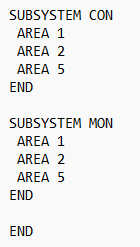
\includegraphics[scale=0.65]{sub.png}
   \caption{The subsystem file corresponding to Year 5 Topology 6} 
   \label{fig:sub}
\end{figure}

\begin{figure}[H]
   \centering 
   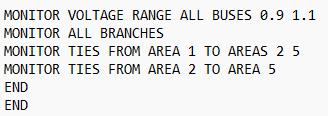
\includegraphics[scale=0.65]{mon.png}
   \caption{The monitored file corresponding to Year 5 Topology 6} 
   \label{fig:mon}
\end{figure}

\begin{figure}[H]
   \centering 
   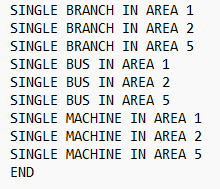
\includegraphics[scale=0.65]{con.png}
   \caption{The contingency file corresponding to Year 5 Topology 6} 
   \label{fig:con}
\end{figure}


For each of the 81 studied scenarios, the API DFAX\_2 is used to construct 81 different distribution factor data files corresponding to each .sav file, and the above defined .sub, .mon, .con configuration files.
For each of the 81 scenarios, by running the AC contingency calculation function ACCC\_WITH\_DSP\_3, the contingency solution output .acc files are obtained.

For each of the 81 scenarios, using the contingency solution output files, the results are exported as excel files for further analysis. The results exported are ACCC Analysis Summary, Monitored Branch Flows (MVA), Monitored Bus Voltages. 
 \newpage
Python code to conduct AC contingency calculation is:

\begin{python}
import psspy
list_gens = [0,50,100]
list_lsc = ['LLS','RLS','HLS']
list_gen_hydro = [400,500,600] #dry, average, wet hydological scenarios
list_gen_wind = [0,40,75] # for 3 wind gust scenarios
for gen in list_gens:
    for gen_hy in list_gen_hydro:
        for lsc in list_lsc:
            for gen_wi in list_gen_wind:
                file_in = 'sav\savnw_sol_' + str(gen) +'_hy_' +str(gen_hy) +'_wi_' + str(gen_wi) +'_' + str(lsc)+'.sav'
                file_dist = 'savnw_sol_' + str(gen) +'_hy_' +str(gen_hy) +'_wi_' + str(gen_wi) +'_' + str(lsc)+'.dfx'
                file_out = 'savnw_sol_' + str(gen) +'_hy_' +str(gen_hy) +'_wi_' + str(gen_wi) +'_' + str(lsc)+'.acc'
                file_sav = r"{}".format(file_in)
                file_dfx = r"{}".format(file_dist)
                file_acc = r"{}".format(file_out)
                psspy.case(file_in)
                psspy.fdns([0,1,0,0,0,0,0,0])
                psspy.dfax_2([1,1,0],r"""savnw.sub""",r"""savnw.mon""",r"""savnw.con""",file_dfx)
                psspy.accc_with_dsp_3(0.1,[0,1,0,0,0,0,0,0,0,0,0],"",file_dfx,file_acc,"","","")
\end{python}



Python code to export AC contingency solution output file as excel is: 

\begin{python}
import pssexcel
list_gens = [0,50,100]
list_lsc = ['LLS','RLS','HLS']
list_gen_hydro = [400,500,600] #dry, average, wet hydological scenarios
list_gen_wind = [0,40,75] # for 3 wind gust scenarios
for gen in list_gens:
    for gen_hy in list_gen_hydro:
        for lsc in list_lsc:
            for gen_wi in list_gen_wind:
                file_in = 'acc\savnw_sol_' + str(gen) +'_hy_' +str(gen_hy) +'_wi_' + str(gen_wi) +'_' + str(lsc)+'.acc'
                file_out = 'savnw_sol_' + str(gen) +'_hy_' +str(gen_hy) +'_wi_' + str(gen_wi) +'_' + str(lsc)+'.xlsx'
                file_acc = r"{}".format(file_in)
                file_xlsx = r"{}".format(file_out)
                pssexcel.accc(file_acc, ['s','v','b'], colabel='',stype='contingency', busmsm=0.5, sysmsm=5.0,
                        rating='a', namesplit=False,xlsfile=file_out, sheet='', overwritesheet=True, show=False, ratecon='b',
                        baseflowvio=True,basevoltvio=True, flowlimit=100.0, flowchange=0.0, voltchange=0.0,swdrating='a',
                        swdratecon='b',baseswdflowvio=False,basenodevoltvio=False,overloadreport=False)
\end{python}

Contingency analysis was carried out in PSSE for each of the studied scenario for Year 5, Topology 6. It was seen that the power flow solution did not converge for some of the tested contingencies for the studied scenario. 
For each of the scenario, the contingencies for which power flow solution did not converge are given in Tables \ref{nonconv}, \ref{nonconv1}, and \ref{nonconv2} Appendix \ref{chapter:app} of the document. 

For the converged contingencies for each of the studied scenario, the results of the contingency analysis were analysed to check for branch overload ($ > 100\%$) and out of range bus voltage violations (lower emergency limit $ < 0.9 PU $ and upper emergency limit $ > 1.1 PU$). It was seen that for some of the contingencies there were no branch overload or bus voltage violations reported. Rest of the contingencies violating branch overload and bus voltage emergency ranges are reported in the subsequent chapters. Chapter ~\ref{overload} of this document gives the observed branch flow violations for each of the studied scenario. Chapter ~\ref{upper} gives the upper voltage violations reported for each of the studied scenarios. Chapter ~\ref{lower} gives the lower voltage violations reported for each of the studied scenarios. To conclude, Chapter ~\ref{conclusion} summarises the result of the contingency analysis carried out on Year 5, Topology 6 of the hypothetical SAVNW system. 

\chapter{Branch Overload Violation}
\label{overload}
\section{Introduction}
In this chapter, for each of the studied scenario, the branches that are loaded more than 100\% of their rating is tabulated. Branches that are loaded more than 130\% of the rating are said to be severely/ critically loaded and are noted down for reporting as operating these branches for prolonged duration is not recommended for a safe and reliable power system.
\section{Solar = 0 MW, Hydro = 400 MW, Wind = 0 MW, LLS}
For the studied scenario Solar = 0 MW, Hydro = 400 MW, Wind = 0 MW, LLS, the branches that are loaded more than 100\% of their rating is given in Table ~\ref{OLSolar0MWHydro400MWWind0MWLLS}. A loading of greater than 130\% of the branch rating was reported for the branch 154-203(1) for bus fault contingency BUS 205 and for single line open contingency SING OPN LIN   6 152-153(1).
\begin{table}[H]
\caption{Contingencies causing branch flow greater than 100\% for scenario Solar = 0 MW, Hydro = 400 MW, Wind = 0 MW, LLS}
\label{OLSolar0MWHydro400MWWind0MWLLS}
\centering
\scalebox{0.75}{\begin{tabular}{llrrrr}
\toprule
Branch & Contingency & MVA Flow & AMP Flow & Rate & Loading \\
\midrule
3001-3003(1) & SING OPN LIN   1 101-151(1) & 386.80 & 379.16 & 300.00 & 126.39 \\
3001-3003(2) & SING OPN LIN   1 101-151(1) & 386.80 & 379.16 & 300.00 & 126.39 \\
3003-3005(1) & SING OPN LIN   1 101-151(1) & -375.04 & 379.38 & 350.00 & 108.39 \\
3003-3005(2) & SING OPN LIN   1 101-151(1) & -375.04 & 379.38 & 350.00 & 108.39 \\
101-151(1) & SING OPN LIN   2 102-151(1) & 1516.41 & 1516.41 & 1350.00 & 112.33 \\
154-203(1) & SING OPN LIN   6 152-153(1) & 298.16 & 328.73 & 250.00 & 131.49 \\
154-205(1) & SING OPN LIN   6 152-153(1) & 761.43 & 839.50 & 660.00 & 127.20 \\
154-203(1) & BUS 153 & 280.58 & 301.66 & 250.00 & 120.66 \\
154-205(1) & BUS 153 & 684.33 & 735.74 & 660.00 & 111.48 \\
153-154(1) & BUS 205 & -276.44 & 364.06 & 350.00 & 104.02 \\
154-203(1) & BUS 205 & 380.42 & 501.01 & 250.00 & 200.40 \\
3001-3003(1) & UNIT 101(1) & 386.87 & 379.23 & 300.00 & 126.41 \\
3001-3003(2) & UNIT 101(1) & 386.87 & 379.23 & 300.00 & 126.41 \\
3003-3005(1) & UNIT 101(1) & -375.11 & 379.45 & 350.00 & 108.41 \\
3003-3005(2) & UNIT 101(1) & -375.11 & 379.45 & 350.00 & 108.41 \\
101-151(1) & UNIT 102(1) & 1516.41 & 1516.41 & 1350.00 & 112.33 \\
\bottomrule
\end{tabular}}
\end{table}

\section{Solar = 0 MW, Hydro = 400 MW, Wind = 40 MW, LLS}
For the studied scenario Solar = 0 MW, Hydro = 400 MW, Wind = 40 MW, LLS, the branches that are loaded more than 100\% of their rating is given in Table ~\ref{OLSolar0MWHydro400MWWind40MWLLS}. A loading of greater than 130\% of the branch rating was reported for the branch 154-203(1) for bus fault contingency BUS 205 and for single line open contingency SING OPN LIN   6 152-153(1).
\begin{table}[H]
\caption{Contingencies causing branch flow greater than 100\% for scenario Solar = 0 MW, Hydro = 400 MW, Wind = 40 MW, LLS}
\label{OLSolar0MWHydro400MWWind40MWLLS}
\centering
\scalebox{0.75}{\begin{tabular}{llrrrr}
\toprule
Branch & Contingency & MVA Flow & AMP Flow & Rate & Loading \\
\midrule
3001-3003(1) & SING OPN LIN   1 101-151(1) & 372.04 & 364.19 & 300.00 & 121.40 \\
3001-3003(2) & SING OPN LIN   1 101-151(1) & 372.04 & 364.19 & 300.00 & 121.40 \\
3003-3005(1) & SING OPN LIN   1 101-151(1) & -361.05 & 364.44 & 350.00 & 104.13 \\
3003-3005(2) & SING OPN LIN   1 101-151(1) & -361.05 & 364.44 & 350.00 & 104.13 \\
101-151(1) & SING OPN LIN   2 102-151(1) & 1516.48 & 1516.48 & 1350.00 & 112.33 \\
154-203(1) & SING OPN LIN   6 152-153(1) & 296.13 & 325.81 & 250.00 & 130.32 \\
154-205(1) & SING OPN LIN   6 152-153(1) & 755.65 & 831.37 & 660.00 & 125.97 \\
154-203(1) & BUS 153 & 280.16 & 301.04 & 250.00 & 120.41 \\
154-205(1) & BUS 153 & 683.04 & 733.93 & 660.00 & 111.20 \\
153-154(1) & BUS 203 & -324.87 & 350.28 & 350.00 & 100.08 \\
153-154(1) & BUS 205 & -278.20 & 369.32 & 350.00 & 105.52 \\
154-203(1) & BUS 205 & 381.33 & 506.23 & 250.00 & 202.49 \\
3001-3003(1) & UNIT 101(1) & 372.11 & 364.26 & 300.00 & 121.42 \\
3001-3003(2) & UNIT 101(1) & 372.11 & 364.26 & 300.00 & 121.42 \\
3003-3005(1) & UNIT 101(1) & -361.11 & 364.50 & 350.00 & 104.14 \\
3003-3005(2) & UNIT 101(1) & -361.11 & 364.50 & 350.00 & 104.14 \\
101-151(1) & UNIT 102(1) & 1516.48 & 1516.48 & 1350.00 & 112.33 \\
\bottomrule
\end{tabular}}
\end{table}

\section{Solar = 0 MW, Hydro = 400 MW, Wind = 75 MW, LLS}
For the studied scenario Solar = 0 MW, Hydro = 400 MW, Wind = 75 MW, LLS, the branches that are loaded more than 100\% of their rating is given in Table ~\ref{OLSolar0MWHydro400MWWind75MWLLS}. No branches reported a loading greater than 130\% of the branch rating.
\begin{table}[H]
\caption{Contingencies causing branch flow greater than 100\% for scenario Solar = 0 MW, Hydro = 400 MW, Wind = 75 MW, LLS}
\label{OLSolar0MWHydro400MWWind75MWLLS}
\centering
\scalebox{0.75}{\begin{tabular}{llrrrr}
\toprule
Branch & Contingency & MVA Flow & AMP Flow & Rate & Loading \\
\midrule
3001-3003(1) & SING OPN LIN   1 101-151(1) & 359.49 & 351.54 & 300.00 & 117.18 \\
3001-3003(2) & SING OPN LIN   1 101-151(1) & 359.49 & 351.54 & 300.00 & 117.18 \\
3003-3005(1) & SING OPN LIN   1 101-151(1) & -349.05 & 351.82 & 350.00 & 100.52 \\
3003-3005(2) & SING OPN LIN   1 101-151(1) & -349.05 & 351.82 & 350.00 & 100.52 \\
101-151(1) & SING OPN LIN   2 102-151(1) & 1516.60 & 1516.60 & 1350.00 & 112.34 \\
154-203(1) & SING OPN LIN   6 152-153(1) & 294.57 & 324.01 & 250.00 & 129.60 \\
154-205(1) & SING OPN LIN   6 152-153(1) & 751.86 & 827.00 & 660.00 & 125.30 \\
154-203(1) & BUS 153 & 279.92 & 300.86 & 250.00 & 120.34 \\
154-205(1) & BUS 153 & 682.60 & 733.65 & 660.00 & 111.16 \\
153-154(1) & BUS 203 & -326.44 & 352.21 & 350.00 & 100.63 \\
3001-3003(1) & UNIT 101(1) & 359.55 & 351.61 & 300.00 & 117.20 \\
3001-3003(2) & UNIT 101(1) & 359.55 & 351.61 & 300.00 & 117.20 \\
3003-3005(1) & UNIT 101(1) & -349.11 & 351.89 & 350.00 & 100.54 \\
3003-3005(2) & UNIT 101(1) & -349.11 & 351.89 & 350.00 & 100.54 \\
101-151(1) & UNIT 102(1) & 1516.60 & 1516.60 & 1350.00 & 112.34 \\
\bottomrule
\end{tabular}}
\end{table}

\section{Solar = 0 MW, Hydro = 400 MW, Wind = 0 MW, RLS}
For the studied scenario Solar = 0 MW, Hydro = 400 MW, Wind = 0 MW, RLS, the branches that are loaded more than 100\% of their rating is given in Table ~\ref{OLSolar0MWHydro400MWWind0MWRLS}. A loading of greater than 130\% of the branch rating were reported for the branches: 3001-3003(1), 3001-3003(2) for unit fault contingency UNIT 101(1); 154-203(1) for bus fault contingency BUS 153; 154-203(1), 154-205(1) for single line open contingency SING OPN LIN   6 152-153(1); 3001-3003(1), 3001-3003(2) for single line open contingency SING OPN LIN   1 101-151(1).
\begin{table}[H]
\caption{Contingencies causing branch flow greater than 100\% for scenario Solar = 0 MW, Hydro = 400 MW, Wind = 0 MW, RLS}
\label{OLSolar0MWHydro400MWWind0MWRLS}
\centering
\scalebox{0.75}{\begin{tabular}{llrrrr}
\toprule
Branch & Contingency & MVA Flow & AMP Flow & Rate & Loading \\
\midrule
3001-3003(1) & SING OPN LIN   1 101-151(1) & 428.13 & 424.23 & 300.00 & 141.41 \\
3001-3003(2) & SING OPN LIN   1 101-151(1) & 428.13 & 424.23 & 300.00 & 141.41 \\
3003-3005(1) & SING OPN LIN   1 101-151(1) & -408.26 & 424.87 & 350.00 & 121.39 \\
3003-3005(2) & SING OPN LIN   1 101-151(1) & -408.26 & 424.87 & 350.00 & 121.39 \\
101-151(1) & SING OPN LIN   2 102-151(1) & 1594.72 & 1594.72 & 1350.00 & 118.13 \\
154-203(1) & SING OPN LIN   6 152-153(1) & 310.70 & 364.11 & 250.00 & 145.64 \\
154-205(1) & SING OPN LIN   6 152-153(1) & 812.73 & 952.43 & 660.00 & 144.31 \\
203-205(1) & SING OPN LIN   6 152-153(1) & -220.00 & 253.11 & 250.00 & 101.24 \\
203-205(2) & SING OPN LIN   6 152-153(1) & -220.00 & 253.11 & 250.00 & 101.24 \\
205-206(1) & SING OPN LIN   12 201-211(1) & -1291.26 & 1291.26 & 1250.00 & 103.30 \\
205-206(1) & SING OPN LIN   13 201-212(1) & -1291.26 & 1291.26 & 1250.00 & 103.30 \\
154-203(1) & BUS 153 & 293.58 & 331.95 & 250.00 & 132.78 \\
154-205(1) & BUS 153 & 731.49 & 827.08 & 660.00 & 125.31 \\
153-154(1) & BUS 203 & -336.33 & 380.69 & 350.00 & 108.77 \\
154-203(1) & BUS 3005 & 229.20 & 273.34 & 250.00 & 109.33 \\
154-205(1) & BUS 3005 & 641.30 & 764.78 & 660.00 & 115.88 \\
154-3008(1) & BUS 3005 & -363.01 & 458.49 & 440.00 & 104.20 \\
3001-3003(1) & UNIT 101(1) & 428.30 & 424.41 & 300.00 & 141.47 \\
3001-3003(2) & UNIT 101(1) & 428.30 & 424.41 & 300.00 & 141.47 \\
3003-3005(1) & UNIT 101(1) & -408.40 & 425.04 & 350.00 & 121.44 \\
3003-3005(2) & UNIT 101(1) & -408.40 & 425.04 & 350.00 & 121.44 \\
101-151(1) & UNIT 102(1) & 1594.72 & 1594.72 & 1350.00 & 118.13 \\
205-206(1) & UNIT 211(1) & -1289.97 & 1289.97 & 1250.00 & 103.20 \\
205-206(1) & UNIT 212(1) & -1289.97 & 1289.97 & 1250.00 & 103.20 \\
\bottomrule
\end{tabular}}
\end{table}

\section{Solar = 0 MW, Hydro = 400 MW, Wind = 40 MW, RLS}
For the studied scenario Solar = 0 MW, Hydro = 400 MW, Wind = 40 MW, RLS, the branches that are loaded more than 100\% of their rating is given in Table ~\ref{OLSolar0MWHydro400MWWind40MWRLS}. A loading of greater than 130\% of the branch rating were reported for the branches: 3001-3003(1), 3001-3003(2) for unit fault contingency UNIT 101(1); 154-203(1) for bus fault contingency BUS 153; 154-203(1), 154-205(1) for single line open contingency SING OPN LIN   6 152-153(1); 3001-3003(1), 3001-3003(2) for single line open contingency SING OPN LIN   1 101-151(1).
\begin{table}[H]
\caption{Contingencies causing branch flow greater than 100\% for scenario Solar = 0 MW, Hydro = 400 MW, Wind = 40 MW, RLS}
\label{OLSolar0MWHydro400MWWind40MWRLS}
\centering
\scalebox{0.75}{\begin{tabular}{llrrrr}
\toprule
Branch & Contingency & MVA Flow & AMP Flow & Rate & Loading \\
\midrule
3001-3003(1) & SING OPN LIN   1 101-151(1) & 412.73 & 408.08 & 300.00 & 136.03 \\
3001-3003(2) & SING OPN LIN   1 101-151(1) & 412.73 & 408.08 & 300.00 & 136.03 \\
3003-3005(1) & SING OPN LIN   1 101-151(1) & -394.42 & 408.72 & 350.00 & 116.78 \\
3003-3005(2) & SING OPN LIN   1 101-151(1) & -394.42 & 408.72 & 350.00 & 116.78 \\
101-151(1) & SING OPN LIN   2 102-151(1) & 1594.66 & 1594.66 & 1350.00 & 118.12 \\
154-203(1) & SING OPN LIN   6 152-153(1) & 308.70 & 360.63 & 250.00 & 144.25 \\
154-205(1) & SING OPN LIN   6 152-153(1) & 806.76 & 942.47 & 660.00 & 142.80 \\
203-205(1) & SING OPN LIN   6 152-153(1) & -218.60 & 250.76 & 250.00 & 100.31 \\
203-205(2) & SING OPN LIN   6 152-153(1) & -218.60 & 250.76 & 250.00 & 100.31 \\
205-206(1) & SING OPN LIN   12 201-211(1) & -1291.09 & 1291.09 & 1250.00 & 103.29 \\
205-206(1) & SING OPN LIN   13 201-212(1) & -1291.09 & 1291.09 & 1250.00 & 103.29 \\
154-203(1) & BUS 153 & 293.17 & 331.22 & 250.00 & 132.49 \\
154-205(1) & BUS 153 & 730.17 & 824.93 & 660.00 & 124.99 \\
153-154(1) & BUS 203 & -338.16 & 382.66 & 350.00 & 109.33 \\
154-203(1) & BUS 3005 & 228.23 & 271.14 & 250.00 & 108.46 \\
154-205(1) & BUS 3005 & 637.39 & 757.22 & 660.00 & 114.73 \\
154-3008(1) & BUS 3005 & -362.85 & 456.22 & 440.00 & 103.69 \\
3001-3003(1) & UNIT 101(1) & 412.89 & 408.24 & 300.00 & 136.08 \\
3001-3003(2) & UNIT 101(1) & 412.89 & 408.24 & 300.00 & 136.08 \\
3003-3005(1) & UNIT 101(1) & -394.56 & 408.88 & 350.00 & 116.82 \\
3003-3005(2) & UNIT 101(1) & -394.56 & 408.88 & 350.00 & 116.82 \\
101-151(1) & UNIT 102(1) & 1594.66 & 1594.66 & 1350.00 & 118.12 \\
205-206(1) & UNIT 211(1) & -1289.83 & 1289.83 & 1250.00 & 103.19 \\
205-206(1) & UNIT 212(1) & -1289.83 & 1289.83 & 1250.00 & 103.19 \\
\bottomrule
\end{tabular}}
\end{table}

\section{Solar = 0 MW, Hydro = 400 MW, Wind = 75 MW, RLS}
For the studied scenario Solar = 0 MW, Hydro = 400 MW, Wind = 75 MW, RLS, the branches that are loaded more than 100\% of their rating is given in Table ~\ref{OLSolar0MWHydro400MWWind75MWRLS}. A loading of greater than 130\% of the branch rating were reported for the branches: 3001-3003(1), 3001-3003(2) for unit fault contingency UNIT 101(1); 154-203(1) for bus fault contingency BUS 153; 154-203(1), 154-205(1) for single line open contingency SING OPN LIN   6 152-153(1); 3001-3003(1), 3001-3003(2) for single line open contingency SING OPN LIN   1 101-151(1).
\begin{table}[H]
\caption{Contingencies causing branch flow greater than 100\% for scenario Solar = 0 MW, Hydro = 400 MW, Wind = 75 MW, RLS}
\label{OLSolar0MWHydro400MWWind75MWRLS}
\centering
\scalebox{0.75}{\begin{tabular}{llrrrr}
\toprule
Branch & Contingency & MVA Flow & AMP Flow & Rate & Loading \\
\midrule
3001-3003(1) & SING OPN LIN   1 101-151(1) & 399.83 & 394.71 & 300.00 & 131.57 \\
3001-3003(2) & SING OPN LIN   1 101-151(1) & 399.83 & 394.71 & 300.00 & 131.57 \\
3003-3005(1) & SING OPN LIN   1 101-151(1) & -382.59 & 395.37 & 350.00 & 112.96 \\
3003-3005(2) & SING OPN LIN   1 101-151(1) & -382.59 & 395.37 & 350.00 & 112.96 \\
101-151(1) & SING OPN LIN   2 102-151(1) & 1594.83 & 1594.83 & 1350.00 & 118.14 \\
154-203(1) & SING OPN LIN   6 152-153(1) & 307.24 & 358.80 & 250.00 & 143.52 \\
154-205(1) & SING OPN LIN   6 152-153(1) & 802.93 & 937.68 & 660.00 & 142.07 \\
205-206(1) & SING OPN LIN   12 201-211(1) & -1291.03 & 1291.03 & 1250.00 & 103.28 \\
205-206(1) & SING OPN LIN   13 201-212(1) & -1291.03 & 1291.03 & 1250.00 & 103.28 \\
154-203(1) & BUS 153 & 292.96 & 331.09 & 250.00 & 132.44 \\
154-205(1) & BUS 153 & 729.74 & 824.72 & 660.00 & 124.96 \\
153-154(1) & BUS 203 & -339.61 & 384.65 & 350.00 & 109.90 \\
154-203(1) & BUS 3005 & 227.64 & 270.28 & 250.00 & 108.11 \\
154-205(1) & BUS 3005 & 635.70 & 754.79 & 660.00 & 114.36 \\
154-3008(1) & BUS 3005 & -362.83 & 455.89 & 440.00 & 103.61 \\
3001-3003(1) & UNIT 101(1) & 399.98 & 394.87 & 300.00 & 131.62 \\
3001-3003(2) & UNIT 101(1) & 399.98 & 394.87 & 300.00 & 131.62 \\
3003-3005(1) & UNIT 101(1) & -382.73 & 395.53 & 350.00 & 113.01 \\
3003-3005(2) & UNIT 101(1) & -382.73 & 395.53 & 350.00 & 113.01 \\
101-151(1) & UNIT 102(1) & 1594.83 & 1594.83 & 1350.00 & 118.14 \\
205-206(1) & UNIT 211(1) & -1289.72 & 1289.72 & 1250.00 & 103.18 \\
205-206(1) & UNIT 212(1) & -1289.72 & 1289.72 & 1250.00 & 103.18 \\
\bottomrule
\end{tabular}}
\end{table}

\section{Solar = 0 MW, Hydro = 400 MW, Wind = 0 MW, HLS}
For the studied scenario Solar = 0 MW, Hydro = 400 MW, Wind = 0 MW, HLS, the branches that are loaded more than 100\% of their rating is given in Table ~\ref{OLSolar0MWHydro400MWWind0MWHLS}. A loading of greater than 130\% of the branch rating were reported for the branches: 3001-3003(1), 3001-3003(2), 3003-3005(1), 3003-3005(2) for single line open contingency SING OPN LIN   1 101-151(1); 3001-3003(1), 3001-3003(2), 3003-3005(1), 3003-3005(2) for unit fault contingency UNIT 101(1); 154-203(1), 154-205(1) for bus fault contingency BUS 153.
\begin{table}[H]
\caption{Contingencies causing branch flow greater than 100\% for scenario Solar = 0 MW, Hydro = 400 MW, Wind = 0 MW, HLS}
\label{OLSolar0MWHydro400MWWind0MWHLS}
\centering
\scalebox{0.75}{\begin{tabular}{llrrrr}
\toprule
Branch & Contingency & MVA Flow & AMP Flow & Rate & Loading \\
\midrule
3001-3003(1) & SING OPN LIN   1 101-151(1) & 463.69 & 464.38 & 300.00 & 154.79 \\
3001-3003(2) & SING OPN LIN   1 101-151(1) & 463.69 & 464.38 & 300.00 & 154.79 \\
3003-3005(1) & SING OPN LIN   1 101-151(1) & -434.60 & 465.34 & 350.00 & 132.95 \\
3003-3005(2) & SING OPN LIN   1 101-151(1) & -434.60 & 465.34 & 350.00 & 132.95 \\
101-151(1) & SING OPN LIN   2 102-151(1) & 1660.01 & 1660.01 & 1350.00 & 122.96 \\
205-206(1) & SING OPN LIN   12 201-211(1) & -1354.66 & 1354.66 & 1250.00 & 108.37 \\
205-206(1) & SING OPN LIN   13 201-212(1) & -1354.66 & 1354.66 & 1250.00 & 108.37 \\
154-203(1) & BUS 153 & 305.41 & 365.08 & 250.00 & 146.03 \\
154-205(1) & BUS 153 & 768.20 & 918.27 & 660.00 & 139.13 \\
203-205(1) & BUS 153 & -218.75 & 256.38 & 250.00 & 102.55 \\
203-205(2) & BUS 153 & -218.75 & 256.38 & 250.00 & 102.55 \\
153-154(1) & BUS 203 & -347.32 & 413.98 & 350.00 & 118.28 \\
3001-3003(1) & UNIT 101(1) & 463.72 & 464.41 & 300.00 & 154.80 \\
3001-3003(2) & UNIT 101(1) & 463.72 & 464.41 & 300.00 & 154.80 \\
3003-3005(1) & UNIT 101(1) & -434.63 & 465.37 & 350.00 & 132.96 \\
3003-3005(2) & UNIT 101(1) & -434.63 & 465.37 & 350.00 & 132.96 \\
101-151(1) & UNIT 102(1) & 1660.00 & 1660.00 & 1350.00 & 122.96 \\
205-206(1) & UNIT 211(1) & -1354.27 & 1354.27 & 1250.00 & 108.34 \\
205-206(1) & UNIT 212(1) & -1354.27 & 1354.27 & 1250.00 & 108.34 \\
\bottomrule
\end{tabular}}
\end{table}

\section{Solar = 0 MW, Hydro = 400 MW, Wind = 40 MW, HLS}
For the studied scenario Solar = 0 MW, Hydro = 400 MW, Wind = 40 MW, HLS, the branches that are loaded more than 100\% of their rating is given in Table ~\ref{OLSolar0MWHydro400MWWind40MWHLS}. A loading of greater than 130\% of the branch rating were reported for the branches: 3001-3003(1), 3001-3003(2) for unit fault contingency UNIT 101(1); 154-203(1), 154-205(1) for bus fault contingency BUS 153; 3001-3003(1), 3001-3003(2) for single line open contingency SING OPN LIN   1 101-151(1).
\begin{table}[H]
\caption{Contingencies causing branch flow greater than 100\% for scenario Solar = 0 MW, Hydro = 400 MW, Wind = 40 MW, HLS}
\label{OLSolar0MWHydro400MWWind40MWHLS}
\centering
\scalebox{0.75}{\begin{tabular}{llrrrr}
\toprule
Branch & Contingency & MVA Flow & AMP Flow & Rate & Loading \\
\midrule
3001-3003(1) & SING OPN LIN   1 101-151(1) & 447.71 & 447.18 & 300.00 & 149.06 \\
3001-3003(2) & SING OPN LIN   1 101-151(1) & 447.71 & 447.18 & 300.00 & 149.06 \\
3003-3005(1) & SING OPN LIN   1 101-151(1) & -420.85 & 448.15 & 350.00 & 128.04 \\
3003-3005(2) & SING OPN LIN   1 101-151(1) & -420.85 & 448.15 & 350.00 & 128.04 \\
101-151(1) & SING OPN LIN   2 102-151(1) & 1659.87 & 1659.87 & 1350.00 & 122.95 \\
205-206(1) & SING OPN LIN   12 201-211(1) & -1354.44 & 1354.44 & 1250.00 & 108.35 \\
205-206(1) & SING OPN LIN   13 201-212(1) & -1354.44 & 1354.44 & 1250.00 & 108.35 \\
154-203(1) & BUS 153 & 305.01 & 364.18 & 250.00 & 145.67 \\
154-205(1) & BUS 153 & 766.86 & 915.63 & 660.00 & 138.73 \\
203-205(1) & BUS 153 & -218.46 & 255.77 & 250.00 & 102.31 \\
203-205(2) & BUS 153 & -218.46 & 255.77 & 250.00 & 102.31 \\
153-154(1) & BUS 203 & -349.39 & 416.46 & 350.00 & 118.99 \\
3001-3003(1) & UNIT 101(1) & 447.74 & 447.21 & 300.00 & 149.07 \\
3001-3003(2) & UNIT 101(1) & 447.74 & 447.21 & 300.00 & 149.07 \\
3003-3005(1) & UNIT 101(1) & -420.87 & 448.18 & 350.00 & 128.05 \\
3003-3005(2) & UNIT 101(1) & -420.87 & 448.18 & 350.00 & 128.05 \\
101-151(1) & UNIT 102(1) & 1659.86 & 1659.86 & 1350.00 & 122.95 \\
205-206(1) & UNIT 211(1) & -1354.06 & 1354.06 & 1250.00 & 108.32 \\
205-206(1) & UNIT 212(1) & -1354.06 & 1354.06 & 1250.00 & 108.32 \\
\bottomrule
\end{tabular}}
\end{table}

\section{Solar = 0 MW, Hydro = 400 MW, Wind = 75 MW, HLS}
For the studied scenario Solar = 0 MW, Hydro = 400 MW, Wind = 75 MW, HLS, the branches that are loaded more than 100\% of their rating is given in Table ~\ref{OLSolar0MWHydro400MWWind75MWHLS}. A loading of greater than 130\% of the branch rating were reported for the branches: 3001-3003(1), 3001-3003(2) for unit fault contingency UNIT 101(1); 154-203(1), 154-205(1) for bus fault contingency BUS 153; 3001-3003(1), 3001-3003(2) for single line open contingency SING OPN LIN   1 101-151(1).
\begin{table}[H]
\caption{Contingencies causing branch flow greater than 100\% for scenario Solar = 0 MW, Hydro = 400 MW, Wind = 75 MW, HLS}
\label{OLSolar0MWHydro400MWWind75MWHLS}
\centering
\scalebox{0.75}{\begin{tabular}{llrrrr}
\toprule
Branch & Contingency & MVA Flow & AMP Flow & Rate & Loading \\
\midrule
3001-3003(1) & SING OPN LIN   1 101-151(1) & 434.45 & 433.10 & 300.00 & 144.37 \\
3001-3003(2) & SING OPN LIN   1 101-151(1) & 434.45 & 433.10 & 300.00 & 144.37 \\
3003-3005(1) & SING OPN LIN   1 101-151(1) & -409.09 & 434.10 & 350.00 & 124.03 \\
3003-3005(2) & SING OPN LIN   1 101-151(1) & -409.09 & 434.10 & 350.00 & 124.03 \\
101-151(1) & SING OPN LIN   2 102-151(1) & 1660.05 & 1660.05 & 1350.00 & 122.97 \\
205-206(1) & SING OPN LIN   12 201-211(1) & -1354.32 & 1354.32 & 1250.00 & 108.35 \\
205-206(1) & SING OPN LIN   13 201-212(1) & -1354.32 & 1354.32 & 1250.00 & 108.35 \\
154-203(1) & BUS 153 & 304.84 & 364.14 & 250.00 & 145.66 \\
154-205(1) & BUS 153 & 766.44 & 915.54 & 660.00 & 138.72 \\
203-205(1) & BUS 153 & -218.35 & 255.75 & 250.00 & 102.30 \\
203-205(2) & BUS 153 & -218.35 & 255.75 & 250.00 & 102.30 \\
153-154(1) & BUS 203 & -350.54 & 418.56 & 350.00 & 119.59 \\
3001-3003(1) & UNIT 101(1) & 434.47 & 433.13 & 300.00 & 144.38 \\
3001-3003(2) & UNIT 101(1) & 434.47 & 433.13 & 300.00 & 144.38 \\
3003-3005(1) & UNIT 101(1) & -409.12 & 434.13 & 350.00 & 124.04 \\
3003-3005(2) & UNIT 101(1) & -409.12 & 434.13 & 350.00 & 124.04 \\
101-151(1) & UNIT 102(1) & 1660.04 & 1660.04 & 1350.00 & 122.97 \\
205-206(1) & UNIT 211(1) & -1353.94 & 1353.94 & 1250.00 & 108.31 \\
205-206(1) & UNIT 212(1) & -1353.94 & 1353.94 & 1250.00 & 108.31 \\
\bottomrule
\end{tabular}}
\end{table}

\section{Solar = 0 MW, Hydro = 500 MW, Wind = 0 MW, LLS}
For the studied scenario Solar = 0 MW, Hydro = 500 MW, Wind = 0 MW, LLS, the branches that are loaded more than 100\% of their rating is given in Table ~\ref{OLSolar0MWHydro500MWWind0MWLLS}. A loading of greater than 130\% of the branch rating was reported for the branch 154-203(1) for bus fault contingency BUS 153 and for single line open contingency SING OPN LIN   6 152-153(1).
\begin{table}[H]
\caption{Contingencies causing branch flow greater than 100\% for scenario Solar = 0 MW, Hydro = 500 MW, Wind = 0 MW, LLS}
\label{OLSolar0MWHydro500MWWind0MWLLS}
\centering
\scalebox{0.75}{\begin{tabular}{llrrrr}
\toprule
Branch & Contingency & MVA Flow & AMP Flow & Rate & Loading \\
\midrule
3001-3003(1) & SING OPN LIN   1 101-151(1) & 389.00 & 381.91 & 300.00 & 127.30 \\
3001-3003(2) & SING OPN LIN   1 101-151(1) & 389.00 & 381.91 & 300.00 & 127.30 \\
3003-3005(1) & SING OPN LIN   1 101-151(1) & -376.07 & 382.24 & 350.00 & 109.21 \\
3003-3005(2) & SING OPN LIN   1 101-151(1) & -376.07 & 382.24 & 350.00 & 109.21 \\
101-151(1) & SING OPN LIN   2 102-151(1) & 1520.99 & 1520.99 & 1350.00 & 112.67 \\
154-203(1) & SING OPN LIN   6 152-153(1) & 319.52 & 358.62 & 250.00 & 143.45 \\
154-205(1) & SING OPN LIN   6 152-153(1) & 717.75 & 805.57 & 660.00 & 122.06 \\
203-205(1) & SING OPN LIN   6 152-153(1) & -235.67 & 260.33 & 250.00 & 104.13 \\
203-205(2) & SING OPN LIN   6 152-153(1) & -235.67 & 260.33 & 250.00 & 104.13 \\
154-203(1) & BUS 153 & 303.93 & 331.99 & 250.00 & 132.80 \\
154-205(1) & BUS 153 & 644.21 & 703.68 & 660.00 & 106.62 \\
153-154(1) & BUS 203 & -349.70 & 387.51 & 350.00 & 110.72 \\
154-203(1) & BUS 3005 & 229.34 & 257.53 & 250.00 & 103.01 \\
3001-3003(1) & UNIT 101(1) & 389.08 & 381.99 & 300.00 & 127.33 \\
3001-3003(2) & UNIT 101(1) & 389.08 & 381.99 & 300.00 & 127.33 \\
3003-3005(1) & UNIT 101(1) & -376.14 & 382.32 & 350.00 & 109.23 \\
3003-3005(2) & UNIT 101(1) & -376.14 & 382.32 & 350.00 & 109.23 \\
101-151(1) & UNIT 102(1) & 1520.99 & 1520.99 & 1350.00 & 112.67 \\
\bottomrule
\end{tabular}}
\end{table}

\section{Solar = 0 MW, Hydro = 500 MW, Wind = 40 MW, LLS}
For the studied scenario Solar = 0 MW, Hydro = 500 MW, Wind = 40 MW, LLS, the branches that are loaded more than 100\% of their rating is given in Table ~\ref{OLSolar0MWHydro500MWWind40MWLLS}. A loading of greater than 130\% of the branch rating was reported for the branch 154-203(1) for bus fault contingency BUS 153 and for single line open contingency SING OPN LIN   6 152-153(1).
\begin{table}[H]
\caption{Contingencies causing branch flow greater than 100\% for scenario Solar = 0 MW, Hydro = 500 MW, Wind = 40 MW, LLS}
\label{OLSolar0MWHydro500MWWind40MWLLS}
\centering
\scalebox{0.75}{\begin{tabular}{llrrrr}
\toprule
Branch & Contingency & MVA Flow & AMP Flow & Rate & Loading \\
\midrule
3001-3003(1) & SING OPN LIN   1 101-151(1) & 374.04 & 366.57 & 300.00 & 122.19 \\
3001-3003(2) & SING OPN LIN   1 101-151(1) & 374.04 & 366.57 & 300.00 & 122.19 \\
3003-3005(1) & SING OPN LIN   1 101-151(1) & -362.20 & 366.90 & 350.00 & 104.83 \\
3003-3005(2) & SING OPN LIN   1 101-151(1) & -362.20 & 366.90 & 350.00 & 104.83 \\
101-151(1) & SING OPN LIN   2 102-151(1) & 1521.01 & 1521.01 & 1350.00 & 112.67 \\
154-203(1) & SING OPN LIN   6 152-153(1) & 317.54 & 355.54 & 250.00 & 142.22 \\
154-205(1) & SING OPN LIN   6 152-153(1) & 711.88 & 797.09 & 660.00 & 120.77 \\
203-205(1) & SING OPN LIN   6 152-153(1) & -234.30 & 258.23 & 250.00 & 103.29 \\
203-205(2) & SING OPN LIN   6 152-153(1) & -234.30 & 258.23 & 250.00 & 103.29 \\
154-203(1) & BUS 153 & 303.52 & 331.33 & 250.00 & 132.53 \\
154-205(1) & BUS 153 & 642.92 & 701.83 & 660.00 & 106.34 \\
153-154(1) & BUS 203 & -351.62 & 389.56 & 350.00 & 111.30 \\
154-203(1) & BUS 3005 & 228.39 & 255.87 & 250.00 & 102.35 \\
3001-3003(1) & UNIT 101(1) & 374.12 & 366.65 & 300.00 & 122.22 \\
3001-3003(2) & UNIT 101(1) & 374.12 & 366.65 & 300.00 & 122.22 \\
3003-3005(1) & UNIT 101(1) & -362.27 & 366.98 & 350.00 & 104.85 \\
3003-3005(2) & UNIT 101(1) & -362.27 & 366.98 & 350.00 & 104.85 \\
101-151(1) & UNIT 102(1) & 1521.01 & 1521.01 & 1350.00 & 112.67 \\
\bottomrule
\end{tabular}}
\end{table}

\section{Solar = 0 MW, Hydro = 500 MW, Wind = 75 MW, LLS}
For the studied scenario Solar = 0 MW, Hydro = 500 MW, Wind = 75 MW, LLS, the branches that are loaded more than 100\% of their rating is given in Table ~\ref{OLSolar0MWHydro500MWWind75MWLLS}. A loading of greater than 130\% of the branch rating was reported for the branch 154-203(1) for bus fault contingency BUS 153 and for single line open contingency SING OPN LIN   6 152-153(1).
\begin{table}[H]
\caption{Contingencies causing branch flow greater than 100\% for scenario Solar = 0 MW, Hydro = 500 MW, Wind = 75 MW, LLS}
\label{OLSolar0MWHydro500MWWind75MWLLS}
\centering
\scalebox{0.75}{\begin{tabular}{llrrrr}
\toprule
Branch & Contingency & MVA Flow & AMP Flow & Rate & Loading \\
\midrule
3001-3003(1) & SING OPN LIN   1 101-151(1) & 361.40 & 353.75 & 300.00 & 117.92 \\
3001-3003(2) & SING OPN LIN   1 101-151(1) & 361.40 & 353.75 & 300.00 & 117.92 \\
3003-3005(1) & SING OPN LIN   1 101-151(1) & -350.30 & 354.10 & 350.00 & 101.17 \\
3003-3005(2) & SING OPN LIN   1 101-151(1) & -350.30 & 354.10 & 350.00 & 101.17 \\
101-151(1) & SING OPN LIN   2 102-151(1) & 1520.90 & 1520.90 & 1350.00 & 112.66 \\
154-203(1) & SING OPN LIN   6 152-153(1) & 315.98 & 353.69 & 250.00 & 141.47 \\
154-205(1) & SING OPN LIN   6 152-153(1) & 708.17 & 792.69 & 660.00 & 120.10 \\
203-205(1) & SING OPN LIN   6 152-153(1) & -233.19 & 256.93 & 250.00 & 102.77 \\
203-205(2) & SING OPN LIN   6 152-153(1) & -233.19 & 256.93 & 250.00 & 102.77 \\
154-203(1) & BUS 153 & 303.27 & 331.16 & 250.00 & 132.46 \\
154-205(1) & BUS 153 & 642.55 & 701.64 & 660.00 & 106.31 \\
153-154(1) & BUS 203 & -353.15 & 391.60 & 350.00 & 111.88 \\
154-203(1) & BUS 3005 & 227.70 & 255.04 & 250.00 & 102.01 \\
3001-3003(1) & UNIT 101(1) & 361.35 & 353.70 & 300.00 & 117.90 \\
3001-3003(2) & UNIT 101(1) & 361.35 & 353.70 & 300.00 & 117.90 \\
3003-3005(1) & UNIT 101(1) & -350.26 & 354.05 & 350.00 & 101.16 \\
3003-3005(2) & UNIT 101(1) & -350.26 & 354.05 & 350.00 & 101.16 \\
101-151(1) & UNIT 102(1) & 1520.90 & 1520.90 & 1350.00 & 112.66 \\
\bottomrule
\end{tabular}}
\end{table}

\section{Solar = 0 MW, Hydro = 500 MW, Wind = 0 MW, RLS}
For the studied scenario Solar = 0 MW, Hydro = 500 MW, Wind = 0 MW, RLS, the branches that are loaded more than 100\% of their rating is given in Table ~\ref{OLSolar0MWHydro500MWWind0MWRLS}. A loading of greater than 130\% of the branch rating were reported for the branches: 3001-3003(1), 3001-3003(2) for unit fault contingency UNIT 101(1); 154-203(1) for bus fault contingency BUS 153; 154-203(1), 154-205(1) for single line open contingency SING OPN LIN   6 152-153(1); 3001-3003(1), 3001-3003(2) for single line open contingency SING OPN LIN   1 101-151(1).
\begin{table}[H]
\caption{Contingencies causing branch flow greater than 100\% for scenario Solar = 0 MW, Hydro = 500 MW, Wind = 0 MW, RLS}
\label{OLSolar0MWHydro500MWWind0MWRLS}
\centering
\scalebox{0.75}{\begin{tabular}{llrrrr}
\toprule
Branch & Contingency & MVA Flow & AMP Flow & Rate & Loading \\
\midrule
3001-3003(1) & SING OPN LIN   1 101-151(1) & 431.55 & 428.41 & 300.00 & 142.80 \\
3001-3003(2) & SING OPN LIN   1 101-151(1) & 431.55 & 428.41 & 300.00 & 142.80 \\
3003-3005(1) & SING OPN LIN   1 101-151(1) & -410.03 & 429.14 & 350.00 & 122.61 \\
3003-3005(2) & SING OPN LIN   1 101-151(1) & -410.03 & 429.14 & 350.00 & 122.61 \\
101-151(1) & SING OPN LIN   2 102-151(1) & 1600.53 & 1600.53 & 1350.00 & 118.56 \\
154-203(1) & SING OPN LIN   6 152-153(1) & 331.55 & 398.40 & 250.00 & 159.36 \\
154-205(1) & SING OPN LIN   6 152-153(1) & 766.93 & 921.57 & 660.00 & 139.63 \\
203-205(1) & SING OPN LIN   6 152-153(1) & -243.02 & 286.40 & 250.00 & 114.56 \\
203-205(2) & SING OPN LIN   6 152-153(1) & -243.02 & 286.40 & 250.00 & 114.56 \\
154-203(1) & BUS 153 & 315.73 & 363.94 & 250.00 & 145.58 \\
154-205(1) & BUS 153 & 692.20 & 797.91 & 660.00 & 120.90 \\
203-205(1) & BUS 153 & -234.24 & 265.31 & 250.00 & 106.12 \\
203-205(2) & BUS 153 & -234.24 & 265.31 & 250.00 & 106.12 \\
153-154(1) & BUS 203 & -362.59 & 425.60 & 350.00 & 121.60 \\
153-154(2) & BUS 203 & -302.80 & 355.42 & 350.00 & 101.55 \\
153-154(3) & BUS 203 & -302.80 & 355.42 & 350.00 & 101.55 \\
3001-3003(1) & UNIT 101(1) & 431.75 & 428.63 & 300.00 & 142.88 \\
3001-3003(2) & UNIT 101(1) & 431.75 & 428.63 & 300.00 & 142.88 \\
3003-3005(1) & UNIT 101(1) & -410.21 & 429.36 & 350.00 & 122.67 \\
3003-3005(2) & UNIT 101(1) & -410.21 & 429.36 & 350.00 & 122.67 \\
101-151(1) & UNIT 102(1) & 1600.52 & 1600.52 & 1350.00 & 118.56 \\
\bottomrule
\end{tabular}}
\end{table}

\section{Solar = 0 MW, Hydro = 500 MW, Wind = 40 MW, RLS}
For the studied scenario Solar = 0 MW, Hydro = 500 MW, Wind = 40 MW, RLS, the branches that are loaded more than 100\% of their rating is given in Table ~\ref{OLSolar0MWHydro500MWWind40MWRLS}. A loading of greater than 130\% of the branch rating were reported for the branches: 3001-3003(1), 3001-3003(2) for unit fault contingency UNIT 101(1); 154-203(1) for bus fault contingency BUS 153; 154-203(1), 154-205(1) for single line open contingency SING OPN LIN   6 152-153(1); 3001-3003(1), 3001-3003(2) for single line open contingency SING OPN LIN   1 101-151(1).
\begin{table}[H]
\caption{Contingencies causing branch flow greater than 100\% for scenario Solar = 0 MW, Hydro = 500 MW, Wind = 40 MW, RLS}
\label{OLSolar0MWHydro500MWWind40MWRLS}
\centering
\scalebox{0.75}{\begin{tabular}{llrrrr}
\toprule
Branch & Contingency & MVA Flow & AMP Flow & Rate & Loading \\
\midrule
3001-3003(1) & SING OPN LIN   1 101-151(1) & 416.01 & 412.06 & 300.00 & 137.35 \\
3001-3003(2) & SING OPN LIN   1 101-151(1) & 416.01 & 412.06 & 300.00 & 137.35 \\
3003-3005(1) & SING OPN LIN   1 101-151(1) & -396.17 & 412.80 & 350.00 & 117.94 \\
3003-3005(2) & SING OPN LIN   1 101-151(1) & -396.17 & 412.80 & 350.00 & 117.94 \\
101-151(1) & SING OPN LIN   2 102-151(1) & 1600.48 & 1600.48 & 1350.00 & 118.55 \\
154-203(1) & SING OPN LIN   6 152-153(1) & 329.61 & 394.58 & 250.00 & 157.83 \\
154-205(1) & SING OPN LIN   6 152-153(1) & 760.86 & 910.82 & 660.00 & 138.00 \\
203-205(1) & SING OPN LIN   6 152-153(1) & -241.68 & 283.82 & 250.00 & 113.53 \\
203-205(2) & SING OPN LIN   6 152-153(1) & -241.68 & 283.82 & 250.00 & 113.53 \\
154-203(1) & BUS 153 & 315.33 & 363.16 & 250.00 & 145.26 \\
154-205(1) & BUS 153 & 690.89 & 795.69 & 660.00 & 120.56 \\
203-205(1) & BUS 153 & -233.97 & 264.78 & 250.00 & 105.91 \\
203-205(2) & BUS 153 & -233.97 & 264.78 & 250.00 & 105.91 \\
153-154(1) & BUS 203 & -364.37 & 427.56 & 350.00 & 122.16 \\
153-154(2) & BUS 203 & -304.27 & 357.04 & 350.00 & 102.01 \\
153-154(3) & BUS 203 & -304.27 & 357.04 & 350.00 & 102.01 \\
3001-3003(1) & UNIT 101(1) & 416.21 & 412.27 & 300.00 & 137.42 \\
3001-3003(2) & UNIT 101(1) & 416.21 & 412.27 & 300.00 & 137.42 \\
3003-3005(1) & UNIT 101(1) & -396.35 & 413.01 & 350.00 & 118.00 \\
3003-3005(2) & UNIT 101(1) & -396.35 & 413.01 & 350.00 & 118.00 \\
101-151(1) & UNIT 102(1) & 1600.48 & 1600.48 & 1350.00 & 118.55 \\
\bottomrule
\end{tabular}}
\end{table}

\section{Solar = 0 MW, Hydro = 500 MW, Wind = 75 MW, RLS}
For the studied scenario Solar = 0 MW, Hydro = 500 MW, Wind = 75 MW, RLS, the branches that are loaded more than 100\% of their rating is given in Table ~\ref{OLSolar0MWHydro500MWWind75MWRLS}. A loading of greater than 130\% of the branch rating were reported for the branches: 3001-3003(1), 3001-3003(2) for unit fault contingency UNIT 101(1); 154-203(1) for bus fault contingency BUS 153; 154-203(1), 154-205(1) for single line open contingency SING OPN LIN   6 152-153(1); 3001-3003(1), 3001-3003(2) for single line open contingency SING OPN LIN   1 101-151(1).
\begin{table}[H]
\caption{Contingencies causing branch flow greater than 100\% for scenario Solar = 0 MW, Hydro = 500 MW, Wind = 75 MW, RLS}
\label{OLSolar0MWHydro500MWWind75MWRLS}
\centering
\scalebox{0.75}{\begin{tabular}{llrrrr}
\toprule
Branch & Contingency & MVA Flow & AMP Flow & Rate & Loading \\
\midrule
3001-3003(1) & SING OPN LIN   1 101-151(1) & 403.03 & 398.58 & 300.00 & 132.86 \\
3001-3003(2) & SING OPN LIN   1 101-151(1) & 403.03 & 398.58 & 300.00 & 132.86 \\
3003-3005(1) & SING OPN LIN   1 101-151(1) & -384.34 & 399.34 & 350.00 & 114.10 \\
3003-3005(2) & SING OPN LIN   1 101-151(1) & -384.34 & 399.34 & 350.00 & 114.10 \\
101-151(1) & SING OPN LIN   2 102-151(1) & 1600.69 & 1600.69 & 1350.00 & 118.57 \\
154-203(1) & SING OPN LIN   6 152-153(1) & 328.15 & 392.64 & 250.00 & 157.06 \\
154-205(1) & SING OPN LIN   6 152-153(1) & 757.23 & 906.07 & 660.00 & 137.28 \\
203-205(1) & SING OPN LIN   6 152-153(1) & -240.64 & 282.46 & 250.00 & 112.99 \\
203-205(2) & SING OPN LIN   6 152-153(1) & -240.64 & 282.46 & 250.00 & 112.99 \\
154-203(1) & BUS 153 & 315.12 & 363.05 & 250.00 & 145.22 \\
154-205(1) & BUS 153 & 690.52 & 795.57 & 660.00 & 120.54 \\
203-205(1) & BUS 153 & -233.82 & 264.70 & 250.00 & 105.88 \\
203-205(2) & BUS 153 & -233.82 & 264.70 & 250.00 & 105.88 \\
153-154(1) & BUS 203 & -365.76 & 429.72 & 350.00 & 122.78 \\
153-154(2) & BUS 203 & -305.43 & 358.84 & 350.00 & 102.53 \\
153-154(3) & BUS 203 & -305.43 & 358.84 & 350.00 & 102.53 \\
3001-3003(1) & UNIT 101(1) & 403.23 & 398.78 & 300.00 & 132.93 \\
3001-3003(2) & UNIT 101(1) & 403.23 & 398.78 & 300.00 & 132.93 \\
3003-3005(1) & UNIT 101(1) & -384.51 & 399.55 & 350.00 & 114.16 \\
3003-3005(2) & UNIT 101(1) & -384.51 & 399.55 & 350.00 & 114.16 \\
101-151(1) & UNIT 102(1) & 1600.68 & 1600.68 & 1350.00 & 118.57 \\
\bottomrule
\end{tabular}}
\end{table}

\section{Solar = 0 MW, Hydro = 500 MW, Wind = 0 MW, HLS}
For the studied scenario Solar = 0 MW, Hydro = 500 MW, Wind = 0 MW, HLS, the branches that are loaded more than 100\% of their rating is given in Table ~\ref{OLSolar0MWHydro500MWWind0MWHLS}. A loading of greater than 130\% of the branch rating were reported for the branches: 3001-3003(1), 3001-3003(2), 3003-3005(1), 3003-3005(2) for single line open contingency SING OPN LIN   1 101-151(1); 3001-3003(1), 3001-3003(2), 3003-3005(1), 3003-3005(2) for unit fault contingency UNIT 101(1).
\begin{table}[H]
\caption{Contingencies causing branch flow greater than 100\% for scenario Solar = 0 MW, Hydro = 500 MW, Wind = 0 MW, HLS}
\label{OLSolar0MWHydro500MWWind0MWHLS}
\centering
\scalebox{0.75}{\begin{tabular}{llrrrr}
\toprule
Branch & Contingency & MVA Flow & AMP Flow & Rate & Loading \\
\midrule
154-203(1) & BASE CASE & 185.43 & 203.47 & 200.00 & 101.74 \\
3001-3003(1) & SING OPN LIN   1 101-151(1) & 467.44 & 469.09 & 300.00 & 156.36 \\
3001-3003(2) & SING OPN LIN   1 101-151(1) & 467.44 & 469.09 & 300.00 & 156.36 \\
3003-3005(1) & SING OPN LIN   1 101-151(1) & -436.38 & 470.13 & 350.00 & 134.32 \\
3003-3005(2) & SING OPN LIN   1 101-151(1) & -436.38 & 470.13 & 350.00 & 134.32 \\
101-151(1) & SING OPN LIN   2 102-151(1) & 1666.66 & 1666.66 & 1350.00 & 123.46 \\
205-206(1) & SING OPN LIN   12 201-211(1) & -1269.49 & 1269.49 & 1250.00 & 101.56 \\
205-206(1) & SING OPN LIN   13 201-212(1) & -1269.49 & 1269.49 & 1250.00 & 101.56 \\
3001-3003(1) & UNIT 101(1) & 467.49 & 469.14 & 300.00 & 156.38 \\
3001-3003(2) & UNIT 101(1) & 467.49 & 469.14 & 300.00 & 156.38 \\
3003-3005(1) & UNIT 101(1) & -436.42 & 470.18 & 350.00 & 134.34 \\
3003-3005(2) & UNIT 101(1) & -436.42 & 470.18 & 350.00 & 134.34 \\
101-151(1) & UNIT 102(1) & 1666.64 & 1666.64 & 1350.00 & 123.45 \\
205-206(1) & UNIT 211(1) & -1268.61 & 1268.61 & 1250.00 & 101.49 \\
205-206(1) & UNIT 212(1) & -1268.61 & 1268.61 & 1250.00 & 101.49 \\
\bottomrule
\end{tabular}}
\end{table}

\section{Solar = 0 MW, Hydro = 500 MW, Wind = 40 MW, HLS}
For the studied scenario Solar = 0 MW, Hydro = 500 MW, Wind = 40 MW, HLS, the branches that are loaded more than 100\% of their rating is given in Table ~\ref{OLSolar0MWHydro500MWWind40MWHLS}. A loading of greater than 130\% of the branch rating were reported for the branches: 3001-3003(1), 3001-3003(2) for unit fault contingency UNIT 101(1); 3001-3003(1), 3001-3003(2) for single line open contingency SING OPN LIN   1 101-151(1).
\begin{table}[H]
\caption{Contingencies causing branch flow greater than 100\% for scenario Solar = 0 MW, Hydro = 500 MW, Wind = 40 MW, HLS}
\label{OLSolar0MWHydro500MWWind40MWHLS}
\centering
\scalebox{0.75}{\begin{tabular}{llrrrr}
\toprule
Branch & Contingency & MVA Flow & AMP Flow & Rate & Loading \\
\midrule
154-203(1) & BASE CASE & 185.71 & 203.72 & 200.00 & 101.86 \\
3001-3003(1) & SING OPN LIN   1 101-151(1) & 451.32 & 451.64 & 300.00 & 150.55 \\
3001-3003(2) & SING OPN LIN   1 101-151(1) & 451.32 & 451.64 & 300.00 & 150.55 \\
3003-3005(1) & SING OPN LIN   1 101-151(1) & -422.61 & 452.70 & 350.00 & 129.34 \\
3003-3005(2) & SING OPN LIN   1 101-151(1) & -422.61 & 452.70 & 350.00 & 129.34 \\
101-151(1) & SING OPN LIN   2 102-151(1) & 1666.54 & 1666.54 & 1350.00 & 123.45 \\
205-206(1) & SING OPN LIN   12 201-211(1) & -1269.27 & 1269.27 & 1250.00 & 101.54 \\
205-206(1) & SING OPN LIN   13 201-212(1) & -1269.27 & 1269.27 & 1250.00 & 101.54 \\
3001-3003(1) & UNIT 101(1) & 451.36 & 451.69 & 300.00 & 150.56 \\
3001-3003(2) & UNIT 101(1) & 451.36 & 451.69 & 300.00 & 150.56 \\
3003-3005(1) & UNIT 101(1) & -422.65 & 452.74 & 350.00 & 129.36 \\
3003-3005(2) & UNIT 101(1) & -422.65 & 452.74 & 350.00 & 129.36 \\
101-151(1) & UNIT 102(1) & 1666.52 & 1666.52 & 1350.00 & 123.45 \\
205-206(1) & UNIT 211(1) & -1268.42 & 1268.42 & 1250.00 & 101.47 \\
205-206(1) & UNIT 212(1) & -1268.42 & 1268.42 & 1250.00 & 101.47 \\
\bottomrule
\end{tabular}}
\end{table}

\section{Solar = 0 MW, Hydro = 500 MW, Wind = 75 MW, HLS}
For the studied scenario Solar = 0 MW, Hydro = 500 MW, Wind = 75 MW, HLS, the branches that are loaded more than 100\% of their rating is given in Table ~\ref{OLSolar0MWHydro500MWWind75MWHLS}. A loading of greater than 130\% of the branch rating were reported for the branches: 3001-3003(1), 3001-3003(2) for unit fault contingency UNIT 101(1); 3001-3003(1), 3001-3003(2) for single line open contingency SING OPN LIN   1 101-151(1).
\begin{table}[H]
\caption{Contingencies causing branch flow greater than 100\% for scenario Solar = 0 MW, Hydro = 500 MW, Wind = 75 MW, HLS}
\label{OLSolar0MWHydro500MWWind75MWHLS}
\centering
\scalebox{0.75}{\begin{tabular}{llrrrr}
\toprule
Branch & Contingency & MVA Flow & AMP Flow & Rate & Loading \\
\midrule
154-203(1) & BASE CASE & 186.04 & 204.20 & 200.00 & 102.10 \\
3001-3003(1) & SING OPN LIN   1 101-151(1) & 437.97 & 437.43 & 300.00 & 145.81 \\
3001-3003(2) & SING OPN LIN   1 101-151(1) & 437.97 & 437.43 & 300.00 & 145.81 \\
3003-3005(1) & SING OPN LIN   1 101-151(1) & -410.87 & 438.52 & 350.00 & 125.29 \\
3003-3005(2) & SING OPN LIN   1 101-151(1) & -410.87 & 438.52 & 350.00 & 125.29 \\
101-151(1) & SING OPN LIN   2 102-151(1) & 1666.76 & 1666.76 & 1350.00 & 123.46 \\
205-206(1) & SING OPN LIN   12 201-211(1) & -1269.17 & 1269.17 & 1250.00 & 101.53 \\
205-206(1) & SING OPN LIN   13 201-212(1) & -1269.17 & 1269.17 & 1250.00 & 101.53 \\
3001-3003(1) & UNIT 101(1) & 438.01 & 437.47 & 300.00 & 145.82 \\
3001-3003(2) & UNIT 101(1) & 438.01 & 437.47 & 300.00 & 145.82 \\
3003-3005(1) & UNIT 101(1) & -410.90 & 438.56 & 350.00 & 125.30 \\
3003-3005(2) & UNIT 101(1) & -410.90 & 438.56 & 350.00 & 125.30 \\
101-151(1) & UNIT 102(1) & 1666.74 & 1666.74 & 1350.00 & 123.46 \\
205-206(1) & UNIT 211(1) & -1268.32 & 1268.32 & 1250.00 & 101.47 \\
205-206(1) & UNIT 212(1) & -1268.32 & 1268.32 & 1250.00 & 101.47 \\
\bottomrule
\end{tabular}}
\end{table}

\section{Solar = 0 MW, Hydro = 600 MW, Wind = 0 MW, LLS}
For the studied scenario Solar = 0 MW, Hydro = 600 MW, Wind = 0 MW, LLS, the branches that are loaded more than 100\% of their rating is given in Table ~\ref{OLSolar0MWHydro600MWWind0MWLLS}. A loading of greater than 130\% of the branch rating was reported for the branch 154-203(1) for bus fault contingency BUS 153 and for single line open contingency SING OPN LIN   6 152-153(1).
\begin{table}[H]
\caption{Contingencies causing branch flow greater than 100\% for scenario Solar = 0 MW, Hydro = 600 MW, Wind = 0 MW, LLS}
\label{OLSolar0MWHydro600MWWind0MWLLS}
\centering
\scalebox{0.75}{\begin{tabular}{llrrrr}
\toprule
Branch & Contingency & MVA Flow & AMP Flow & Rate & Loading \\
\midrule
3001-3003(1) & SING OPN LIN   1 101-151(1) & 392.25 & 386.00 & 300.00 & 128.67 \\
3001-3003(2) & SING OPN LIN   1 101-151(1) & 392.25 & 386.00 & 300.00 & 128.67 \\
3003-3005(1) & SING OPN LIN   1 101-151(1) & -377.48 & 386.49 & 350.00 & 110.43 \\
3003-3005(2) & SING OPN LIN   1 101-151(1) & -377.48 & 386.49 & 350.00 & 110.43 \\
101-151(1) & SING OPN LIN   2 102-151(1) & 1527.26 & 1527.26 & 1350.00 & 113.13 \\
154-203(1) & SING OPN LIN   6 152-153(1) & 341.24 & 393.63 & 250.00 & 157.45 \\
154-205(1) & SING OPN LIN   6 152-153(1) & 672.26 & 775.48 & 660.00 & 117.50 \\
203-205(1) & SING OPN LIN   6 152-153(1) & -259.46 & 294.37 & 250.00 & 117.75 \\
203-205(2) & SING OPN LIN   6 152-153(1) & -259.46 & 294.37 & 250.00 & 117.75 \\
154-203(1) & BUS 153 & 327.50 & 366.30 & 250.00 & 146.52 \\
154-205(1) & BUS 153 & 603.72 & 675.25 & 660.00 & 102.31 \\
203-205(1) & BUS 153 & -252.45 & 278.07 & 250.00 & 111.23 \\
203-205(2) & BUS 153 & -252.45 & 278.07 & 250.00 & 111.23 \\
153-154(1) & BUS 203 & -377.04 & 435.78 & 350.00 & 124.51 \\
153-154(2) & BUS 203 & -314.73 & 363.77 & 350.00 & 103.93 \\
153-154(3) & BUS 203 & -314.73 & 363.77 & 350.00 & 103.93 \\
154-203(1) & BUS 3005 & 246.24 & 285.12 & 250.00 & 114.05 \\
3001-3003(1) & UNIT 101(1) & 392.37 & 386.12 & 300.00 & 128.71 \\
3001-3003(2) & UNIT 101(1) & 392.37 & 386.12 & 300.00 & 128.71 \\
3003-3005(1) & UNIT 101(1) & -377.59 & 386.61 & 350.00 & 110.46 \\
3003-3005(2) & UNIT 101(1) & -377.59 & 386.61 & 350.00 & 110.46 \\
101-151(1) & UNIT 102(1) & 1527.25 & 1527.25 & 1350.00 & 113.13 \\
\bottomrule
\end{tabular}}
\end{table}

\section{Solar = 0 MW, Hydro = 600 MW, Wind = 40 MW, LLS}
For the studied scenario Solar = 0 MW, Hydro = 600 MW, Wind = 40 MW, LLS, the branches that are loaded more than 100\% of their rating is given in Table ~\ref{OLSolar0MWHydro600MWWind40MWLLS}. A loading of greater than 130\% of the branch rating was reported for the branch 154-203(1) for bus fault contingency BUS 153 and for single line open contingency SING OPN LIN   6 152-153(1).
\begin{table}[H]
\caption{Contingencies causing branch flow greater than 100\% for scenario Solar = 0 MW, Hydro = 600 MW, Wind = 40 MW, LLS}
\label{OLSolar0MWHydro600MWWind40MWLLS}
\centering
\scalebox{0.75}{\begin{tabular}{llrrrr}
\toprule
Branch & Contingency & MVA Flow & AMP Flow & Rate & Loading \\
\midrule
3001-3003(1) & SING OPN LIN   1 101-151(1) & 376.93 & 370.24 & 300.00 & 123.41 \\
3001-3003(2) & SING OPN LIN   1 101-151(1) & 376.93 & 370.24 & 300.00 & 123.41 \\
3003-3005(1) & SING OPN LIN   1 101-151(1) & -363.40 & 370.73 & 350.00 & 105.92 \\
3003-3005(2) & SING OPN LIN   1 101-151(1) & -363.40 & 370.73 & 350.00 & 105.92 \\
101-151(1) & SING OPN LIN   2 102-151(1) & 1527.28 & 1527.28 & 1350.00 & 113.13 \\
154-203(1) & SING OPN LIN   6 152-153(1) & 339.30 & 390.26 & 250.00 & 156.11 \\
154-205(1) & SING OPN LIN   6 152-153(1) & 666.38 & 766.48 & 660.00 & 116.13 \\
203-205(1) & SING OPN LIN   6 152-153(1) & -258.12 & 292.05 & 250.00 & 116.82 \\
203-205(2) & SING OPN LIN   6 152-153(1) & -258.12 & 292.05 & 250.00 & 116.82 \\
154-203(1) & BUS 153 & 327.10 & 365.60 & 250.00 & 146.24 \\
154-205(1) & BUS 153 & 602.45 & 673.34 & 660.00 & 102.02 \\
203-205(1) & BUS 153 & -252.18 & 277.58 & 250.00 & 111.03 \\
203-205(2) & BUS 153 & -252.18 & 277.58 & 250.00 & 111.03 \\
153-154(1) & BUS 203 & -378.89 & 437.83 & 350.00 & 125.10 \\
153-154(2) & BUS 203 & -316.27 & 365.48 & 350.00 & 104.42 \\
153-154(3) & BUS 203 & -316.27 & 365.48 & 350.00 & 104.42 \\
153-154(1) & BUS 3005 & -303.56 & 350.51 & 350.00 & 100.15 \\
154-203(1) & BUS 3005 & 245.30 & 283.24 & 250.00 & 113.30 \\
3001-3003(1) & UNIT 101(1) & 376.94 & 370.25 & 300.00 & 123.42 \\
3001-3003(2) & UNIT 101(1) & 376.94 & 370.25 & 300.00 & 123.42 \\
3003-3005(1) & UNIT 101(1) & -363.41 & 370.74 & 350.00 & 105.93 \\
3003-3005(2) & UNIT 101(1) & -363.41 & 370.74 & 350.00 & 105.93 \\
101-151(1) & UNIT 102(1) & 1527.28 & 1527.28 & 1350.00 & 113.13 \\
\bottomrule
\end{tabular}}
\end{table}

\section{Solar = 0 MW, Hydro = 600 MW, Wind = 75 MW, LLS}
For the studied scenario Solar = 0 MW, Hydro = 600 MW, Wind = 75 MW, LLS, the branches that are loaded more than 100\% of their rating is given in Table ~\ref{OLSolar0MWHydro600MWWind75MWLLS}. A loading of greater than 130\% of the branch rating was reported for the branch 154-203(1) for bus fault contingency BUS 153 and for single line open contingency SING OPN LIN   6 152-153(1).
\begin{table}[H]
\caption{Contingencies causing branch flow greater than 100\% for scenario Solar = 0 MW, Hydro = 600 MW, Wind = 75 MW, LLS}
\label{OLSolar0MWHydro600MWWind75MWLLS}
\centering
\scalebox{0.75}{\begin{tabular}{llrrrr}
\toprule
Branch & Contingency & MVA Flow & AMP Flow & Rate & Loading \\
\midrule
3001-3003(1) & SING OPN LIN   1 101-151(1) & 364.26 & 357.34 & 300.00 & 119.11 \\
3001-3003(2) & SING OPN LIN   1 101-151(1) & 364.26 & 357.34 & 300.00 & 119.11 \\
3003-3005(1) & SING OPN LIN   1 101-151(1) & -351.55 & 357.86 & 350.00 & 102.25 \\
3003-3005(2) & SING OPN LIN   1 101-151(1) & -351.55 & 357.86 & 350.00 & 102.25 \\
101-151(1) & SING OPN LIN   2 102-151(1) & 1527.50 & 1527.50 & 1350.00 & 113.15 \\
154-203(1) & SING OPN LIN   6 152-153(1) & 337.75 & 388.33 & 250.00 & 155.33 \\
154-205(1) & SING OPN LIN   6 152-153(1) & 662.84 & 762.10 & 660.00 & 115.47 \\
203-205(1) & SING OPN LIN   6 152-153(1) & -257.03 & 290.70 & 250.00 & 116.28 \\
203-205(2) & SING OPN LIN   6 152-153(1) & -257.03 & 290.70 & 250.00 & 116.28 \\
154-203(1) & BUS 153 & 326.86 & 365.44 & 250.00 & 146.18 \\
154-205(1) & BUS 153 & 602.16 & 673.25 & 660.00 & 102.01 \\
203-205(1) & BUS 153 & -252.00 & 277.47 & 250.00 & 110.99 \\
203-205(2) & BUS 153 & -252.00 & 277.47 & 250.00 & 110.99 \\
153-154(1) & BUS 203 & -380.35 & 440.07 & 350.00 & 125.73 \\
153-154(2) & BUS 203 & -317.49 & 367.33 & 350.00 & 104.95 \\
153-154(3) & BUS 203 & -317.49 & 367.33 & 350.00 & 104.95 \\
153-154(1) & BUS 3005 & -304.66 & 351.68 & 350.00 & 100.48 \\
154-203(1) & BUS 3005 & 244.64 & 282.39 & 250.00 & 112.96 \\
3001-3003(1) & UNIT 101(1) & 364.27 & 357.35 & 300.00 & 119.12 \\
3001-3003(2) & UNIT 101(1) & 364.27 & 357.35 & 300.00 & 119.12 \\
3003-3005(1) & UNIT 101(1) & -351.56 & 357.87 & 350.00 & 102.25 \\
3003-3005(2) & UNIT 101(1) & -351.56 & 357.87 & 350.00 & 102.25 \\
101-151(1) & UNIT 102(1) & 1527.50 & 1527.50 & 1350.00 & 113.15 \\
\bottomrule
\end{tabular}}
\end{table}

\section{Solar = 0 MW, Hydro = 600 MW, Wind = 0 MW, RLS}
For the studied scenario Solar = 0 MW, Hydro = 600 MW, Wind = 0 MW, RLS, the branches that are loaded more than 100\% of their rating is given in Table ~\ref{OLSolar0MWHydro600MWWind0MWRLS}. A loading of greater than 130\% of the branch rating were reported for the branches: 3001-3003(1), 3001-3003(2) for unit fault contingency UNIT 101(1); 3001-3003(1), 3001-3003(2) for single line open contingency SING OPN LIN   1 101-151(1).
\begin{table}[H]
\caption{Contingencies causing branch flow greater than 100\% for scenario Solar = 0 MW, Hydro = 600 MW, Wind = 0 MW, RLS}
\label{OLSolar0MWHydro600MWWind0MWRLS}
\centering
\scalebox{0.75}{\begin{tabular}{llrrrr}
\toprule
Branch & Contingency & MVA Flow & AMP Flow & Rate & Loading \\
\midrule
154-203(1) & BASE CASE & 194.24 & 209.85 & 200.00 & 104.93 \\
3001-3003(1) & SING OPN LIN   1 101-151(1) & 436.09 & 434.12 & 300.00 & 144.71 \\
3001-3003(2) & SING OPN LIN   1 101-151(1) & 436.09 & 434.12 & 300.00 & 144.71 \\
3003-3005(1) & SING OPN LIN   1 101-151(1) & -412.08 & 435.00 & 350.00 & 124.28 \\
3003-3005(2) & SING OPN LIN   1 101-151(1) & -412.08 & 435.00 & 350.00 & 124.28 \\
101-151(1) & SING OPN LIN   2 102-151(1) & 1608.09 & 1608.09 & 1350.00 & 119.12 \\
3001-3003(1) & UNIT 101(1) & 436.36 & 434.41 & 300.00 & 144.80 \\
3001-3003(2) & UNIT 101(1) & 436.36 & 434.41 & 300.00 & 144.80 \\
3003-3005(1) & UNIT 101(1) & -412.31 & 435.29 & 350.00 & 124.37 \\
3003-3005(2) & UNIT 101(1) & -412.31 & 435.29 & 350.00 & 124.37 \\
101-151(1) & UNIT 102(1) & 1608.08 & 1608.08 & 1350.00 & 119.12 \\
\bottomrule
\end{tabular}}
\end{table}

\section{Solar = 0 MW, Hydro = 600 MW, Wind = 40 MW, RLS}
For the studied scenario Solar = 0 MW, Hydro = 600 MW, Wind = 40 MW, RLS, the branches that are loaded more than 100\% of their rating is given in Table ~\ref{OLSolar0MWHydro600MWWind40MWRLS}. A loading of greater than 130\% of the branch rating were reported for the branches: 3001-3003(1), 3001-3003(2) for unit fault contingency UNIT 101(1); 3001-3003(1), 3001-3003(2) for single line open contingency SING OPN LIN   1 101-151(1).
\begin{table}[H]
\caption{Contingencies causing branch flow greater than 100\% for scenario Solar = 0 MW, Hydro = 600 MW, Wind = 40 MW, RLS}
\label{OLSolar0MWHydro600MWWind40MWRLS}
\centering
\scalebox{0.75}{\begin{tabular}{llrrrr}
\toprule
Branch & Contingency & MVA Flow & AMP Flow & Rate & Loading \\
\midrule
154-203(1) & BASE CASE & 194.54 & 210.13 & 200.00 & 105.06 \\
3001-3003(1) & SING OPN LIN   1 101-151(1) & 420.37 & 417.49 & 300.00 & 139.16 \\
3001-3003(2) & SING OPN LIN   1 101-151(1) & 420.37 & 417.49 & 300.00 & 139.16 \\
3003-3005(1) & SING OPN LIN   1 101-151(1) & -398.21 & 418.38 & 350.00 & 119.54 \\
3003-3005(2) & SING OPN LIN   1 101-151(1) & -398.21 & 418.38 & 350.00 & 119.54 \\
101-151(1) & SING OPN LIN   2 102-151(1) & 1608.05 & 1608.05 & 1350.00 & 119.11 \\
3001-3003(1) & UNIT 101(1) & 420.63 & 417.77 & 300.00 & 139.26 \\
3001-3003(2) & UNIT 101(1) & 420.63 & 417.77 & 300.00 & 139.26 \\
3003-3005(1) & UNIT 101(1) & -398.43 & 418.66 & 350.00 & 119.62 \\
3003-3005(2) & UNIT 101(1) & -398.43 & 418.66 & 350.00 & 119.62 \\
101-151(1) & UNIT 102(1) & 1608.04 & 1608.04 & 1350.00 & 119.11 \\
\bottomrule
\end{tabular}}
\end{table}

\section{Solar = 0 MW, Hydro = 600 MW, Wind = 75 MW, RLS}
For the studied scenario Solar = 0 MW, Hydro = 600 MW, Wind = 75 MW, RLS, the branches that are loaded more than 100\% of their rating is given in Table ~\ref{OLSolar0MWHydro600MWWind75MWRLS}. A loading of greater than 130\% of the branch rating were reported for the branches: 3001-3003(1), 3001-3003(2) for unit fault contingency UNIT 101(1); 3001-3003(1), 3001-3003(2) for single line open contingency SING OPN LIN   1 101-151(1).
\begin{table}[H]
\caption{Contingencies causing branch flow greater than 100\% for scenario Solar = 0 MW, Hydro = 600 MW, Wind = 75 MW, RLS}
\label{OLSolar0MWHydro600MWWind75MWRLS}
\centering
\scalebox{0.75}{\begin{tabular}{llrrrr}
\toprule
Branch & Contingency & MVA Flow & AMP Flow & Rate & Loading \\
\midrule
154-203(1) & BASE CASE & 194.87 & 210.61 & 200.00 & 105.30 \\
3001-3003(1) & SING OPN LIN   1 101-151(1) & 406.06 & 402.54 & 300.00 & 134.18 \\
3001-3003(2) & SING OPN LIN   1 101-151(1) & 406.06 & 402.54 & 300.00 & 134.18 \\
3003-3005(1) & SING OPN LIN   1 101-151(1) & -385.31 & 403.46 & 350.00 & 115.27 \\
3003-3005(2) & SING OPN LIN   1 101-151(1) & -385.31 & 403.46 & 350.00 & 115.27 \\
101-151(1) & SING OPN LIN   2 102-151(1) & 1608.30 & 1608.30 & 1350.00 & 119.13 \\
3001-3003(1) & UNIT 101(1) & 406.08 & 402.56 & 300.00 & 134.19 \\
3001-3003(2) & UNIT 101(1) & 406.08 & 402.56 & 300.00 & 134.19 \\
3003-3005(1) & UNIT 101(1) & -385.33 & 403.48 & 350.00 & 115.28 \\
3003-3005(2) & UNIT 101(1) & -385.33 & 403.48 & 350.00 & 115.28 \\
101-151(1) & UNIT 102(1) & 1608.30 & 1608.30 & 1350.00 & 119.13 \\
\bottomrule
\end{tabular}}
\end{table}

\section{Solar = 0 MW, Hydro = 600 MW, Wind = 0 MW, HLS}
For the studied scenario Solar = 0 MW, Hydro = 600 MW, Wind = 0 MW, HLS, the branches that are loaded more than 100\% of their rating is given in Table ~\ref{OLSolar0MWHydro600MWWind0MWHLS}. A loading of greater than 130\% of the branch rating were reported for the branches: 3001-3003(1), 3001-3003(2), 3003-3005(1), 3003-3005(2) for single line open contingency SING OPN LIN   1 101-151(1); 3001-3003(1), 3001-3003(2), 3003-3005(1), 3003-3005(2) for unit fault contingency UNIT 101(1).
\begin{table}[H]
\caption{Contingencies causing branch flow greater than 100\% for scenario Solar = 0 MW, Hydro = 600 MW, Wind = 0 MW, HLS}
\label{OLSolar0MWHydro600MWWind0MWHLS}
\centering
\scalebox{0.75}{\begin{tabular}{llrrrr}
\toprule
Branch & Contingency & MVA Flow & AMP Flow & Rate & Loading \\
\midrule
154-203(1) & BASE CASE & 199.60 & 222.29 & 200.00 & 111.15 \\
3001-3003(1) & SING OPN LIN   1 101-151(1) & 472.72 & 475.88 & 300.00 & 158.63 \\
3001-3003(2) & SING OPN LIN   1 101-151(1) & 472.72 & 475.88 & 300.00 & 158.63 \\
3003-3005(1) & SING OPN LIN   1 101-151(1) & -438.47 & 477.06 & 350.00 & 136.30 \\
3003-3005(2) & SING OPN LIN   1 101-151(1) & -438.47 & 477.06 & 350.00 & 136.30 \\
101-151(1) & SING OPN LIN   2 102-151(1) & 1675.53 & 1675.53 & 1350.00 & 124.11 \\
3001-3003(1) & UNIT 101(1) & 472.80 & 475.97 & 300.00 & 158.66 \\
3001-3003(2) & UNIT 101(1) & 472.80 & 475.97 & 300.00 & 158.66 \\
3003-3005(1) & UNIT 101(1) & -438.53 & 477.15 & 350.00 & 136.33 \\
3003-3005(2) & UNIT 101(1) & -438.53 & 477.15 & 350.00 & 136.33 \\
101-151(1) & UNIT 102(1) & 1675.52 & 1675.52 & 1350.00 & 124.11 \\
\bottomrule
\end{tabular}}
\end{table}

\section{Solar = 0 MW, Hydro = 600 MW, Wind = 40 MW, HLS}
For the studied scenario Solar = 0 MW, Hydro = 600 MW, Wind = 40 MW, HLS, the branches that are loaded more than 100\% of their rating is given in Table ~\ref{OLSolar0MWHydro600MWWind40MWHLS}. A loading of greater than 130\% of the branch rating were reported for the branches: 3001-3003(1), 3001-3003(2), 3003-3005(1), 3003-3005(2) for single line open contingency SING OPN LIN   1 101-151(1); 3001-3003(1), 3001-3003(2), 3003-3005(1), 3003-3005(2) for unit fault contingency UNIT 101(1).
\begin{table}[H]
\caption{Contingencies causing branch flow greater than 100\% for scenario Solar = 0 MW, Hydro = 600 MW, Wind = 40 MW, HLS}
\label{OLSolar0MWHydro600MWWind40MWHLS}
\centering
\scalebox{0.75}{\begin{tabular}{llrrrr}
\toprule
Branch & Contingency & MVA Flow & AMP Flow & Rate & Loading \\
\midrule
154-203(1) & BASE CASE & 199.89 & 222.55 & 200.00 & 111.27 \\
3001-3003(1) & SING OPN LIN   1 101-151(1) & 456.34 & 458.05 & 300.00 & 152.68 \\
3001-3003(2) & SING OPN LIN   1 101-151(1) & 456.34 & 458.05 & 300.00 & 152.68 \\
3003-3005(1) & SING OPN LIN   1 101-151(1) & -424.68 & 459.25 & 350.00 & 131.21 \\
3003-3005(2) & SING OPN LIN   1 101-151(1) & -424.68 & 459.25 & 350.00 & 131.21 \\
101-151(1) & SING OPN LIN   2 102-151(1) & 1675.42 & 1675.42 & 1350.00 & 124.11 \\
3001-3003(1) & UNIT 101(1) & 456.40 & 458.12 & 300.00 & 152.71 \\
3001-3003(2) & UNIT 101(1) & 456.40 & 458.12 & 300.00 & 152.71 \\
3003-3005(1) & UNIT 101(1) & -424.74 & 459.32 & 350.00 & 131.23 \\
3003-3005(2) & UNIT 101(1) & -424.74 & 459.32 & 350.00 & 131.23 \\
101-151(1) & UNIT 102(1) & 1675.41 & 1675.41 & 1350.00 & 124.10 \\
\bottomrule
\end{tabular}}
\end{table}

\section{Solar = 0 MW, Hydro = 600 MW, Wind = 75 MW, HLS}
For the studied scenario Solar = 0 MW, Hydro = 600 MW, Wind = 75 MW, HLS, the branches that are loaded more than 100\% of their rating is given in Table ~\ref{OLSolar0MWHydro600MWWind75MWHLS}. A loading of greater than 130\% of the branch rating were reported for the branches: 3001-3003(1), 3001-3003(2) for unit fault contingency UNIT 101(1); 3001-3003(1), 3001-3003(2) for single line open contingency SING OPN LIN   1 101-151(1).
\begin{table}[H]
\caption{Contingencies causing branch flow greater than 100\% for scenario Solar = 0 MW, Hydro = 600 MW, Wind = 75 MW, HLS}
\label{OLSolar0MWHydro600MWWind75MWHLS}
\centering
\scalebox{0.75}{\begin{tabular}{llrrrr}
\toprule
Branch & Contingency & MVA Flow & AMP Flow & Rate & Loading \\
\midrule
154-203(1) & BASE CASE & 200.22 & 223.07 & 200.00 & 111.53 \\
3001-3003(1) & SING OPN LIN   1 101-151(1) & 445.77 & 446.79 & 300.00 & 148.93 \\
3001-3003(2) & SING OPN LIN   1 101-151(1) & 445.77 & 446.79 & 300.00 & 148.93 \\
3003-3005(1) & SING OPN LIN   1 101-151(1) & -415.37 & 448.02 & 350.00 & 128.00 \\
3003-3005(2) & SING OPN LIN   1 101-151(1) & -415.37 & 448.02 & 350.00 & 128.00 \\
101-151(1) & SING OPN LIN   2 102-151(1) & 1675.71 & 1675.71 & 1350.00 & 124.13 \\
3001-3003(1) & UNIT 101(1) & 442.91 & 443.68 & 300.00 & 147.89 \\
3001-3003(2) & UNIT 101(1) & 442.91 & 443.68 & 300.00 & 147.89 \\
3003-3005(1) & UNIT 101(1) & -413.00 & 444.91 & 350.00 & 127.12 \\
3003-3005(2) & UNIT 101(1) & -413.00 & 444.91 & 350.00 & 127.12 \\
101-151(1) & UNIT 102(1) & 1675.69 & 1675.69 & 1350.00 & 124.13 \\
\bottomrule
\end{tabular}}
\end{table}

\section{Solar = 50 MW, Hydro = 400 MW, Wind = 0 MW, LLS}
For the studied scenario Solar = 50 MW, Hydro = 400 MW, Wind = 0 MW, LLS, the branches that are loaded more than 100\% of their rating is given in Table ~\ref{OLSolar50MWHydro400MWWind0MWLLS}. A loading of greater than 130\% of the branch rating was reported for the branch 154-203(1) for bus fault contingency BUS 205.
\begin{table}[H]
\caption{Contingencies causing branch flow greater than 100\% for scenario Solar = 50 MW, Hydro = 400 MW, Wind = 0 MW, LLS}
\label{OLSolar50MWHydro400MWWind0MWLLS}
\centering
\scalebox{0.75}{\begin{tabular}{llrrrr}
\toprule
Branch & Contingency & MVA Flow & AMP Flow & Rate & Loading \\
\midrule
3001-3003(1) & SING OPN LIN   1 101-151(1) & 368.04 & 360.11 & 300.00 & 120.04 \\
3001-3003(2) & SING OPN LIN   1 101-151(1) & 368.04 & 360.11 & 300.00 & 120.04 \\
3003-3005(1) & SING OPN LIN   1 101-151(1) & -357.32 & 360.35 & 350.00 & 102.96 \\
3003-3005(2) & SING OPN LIN   1 101-151(1) & -357.32 & 360.35 & 350.00 & 102.96 \\
101-151(1) & SING OPN LIN   2 102-151(1) & 1462.97 & 1462.97 & 1350.00 & 108.37 \\
154-203(1) & SING OPN LIN   6 152-153(1) & 289.96 & 317.52 & 250.00 & 127.01 \\
154-205(1) & SING OPN LIN   6 152-153(1) & 733.94 & 803.71 & 660.00 & 121.77 \\
154-203(1) & BUS 153 & 271.63 & 290.30 & 250.00 & 116.12 \\
154-205(1) & BUS 153 & 656.65 & 701.78 & 660.00 & 106.33 \\
154-203(1) & BUS 205 & 368.83 & 472.12 & 250.00 & 188.85 \\
3001-3003(1) & UNIT 101(1) & 368.10 & 360.16 & 300.00 & 120.05 \\
3001-3003(2) & UNIT 101(1) & 368.10 & 360.16 & 300.00 & 120.05 \\
3003-3005(1) & UNIT 101(1) & -357.37 & 360.41 & 350.00 & 102.97 \\
3003-3005(2) & UNIT 101(1) & -357.37 & 360.41 & 350.00 & 102.97 \\
101-151(1) & UNIT 102(1) & 1462.97 & 1462.97 & 1350.00 & 108.37 \\
\bottomrule
\end{tabular}}
\end{table}

\section{Solar = 50 MW, Hydro = 400 MW, Wind = 40 MW, LLS}
For the studied scenario Solar = 50 MW, Hydro = 400 MW, Wind = 40 MW, LLS, the branches that are loaded more than 100\% of their rating is given in Table ~\ref{OLSolar50MWHydro400MWWind40MWLLS}. A loading of greater than 130\% of the branch rating was reported for the branch 154-203(1) for bus fault contingency BUS 205.
\begin{table}[H]
\caption{Contingencies causing branch flow greater than 100\% for scenario Solar = 50 MW, Hydro = 400 MW, Wind = 40 MW, LLS}
\label{OLSolar50MWHydro400MWWind40MWLLS}
\centering
\scalebox{0.75}{\begin{tabular}{llrrrr}
\toprule
Branch & Contingency & MVA Flow & AMP Flow & Rate & Loading \\
\midrule
3001-3003(1) & SING OPN LIN   1 101-151(1) & 353.40 & 345.34 & 300.00 & 115.11 \\
3001-3003(2) & SING OPN LIN   1 101-151(1) & 353.40 & 345.34 & 300.00 & 115.11 \\
101-151(1) & SING OPN LIN   2 102-151(1) & 1463.04 & 1463.04 & 1350.00 & 108.37 \\
154-203(1) & SING OPN LIN   6 152-153(1) & 287.92 & 314.66 & 250.00 & 125.86 \\
154-205(1) & SING OPN LIN   6 152-153(1) & 728.16 & 795.78 & 660.00 & 120.57 \\
154-203(1) & BUS 153 & 271.21 & 289.69 & 250.00 & 115.88 \\
154-205(1) & BUS 153 & 655.37 & 700.02 & 660.00 & 106.06 \\
154-203(1) & BUS 205 & 369.76 & 476.11 & 250.00 & 190.44 \\
3001-3003(1) & UNIT 101(1) & 353.45 & 345.39 & 300.00 & 115.13 \\
3001-3003(2) & UNIT 101(1) & 353.45 & 345.39 & 300.00 & 115.13 \\
101-151(1) & UNIT 102(1) & 1463.04 & 1463.04 & 1350.00 & 108.37 \\
\bottomrule
\end{tabular}}
\end{table}

\section{Solar = 50 MW, Hydro = 400 MW, Wind = 75 MW, LLS}
For the studied scenario Solar = 50 MW, Hydro = 400 MW, Wind = 75 MW, LLS, the branches that are loaded more than 100\% of their rating is given in Table ~\ref{OLSolar50MWHydro400MWWind75MWLLS}. A loading of greater than 130\% of the branch rating was reported for the branch 154-203(1) for bus fault contingency BUS 205.
\begin{table}[H]
\caption{Contingencies causing branch flow greater than 100\% for scenario Solar = 50 MW, Hydro = 400 MW, Wind = 75 MW, LLS}
\label{OLSolar50MWHydro400MWWind75MWLLS}
\centering
\scalebox{0.75}{\begin{tabular}{llrrrr}
\toprule
Branch & Contingency & MVA Flow & AMP Flow & Rate & Loading \\
\midrule
3001-3003(1) & SING OPN LIN   1 101-151(1) & 340.92 & 332.84 & 300.00 & 110.95 \\
3001-3003(2) & SING OPN LIN   1 101-151(1) & 340.92 & 332.84 & 300.00 & 110.95 \\
101-151(1) & SING OPN LIN   2 102-151(1) & 1463.15 & 1463.15 & 1350.00 & 108.38 \\
154-203(1) & SING OPN LIN   6 152-153(1) & 286.36 & 312.88 & 250.00 & 125.15 \\
154-205(1) & SING OPN LIN   6 152-153(1) & 724.40 & 791.50 & 660.00 & 119.92 \\
154-203(1) & BUS 153 & 270.97 & 289.50 & 250.00 & 115.80 \\
154-205(1) & BUS 153 & 654.95 & 699.75 & 660.00 & 106.02 \\
153-154(1) & BUS 205 & -270.98 & 352.27 & 350.00 & 100.65 \\
154-203(1) & BUS 205 & 370.83 & 482.08 & 250.00 & 192.83 \\
3001-3003(1) & UNIT 101(1) & 340.98 & 332.89 & 300.00 & 110.96 \\
3001-3003(2) & UNIT 101(1) & 340.98 & 332.89 & 300.00 & 110.96 \\
101-151(1) & UNIT 102(1) & 1463.15 & 1463.15 & 1350.00 & 108.38 \\
\bottomrule
\end{tabular}}
\end{table}

\section{Solar = 50 MW, Hydro = 400 MW, Wind = 0 MW, RLS}
For the studied scenario Solar = 50 MW, Hydro = 400 MW, Wind = 0 MW, RLS, the branches that are loaded more than 100\% of their rating is given in Table ~\ref{OLSolar50MWHydro400MWWind0MWRLS}. A loading of greater than 130\% of the branch rating were reported for the branches: 3001-3003(1), 3001-3003(2) for unit fault contingency UNIT 101(1); 154-203(1), 154-205(1) for single line open contingency SING OPN LIN   6 152-153(1); 3001-3003(1), 3001-3003(2) for single line open contingency SING OPN LIN   1 101-151(1).
\begin{table}[H]
\caption{Contingencies causing branch flow greater than 100\% for scenario Solar = 50 MW, Hydro = 400 MW, Wind = 0 MW, RLS}
\label{OLSolar50MWHydro400MWWind0MWRLS}
\centering
\scalebox{0.75}{\begin{tabular}{llrrrr}
\toprule
Branch & Contingency & MVA Flow & AMP Flow & Rate & Loading \\
\midrule
3001-3003(1) & SING OPN LIN   1 101-151(1) & 407.99 & 402.92 & 300.00 & 134.31 \\
3001-3003(2) & SING OPN LIN   1 101-151(1) & 407.99 & 402.92 & 300.00 & 134.31 \\
3003-3005(1) & SING OPN LIN   1 101-151(1) & -390.57 & 403.53 & 350.00 & 115.29 \\
3003-3005(2) & SING OPN LIN   1 101-151(1) & -390.57 & 403.53 & 350.00 & 115.29 \\
101-151(1) & SING OPN LIN   2 102-151(1) & 1539.94 & 1539.94 & 1350.00 & 114.07 \\
154-203(1) & SING OPN LIN   6 152-153(1) & 302.85 & 351.37 & 250.00 & 140.55 \\
154-205(1) & SING OPN LIN   6 152-153(1) & 785.11 & 910.88 & 660.00 & 138.01 \\
205-206(1) & SING OPN LIN   12 201-211(1) & -1289.96 & 1289.96 & 1250.00 & 103.20 \\
205-206(1) & SING OPN LIN   13 201-212(1) & -1289.96 & 1289.96 & 1250.00 & 103.20 \\
154-203(1) & BUS 153 & 284.91 & 319.56 & 250.00 & 127.82 \\
154-205(1) & BUS 153 & 703.91 & 789.51 & 660.00 & 119.62 \\
153-154(1) & BUS 203 & -328.33 & 368.43 & 350.00 & 105.27 \\
154-203(1) & BUS 3005 & 222.70 & 262.04 & 250.00 & 104.82 \\
154-205(1) & BUS 3005 & 618.65 & 727.95 & 660.00 & 110.30 \\
154-3008(1) & BUS 3005 & -362.47 & 450.61 & 440.00 & 102.41 \\
3001-3003(1) & UNIT 101(1) & 408.12 & 403.06 & 300.00 & 134.35 \\
3001-3003(2) & UNIT 101(1) & 408.12 & 403.06 & 300.00 & 134.35 \\
3003-3005(1) & UNIT 101(1) & -390.69 & 403.66 & 350.00 & 115.33 \\
3003-3005(2) & UNIT 101(1) & -390.69 & 403.66 & 350.00 & 115.33 \\
101-151(1) & UNIT 102(1) & 1539.94 & 1539.94 & 1350.00 & 114.07 \\
205-206(1) & UNIT 211(1) & -1288.89 & 1288.89 & 1250.00 & 103.11 \\
205-206(1) & UNIT 212(1) & -1288.89 & 1288.89 & 1250.00 & 103.11 \\
\bottomrule
\end{tabular}}
\end{table}

\section{Solar = 50 MW, Hydro = 400 MW, Wind = 40 MW, RLS}
For the studied scenario Solar = 50 MW, Hydro = 400 MW, Wind = 40 MW, RLS, the branches that are loaded more than 100\% of their rating is given in Table ~\ref{OLSolar50MWHydro400MWWind40MWRLS}. A loading of greater than 130\% of the branch rating were reported for the branches 154-203(1), 154-205(1) for single line open contingency SING OPN LIN   6 152-153(1).
\begin{table}[H]
\caption{Contingencies causing branch flow greater than 100\% for scenario Solar = 50 MW, Hydro = 400 MW, Wind = 40 MW, RLS}
\label{OLSolar50MWHydro400MWWind40MWRLS}
\centering
\scalebox{0.75}{\begin{tabular}{llrrrr}
\toprule
Branch & Contingency & MVA Flow & AMP Flow & Rate & Loading \\
\midrule
3001-3003(1) & SING OPN LIN   1 101-151(1) & 392.81 & 387.16 & 300.00 & 129.05 \\
3001-3003(2) & SING OPN LIN   1 101-151(1) & 392.81 & 387.16 & 300.00 & 129.05 \\
3003-3005(1) & SING OPN LIN   1 101-151(1) & -376.77 & 387.77 & 350.00 & 110.79 \\
3003-3005(2) & SING OPN LIN   1 101-151(1) & -376.77 & 387.77 & 350.00 & 110.79 \\
101-151(1) & SING OPN LIN   2 102-151(1) & 1539.90 & 1539.90 & 1350.00 & 114.07 \\
154-203(1) & SING OPN LIN   6 152-153(1) & 300.83 & 348.02 & 250.00 & 139.21 \\
154-205(1) & SING OPN LIN   6 152-153(1) & 779.19 & 901.40 & 660.00 & 136.58 \\
205-206(1) & SING OPN LIN   12 201-211(1) & -1290.05 & 1290.05 & 1250.00 & 103.20 \\
205-206(1) & SING OPN LIN   13 201-212(1) & -1290.05 & 1290.05 & 1250.00 & 103.20 \\
154-203(1) & BUS 153 & 284.49 & 318.85 & 250.00 & 127.54 \\
154-205(1) & BUS 153 & 702.60 & 787.44 & 660.00 & 119.31 \\
153-154(1) & BUS 203 & -330.16 & 370.38 & 350.00 & 105.82 \\
154-203(1) & BUS 3005 & 221.74 & 260.03 & 250.00 & 104.01 \\
154-205(1) & BUS 3005 & 614.87 & 721.05 & 660.00 & 109.25 \\
154-3008(1) & BUS 3005 & -362.34 & 448.66 & 440.00 & 101.97 \\
3001-3003(1) & UNIT 101(1) & 392.93 & 387.29 & 300.00 & 129.10 \\
3001-3003(2) & UNIT 101(1) & 392.93 & 387.29 & 300.00 & 129.10 \\
3003-3005(1) & UNIT 101(1) & -376.88 & 387.90 & 350.00 & 110.83 \\
3003-3005(2) & UNIT 101(1) & -376.88 & 387.90 & 350.00 & 110.83 \\
101-151(1) & UNIT 102(1) & 1539.89 & 1539.89 & 1350.00 & 114.07 \\
205-206(1) & UNIT 211(1) & -1288.77 & 1288.77 & 1250.00 & 103.10 \\
205-206(1) & UNIT 212(1) & -1288.77 & 1288.77 & 1250.00 & 103.10 \\
\bottomrule
\end{tabular}}
\end{table}

\section{Solar = 50 MW, Hydro = 400 MW, Wind = 75 MW, RLS}
For the studied scenario Solar = 50 MW, Hydro = 400 MW, Wind = 75 MW, RLS, the branches that are loaded more than 100\% of their rating is given in Table ~\ref{OLSolar50MWHydro400MWWind75MWRLS}. A loading of greater than 130\% of the branch rating were reported for the branches 154-203(1), 154-205(1) for single line open contingency SING OPN LIN   6 152-153(1).
\begin{table}[H]
\caption{Contingencies causing branch flow greater than 100\% for scenario Solar = 50 MW, Hydro = 400 MW, Wind = 75 MW, RLS}
\label{OLSolar50MWHydro400MWWind75MWRLS}
\centering
\scalebox{0.75}{\begin{tabular}{llrrrr}
\toprule
Branch & Contingency & MVA Flow & AMP Flow & Rate & Loading \\
\midrule
3001-3003(1) & SING OPN LIN   1 101-151(1) & 380.05 & 374.07 & 300.00 & 124.69 \\
3001-3003(2) & SING OPN LIN   1 101-151(1) & 380.05 & 374.07 & 300.00 & 124.69 \\
3003-3005(1) & SING OPN LIN   1 101-151(1) & -364.96 & 374.70 & 350.00 & 107.06 \\
3003-3005(2) & SING OPN LIN   1 101-151(1) & -364.96 & 374.70 & 350.00 & 107.06 \\
101-151(1) & SING OPN LIN   2 102-151(1) & 1540.07 & 1540.07 & 1350.00 & 114.08 \\
154-203(1) & SING OPN LIN   6 152-153(1) & 299.37 & 346.21 & 250.00 & 138.49 \\
154-205(1) & SING OPN LIN   6 152-153(1) & 775.43 & 896.77 & 660.00 & 135.87 \\
205-206(1) & SING OPN LIN   12 201-211(1) & -1289.72 & 1289.72 & 1250.00 & 103.18 \\
205-206(1) & SING OPN LIN   13 201-212(1) & -1289.72 & 1289.72 & 1250.00 & 103.18 \\
154-203(1) & BUS 153 & 284.28 & 318.71 & 250.00 & 127.49 \\
154-205(1) & BUS 153 & 702.18 & 787.22 & 660.00 & 119.28 \\
153-154(1) & BUS 203 & -331.63 & 372.34 & 350.00 & 106.38 \\
154-203(1) & BUS 3005 & 221.14 & 259.20 & 250.00 & 103.68 \\
154-205(1) & BUS 3005 & 613.22 & 718.75 & 660.00 & 108.90 \\
154-3008(1) & BUS 3005 & -362.32 & 448.36 & 440.00 & 101.90 \\
3001-3003(1) & UNIT 101(1) & 380.17 & 374.19 & 300.00 & 124.73 \\
3001-3003(2) & UNIT 101(1) & 380.17 & 374.19 & 300.00 & 124.73 \\
3003-3005(1) & UNIT 101(1) & -365.07 & 374.83 & 350.00 & 107.09 \\
3003-3005(2) & UNIT 101(1) & -365.07 & 374.83 & 350.00 & 107.09 \\
101-151(1) & UNIT 102(1) & 1540.06 & 1540.06 & 1350.00 & 114.08 \\
205-206(1) & UNIT 211(1) & -1288.67 & 1288.67 & 1250.00 & 103.09 \\
205-206(1) & UNIT 212(1) & -1288.67 & 1288.67 & 1250.00 & 103.09 \\
\bottomrule
\end{tabular}}
\end{table}

\section{Solar = 50 MW, Hydro = 400 MW, Wind = 0 MW, HLS}
For the studied scenario Solar = 50 MW, Hydro = 400 MW, Wind = 0 MW, HLS, the branches that are loaded more than 100\% of their rating is given in Table ~\ref{OLSolar50MWHydro400MWWind0MWHLS}. A loading of greater than 130\% of the branch rating were reported for the branches: 3001-3003(1), 3001-3003(2) for unit fault contingency UNIT 101(1); 154-203(1), 154-205(1) for bus fault contingency BUS 153; 3001-3003(1), 3001-3003(2) for single line open contingency SING OPN LIN   1 101-151(1).
\begin{table}[H]
\caption{Contingencies causing branch flow greater than 100\% for scenario Solar = 50 MW, Hydro = 400 MW, Wind = 0 MW, HLS}
\label{OLSolar50MWHydro400MWWind0MWHLS}
\centering
\scalebox{0.75}{\begin{tabular}{llrrrr}
\toprule
Branch & Contingency & MVA Flow & AMP Flow & Rate & Loading \\
\midrule
3001-3003(1) & SING OPN LIN   1 101-151(1) & 442.62 & 441.45 & 300.00 & 147.15 \\
3001-3003(2) & SING OPN LIN   1 101-151(1) & 442.62 & 441.45 & 300.00 & 147.15 \\
3003-3005(1) & SING OPN LIN   1 101-151(1) & -417.01 & 442.38 & 350.00 & 126.39 \\
3003-3005(2) & SING OPN LIN   1 101-151(1) & -417.01 & 442.38 & 350.00 & 126.39 \\
101-151(1) & SING OPN LIN   2 102-151(1) & 1604.46 & 1604.46 & 1350.00 & 118.85 \\
205-206(1) & SING OPN LIN   12 201-211(1) & -1353.11 & 1353.11 & 1250.00 & 108.25 \\
205-206(1) & SING OPN LIN   13 201-212(1) & -1353.11 & 1353.11 & 1250.00 & 108.25 \\
154-203(1) & BUS 153 & 296.85 & 350.70 & 250.00 & 140.28 \\
154-205(1) & BUS 153 & 740.89 & 875.29 & 660.00 & 132.62 \\
153-154(1) & BUS 203 & -339.58 & 399.88 & 350.00 & 114.25 \\
3001-3003(1) & UNIT 101(1) & 442.64 & 441.47 & 300.00 & 147.16 \\
3001-3003(2) & UNIT 101(1) & 442.64 & 441.47 & 300.00 & 147.16 \\
3003-3005(1) & UNIT 101(1) & -417.03 & 442.40 & 350.00 & 126.40 \\
3003-3005(2) & UNIT 101(1) & -417.03 & 442.40 & 350.00 & 126.40 \\
101-151(1) & UNIT 102(1) & 1604.45 & 1604.45 & 1350.00 & 118.85 \\
205-206(1) & UNIT 211(1) & -1352.84 & 1352.84 & 1250.00 & 108.23 \\
205-206(1) & UNIT 212(1) & -1352.84 & 1352.84 & 1250.00 & 108.23 \\
\bottomrule
\end{tabular}}
\end{table}

\section{Solar = 50 MW, Hydro = 400 MW, Wind = 40 MW, HLS}
For the studied scenario Solar = 50 MW, Hydro = 400 MW, Wind = 40 MW, HLS, the branches that are loaded more than 100\% of their rating is given in Table ~\ref{OLSolar50MWHydro400MWWind40MWHLS}. A loading of greater than 130\% of the branch rating were reported for the branches: 3001-3003(1), 3001-3003(2) for unit fault contingency UNIT 101(1); 154-203(1), 154-205(1) for single line open contingency SING OPN LIN   6 152-153(1); 154-203(1), 154-205(1) for bus fault contingency BUS 153; 3001-3003(1), 3001-3003(2) for single line open contingency SING OPN LIN   1 101-151(1).
\begin{table}[H]
\caption{Contingencies causing branch flow greater than 100\% for scenario Solar = 50 MW, Hydro = 400 MW, Wind = 40 MW, HLS}
\label{OLSolar50MWHydro400MWWind40MWHLS}
\centering
\scalebox{0.75}{\begin{tabular}{llrrrr}
\toprule
Branch & Contingency & MVA Flow & AMP Flow & Rate & Loading \\
\midrule
3001-3003(1) & SING OPN LIN   1 101-151(1) & 428.25 & 426.17 & 300.00 & 142.06 \\
3001-3003(2) & SING OPN LIN   1 101-151(1) & 428.25 & 426.17 & 300.00 & 142.06 \\
3003-3005(1) & SING OPN LIN   1 101-151(1) & -404.42 & 427.12 & 350.00 & 122.03 \\
3003-3005(2) & SING OPN LIN   1 101-151(1) & -404.42 & 427.12 & 350.00 & 122.03 \\
101-151(1) & SING OPN LIN   2 102-151(1) & 1604.35 & 1604.35 & 1350.00 & 118.84 \\
154-203(1) & SING OPN LIN   6 152-153(1) & 312.06 & 386.56 & 250.00 & 154.62 \\
154-205(1) & SING OPN LIN   6 152-153(1) & 818.91 & 1014.43 & 660.00 & 153.70 \\
203-205(1) & SING OPN LIN   6 152-153(1) & -221.24 & 268.30 & 250.00 & 107.32 \\
203-205(2) & SING OPN LIN   6 152-153(1) & -221.24 & 268.30 & 250.00 & 107.32 \\
205-206(1) & SING OPN LIN   12 201-211(1) & -1352.91 & 1352.91 & 1250.00 & 108.23 \\
205-206(1) & SING OPN LIN   13 201-212(1) & -1352.91 & 1352.91 & 1250.00 & 108.23 \\
154-203(1) & BUS 153 & 296.44 & 349.84 & 250.00 & 139.94 \\
154-205(1) & BUS 153 & 739.55 & 872.79 & 660.00 & 132.24 \\
153-154(1) & BUS 203 & -341.29 & 401.74 & 350.00 & 114.78 \\
3001-3003(1) & UNIT 101(1) & 426.98 & 424.82 & 300.00 & 141.61 \\
3001-3003(2) & UNIT 101(1) & 426.98 & 424.82 & 300.00 & 141.61 \\
3003-3005(1) & UNIT 101(1) & -403.31 & 425.76 & 350.00 & 121.65 \\
3003-3005(2) & UNIT 101(1) & -403.31 & 425.76 & 350.00 & 121.65 \\
101-151(1) & UNIT 102(1) & 1604.34 & 1604.34 & 1350.00 & 118.84 \\
205-206(1) & UNIT 211(1) & -1352.66 & 1352.66 & 1250.00 & 108.21 \\
205-206(1) & UNIT 212(1) & -1352.66 & 1352.66 & 1250.00 & 108.21 \\
\bottomrule
\end{tabular}}
\end{table}

\section{Solar = 50 MW, Hydro = 400 MW, Wind = 75 MW, HLS}
For the studied scenario Solar = 50 MW, Hydro = 400 MW, Wind = 75 MW, HLS, the branches that are loaded more than 100\% of their rating is given in Table ~\ref{OLSolar50MWHydro400MWWind75MWHLS}. A loading of greater than 130\% of the branch rating were reported for the branches: 3001-3003(1), 3001-3003(2) for unit fault contingency UNIT 101(1); 154-203(1), 154-205(1) for single line open contingency SING OPN LIN   6 152-153(1); 154-203(1), 154-205(1) for bus fault contingency BUS 153; 3001-3003(1), 3001-3003(2) for single line open contingency SING OPN LIN   1 101-151(1).
\begin{table}[H]
\caption{Contingencies causing branch flow greater than 100\% for scenario Solar = 50 MW, Hydro = 400 MW, Wind = 75 MW, HLS}
\label{OLSolar50MWHydro400MWWind75MWHLS}
\centering
\scalebox{0.75}{\begin{tabular}{llrrrr}
\toprule
Branch & Contingency & MVA Flow & AMP Flow & Rate & Loading \\
\midrule
3001-3003(1) & SING OPN LIN   1 101-151(1) & 415.16 & 412.45 & 300.00 & 137.48 \\
3001-3003(2) & SING OPN LIN   1 101-151(1) & 415.16 & 412.45 & 300.00 & 137.48 \\
3003-3005(1) & SING OPN LIN   1 101-151(1) & -392.67 & 413.42 & 350.00 & 118.12 \\
3003-3005(2) & SING OPN LIN   1 101-151(1) & -392.67 & 413.42 & 350.00 & 118.12 \\
101-151(1) & SING OPN LIN   2 102-151(1) & 1604.52 & 1604.52 & 1350.00 & 118.85 \\
154-203(1) & SING OPN LIN   6 152-153(1) & 310.74 & 384.72 & 250.00 & 153.89 \\
154-205(1) & SING OPN LIN   6 152-153(1) & 815.35 & 1009.46 & 660.00 & 152.95 \\
203-205(1) & SING OPN LIN   6 152-153(1) & -220.32 & 267.04 & 250.00 & 106.81 \\
203-205(2) & SING OPN LIN   6 152-153(1) & -220.32 & 267.04 & 250.00 & 106.81 \\
205-206(1) & SING OPN LIN   12 201-211(1) & -1352.80 & 1352.80 & 1250.00 & 108.22 \\
205-206(1) & SING OPN LIN   13 201-212(1) & -1352.80 & 1352.80 & 1250.00 & 108.22 \\
154-203(1) & BUS 153 & 296.26 & 349.78 & 250.00 & 139.91 \\
154-205(1) & BUS 153 & 739.14 & 872.67 & 660.00 & 132.22 \\
153-154(1) & BUS 203 & -344.14 & 406.36 & 350.00 & 116.10 \\
3001-3003(1) & UNIT 101(1) & 415.42 & 412.71 & 300.00 & 137.57 \\
3001-3003(2) & UNIT 101(1) & 415.42 & 412.71 & 300.00 & 137.57 \\
3003-3005(1) & UNIT 101(1) & -392.89 & 413.68 & 350.00 & 118.19 \\
3003-3005(2) & UNIT 101(1) & -392.89 & 413.68 & 350.00 & 118.19 \\
101-151(1) & UNIT 102(1) & 1604.52 & 1604.52 & 1350.00 & 118.85 \\
205-206(1) & UNIT 211(1) & -1352.54 & 1352.54 & 1250.00 & 108.20 \\
205-206(1) & UNIT 212(1) & -1352.54 & 1352.54 & 1250.00 & 108.20 \\
\bottomrule
\end{tabular}}
\end{table}

\section{Solar = 50 MW, Hydro = 500 MW, Wind = 0 MW, LLS}
For the studied scenario Solar = 50 MW, Hydro = 500 MW, Wind = 0 MW, LLS, the branches that are loaded more than 100\% of their rating is given in Table ~\ref{OLSolar50MWHydro500MWWind0MWLLS}. A loading of greater than 130\% of the branch rating was reported for the branch 154-203(1) for single line open contingency SING OPN LIN   6 152-153(1).
\begin{table}[H]
\caption{Contingencies causing branch flow greater than 100\% for scenario Solar = 50 MW, Hydro = 500 MW, Wind = 0 MW, LLS}
\label{OLSolar50MWHydro500MWWind0MWLLS}
\centering
\scalebox{0.75}{\begin{tabular}{llrrrr}
\toprule
Branch & Contingency & MVA Flow & AMP Flow & Rate & Loading \\
\midrule
3001-3003(1) & SING OPN LIN   1 101-151(1) & 369.78 & 362.05 & 300.00 & 120.68 \\
3001-3003(2) & SING OPN LIN   1 101-151(1) & 369.78 & 362.05 & 300.00 & 120.68 \\
3003-3005(1) & SING OPN LIN   1 101-151(1) & -358.56 & 362.35 & 350.00 & 103.53 \\
3003-3005(2) & SING OPN LIN   1 101-151(1) & -358.56 & 362.35 & 350.00 & 103.53 \\
101-151(1) & SING OPN LIN   2 102-151(1) & 1466.59 & 1466.59 & 1350.00 & 108.64 \\
154-203(1) & SING OPN LIN   6 152-153(1) & 311.45 & 346.80 & 250.00 & 138.72 \\
154-205(1) & SING OPN LIN   6 152-153(1) & 690.56 & 768.94 & 660.00 & 116.51 \\
203-205(1) & SING OPN LIN   6 152-153(1) & -230.50 & 252.69 & 250.00 & 101.08 \\
203-205(2) & SING OPN LIN   6 152-153(1) & -230.50 & 252.69 & 250.00 & 101.08 \\
154-203(1) & BUS 153 & 295.03 & 320.04 & 250.00 & 128.02 \\
154-205(1) & BUS 153 & 617.25 & 669.58 & 660.00 & 101.45 \\
153-154(1) & BUS 203 & -341.57 & 375.44 & 350.00 & 107.27 \\
3001-3003(1) & UNIT 101(1) & 369.84 & 362.12 & 300.00 & 120.71 \\
3001-3003(2) & UNIT 101(1) & 369.84 & 362.12 & 300.00 & 120.71 \\
3003-3005(1) & UNIT 101(1) & -358.62 & 362.41 & 350.00 & 103.55 \\
3003-3005(2) & UNIT 101(1) & -358.62 & 362.41 & 350.00 & 103.55 \\
101-151(1) & UNIT 102(1) & 1466.59 & 1466.59 & 1350.00 & 108.64 \\
\bottomrule
\end{tabular}}
\end{table}

\section{Solar = 50 MW, Hydro = 500 MW, Wind = 40 MW, LLS}
For the studied scenario Solar = 50 MW, Hydro = 500 MW, Wind = 40 MW, LLS, the branches that are loaded more than 100\% of their rating is given in Table ~\ref{OLSolar50MWHydro500MWWind40MWLLS}. A loading of greater than 130\% of the branch rating was reported for the branch 154-203(1) for single line open contingency SING OPN LIN   6 152-153(1).
\begin{table}[H]
\caption{Contingencies causing branch flow greater than 100\% for scenario Solar = 50 MW, Hydro = 500 MW, Wind = 40 MW, LLS}
\label{OLSolar50MWHydro500MWWind40MWLLS}
\centering
\scalebox{0.75}{\begin{tabular}{llrrrr}
\toprule
Branch & Contingency & MVA Flow & AMP Flow & Rate & Loading \\
\midrule
3001-3003(1) & SING OPN LIN   1 101-151(1) & 354.94 & 346.99 & 300.00 & 115.66 \\
3001-3003(2) & SING OPN LIN   1 101-151(1) & 354.94 & 346.99 & 300.00 & 115.66 \\
101-151(1) & SING OPN LIN   2 102-151(1) & 1466.58 & 1466.58 & 1350.00 & 108.64 \\
154-203(1) & SING OPN LIN   6 152-153(1) & 309.45 & 343.80 & 250.00 & 137.52 \\
154-205(1) & SING OPN LIN   6 152-153(1) & 684.75 & 760.77 & 660.00 & 115.27 \\
203-205(1) & SING OPN LIN   6 152-153(1) & -229.11 & 250.64 & 250.00 & 100.26 \\
203-205(2) & SING OPN LIN   6 152-153(1) & -229.11 & 250.64 & 250.00 & 100.26 \\
154-203(1) & BUS 153 & 294.62 & 319.40 & 250.00 & 127.76 \\
154-205(1) & BUS 153 & 615.97 & 667.78 & 660.00 & 101.18 \\
153-154(1) & BUS 203 & -343.49 & 377.47 & 350.00 & 107.85 \\
3001-3003(1) & UNIT 101(1) & 355.00 & 347.05 & 300.00 & 115.68 \\
3001-3003(2) & UNIT 101(1) & 355.00 & 347.05 & 300.00 & 115.68 \\
101-151(1) & UNIT 102(1) & 1466.58 & 1466.58 & 1350.00 & 108.64 \\
\bottomrule
\end{tabular}}
\end{table}

\section{Solar = 50 MW, Hydro = 500 MW, Wind = 75 MW, LLS}
For the studied scenario Solar = 50 MW, Hydro = 500 MW, Wind = 75 MW, LLS, the branches that are loaded more than 100\% of their rating is given in Table ~\ref{OLSolar50MWHydro500MWWind75MWLLS}. A loading of greater than 130\% of the branch rating was reported for the branch 154-203(1) for single line open contingency SING OPN LIN   6 152-153(1).
\begin{table}[H]
\caption{Contingencies causing branch flow greater than 100\% for scenario Solar = 50 MW, Hydro = 500 MW, Wind = 75 MW, LLS}
\label{OLSolar50MWHydro500MWWind75MWLLS}
\centering
\scalebox{0.75}{\begin{tabular}{llrrrr}
\toprule
Branch & Contingency & MVA Flow & AMP Flow & Rate & Loading \\
\midrule
3001-3003(1) & SING OPN LIN   1 101-151(1) & 342.47 & 334.48 & 300.00 & 111.49 \\
3001-3003(2) & SING OPN LIN   1 101-151(1) & 342.47 & 334.48 & 300.00 & 111.49 \\
101-151(1) & SING OPN LIN   2 102-151(1) & 1466.74 & 1466.74 & 1350.00 & 108.65 \\
154-203(1) & SING OPN LIN   6 152-153(1) & 307.88 & 341.96 & 250.00 & 136.78 \\
154-205(1) & SING OPN LIN   6 152-153(1) & 681.17 & 756.56 & 660.00 & 114.63 \\
154-203(1) & BUS 153 & 294.37 & 319.22 & 250.00 & 127.69 \\
154-205(1) & BUS 153 & 615.62 & 667.59 & 660.00 & 101.15 \\
153-154(1) & BUS 203 & -345.04 & 379.49 & 350.00 & 108.42 \\
3001-3003(1) & UNIT 101(1) & 342.52 & 334.54 & 300.00 & 111.51 \\
3001-3003(2) & UNIT 101(1) & 342.52 & 334.54 & 300.00 & 111.51 \\
101-151(1) & UNIT 102(1) & 1466.73 & 1466.73 & 1350.00 & 108.65 \\
\bottomrule
\end{tabular}}
\end{table}

\section{Solar = 50 MW, Hydro = 500 MW, Wind = 0 MW, RLS}
For the studied scenario Solar = 50 MW, Hydro = 500 MW, Wind = 0 MW, RLS, the branches that are loaded more than 100\% of their rating is given in Table ~\ref{OLSolar50MWHydro500MWWind0MWRLS}. A loading of greater than 130\% of the branch rating were reported for the branches: 3001-3003(1), 3001-3003(2) for unit fault contingency UNIT 101(1); 154-203(1) for bus fault contingency BUS 153; 154-203(1), 154-205(1) for single line open contingency SING OPN LIN   6 152-153(1); 3001-3003(1), 3001-3003(2) for single line open contingency SING OPN LIN   1 101-151(1).
\begin{table}[H]
\caption{Contingencies causing branch flow greater than 100\% for scenario Solar = 50 MW, Hydro = 500 MW, Wind = 0 MW, RLS}
\label{OLSolar50MWHydro500MWWind0MWRLS}
\centering
\scalebox{0.75}{\begin{tabular}{llrrrr}
\toprule
Branch & Contingency & MVA Flow & AMP Flow & Rate & Loading \\
\midrule
3001-3003(1) & SING OPN LIN   1 101-151(1) & 411.11 & 406.69 & 300.00 & 135.56 \\
3001-3003(2) & SING OPN LIN   1 101-151(1) & 411.11 & 406.69 & 300.00 & 135.56 \\
3003-3005(1) & SING OPN LIN   1 101-151(1) & -392.25 & 407.40 & 350.00 & 116.40 \\
3003-3005(2) & SING OPN LIN   1 101-151(1) & -392.25 & 407.40 & 350.00 & 116.40 \\
101-151(1) & SING OPN LIN   2 102-151(1) & 1545.36 & 1545.36 & 1350.00 & 114.47 \\
154-203(1) & SING OPN LIN   6 152-153(1) & 322.89 & 382.73 & 250.00 & 153.09 \\
154-205(1) & SING OPN LIN   6 152-153(1) & 742.86 & 880.52 & 660.00 & 133.41 \\
203-205(1) & SING OPN LIN   6 152-153(1) & -236.93 & 275.59 & 250.00 & 110.24 \\
203-205(2) & SING OPN LIN   6 152-153(1) & -236.93 & 275.59 & 250.00 & 110.24 \\
154-203(1) & BUS 153 & 307.00 & 350.46 & 250.00 & 140.19 \\
154-205(1) & BUS 153 & 665.35 & 759.54 & 660.00 & 115.08 \\
203-205(1) & BUS 153 & -228.41 & 256.32 & 250.00 & 102.53 \\
203-205(2) & BUS 153 & -228.41 & 256.32 & 250.00 & 102.53 \\
153-154(1) & BUS 203 & -354.68 & 411.45 & 350.00 & 117.56 \\
3001-3003(1) & UNIT 101(1) & 411.27 & 406.87 & 300.00 & 135.62 \\
3001-3003(2) & UNIT 101(1) & 411.27 & 406.87 & 300.00 & 135.62 \\
3003-3005(1) & UNIT 101(1) & -392.39 & 407.57 & 350.00 & 116.45 \\
3003-3005(2) & UNIT 101(1) & -392.39 & 407.57 & 350.00 & 116.45 \\
101-151(1) & UNIT 102(1) & 1545.36 & 1545.36 & 1350.00 & 114.47 \\
\bottomrule
\end{tabular}}
\end{table}

\section{Solar = 50 MW, Hydro = 500 MW, Wind = 40 MW, RLS}
For the studied scenario Solar = 50 MW, Hydro = 500 MW, Wind = 40 MW, RLS, the branches that are loaded more than 100\% of their rating is given in Table ~\ref{OLSolar50MWHydro500MWWind40MWRLS}. A loading of greater than 130\% of the branch rating were reported for the branches: 3001-3003(1), 3001-3003(2) for unit fault contingency UNIT 101(1); 154-203(1) for bus fault contingency BUS 153; 154-203(1), 154-205(1) for single line open contingency SING OPN LIN   6 152-153(1); 3001-3003(1), 3001-3003(2) for single line open contingency SING OPN LIN   1 101-151(1).
\begin{table}[H]
\caption{Contingencies causing branch flow greater than 100\% for scenario Solar = 50 MW, Hydro = 500 MW, Wind = 40 MW, RLS}
\label{OLSolar50MWHydro500MWWind40MWRLS}
\centering
\scalebox{0.75}{\begin{tabular}{llrrrr}
\toprule
Branch & Contingency & MVA Flow & AMP Flow & Rate & Loading \\
\midrule
3001-3003(1) & SING OPN LIN   1 101-151(1) & 395.81 & 390.77 & 300.00 & 130.26 \\
3001-3003(2) & SING OPN LIN   1 101-151(1) & 395.81 & 390.77 & 300.00 & 130.26 \\
3003-3005(1) & SING OPN LIN   1 101-151(1) & -378.43 & 391.48 & 350.00 & 111.85 \\
3003-3005(2) & SING OPN LIN   1 101-151(1) & -378.43 & 391.48 & 350.00 & 111.85 \\
101-151(1) & SING OPN LIN   2 102-151(1) & 1545.33 & 1545.33 & 1350.00 & 114.47 \\
154-203(1) & SING OPN LIN   6 152-153(1) & 320.93 & 379.11 & 250.00 & 151.65 \\
154-205(1) & SING OPN LIN   6 152-153(1) & 736.88 & 870.46 & 660.00 & 131.89 \\
203-205(1) & SING OPN LIN   6 152-153(1) & -235.57 & 273.14 & 250.00 & 109.26 \\
203-205(2) & SING OPN LIN   6 152-153(1) & -235.57 & 273.14 & 250.00 & 109.26 \\
154-203(1) & BUS 153 & 306.60 & 349.72 & 250.00 & 139.89 \\
154-205(1) & BUS 153 & 664.05 & 757.43 & 660.00 & 114.76 \\
203-205(1) & BUS 153 & -228.14 & 255.82 & 250.00 & 102.33 \\
203-205(2) & BUS 153 & -228.14 & 255.82 & 250.00 & 102.33 \\
153-154(1) & BUS 203 & -356.48 & 413.42 & 350.00 & 118.12 \\
3001-3003(1) & UNIT 101(1) & 395.97 & 390.93 & 300.00 & 130.31 \\
3001-3003(2) & UNIT 101(1) & 395.97 & 390.93 & 300.00 & 130.31 \\
3003-3005(1) & UNIT 101(1) & -378.57 & 391.65 & 350.00 & 111.90 \\
3003-3005(2) & UNIT 101(1) & -378.57 & 391.65 & 350.00 & 111.90 \\
101-151(1) & UNIT 102(1) & 1545.33 & 1545.33 & 1350.00 & 114.47 \\
\bottomrule
\end{tabular}}
\end{table}

\section{Solar = 50 MW, Hydro = 500 MW, Wind = 75 MW, RLS}
For the studied scenario Solar = 50 MW, Hydro = 500 MW, Wind = 75 MW, RLS, the branches that are loaded more than 100\% of their rating is given in Table ~\ref{OLSolar50MWHydro500MWWind75MWRLS}. A loading of greater than 130\% of the branch rating were reported for the branches: 154-203(1), 154-205(1) for single line open contingency SING OPN LIN   6 152-153(1); 154-203(1) for bus fault contingency BUS 153.
\begin{table}[H]
\caption{Contingencies causing branch flow greater than 100\% for scenario Solar = 50 MW, Hydro = 500 MW, Wind = 75 MW, RLS}
\label{OLSolar50MWHydro500MWWind75MWRLS}
\centering
\scalebox{0.75}{\begin{tabular}{llrrrr}
\toprule
Branch & Contingency & MVA Flow & AMP Flow & Rate & Loading \\
\midrule
3001-3003(1) & SING OPN LIN   1 101-151(1) & 382.99 & 377.58 & 300.00 & 125.86 \\
3001-3003(2) & SING OPN LIN   1 101-151(1) & 382.99 & 377.58 & 300.00 & 125.86 \\
3003-3005(1) & SING OPN LIN   1 101-151(1) & -366.62 & 378.32 & 350.00 & 108.09 \\
3003-3005(2) & SING OPN LIN   1 101-151(1) & -366.62 & 378.32 & 350.00 & 108.09 \\
101-151(1) & SING OPN LIN   2 102-151(1) & 1545.54 & 1545.54 & 1350.00 & 114.48 \\
154-203(1) & SING OPN LIN   6 152-153(1) & 319.46 & 377.23 & 250.00 & 150.89 \\
154-205(1) & SING OPN LIN   6 152-153(1) & 733.26 & 865.85 & 660.00 & 131.19 \\
203-205(1) & SING OPN LIN   6 152-153(1) & -234.53 & 271.83 & 250.00 & 108.73 \\
203-205(2) & SING OPN LIN   6 152-153(1) & -234.53 & 271.83 & 250.00 & 108.73 \\
154-203(1) & BUS 153 & 306.39 & 349.60 & 250.00 & 139.84 \\
154-205(1) & BUS 153 & 663.71 & 757.31 & 660.00 & 114.74 \\
203-205(1) & BUS 153 & -227.99 & 255.73 & 250.00 & 102.29 \\
203-205(2) & BUS 153 & -227.99 & 255.73 & 250.00 & 102.29 \\
153-154(1) & BUS 203 & -357.90 & 415.52 & 350.00 & 118.72 \\
3001-3003(1) & UNIT 101(1) & 383.15 & 377.74 & 300.00 & 125.91 \\
3001-3003(2) & UNIT 101(1) & 383.15 & 377.74 & 300.00 & 125.91 \\
3003-3005(1) & UNIT 101(1) & -366.76 & 378.48 & 350.00 & 108.14 \\
3003-3005(2) & UNIT 101(1) & -366.76 & 378.48 & 350.00 & 108.14 \\
101-151(1) & UNIT 102(1) & 1545.54 & 1545.54 & 1350.00 & 114.48 \\
\bottomrule
\end{tabular}}
\end{table}

\section{Solar = 50 MW, Hydro = 500 MW, Wind = 0 MW, HLS}
For the studied scenario Solar = 50 MW, Hydro = 500 MW, Wind = 0 MW, HLS, the branches that are loaded more than 100\% of their rating is given in Table ~\ref{OLSolar50MWHydro500MWWind0MWHLS}. A loading of greater than 130\% of the branch rating were reported for the branches: 3001-3003(1), 3001-3003(2) for unit fault contingency UNIT 101(1); 3001-3003(1), 3001-3003(2) for single line open contingency SING OPN LIN   1 101-151(1).
\begin{table}[H]
\caption{Contingencies causing branch flow greater than 100\% for scenario Solar = 50 MW, Hydro = 500 MW, Wind = 0 MW, HLS}
\label{OLSolar50MWHydro500MWWind0MWHLS}
\centering
\scalebox{0.75}{\begin{tabular}{llrrrr}
\toprule
Branch & Contingency & MVA Flow & AMP Flow & Rate & Loading \\
\midrule
3001-3003(1) & SING OPN LIN   1 101-151(1) & 446.03 & 445.66 & 300.00 & 148.55 \\
3001-3003(2) & SING OPN LIN   1 101-151(1) & 446.03 & 445.66 & 300.00 & 148.55 \\
3003-3005(1) & SING OPN LIN   1 101-151(1) & -418.71 & 446.68 & 350.00 & 127.62 \\
3003-3005(2) & SING OPN LIN   1 101-151(1) & -418.71 & 446.68 & 350.00 & 127.62 \\
101-151(1) & SING OPN LIN   2 102-151(1) & 1610.66 & 1610.66 & 1350.00 & 119.31 \\
205-206(1) & SING OPN LIN   12 201-211(1) & -1267.79 & 1267.79 & 1250.00 & 101.42 \\
205-206(1) & SING OPN LIN   13 201-212(1) & -1267.79 & 1267.79 & 1250.00 & 101.42 \\
153-154(1) & BUS 203 & -365.72 & 451.47 & 350.00 & 128.99 \\
153-154(2) & BUS 203 & -305.46 & 377.07 & 350.00 & 107.74 \\
153-154(3) & BUS 203 & -305.46 & 377.07 & 350.00 & 107.74 \\
3001-3003(1) & UNIT 101(1) & 446.06 & 445.70 & 300.00 & 148.57 \\
3001-3003(2) & UNIT 101(1) & 446.06 & 445.70 & 300.00 & 148.57 \\
3003-3005(1) & UNIT 101(1) & -418.74 & 446.71 & 350.00 & 127.63 \\
3003-3005(2) & UNIT 101(1) & -418.74 & 446.71 & 350.00 & 127.63 \\
101-151(1) & UNIT 102(1) & 1610.65 & 1610.65 & 1350.00 & 119.31 \\
205-206(1) & UNIT 211(1) & -1267.13 & 1267.13 & 1250.00 & 101.37 \\
205-206(1) & UNIT 212(1) & -1267.13 & 1267.13 & 1250.00 & 101.37 \\
\bottomrule
\end{tabular}}
\end{table}

\section{Solar = 50 MW, Hydro = 500 MW, Wind = 40 MW, HLS}
For the studied scenario Solar = 50 MW, Hydro = 500 MW, Wind = 40 MW, HLS, the branches that are loaded more than 100\% of their rating is given in Table ~\ref{OLSolar50MWHydro500MWWind40MWHLS}. A loading of greater than 130\% of the branch rating were reported for the branches: 3001-3003(1), 3001-3003(2) for unit fault contingency UNIT 101(1); 3001-3003(1), 3001-3003(2) for single line open contingency SING OPN LIN   1 101-151(1).
\begin{table}[H]
\caption{Contingencies causing branch flow greater than 100\% for scenario Solar = 50 MW, Hydro = 500 MW, Wind = 40 MW, HLS}
\label{OLSolar50MWHydro500MWWind40MWHLS}
\centering
\scalebox{0.75}{\begin{tabular}{llrrrr}
\toprule
Branch & Contingency & MVA Flow & AMP Flow & Rate & Loading \\
\midrule
3001-3003(1) & SING OPN LIN   1 101-151(1) & 431.99 & 430.69 & 300.00 & 143.56 \\
3001-3003(2) & SING OPN LIN   1 101-151(1) & 431.99 & 430.69 & 300.00 & 143.56 \\
3003-3005(1) & SING OPN LIN   1 101-151(1) & -406.47 & 431.72 & 350.00 & 123.35 \\
3003-3005(2) & SING OPN LIN   1 101-151(1) & -406.47 & 431.72 & 350.00 & 123.35 \\
101-151(1) & SING OPN LIN   2 102-151(1) & 1610.57 & 1610.57 & 1350.00 & 119.30 \\
205-206(1) & SING OPN LIN   12 201-211(1) & -1267.60 & 1267.60 & 1250.00 & 101.41 \\
205-206(1) & SING OPN LIN   13 201-212(1) & -1267.60 & 1267.60 & 1250.00 & 101.41 \\
153-154(1) & BUS 203 & -367.38 & 453.30 & 350.00 & 129.51 \\
153-154(2) & BUS 203 & -306.83 & 378.59 & 350.00 & 108.17 \\
153-154(3) & BUS 203 & -306.83 & 378.59 & 350.00 & 108.17 \\
3001-3003(1) & UNIT 101(1) & 430.28 & 428.86 & 300.00 & 142.95 \\
3001-3003(2) & UNIT 101(1) & 430.28 & 428.86 & 300.00 & 142.95 \\
3003-3005(1) & UNIT 101(1) & -405.00 & 429.89 & 350.00 & 122.83 \\
3003-3005(2) & UNIT 101(1) & -405.00 & 429.89 & 350.00 & 122.83 \\
101-151(1) & UNIT 102(1) & 1610.56 & 1610.56 & 1350.00 & 119.30 \\
205-206(1) & UNIT 211(1) & -1266.96 & 1266.96 & 1250.00 & 101.36 \\
205-206(1) & UNIT 212(1) & -1266.96 & 1266.96 & 1250.00 & 101.36 \\
\bottomrule
\end{tabular}}
\end{table}

\section{Solar = 50 MW, Hydro = 500 MW, Wind = 75 MW, HLS}
For the studied scenario Solar = 50 MW, Hydro = 500 MW, Wind = 75 MW, HLS, the branches that are loaded more than 100\% of their rating is given in Table ~\ref{OLSolar50MWHydro500MWWind75MWHLS}. A loading of greater than 130\% of the branch rating were reported for the branches: 153-154(1) for bus fault contingency BUS 203; 3001-3003(1), 3001-3003(2) for unit fault contingency UNIT 101(1); 3001-3003(1), 3001-3003(2) for single line open contingency SING OPN LIN   1 101-151(1).
\begin{table}[H]
\caption{Contingencies causing branch flow greater than 100\% for scenario Solar = 50 MW, Hydro = 500 MW, Wind = 75 MW, HLS}
\label{OLSolar50MWHydro500MWWind75MWHLS}
\centering
\scalebox{0.75}{\begin{tabular}{llrrrr}
\toprule
Branch & Contingency & MVA Flow & AMP Flow & Rate & Loading \\
\midrule
3001-3003(1) & SING OPN LIN   1 101-151(1) & 418.82 & 416.82 & 300.00 & 138.94 \\
3001-3003(2) & SING OPN LIN   1 101-151(1) & 418.82 & 416.82 & 300.00 & 138.94 \\
3003-3005(1) & SING OPN LIN   1 101-151(1) & -394.72 & 417.89 & 350.00 & 119.40 \\
3003-3005(2) & SING OPN LIN   1 101-151(1) & -394.72 & 417.89 & 350.00 & 119.40 \\
101-151(1) & SING OPN LIN   2 102-151(1) & 1610.79 & 1610.79 & 1350.00 & 119.32 \\
205-206(1) & SING OPN LIN   12 201-211(1) & -1267.54 & 1267.54 & 1250.00 & 101.40 \\
205-206(1) & SING OPN LIN   13 201-212(1) & -1267.54 & 1267.54 & 1250.00 & 101.40 \\
153-154(1) & BUS 203 & -368.65 & 455.66 & 350.00 & 130.19 \\
153-154(2) & BUS 203 & -307.88 & 380.55 & 350.00 & 108.73 \\
153-154(3) & BUS 203 & -307.88 & 380.55 & 350.00 & 108.73 \\
3001-3003(1) & UNIT 101(1) & 419.12 & 417.14 & 300.00 & 139.05 \\
3001-3003(2) & UNIT 101(1) & 419.12 & 417.14 & 300.00 & 139.05 \\
3003-3005(1) & UNIT 101(1) & -394.98 & 418.21 & 350.00 & 119.49 \\
3003-3005(2) & UNIT 101(1) & -394.98 & 418.21 & 350.00 & 119.49 \\
101-151(1) & UNIT 102(1) & 1610.78 & 1610.78 & 1350.00 & 119.32 \\
205-206(1) & UNIT 211(1) & -1266.90 & 1266.90 & 1250.00 & 101.35 \\
205-206(1) & UNIT 212(1) & -1266.90 & 1266.90 & 1250.00 & 101.35 \\
\bottomrule
\end{tabular}}
\end{table}

\section{Solar = 50 MW, Hydro = 600 MW, Wind = 0 MW, LLS}
For the studied scenario Solar = 50 MW, Hydro = 600 MW, Wind = 0 MW, LLS, the branches that are loaded more than 100\% of their rating is given in Table ~\ref{OLSolar50MWHydro600MWWind0MWLLS}. A loading of greater than 130\% of the branch rating was reported for the branch 154-203(1) for bus fault contingency BUS 153 and for single line open contingency SING OPN LIN   6 152-153(1).
\begin{table}[H]
\caption{Contingencies causing branch flow greater than 100\% for scenario Solar = 50 MW, Hydro = 600 MW, Wind = 0 MW, LLS}
\label{OLSolar50MWHydro600MWWind0MWLLS}
\centering
\scalebox{0.75}{\begin{tabular}{llrrrr}
\toprule
Branch & Contingency & MVA Flow & AMP Flow & Rate & Loading \\
\midrule
3001-3003(1) & SING OPN LIN   1 101-151(1) & 372.64 & 365.66 & 300.00 & 121.89 \\
3001-3003(2) & SING OPN LIN   1 101-151(1) & 372.64 & 365.66 & 300.00 & 121.89 \\
3003-3005(1) & SING OPN LIN   1 101-151(1) & -359.81 & 366.12 & 350.00 & 104.61 \\
3003-3005(2) & SING OPN LIN   1 101-151(1) & -359.81 & 366.12 & 350.00 & 104.61 \\
101-151(1) & SING OPN LIN   2 102-151(1) & 1472.52 & 1472.52 & 1350.00 & 109.08 \\
154-203(1) & SING OPN LIN   6 152-153(1) & 333.33 & 380.73 & 250.00 & 152.29 \\
154-205(1) & SING OPN LIN   6 152-153(1) & 645.63 & 737.43 & 660.00 & 111.73 \\
203-205(1) & SING OPN LIN   6 152-153(1) & -254.43 & 285.94 & 250.00 & 114.38 \\
203-205(2) & SING OPN LIN   6 152-153(1) & -254.43 & 285.94 & 250.00 & 114.38 \\
154-203(1) & BUS 153 & 318.69 & 353.43 & 250.00 & 141.37 \\
203-205(1) & BUS 153 & -246.64 & 269.47 & 250.00 & 107.79 \\
203-205(2) & BUS 153 & -246.64 & 269.47 & 250.00 & 107.79 \\
153-154(1) & BUS 203 & -368.99 & 421.59 & 350.00 & 120.45 \\
153-154(2) & BUS 203 & -308.05 & 351.96 & 350.00 & 100.56 \\
153-154(3) & BUS 203 & -308.05 & 351.96 & 350.00 & 100.56 \\
154-203(1) & BUS 3005 & 239.92 & 274.68 & 250.00 & 109.87 \\
3001-3003(1) & UNIT 101(1) & 372.73 & 365.75 & 300.00 & 121.92 \\
3001-3003(2) & UNIT 101(1) & 372.73 & 365.75 & 300.00 & 121.92 \\
3003-3005(1) & UNIT 101(1) & -359.89 & 366.21 & 350.00 & 104.63 \\
3003-3005(2) & UNIT 101(1) & -359.89 & 366.21 & 350.00 & 104.63 \\
101-151(1) & UNIT 102(1) & 1472.52 & 1472.52 & 1350.00 & 109.08 \\
\bottomrule
\end{tabular}}
\end{table}

\section{Solar = 50 MW, Hydro = 600 MW, Wind = 40 MW, LLS}
For the studied scenario Solar = 50 MW, Hydro = 600 MW, Wind = 40 MW, LLS, the branches that are loaded more than 100\% of their rating is given in Table ~\ref{OLSolar50MWHydro600MWWind40MWLLS}. A loading of greater than 130\% of the branch rating was reported for the branch 154-203(1) for bus fault contingency BUS 153 and for single line open contingency SING OPN LIN   6 152-153(1).
\begin{table}[H]
\caption{Contingencies causing branch flow greater than 100\% for scenario Solar = 50 MW, Hydro = 600 MW, Wind = 40 MW, LLS}
\label{OLSolar50MWHydro600MWWind40MWLLS}
\centering
\scalebox{0.75}{\begin{tabular}{llrrrr}
\toprule
Branch & Contingency & MVA Flow & AMP Flow & Rate & Loading \\
\midrule
3001-3003(1) & SING OPN LIN   1 101-151(1) & 357.61 & 350.33 & 300.00 & 116.78 \\
3001-3003(2) & SING OPN LIN   1 101-151(1) & 357.61 & 350.33 & 300.00 & 116.78 \\
3003-3005(1) & SING OPN LIN   1 101-151(1) & -345.86 & 350.80 & 350.00 & 100.23 \\
3003-3005(2) & SING OPN LIN   1 101-151(1) & -345.86 & 350.80 & 350.00 & 100.23 \\
101-151(1) & SING OPN LIN   2 102-151(1) & 1472.56 & 1472.56 & 1350.00 & 109.08 \\
154-203(1) & SING OPN LIN   6 152-153(1) & 330.93 & 376.75 & 250.00 & 150.70 \\
154-205(1) & SING OPN LIN   6 152-153(1) & 640.71 & 729.42 & 660.00 & 110.52 \\
203-205(1) & SING OPN LIN   6 152-153(1) & -252.59 & 282.99 & 250.00 & 113.20 \\
203-205(2) & SING OPN LIN   6 152-153(1) & -252.59 & 282.99 & 250.00 & 113.20 \\
154-203(1) & BUS 153 & 318.29 & 352.75 & 250.00 & 141.10 \\
203-205(1) & BUS 153 & -246.37 & 269.00 & 250.00 & 107.60 \\
203-205(2) & BUS 153 & -246.37 & 269.00 & 250.00 & 107.60 \\
153-154(1) & BUS 203 & -370.86 & 423.64 & 350.00 & 121.04 \\
153-154(2) & BUS 203 & -309.60 & 353.67 & 350.00 & 101.05 \\
153-154(3) & BUS 203 & -309.60 & 353.67 & 350.00 & 101.05 \\
154-203(1) & BUS 3005 & 238.98 & 272.90 & 250.00 & 109.16 \\
3001-3003(1) & UNIT 101(1) & 357.62 & 350.33 & 300.00 & 116.78 \\
3001-3003(2) & UNIT 101(1) & 357.62 & 350.33 & 300.00 & 116.78 \\
3003-3005(1) & UNIT 101(1) & -345.87 & 350.80 & 350.00 & 100.23 \\
3003-3005(2) & UNIT 101(1) & -345.87 & 350.80 & 350.00 & 100.23 \\
101-151(1) & UNIT 102(1) & 1472.56 & 1472.56 & 1350.00 & 109.08 \\
\bottomrule
\end{tabular}}
\end{table}

\section{Solar = 50 MW, Hydro = 600 MW, Wind = 75 MW, LLS}
For the studied scenario Solar = 50 MW, Hydro = 600 MW, Wind = 75 MW, LLS, the branches that are loaded more than 100\% of their rating is given in Table ~\ref{OLSolar50MWHydro600MWWind75MWLLS}. A loading of greater than 130\% of the branch rating was reported for the branch 154-203(1) for bus fault contingency BUS 153 and for single line open contingency SING OPN LIN   6 152-153(1).
\begin{table}[H]
\caption{Contingencies causing branch flow greater than 100\% for scenario Solar = 50 MW, Hydro = 600 MW, Wind = 75 MW, LLS}
\label{OLSolar50MWHydro600MWWind75MWLLS}
\centering
\scalebox{0.75}{\begin{tabular}{llrrrr}
\toprule
Branch & Contingency & MVA Flow & AMP Flow & Rate & Loading \\
\midrule
3001-3003(1) & SING OPN LIN   1 101-151(1) & 345.06 & 337.64 & 300.00 & 112.55 \\
3001-3003(2) & SING OPN LIN   1 101-151(1) & 345.06 & 337.64 & 300.00 & 112.55 \\
101-151(1) & SING OPN LIN   2 102-151(1) & 1472.77 & 1472.77 & 1350.00 & 109.09 \\
154-203(1) & SING OPN LIN   6 152-153(1) & 329.37 & 374.83 & 250.00 & 149.93 \\
154-205(1) & SING OPN LIN   6 152-153(1) & 637.11 & 725.04 & 660.00 & 109.85 \\
203-205(1) & SING OPN LIN   6 152-153(1) & -251.50 & 281.66 & 250.00 & 112.66 \\
203-205(2) & SING OPN LIN   6 152-153(1) & -251.50 & 281.66 & 250.00 & 112.66 \\
154-203(1) & BUS 153 & 318.04 & 352.58 & 250.00 & 141.03 \\
203-205(1) & BUS 153 & -246.19 & 268.88 & 250.00 & 107.55 \\
203-205(2) & BUS 153 & -246.19 & 268.88 & 250.00 & 107.55 \\
153-154(1) & BUS 203 & -372.34 & 425.81 & 350.00 & 121.66 \\
153-154(2) & BUS 203 & -310.83 & 355.47 & 350.00 & 101.56 \\
153-154(3) & BUS 203 & -310.83 & 355.47 & 350.00 & 101.56 \\
154-203(1) & BUS 3005 & 238.31 & 272.04 & 250.00 & 108.82 \\
3001-3003(1) & UNIT 101(1) & 345.06 & 337.65 & 300.00 & 112.55 \\
3001-3003(2) & UNIT 101(1) & 345.06 & 337.65 & 300.00 & 112.55 \\
101-151(1) & UNIT 102(1) & 1472.77 & 1472.77 & 1350.00 & 109.09 \\
\bottomrule
\end{tabular}}
\end{table}

\section{Solar = 50 MW, Hydro = 600 MW, Wind = 0 MW, RLS}
For the studied scenario Solar = 50 MW, Hydro = 600 MW, Wind = 0 MW, RLS, the branches that are loaded more than 100\% of their rating is given in Table ~\ref{OLSolar50MWHydro600MWWind0MWRLS}. A loading of greater than 130\% of the branch rating were reported for the branches: 3001-3003(1), 3001-3003(2) for unit fault contingency UNIT 101(1); 3001-3003(1), 3001-3003(2) for single line open contingency SING OPN LIN   1 101-151(1).
\begin{table}[H]
\caption{Contingencies causing branch flow greater than 100\% for scenario Solar = 50 MW, Hydro = 600 MW, Wind = 0 MW, RLS}
\label{OLSolar50MWHydro600MWWind0MWRLS}
\centering
\scalebox{0.75}{\begin{tabular}{llrrrr}
\toprule
Branch & Contingency & MVA Flow & AMP Flow & Rate & Loading \\
\midrule
154-203(1) & BASE CASE & 188.70 & 202.85 & 200.00 & 101.43 \\
3001-3003(1) & SING OPN LIN   1 101-151(1) & 415.21 & 411.80 & 300.00 & 137.27 \\
3001-3003(2) & SING OPN LIN   1 101-151(1) & 415.21 & 411.80 & 300.00 & 137.27 \\
3003-3005(1) & SING OPN LIN   1 101-151(1) & -394.16 & 412.65 & 350.00 & 117.90 \\
3003-3005(2) & SING OPN LIN   1 101-151(1) & -394.16 & 412.65 & 350.00 & 117.90 \\
101-151(1) & SING OPN LIN   2 102-151(1) & 1552.42 & 1552.42 & 1350.00 & 114.99 \\
154-205(1) & BUS 153 & 626.38 & 735.67 & 660.00 & 111.46 \\
203-205(1) & BUS 153 & -252.85 & 291.65 & 250.00 & 116.66 \\
203-205(2) & BUS 153 & -252.85 & 291.65 & 250.00 & 116.66 \\
3001-3003(1) & UNIT 101(1) & 415.42 & 412.03 & 300.00 & 137.34 \\
3001-3003(2) & UNIT 101(1) & 415.42 & 412.03 & 300.00 & 137.34 \\
3003-3005(1) & UNIT 101(1) & -394.35 & 412.88 & 350.00 & 117.97 \\
3003-3005(2) & UNIT 101(1) & -394.35 & 412.88 & 350.00 & 117.97 \\
101-151(1) & UNIT 102(1) & 1552.41 & 1552.41 & 1350.00 & 114.99 \\
\bottomrule
\end{tabular}}
\end{table}

\section{Solar = 50 MW, Hydro = 600 MW, Wind = 40 MW, RLS}
For the studied scenario Solar = 50 MW, Hydro = 600 MW, Wind = 40 MW, RLS, the branches that are loaded more than 100\% of their rating is given in Table ~\ref{OLSolar50MWHydro600MWWind40MWRLS}. A loading of greater than 130\% of the branch rating were reported for the branches: 3001-3003(1), 3001-3003(2) for unit fault contingency UNIT 101(1); 3001-3003(1), 3001-3003(2) for single line open contingency SING OPN LIN   1 101-151(1).
\begin{table}[H]
\caption{Contingencies causing branch flow greater than 100\% for scenario Solar = 50 MW, Hydro = 600 MW, Wind = 40 MW, RLS}
\label{OLSolar50MWHydro600MWWind40MWRLS}
\centering
\scalebox{0.75}{\begin{tabular}{llrrrr}
\toprule
Branch & Contingency & MVA Flow & AMP Flow & Rate & Loading \\
\midrule
154-203(1) & BASE CASE & 189.01 & 203.12 & 200.00 & 101.56 \\
3001-3003(1) & SING OPN LIN   1 101-151(1) & 399.76 & 395.64 & 300.00 & 131.88 \\
3001-3003(2) & SING OPN LIN   1 101-151(1) & 399.76 & 395.64 & 300.00 & 131.88 \\
3003-3005(1) & SING OPN LIN   1 101-151(1) & -380.34 & 396.51 & 350.00 & 113.29 \\
3003-3005(2) & SING OPN LIN   1 101-151(1) & -380.34 & 396.51 & 350.00 & 113.29 \\
101-151(1) & SING OPN LIN   2 102-151(1) & 1552.40 & 1552.40 & 1350.00 & 114.99 \\
154-205(1) & BUS 153 & 625.06 & 733.39 & 660.00 & 111.12 \\
203-205(1) & BUS 153 & -252.59 & 291.08 & 250.00 & 116.43 \\
203-205(2) & BUS 153 & -252.59 & 291.08 & 250.00 & 116.43 \\
3001-3003(1) & UNIT 101(1) & 399.97 & 395.87 & 300.00 & 131.96 \\
3001-3003(2) & UNIT 101(1) & 399.97 & 395.87 & 300.00 & 131.96 \\
3003-3005(1) & UNIT 101(1) & -380.52 & 396.73 & 350.00 & 113.35 \\
3003-3005(2) & UNIT 101(1) & -380.52 & 396.73 & 350.00 & 113.35 \\
101-151(1) & UNIT 102(1) & 1552.40 & 1552.40 & 1350.00 & 114.99 \\
\bottomrule
\end{tabular}}
\end{table}

\section{Solar = 50 MW, Hydro = 600 MW, Wind = 75 MW, RLS}
For the studied scenario Solar = 50 MW, Hydro = 600 MW, Wind = 75 MW, RLS, the branches that are loaded more than 100\% of their rating is given in Table ~\ref{OLSolar50MWHydro600MWWind75MWRLS}. No branches reported a loading of greater than 130\% of the branch rating.
\begin{table}[H]
\caption{Contingencies causing branch flow greater than 100\% for scenario Solar = 50 MW, Hydro = 600 MW, Wind = 75 MW, RLS}
\label{OLSolar50MWHydro600MWWind75MWRLS}
\centering
\scalebox{0.75}{\begin{tabular}{llrrrr}
\toprule
Branch & Contingency & MVA Flow & AMP Flow & Rate & Loading \\
\midrule
154-203(1) & BASE CASE & 189.34 & 203.59 & 200.00 & 101.80 \\
3001-3003(1) & SING OPN LIN   1 101-151(1) & 385.94 & 381.35 & 300.00 & 127.12 \\
3001-3003(2) & SING OPN LIN   1 101-151(1) & 385.94 & 381.35 & 300.00 & 127.12 \\
3003-3005(1) & SING OPN LIN   1 101-151(1) & -367.73 & 382.26 & 350.00 & 109.22 \\
3003-3005(2) & SING OPN LIN   1 101-151(1) & -367.73 & 382.26 & 350.00 & 109.22 \\
101-151(1) & SING OPN LIN   2 102-151(1) & 1552.65 & 1552.65 & 1350.00 & 115.01 \\
154-205(1) & BUS 153 & 624.80 & 733.41 & 660.00 & 111.12 \\
203-205(1) & BUS 153 & -252.44 & 291.02 & 250.00 & 116.41 \\
203-205(2) & BUS 153 & -252.44 & 291.02 & 250.00 & 116.41 \\
3001-3003(1) & UNIT 101(1) & 385.95 & 381.37 & 300.00 & 127.12 \\
3001-3003(2) & UNIT 101(1) & 385.95 & 381.37 & 300.00 & 127.12 \\
3003-3005(1) & UNIT 101(1) & -367.75 & 382.27 & 350.00 & 109.22 \\
3003-3005(2) & UNIT 101(1) & -367.75 & 382.27 & 350.00 & 109.22 \\
101-151(1) & UNIT 102(1) & 1552.65 & 1552.65 & 1350.00 & 115.01 \\
\bottomrule
\end{tabular}}
\end{table}

\section{Solar = 50 MW, Hydro = 600 MW, Wind = 0 MW, HLS}
For the studied scenario Solar = 50 MW, Hydro = 600 MW, Wind = 0 MW, HLS, the branches that are loaded more than 100\% of their rating is given in Table ~\ref{OLSolar50MWHydro600MWWind0MWHLS}. A loading of greater than 130\% of the branch rating were reported for the branches: 3001-3003(1), 3001-3003(2) for unit fault contingency UNIT 101(1); 3001-3003(1), 3001-3003(2) for single line open contingency SING OPN LIN   1 101-151(1).
\begin{table}[H]
\caption{Contingencies causing branch flow greater than 100\% for scenario Solar = 50 MW, Hydro = 600 MW, Wind = 0 MW, HLS}
\label{OLSolar50MWHydro600MWWind0MWHLS}
\centering
\scalebox{0.75}{\begin{tabular}{llrrrr}
\toprule
Branch & Contingency & MVA Flow & AMP Flow & Rate & Loading \\
\midrule
154-203(1) & BASE CASE & 194.16 & 214.94 & 200.00 & 107.47 \\
3001-3003(1) & SING OPN LIN   1 101-151(1) & 450.75 & 451.67 & 300.00 & 150.56 \\
3001-3003(2) & SING OPN LIN   1 101-151(1) & 450.75 & 451.67 & 300.00 & 150.56 \\
3003-3005(1) & SING OPN LIN   1 101-151(1) & -420.68 & 452.82 & 350.00 & 129.38 \\
3003-3005(2) & SING OPN LIN   1 101-151(1) & -420.68 & 452.82 & 350.00 & 129.38 \\
101-151(1) & SING OPN LIN   2 102-151(1) & 1618.94 & 1618.94 & 1350.00 & 119.92 \\
3001-3003(1) & UNIT 101(1) & 450.81 & 451.73 & 300.00 & 150.58 \\
3001-3003(2) & UNIT 101(1) & 450.81 & 451.73 & 300.00 & 150.58 \\
3003-3005(1) & UNIT 101(1) & -420.72 & 452.88 & 350.00 & 129.39 \\
3003-3005(2) & UNIT 101(1) & -420.72 & 452.88 & 350.00 & 129.39 \\
101-151(1) & UNIT 102(1) & 1618.92 & 1618.92 & 1350.00 & 119.92 \\
\bottomrule
\end{tabular}}
\end{table}

\section{Solar = 50 MW, Hydro = 600 MW, Wind = 40 MW, HLS}
For the studied scenario Solar = 50 MW, Hydro = 600 MW, Wind = 40 MW, HLS, the branches that are loaded more than 100\% of their rating is given in Table ~\ref{OLSolar50MWHydro600MWWind40MWHLS}. A loading of greater than 130\% of the branch rating were reported for the branches: 3001-3003(1), 3001-3003(2) for unit fault contingency UNIT 101(1); 3001-3003(1), 3001-3003(2) for single line open contingency SING OPN LIN   1 101-151(1).
\begin{table}[H]
\caption{Contingencies causing branch flow greater than 100\% for scenario Solar = 50 MW, Hydro = 600 MW, Wind = 40 MW, HLS}
\label{OLSolar50MWHydro600MWWind40MWHLS}
\centering
\scalebox{0.75}{\begin{tabular}{llrrrr}
\toprule
Branch & Contingency & MVA Flow & AMP Flow & Rate & Loading \\
\midrule
154-203(1) & BASE CASE & 194.45 & 215.19 & 200.00 & 107.59 \\
3001-3003(1) & SING OPN LIN   1 101-151(1) & 437.17 & 437.12 & 300.00 & 145.71 \\
3001-3003(2) & SING OPN LIN   1 101-151(1) & 437.17 & 437.12 & 300.00 & 145.71 \\
3003-3005(1) & SING OPN LIN   1 101-151(1) & -408.95 & 438.29 & 350.00 & 125.23 \\
3003-3005(2) & SING OPN LIN   1 101-151(1) & -408.95 & 438.29 & 350.00 & 125.23 \\
101-151(1) & SING OPN LIN   2 102-151(1) & 1618.85 & 1618.85 & 1350.00 & 119.91 \\
3001-3003(1) & UNIT 101(1) & 437.56 & 437.53 & 300.00 & 145.84 \\
3001-3003(2) & UNIT 101(1) & 437.56 & 437.53 & 300.00 & 145.84 \\
3003-3005(1) & UNIT 101(1) & -409.28 & 438.71 & 350.00 & 125.35 \\
3003-3005(2) & UNIT 101(1) & -409.28 & 438.71 & 350.00 & 125.35 \\
101-151(1) & UNIT 102(1) & 1618.84 & 1618.84 & 1350.00 & 119.91 \\
\bottomrule
\end{tabular}}
\end{table}

\section{Solar = 50 MW, Hydro = 600 MW, Wind = 75 MW, HLS}
For the studied scenario Solar = 50 MW, Hydro = 600 MW, Wind = 75 MW, HLS, the branches that are loaded more than 100\% of their rating is given in Table ~\ref{OLSolar50MWHydro600MWWind75MWHLS}. A loading of greater than 130\% of the branch rating were reported for the branches: 3001-3003(1), 3001-3003(2) for unit fault contingency UNIT 101(1); 3001-3003(1), 3001-3003(2) for single line open contingency SING OPN LIN   1 101-151(1).
\begin{table}[H]
\caption{Contingencies causing branch flow greater than 100\% for scenario Solar = 50 MW, Hydro = 600 MW, Wind = 75 MW, HLS}
\label{OLSolar50MWHydro600MWWind75MWHLS}
\centering
\scalebox{0.75}{\begin{tabular}{llrrrr}
\toprule
Branch & Contingency & MVA Flow & AMP Flow & Rate & Loading \\
\midrule
154-203(1) & BASE CASE & 194.78 & 215.69 & 200.00 & 107.85 \\
3001-3003(1) & SING OPN LIN   1 101-151(1) & 423.87 & 423.04 & 300.00 & 141.01 \\
3001-3003(2) & SING OPN LIN   1 101-151(1) & 423.87 & 423.04 & 300.00 & 141.01 \\
3003-3005(1) & SING OPN LIN   1 101-151(1) & -397.21 & 424.25 & 350.00 & 121.21 \\
3003-3005(2) & SING OPN LIN   1 101-151(1) & -397.21 & 424.25 & 350.00 & 121.21 \\
101-151(1) & SING OPN LIN   2 102-151(1) & 1619.13 & 1619.13 & 1350.00 & 119.94 \\
3001-3003(1) & UNIT 101(1) & 424.25 & 423.45 & 300.00 & 141.15 \\
3001-3003(2) & UNIT 101(1) & 424.25 & 423.45 & 300.00 & 141.15 \\
3003-3005(1) & UNIT 101(1) & -397.53 & 424.66 & 350.00 & 121.33 \\
3003-3005(2) & UNIT 101(1) & -397.53 & 424.66 & 350.00 & 121.33 \\
101-151(1) & UNIT 102(1) & 1619.11 & 1619.11 & 1350.00 & 119.93 \\
\bottomrule
\end{tabular}}
\end{table}

\section{Solar = 100 MW, Hydro = 400 MW, Wind = 0 MW, LLS}
For the studied scenario Solar = 100 MW, Hydro = 400 MW, Wind = 0 MW, LLS, the branches that are loaded more than 100\% of their rating is given in Table ~\ref{OLSolar100MWHydro400MWWind0MWLLS}. A loading of greater than 130\% of the branch rating was reported for the branch 154-203(1) for bus fault contingency BUS 205.
\begin{table}[H]
\caption{Contingencies causing branch flow greater than 100\% for scenario Solar = 100 MW, Hydro = 400 MW, Wind = 0 MW, LLS}
\label{OLSolar100MWHydro400MWWind0MWLLS}
\centering
\scalebox{0.75}{\begin{tabular}{llrrrr}
\toprule
Branch & Contingency & MVA Flow & AMP Flow & Rate & Loading \\
\midrule
3001-3003(1) & SING OPN LIN   1 101-151(1) & 349.46 & 341.36 & 300.00 & 113.79 \\
3001-3003(2) & SING OPN LIN   1 101-151(1) & 349.46 & 341.36 & 300.00 & 113.79 \\
101-151(1) & SING OPN LIN   2 102-151(1) & 1409.78 & 1409.78 & 1350.00 & 104.43 \\
154-203(1) & SING OPN LIN   6 152-153(1) & 281.94 & 307.27 & 250.00 & 122.91 \\
154-205(1) & SING OPN LIN   6 152-153(1) & 708.08 & 771.70 & 660.00 & 116.92 \\
154-203(1) & BUS 153 & 262.99 & 279.92 & 250.00 & 111.97 \\
154-205(1) & BUS 153 & 630.93 & 671.54 & 660.00 & 101.75 \\
154-203(1) & BUS 205 & 357.44 & 449.67 & 250.00 & 179.87 \\
3001-3003(1) & UNIT 101(1) & 349.51 & 341.41 & 300.00 & 113.80 \\
3001-3003(2) & UNIT 101(1) & 349.51 & 341.41 & 300.00 & 113.80 \\
101-151(1) & UNIT 102(1) & 1409.78 & 1409.78 & 1350.00 & 104.43 \\
\bottomrule
\end{tabular}}
\end{table}

\section{Solar = 100 MW, Hydro = 400 MW, Wind = 40 MW, LLS}
For the studied scenario Solar = 100 MW, Hydro = 400 MW, Wind = 40 MW, LLS, the branches that are loaded more than 100\% of their rating is given in Table ~\ref{OLSolar100MWHydro400MWWind40MWLLS}. A loading of greater than 130\% of the branch rating was reported for the branch 154-203(1) for bus fault contingency BUS 205.
\begin{table}[H]
\caption{Contingencies causing branch flow greater than 100\% for scenario Solar = 100 MW, Hydro = 400 MW, Wind = 40 MW, LLS}
\label{OLSolar100MWHydro400MWWind40MWLLS}
\centering
\scalebox{0.75}{\begin{tabular}{llrrrr}
\toprule
Branch & Contingency & MVA Flow & AMP Flow & Rate & Loading \\
\midrule
3001-3003(1) & SING OPN LIN   1 101-151(1) & 334.92 & 326.77 & 300.00 & 108.92 \\
3001-3003(2) & SING OPN LIN   1 101-151(1) & 334.92 & 326.77 & 300.00 & 108.92 \\
101-151(1) & SING OPN LIN   2 102-151(1) & 1409.85 & 1409.85 & 1350.00 & 104.43 \\
154-203(1) & SING OPN LIN   6 152-153(1) & 279.89 & 304.45 & 250.00 & 121.78 \\
154-205(1) & SING OPN LIN   6 152-153(1) & 702.36 & 763.99 & 660.00 & 115.76 \\
154-203(1) & BUS 153 & 262.57 & 279.31 & 250.00 & 111.73 \\
154-205(1) & BUS 153 & 629.64 & 669.80 & 660.00 & 101.49 \\
154-203(1) & BUS 205 & 358.47 & 453.39 & 250.00 & 181.36 \\
3001-3003(1) & UNIT 101(1) & 334.96 & 326.82 & 300.00 & 108.94 \\
3001-3003(2) & UNIT 101(1) & 334.96 & 326.82 & 300.00 & 108.94 \\
101-151(1) & UNIT 102(1) & 1409.85 & 1409.85 & 1350.00 & 104.43 \\
\bottomrule
\end{tabular}}
\end{table}

\section{Solar = 100 MW, Hydro = 400 MW, Wind = 75 MW, LLS}
For the studied scenario Solar = 100 MW, Hydro = 400 MW, Wind = 75 MW, LLS, the branches that are loaded more than 100\% of their rating is given in Table ~\ref{OLSolar100MWHydro400MWWind75MWLLS}. A loading of greater than 130\% of the branch rating was reported for the branch 154-203(1) for bus fault contingency BUS 205.
\begin{table}[H]
\caption{Contingencies causing branch flow greater than 100\% for scenario Solar = 100 MW, Hydro = 400 MW, Wind = 75 MW, LLS}
\label{OLSolar100MWHydro400MWWind75MWLLS}
\centering
\scalebox{0.75}{\begin{tabular}{llrrrr}
\toprule
Branch & Contingency & MVA Flow & AMP Flow & Rate & Loading \\
\midrule
3001-3003(1) & SING OPN LIN   1 101-151(1) & 322.52 & 314.41 & 300.00 & 104.80 \\
3001-3003(2) & SING OPN LIN   1 101-151(1) & 322.52 & 314.41 & 300.00 & 104.80 \\
101-151(1) & SING OPN LIN   2 102-151(1) & 1409.95 & 1409.95 & 1350.00 & 104.44 \\
154-203(1) & SING OPN LIN   6 152-153(1) & 278.34 & 302.70 & 250.00 & 121.08 \\
154-205(1) & SING OPN LIN   6 152-153(1) & 698.68 & 759.83 & 660.00 & 115.13 \\
154-203(1) & BUS 153 & 262.33 & 279.13 & 250.00 & 111.65 \\
154-205(1) & BUS 153 & 629.25 & 669.56 & 660.00 & 101.45 \\
154-203(1) & BUS 205 & 359.62 & 458.62 & 250.00 & 183.45 \\
3001-3003(1) & UNIT 101(1) & 322.56 & 314.45 & 300.00 & 104.82 \\
3001-3003(2) & UNIT 101(1) & 322.56 & 314.45 & 300.00 & 104.82 \\
101-151(1) & UNIT 102(1) & 1409.95 & 1409.95 & 1350.00 & 104.44 \\
\bottomrule
\end{tabular}}
\end{table}

\section{Solar = 100 MW, Hydro = 400 MW, Wind = 0 MW, RLS}
For the studied scenario Solar = 100 MW, Hydro = 400 MW, Wind = 0 MW, RLS, the branches that are loaded more than 100\% of their rating is given in Table ~\ref{OLSolar100MWHydro400MWWind0MWRLS}. A loading of greater than 130\% of the branch rating were reported for the branches 154-203(1), 154-205(1) for single line open contingency SING OPN LIN   6 152-153(1).
\begin{table}[H]
\caption{Contingencies causing branch flow greater than 100\% for scenario Solar = 100 MW, Hydro = 400 MW, Wind = 0 MW, RLS}
\label{OLSolar100MWHydro400MWWind0MWRLS}
\centering
\scalebox{0.75}{\begin{tabular}{llrrrr}
\toprule
Branch & Contingency & MVA Flow & AMP Flow & Rate & Loading \\
\midrule
3001-3003(1) & SING OPN LIN   1 101-151(1) & 388.40 & 382.49 & 300.00 & 127.50 \\
3001-3003(2) & SING OPN LIN   1 101-151(1) & 388.40 & 382.49 & 300.00 & 127.50 \\
3003-3005(1) & SING OPN LIN   1 101-151(1) & -372.98 & 383.08 & 350.00 & 109.45 \\
3003-3005(2) & SING OPN LIN   1 101-151(1) & -372.98 & 383.08 & 350.00 & 109.45 \\
101-151(1) & SING OPN LIN   2 102-151(1) & 1485.71 & 1485.71 & 1350.00 & 110.05 \\
154-203(1) & SING OPN LIN   6 152-153(1) & 295.25 & 340.23 & 250.00 & 136.09 \\
154-205(1) & SING OPN LIN   6 152-153(1) & 759.27 & 874.95 & 660.00 & 132.57 \\
205-206(1) & SING OPN LIN   12 201-211(1) & -1288.82 & 1288.82 & 1250.00 & 103.11 \\
205-206(1) & SING OPN LIN   13 201-212(1) & -1288.82 & 1288.82 & 1250.00 & 103.11 \\
154-203(1) & BUS 153 & 276.63 & 308.59 & 250.00 & 123.44 \\
154-205(1) & BUS 153 & 678.30 & 756.68 & 660.00 & 114.65 \\
153-154(1) & BUS 203 & -320.14 & 356.97 & 350.00 & 101.99 \\
154-203(1) & BUS 3005 & 216.92 & 253.08 & 250.00 & 101.23 \\
154-205(1) & BUS 3005 & 598.83 & 698.68 & 660.00 & 105.86 \\
154-3008(1) & BUS 3005 & -362.15 & 445.75 & 440.00 & 101.31 \\
3001-3003(1) & UNIT 101(1) & 388.50 & 382.59 & 300.00 & 127.53 \\
3001-3003(2) & UNIT 101(1) & 388.50 & 382.59 & 300.00 & 127.53 \\
3003-3005(1) & UNIT 101(1) & -373.07 & 383.19 & 350.00 & 109.48 \\
3003-3005(2) & UNIT 101(1) & -373.07 & 383.19 & 350.00 & 109.48 \\
101-151(1) & UNIT 102(1) & 1485.71 & 1485.71 & 1350.00 & 110.05 \\
205-206(1) & UNIT 211(1) & -1287.86 & 1287.86 & 1250.00 & 103.03 \\
205-206(1) & UNIT 212(1) & -1287.86 & 1287.86 & 1250.00 & 103.03 \\
\bottomrule
\end{tabular}}
\end{table}

\section{Solar = 100 MW, Hydro = 400 MW, Wind = 40 MW, RLS}
For the studied scenario Solar = 100 MW, Hydro = 400 MW, Wind = 40 MW, RLS, the branches that are loaded more than 100\% of their rating is given in Table ~\ref{OLSolar100MWHydro400MWWind40MWRLS}. A loading of greater than 130\% of the branch rating were reported for the branches 154-203(1), 154-205(1) for single line open contingency SING OPN LIN   6 152-153(1).
\begin{table}[H]
\caption{Contingencies causing branch flow greater than 100\% for scenario Solar = 100 MW, Hydro = 400 MW, Wind = 40 MW, RLS}
\label{OLSolar100MWHydro400MWWind40MWRLS}
\centering
\scalebox{0.75}{\begin{tabular}{llrrrr}
\toprule
Branch & Contingency & MVA Flow & AMP Flow & Rate & Loading \\
\midrule
3001-3003(1) & SING OPN LIN   1 101-151(1) & 373.39 & 367.05 & 300.00 & 122.35 \\
3001-3003(2) & SING OPN LIN   1 101-151(1) & 373.39 & 367.05 & 300.00 & 122.35 \\
3003-3005(1) & SING OPN LIN   1 101-151(1) & -359.21 & 367.65 & 350.00 & 105.04 \\
3003-3005(2) & SING OPN LIN   1 101-151(1) & -359.21 & 367.65 & 350.00 & 105.04 \\
101-151(1) & SING OPN LIN   2 102-151(1) & 1485.68 & 1485.68 & 1350.00 & 110.05 \\
154-203(1) & SING OPN LIN   6 152-153(1) & 293.22 & 336.96 & 250.00 & 134.79 \\
154-205(1) & SING OPN LIN   6 152-153(1) & 753.41 & 865.81 & 660.00 & 131.18 \\
205-206(1) & SING OPN LIN   12 201-211(1) & -1288.91 & 1288.91 & 1250.00 & 103.11 \\
205-206(1) & SING OPN LIN   13 201-212(1) & -1288.91 & 1288.91 & 1250.00 & 103.11 \\
154-203(1) & BUS 153 & 276.21 & 307.90 & 250.00 & 123.16 \\
154-205(1) & BUS 153 & 676.99 & 754.66 & 660.00 & 114.34 \\
153-154(1) & BUS 203 & -321.98 & 358.91 & 350.00 & 102.55 \\
154-203(1) & BUS 3005 & 215.96 & 251.16 & 250.00 & 100.47 \\
154-205(1) & BUS 3005 & 595.13 & 692.16 & 660.00 & 104.87 \\
154-3008(1) & BUS 3005 & -362.03 & 443.95 & 440.00 & 100.90 \\
3001-3003(1) & UNIT 101(1) & 373.49 & 367.15 & 300.00 & 122.38 \\
3001-3003(2) & UNIT 101(1) & 373.49 & 367.15 & 300.00 & 122.38 \\
3003-3005(1) & UNIT 101(1) & -359.30 & 367.75 & 350.00 & 105.07 \\
3003-3005(2) & UNIT 101(1) & -359.30 & 367.75 & 350.00 & 105.07 \\
101-151(1) & UNIT 102(1) & 1485.68 & 1485.68 & 1350.00 & 110.05 \\
205-206(1) & UNIT 211(1) & -1288.59 & 1288.59 & 1250.00 & 103.09 \\
205-206(1) & UNIT 212(1) & -1288.59 & 1288.59 & 1250.00 & 103.09 \\
\bottomrule
\end{tabular}}
\end{table}

\section{Solar = 100 MW, Hydro = 400 MW, Wind = 75 MW, RLS}
For the studied scenario Solar = 100 MW, Hydro = 400 MW, Wind = 75 MW, RLS, the branches that are loaded more than 100\% of their rating is given in Table ~\ref{OLSolar100MWHydro400MWWind75MWRLS}. A loading of greater than 130\% of the branch rating were reported for the branches 154-203(1), 154-205(1) for single line open contingency SING OPN LIN   6 152-153(1).
\begin{table}[H]
\caption{Contingencies causing branch flow greater than 100\% for scenario Solar = 100 MW, Hydro = 400 MW, Wind = 75 MW, RLS}
\label{OLSolar100MWHydro400MWWind75MWRLS}
\centering
\scalebox{0.75}{\begin{tabular}{llrrrr}
\toprule
Branch & Contingency & MVA Flow & AMP Flow & Rate & Loading \\
\midrule
3001-3003(1) & SING OPN LIN   1 101-151(1) & 360.76 & 354.18 & 300.00 & 118.06 \\
3001-3003(2) & SING OPN LIN   1 101-151(1) & 360.76 & 354.18 & 300.00 & 118.06 \\
3003-3005(1) & SING OPN LIN   1 101-151(1) & -347.42 & 354.82 & 350.00 & 101.38 \\
3003-3005(2) & SING OPN LIN   1 101-151(1) & -347.42 & 354.82 & 350.00 & 101.38 \\
101-151(1) & SING OPN LIN   2 102-151(1) & 1485.84 & 1485.84 & 1350.00 & 110.06 \\
154-203(1) & SING OPN LIN   6 152-153(1) & 291.30 & 334.56 & 250.00 & 133.82 \\
154-205(1) & SING OPN LIN   6 152-153(1) & 750.98 & 862.50 & 660.00 & 130.68 \\
205-206(1) & SING OPN LIN   12 201-211(1) & -1288.53 & 1288.53 & 1250.00 & 103.08 \\
205-206(1) & SING OPN LIN   13 201-212(1) & -1288.53 & 1288.53 & 1250.00 & 103.08 \\
154-203(1) & BUS 153 & 276.00 & 307.76 & 250.00 & 123.10 \\
154-205(1) & BUS 153 & 676.59 & 754.45 & 660.00 & 114.31 \\
153-154(1) & BUS 203 & -323.84 & 361.36 & 350.00 & 103.25 \\
154-203(1) & BUS 3005 & 215.36 & 250.35 & 250.00 & 100.14 \\
154-205(1) & BUS 3005 & 593.54 & 689.98 & 660.00 & 104.54 \\
154-3008(1) & BUS 3005 & -362.01 & 443.67 & 440.00 & 100.83 \\
3001-3003(1) & UNIT 101(1) & 360.85 & 354.28 & 300.00 & 118.09 \\
3001-3003(2) & UNIT 101(1) & 360.85 & 354.28 & 300.00 & 118.09 \\
3003-3005(1) & UNIT 101(1) & -347.51 & 354.92 & 350.00 & 101.40 \\
3003-3005(2) & UNIT 101(1) & -347.51 & 354.92 & 350.00 & 101.40 \\
101-151(1) & UNIT 102(1) & 1485.84 & 1485.84 & 1350.00 & 110.06 \\
205-206(1) & UNIT 211(1) & -1288.55 & 1288.55 & 1250.00 & 103.08 \\
205-206(1) & UNIT 212(1) & -1288.55 & 1288.55 & 1250.00 & 103.08 \\
\bottomrule
\end{tabular}}
\end{table}

\section{Solar = 100 MW, Hydro = 400 MW, Wind = 0 MW, HLS}
For the studied scenario Solar = 100 MW, Hydro = 400 MW, Wind = 0 MW, HLS, the branches that are loaded more than 100\% of their rating is given in Table ~\ref{OLSolar100MWHydro400MWWind0MWHLS}. A loading of greater than 130\% of the branch rating were reported for the branches: 3001-3003(1), 3001-3003(2) for unit fault contingency UNIT 101(1); 154-203(1) for bus fault contingency BUS 153; 154-203(1), 154-205(1) for single line open contingency SING OPN LIN   6 152-153(1); 3001-3003(1), 3001-3003(2) for single line open contingency SING OPN LIN   1 101-151(1).
\begin{table}[H]
\caption{Contingencies causing branch flow greater than 100\% for scenario Solar = 100 MW, Hydro = 400 MW, Wind = 0 MW, HLS}
\label{OLSolar100MWHydro400MWWind0MWHLS}
\centering
\scalebox{0.75}{\begin{tabular}{llrrrr}
\toprule
Branch & Contingency & MVA Flow & AMP Flow & Rate & Loading \\
\midrule
3001-3003(1) & SING OPN LIN   1 101-151(1) & 423.42 & 420.90 & 300.00 & 140.30 \\
3001-3003(2) & SING OPN LIN   1 101-151(1) & 423.42 & 420.90 & 300.00 & 140.30 \\
3003-3005(1) & SING OPN LIN   1 101-151(1) & -400.48 & 421.83 & 350.00 & 120.52 \\
3003-3005(2) & SING OPN LIN   1 101-151(1) & -400.48 & 421.83 & 350.00 & 120.52 \\
101-151(1) & SING OPN LIN   2 102-151(1) & 1549.59 & 1549.59 & 1350.00 & 114.78 \\
154-203(1) & SING OPN LIN   6 152-153(1) & 306.92 & 377.77 & 250.00 & 151.11 \\
154-205(1) & SING OPN LIN   6 152-153(1) & 799.41 & 983.94 & 660.00 & 149.08 \\
203-205(1) & SING OPN LIN   6 152-153(1) & -218.04 & 262.75 & 250.00 & 105.10 \\
203-205(2) & SING OPN LIN   6 152-153(1) & -218.04 & 262.75 & 250.00 & 105.10 \\
205-206(1) & SING OPN LIN   12 201-211(1) & -1351.75 & 1351.75 & 1250.00 & 108.14 \\
205-206(1) & SING OPN LIN   13 201-212(1) & -1351.75 & 1351.75 & 1250.00 & 108.14 \\
154-203(1) & BUS 153 & 288.88 & 338.72 & 250.00 & 135.49 \\
154-205(1) & BUS 153 & 715.49 & 838.95 & 660.00 & 127.11 \\
153-154(1) & BUS 203 & -332.09 & 387.85 & 350.00 & 110.81 \\
3001-3003(1) & UNIT 101(1) & 422.32 & 419.74 & 300.00 & 139.91 \\
3001-3003(2) & UNIT 101(1) & 422.32 & 419.74 & 300.00 & 139.91 \\
3003-3005(1) & UNIT 101(1) & -399.52 & 420.67 & 350.00 & 120.19 \\
3003-3005(2) & UNIT 101(1) & -399.52 & 420.67 & 350.00 & 120.19 \\
101-151(1) & UNIT 102(1) & 1549.58 & 1549.58 & 1350.00 & 114.78 \\
205-206(1) & UNIT 211(1) & -1351.57 & 1351.57 & 1250.00 & 108.13 \\
205-206(1) & UNIT 212(1) & -1351.57 & 1351.57 & 1250.00 & 108.13 \\
\bottomrule
\end{tabular}}
\end{table}

\section{Solar = 100 MW, Hydro = 400 MW, Wind = 40 MW, HLS}
For the studied scenario Solar = 100 MW, Hydro = 400 MW, Wind = 40 MW, HLS, the branches that are loaded more than 100\% of their rating is given in Table ~\ref{OLSolar100MWHydro400MWWind40MWHLS}. A loading of greater than 130\% of the branch rating were reported for the branches: 3001-3003(1), 3001-3003(2) for unit fault contingency UNIT 101(1); 154-203(1) for bus fault contingency BUS 153; 154-203(1), 154-205(1) for single line open contingency SING OPN LIN   6 152-153(1); 3001-3003(1), 3001-3003(2) for single line open contingency SING OPN LIN   1 101-151(1).
\begin{table}[H]
\caption{Contingencies causing branch flow greater than 100\% for scenario Solar = 100 MW, Hydro = 400 MW, Wind = 40 MW, HLS}
\label{OLSolar100MWHydro400MWWind40MWHLS}
\centering
\scalebox{0.75}{\begin{tabular}{llrrrr}
\toprule
Branch & Contingency & MVA Flow & AMP Flow & Rate & Loading \\
\midrule
3001-3003(1) & SING OPN LIN   1 101-151(1) & 407.93 & 404.62 & 300.00 & 134.87 \\
3001-3003(2) & SING OPN LIN   1 101-151(1) & 407.93 & 404.62 & 300.00 & 134.87 \\
3003-3005(1) & SING OPN LIN   1 101-151(1) & -386.74 & 405.56 & 350.00 & 115.87 \\
3003-3005(2) & SING OPN LIN   1 101-151(1) & -386.74 & 405.56 & 350.00 & 115.87 \\
101-151(1) & SING OPN LIN   2 102-151(1) & 1549.49 & 1549.49 & 1350.00 & 114.78 \\
154-203(1) & SING OPN LIN   6 152-153(1) & 304.91 & 373.63 & 250.00 & 149.45 \\
154-205(1) & SING OPN LIN   6 152-153(1) & 793.44 & 972.25 & 660.00 & 147.31 \\
203-205(1) & SING OPN LIN   6 152-153(1) & -216.61 & 259.94 & 250.00 & 103.98 \\
203-205(2) & SING OPN LIN   6 152-153(1) & -216.61 & 259.94 & 250.00 & 103.98 \\
205-206(1) & SING OPN LIN   12 201-211(1) & -1351.54 & 1351.54 & 1250.00 & 108.12 \\
205-206(1) & SING OPN LIN   13 201-212(1) & -1351.54 & 1351.54 & 1250.00 & 108.12 \\
154-203(1) & BUS 153 & 288.46 & 337.89 & 250.00 & 135.16 \\
154-205(1) & BUS 153 & 714.16 & 836.54 & 660.00 & 126.75 \\
153-154(1) & BUS 203 & -333.81 & 389.71 & 350.00 & 111.34 \\
3001-3003(1) & UNIT 101(1) & 408.14 & 404.84 & 300.00 & 134.95 \\
3001-3003(2) & UNIT 101(1) & 408.14 & 404.84 & 300.00 & 134.95 \\
3003-3005(1) & UNIT 101(1) & -386.92 & 405.78 & 350.00 & 115.94 \\
3003-3005(2) & UNIT 101(1) & -386.92 & 405.78 & 350.00 & 115.94 \\
101-151(1) & UNIT 102(1) & 1549.48 & 1549.48 & 1350.00 & 114.78 \\
205-206(1) & UNIT 211(1) & -1351.37 & 1351.37 & 1250.00 & 108.11 \\
205-206(1) & UNIT 212(1) & -1351.37 & 1351.37 & 1250.00 & 108.11 \\
\bottomrule
\end{tabular}}
\end{table}

\section{Solar = 100 MW, Hydro = 400 MW, Wind = 75 MW, HLS}
For the studied scenario Solar = 100 MW, Hydro = 400 MW, Wind = 75 MW, HLS, the branches that are loaded more than 100\% of their rating is given in Table ~\ref{OLSolar100MWHydro400MWWind75MWHLS}. A loading of greater than 130\% of the branch rating were reported for the branches: 3001-3003(1), 3001-3003(2) for unit fault contingency UNIT 101(1); 154-203(1) for bus fault contingency BUS 153; 154-203(1), 154-205(1) for single line open contingency SING OPN LIN   6 152-153(1); 3001-3003(1), 3001-3003(2) for single line open contingency SING OPN LIN   1 101-151(1).
\begin{table}[H]
\caption{Contingencies causing branch flow greater than 100\% for scenario Solar = 100 MW, Hydro = 400 MW, Wind = 75 MW, HLS}
\label{OLSolar100MWHydro400MWWind75MWHLS}
\centering
\scalebox{0.75}{\begin{tabular}{llrrrr}
\toprule
Branch & Contingency & MVA Flow & AMP Flow & Rate & Loading \\
\midrule
3001-3003(1) & SING OPN LIN   1 101-151(1) & 395.02 & 391.21 & 300.00 & 130.40 \\
3001-3003(2) & SING OPN LIN   1 101-151(1) & 395.02 & 391.21 & 300.00 & 130.40 \\
3003-3005(1) & SING OPN LIN   1 101-151(1) & -375.02 & 392.19 & 350.00 & 112.05 \\
3003-3005(2) & SING OPN LIN   1 101-151(1) & -375.02 & 392.19 & 350.00 & 112.05 \\
101-151(1) & SING OPN LIN   2 102-151(1) & 1549.66 & 1549.66 & 1350.00 & 114.79 \\
154-203(1) & SING OPN LIN   6 152-153(1) & 303.56 & 371.85 & 250.00 & 148.74 \\
154-205(1) & SING OPN LIN   6 152-153(1) & 789.79 & 967.46 & 660.00 & 146.59 \\
203-205(1) & SING OPN LIN   6 152-153(1) & -215.67 & 258.72 & 250.00 & 103.49 \\
203-205(2) & SING OPN LIN   6 152-153(1) & -215.67 & 258.72 & 250.00 & 103.49 \\
205-206(1) & SING OPN LIN   12 201-211(1) & -1351.44 & 1351.44 & 1250.00 & 108.12 \\
205-206(1) & SING OPN LIN   13 201-212(1) & -1351.44 & 1351.44 & 1250.00 & 108.12 \\
154-203(1) & BUS 153 & 288.29 & 337.83 & 250.00 & 135.13 \\
154-205(1) & BUS 153 & 713.77 & 836.41 & 660.00 & 126.73 \\
153-154(1) & BUS 203 & -336.57 & 394.02 & 350.00 & 112.58 \\
3001-3003(1) & UNIT 101(1) & 395.23 & 391.43 & 300.00 & 130.48 \\
3001-3003(2) & UNIT 101(1) & 395.23 & 391.43 & 300.00 & 130.48 \\
3003-3005(1) & UNIT 101(1) & -375.21 & 392.40 & 350.00 & 112.11 \\
3003-3005(2) & UNIT 101(1) & -375.21 & 392.40 & 350.00 & 112.11 \\
101-151(1) & UNIT 102(1) & 1549.65 & 1549.65 & 1350.00 & 114.79 \\
205-206(1) & UNIT 211(1) & -1351.27 & 1351.27 & 1250.00 & 108.10 \\
205-206(1) & UNIT 212(1) & -1351.27 & 1351.27 & 1250.00 & 108.10 \\
\bottomrule
\end{tabular}}
\end{table}

\section{Solar = 100 MW, Hydro = 500 MW, Wind = 0 MW, LLS}
For the studied scenario Solar = 100 MW, Hydro = 500 MW, Wind = 0 MW, LLS, the branches that are loaded more than 100\% of their rating is given in Table ~\ref{OLSolar100MWHydro500MWWind0MWLLS}. A loading of greater than 130\% of the branch rating was reported for the branch 154-203(1) for single line open contingency SING OPN LIN   6 152-153(1).
\begin{table}[H]
\caption{Contingencies causing branch flow greater than 100\% for scenario Solar = 100 MW, Hydro = 500 MW, Wind = 0 MW, LLS}
\label{OLSolar100MWHydro500MWWind0MWLLS}
\centering
\scalebox{0.75}{\begin{tabular}{llrrrr}
\toprule
Branch & Contingency & MVA Flow & AMP Flow & Rate & Loading \\
\midrule
3001-3003(1) & SING OPN LIN   1 101-151(1) & 350.98 & 342.98 & 300.00 & 114.33 \\
3001-3003(2) & SING OPN LIN   1 101-151(1) & 350.98 & 342.98 & 300.00 & 114.33 \\
101-151(1) & SING OPN LIN   2 102-151(1) & 1412.80 & 1412.80 & 1350.00 & 104.65 \\
154-203(1) & SING OPN LIN   6 152-153(1) & 303.49 & 336.05 & 250.00 & 134.42 \\
154-205(1) & SING OPN LIN   6 152-153(1) & 665.33 & 736.70 & 660.00 & 111.62 \\
154-203(1) & BUS 153 & 286.36 & 309.13 & 250.00 & 123.65 \\
153-154(1) & BUS 203 & -333.56 & 364.48 & 350.00 & 104.14 \\
3001-3003(1) & UNIT 101(1) & 351.03 & 343.03 & 300.00 & 114.34 \\
3001-3003(2) & UNIT 101(1) & 351.03 & 343.03 & 300.00 & 114.34 \\
101-151(1) & UNIT 102(1) & 1412.80 & 1412.80 & 1350.00 & 104.65 \\
\bottomrule
\end{tabular}}
\end{table}

\section{Solar = 100 MW, Hydro = 500 MW, Wind = 40 MW, LLS}
For the studied scenario Solar = 100 MW, Hydro = 500 MW, Wind = 40 MW, LLS, the branches that are loaded more than 100\% of their rating is given in Table ~\ref{OLSolar100MWHydro500MWWind40MWLLS}. A loading of greater than 130\% of the branch rating was reported for the branch 154-203(1) for single line open contingency SING OPN LIN   6 152-153(1).
\begin{table}[H]
\caption{Contingencies causing branch flow greater than 100\% for scenario Solar = 100 MW, Hydro = 500 MW, Wind = 40 MW, LLS}
\label{OLSolar100MWHydro500MWWind40MWLLS}
\centering
\scalebox{0.75}{\begin{tabular}{llrrrr}
\toprule
Branch & Contingency & MVA Flow & AMP Flow & Rate & Loading \\
\midrule
3001-3003(1) & SING OPN LIN   1 101-151(1) & 332.74 & 324.67 & 300.00 & 108.22 \\
3001-3003(2) & SING OPN LIN   1 101-151(1) & 332.74 & 324.67 & 300.00 & 108.22 \\
101-151(1) & SING OPN LIN   2 102-151(1) & 1412.91 & 1412.91 & 1350.00 & 104.66 \\
154-203(1) & SING OPN LIN   6 152-153(1) & 301.48 & 333.10 & 250.00 & 133.24 \\
154-205(1) & SING OPN LIN   6 152-153(1) & 659.59 & 728.77 & 660.00 & 110.42 \\
154-203(1) & BUS 153 & 285.94 & 308.50 & 250.00 & 123.40 \\
153-154(1) & BUS 203 & -335.49 & 366.52 & 350.00 & 104.72 \\
3001-3003(1) & UNIT 101(1) & 336.48 & 328.42 & 300.00 & 109.47 \\
3001-3003(2) & UNIT 101(1) & 336.48 & 328.42 & 300.00 & 109.47 \\
101-151(1) & UNIT 102(1) & 1412.91 & 1412.91 & 1350.00 & 104.66 \\
\bottomrule
\end{tabular}}
\end{table}

\section{Solar = 100 MW, Hydro = 500 MW, Wind = 75 MW, LLS}
For the studied scenario Solar = 100 MW, Hydro = 500 MW, Wind = 75 MW, LLS, the branches that are loaded more than 100\% of their rating is given in Table ~\ref{OLSolar100MWHydro500MWWind75MWLLS}. A loading of greater than 130\% of the branch rating was reported for the branch 154-203(1) for single line open contingency SING OPN LIN   6 152-153(1).
\begin{table}[H]
\caption{Contingencies causing branch flow greater than 100\% for scenario Solar = 100 MW, Hydro = 500 MW, Wind = 75 MW, LLS}
\label{OLSolar100MWHydro500MWWind75MWLLS}
\centering
\scalebox{0.75}{\begin{tabular}{llrrrr}
\toprule
Branch & Contingency & MVA Flow & AMP Flow & Rate & Loading \\
\midrule
3001-3003(1) & SING OPN LIN   1 101-151(1) & 320.37 & 312.35 & 300.00 & 104.12 \\
3001-3003(2) & SING OPN LIN   1 101-151(1) & 320.37 & 312.35 & 300.00 & 104.12 \\
101-151(1) & SING OPN LIN   2 102-151(1) & 1413.02 & 1413.02 & 1350.00 & 104.67 \\
154-203(1) & SING OPN LIN   6 152-153(1) & 299.91 & 331.28 & 250.00 & 132.51 \\
154-205(1) & SING OPN LIN   6 152-153(1) & 656.09 & 724.71 & 660.00 & 109.80 \\
154-203(1) & BUS 153 & 285.70 & 308.31 & 250.00 & 123.33 \\
153-154(1) & BUS 203 & -337.05 & 368.50 & 350.00 & 105.29 \\
3001-3003(1) & UNIT 101(1) & 324.08 & 316.05 & 300.00 & 105.35 \\
3001-3003(2) & UNIT 101(1) & 324.08 & 316.05 & 300.00 & 105.35 \\
101-151(1) & UNIT 102(1) & 1413.02 & 1413.02 & 1350.00 & 104.67 \\
\bottomrule
\end{tabular}}
\end{table}

\section{Solar = 100 MW, Hydro = 500 MW, Wind = 0 MW, RLS}
For the studied scenario Solar = 100 MW, Hydro = 500 MW, Wind = 0 MW, RLS, the branches that are loaded more than 100\% of their rating is given in Table ~\ref{OLSolar100MWHydro500MWWind0MWRLS}. A loading of greater than 130\% of the branch rating was reported for the branch 154-203(1) for bus fault contingency BUS 153 and for single line open contingency SING OPN LIN   6 152-153(1).
\begin{table}[H]
\caption{Contingencies causing branch flow greater than 100\% for scenario Solar = 100 MW, Hydro = 500 MW, Wind = 0 MW, RLS}
\label{OLSolar100MWHydro500MWWind0MWRLS}
\centering
\scalebox{0.75}{\begin{tabular}{llrrrr}
\toprule
Branch & Contingency & MVA Flow & AMP Flow & Rate & Loading \\
\midrule
3001-3003(1) & SING OPN LIN   1 101-151(1) & 391.28 & 385.94 & 300.00 & 128.65 \\
3001-3003(2) & SING OPN LIN   1 101-151(1) & 391.28 & 385.94 & 300.00 & 128.65 \\
3003-3005(1) & SING OPN LIN   1 101-151(1) & -374.58 & 386.63 & 350.00 & 110.47 \\
3003-3005(2) & SING OPN LIN   1 101-151(1) & -374.58 & 386.63 & 350.00 & 110.47 \\
101-151(1) & SING OPN LIN   2 102-151(1) & 1490.80 & 1490.80 & 1350.00 & 110.43 \\
154-203(1) & SING OPN LIN   6 152-153(1) & 315.39 & 370.75 & 250.00 & 148.30 \\
154-205(1) & SING OPN LIN   6 152-153(1) & 717.60 & 843.57 & 660.00 & 127.81 \\
203-205(1) & SING OPN LIN   6 152-153(1) & -232.11 & 267.82 & 250.00 & 107.13 \\
203-205(2) & SING OPN LIN   6 152-153(1) & -232.11 & 267.82 & 250.00 & 107.13 \\
154-203(1) & BUS 153 & 298.68 & 338.73 & 250.00 & 135.49 \\
154-205(1) & BUS 153 & 640.69 & 726.61 & 660.00 & 110.09 \\
153-154(1) & BUS 203 & -346.96 & 399.20 & 350.00 & 114.06 \\
3001-3003(1) & UNIT 101(1) & 391.41 & 386.08 & 300.00 & 128.69 \\
3001-3003(2) & UNIT 101(1) & 391.41 & 386.08 & 300.00 & 128.69 \\
3003-3005(1) & UNIT 101(1) & -374.70 & 386.77 & 350.00 & 110.51 \\
3003-3005(2) & UNIT 101(1) & -374.70 & 386.77 & 350.00 & 110.51 \\
101-151(1) & UNIT 102(1) & 1490.79 & 1490.79 & 1350.00 & 110.43 \\
\bottomrule
\end{tabular}}
\end{table}

\section{Solar = 100 MW, Hydro = 500 MW, Wind = 40 MW, RLS}
For the studied scenario Solar = 100 MW, Hydro = 500 MW, Wind = 40 MW, RLS, the branches that are loaded more than 100\% of their rating is given in Table ~\ref{OLSolar100MWHydro500MWWind40MWRLS}. A loading of greater than 130\% of the branch rating was reported for the branch 154-203(1) for bus fault contingency BUS 153 and for single line open contingency SING OPN LIN   6 152-153(1).
\begin{table}[H]
\caption{Contingencies causing branch flow greater than 100\% for scenario Solar = 100 MW, Hydro = 500 MW, Wind = 40 MW, RLS}
\label{OLSolar100MWHydro500MWWind40MWRLS}
\centering
\scalebox{0.75}{\begin{tabular}{llrrrr}
\toprule
Branch & Contingency & MVA Flow & AMP Flow & Rate & Loading \\
\midrule
3001-3003(1) & SING OPN LIN   1 101-151(1) & 376.18 & 370.37 & 300.00 & 123.46 \\
3001-3003(2) & SING OPN LIN   1 101-151(1) & 376.18 & 370.37 & 300.00 & 123.46 \\
3003-3005(1) & SING OPN LIN   1 101-151(1) & -360.80 & 371.07 & 350.00 & 106.02 \\
3003-3005(2) & SING OPN LIN   1 101-151(1) & -360.80 & 371.07 & 350.00 & 106.02 \\
101-151(1) & SING OPN LIN   2 102-151(1) & 1490.78 & 1490.78 & 1350.00 & 110.43 \\
154-203(1) & SING OPN LIN   6 152-153(1) & 313.41 & 367.25 & 250.00 & 146.90 \\
154-205(1) & SING OPN LIN   6 152-153(1) & 711.70 & 833.97 & 660.00 & 126.36 \\
203-205(1) & SING OPN LIN   6 152-153(1) & -230.73 & 265.44 & 250.00 & 106.18 \\
203-205(2) & SING OPN LIN   6 152-153(1) & -230.73 & 265.44 & 250.00 & 106.18 \\
154-203(1) & BUS 153 & 298.27 & 338.01 & 250.00 & 135.20 \\
154-205(1) & BUS 153 & 639.38 & 724.55 & 660.00 & 109.78 \\
153-154(1) & BUS 203 & -348.77 & 401.16 & 350.00 & 114.62 \\
154-203(1) & BUS 3005 & 231.38 & 275.92 & 250.00 & 110.37 \\
154-205(1) & BUS 3005 & 559.01 & 666.60 & 660.00 & 101.00 \\
154-3008(1) & BUS 3005 & -363.00 & 458.45 & 440.00 & 104.19 \\
3001-3003(1) & UNIT 101(1) & 376.31 & 370.50 & 300.00 & 123.50 \\
3001-3003(2) & UNIT 101(1) & 376.31 & 370.50 & 300.00 & 123.50 \\
3003-3005(1) & UNIT 101(1) & -360.92 & 371.21 & 350.00 & 106.06 \\
3003-3005(2) & UNIT 101(1) & -360.92 & 371.21 & 350.00 & 106.06 \\
101-151(1) & UNIT 102(1) & 1490.78 & 1490.78 & 1350.00 & 110.43 \\
\bottomrule
\end{tabular}}
\end{table}

\section{Solar = 100 MW, Hydro = 500 MW, Wind = 75 MW, RLS}
For the studied scenario Solar = 100 MW, Hydro = 500 MW, Wind = 75 MW, RLS, the branches that are loaded more than 100\% of their rating is given in Table ~\ref{OLSolar100MWHydro500MWWind75MWRLS}. A loading of greater than 130\% of the branch rating was reported for the branch 154-203(1) for bus fault contingency BUS 153 and for single line open contingency SING OPN LIN   6 152-153(1).
\begin{table}[H]
\caption{Contingencies causing branch flow greater than 100\% for scenario Solar = 100 MW, Hydro = 500 MW, Wind = 75 MW, RLS}
\label{OLSolar100MWHydro500MWWind75MWRLS}
\centering
\scalebox{0.75}{\begin{tabular}{llrrrr}
\toprule
Branch & Contingency & MVA Flow & AMP Flow & Rate & Loading \\
\midrule
3001-3003(1) & SING OPN LIN   1 101-151(1) & 363.50 & 357.42 & 300.00 & 119.14 \\
3001-3003(2) & SING OPN LIN   1 101-151(1) & 363.50 & 357.42 & 300.00 & 119.14 \\
3003-3005(1) & SING OPN LIN   1 101-151(1) & -349.02 & 358.16 & 350.00 & 102.33 \\
3003-3005(2) & SING OPN LIN   1 101-151(1) & -349.02 & 358.16 & 350.00 & 102.33 \\
101-151(1) & SING OPN LIN   2 102-151(1) & 1490.98 & 1490.98 & 1350.00 & 110.44 \\
154-203(1) & SING OPN LIN   6 152-153(1) & 311.93 & 365.40 & 250.00 & 146.16 \\
154-205(1) & SING OPN LIN   6 152-153(1) & 708.16 & 829.53 & 660.00 & 125.69 \\
203-205(1) & SING OPN LIN   6 152-153(1) & -229.68 & 264.14 & 250.00 & 105.66 \\
203-205(2) & SING OPN LIN   6 152-153(1) & -229.68 & 264.14 & 250.00 & 105.66 \\
154-203(1) & BUS 153 & 298.06 & 337.88 & 250.00 & 135.15 \\
154-205(1) & BUS 153 & 639.07 & 724.45 & 660.00 & 109.77 \\
153-154(1) & BUS 203 & -350.19 & 403.22 & 350.00 & 115.21 \\
154-203(1) & BUS 3005 & 230.79 & 275.06 & 250.00 & 110.02 \\
154-205(1) & BUS 3005 & 557.65 & 664.61 & 660.00 & 100.70 \\
154-3008(1) & BUS 3005 & -362.98 & 458.12 & 440.00 & 104.12 \\
3001-3003(1) & UNIT 101(1) & 363.62 & 357.55 & 300.00 & 119.18 \\
3001-3003(2) & UNIT 101(1) & 363.62 & 357.55 & 300.00 & 119.18 \\
3003-3005(1) & UNIT 101(1) & -349.14 & 358.29 & 350.00 & 102.37 \\
3003-3005(2) & UNIT 101(1) & -349.14 & 358.29 & 350.00 & 102.37 \\
101-151(1) & UNIT 102(1) & 1490.97 & 1490.97 & 1350.00 & 110.44 \\
\bottomrule
\end{tabular}}
\end{table}

\section{Solar = 100 MW, Hydro = 500 MW, Wind = 0 MW, HLS}
For the studied scenario Solar = 100 MW, Hydro = 500 MW, Wind = 0 MW, HLS, the branches that are loaded more than 100\% of their rating is given in Table ~\ref{OLSolar100MWHydro500MWWind0MWHLS}. A loading of greater than 130\% of the branch rating were reported for the branches: 3001-3003(1), 3001-3003(2) for unit fault contingency UNIT 101(1); 154-203(1) for bus fault contingency BUS 153; 3001-3003(1), 3001-3003(2) for single line open contingency SING OPN LIN   1 101-151(1).
\begin{table}[H]
\caption{Contingencies causing branch flow greater than 100\% for scenario Solar = 100 MW, Hydro = 500 MW, Wind = 0 MW, HLS}
\label{OLSolar100MWHydro500MWWind0MWHLS}
\centering
\scalebox{0.75}{\begin{tabular}{llrrrr}
\toprule
Branch & Contingency & MVA Flow & AMP Flow & Rate & Loading \\
\midrule
3001-3003(1) & SING OPN LIN   1 101-151(1) & 426.97 & 425.18 & 300.00 & 141.73 \\
3001-3003(2) & SING OPN LIN   1 101-151(1) & 426.97 & 425.18 & 300.00 & 141.73 \\
3003-3005(1) & SING OPN LIN   1 101-151(1) & -402.45 & 426.19 & 350.00 & 121.77 \\
3003-3005(2) & SING OPN LIN   1 101-151(1) & -402.45 & 426.19 & 350.00 & 121.77 \\
101-151(1) & SING OPN LIN   2 102-151(1) & 1555.40 & 1555.40 & 1350.00 & 115.22 \\
205-206(1) & SING OPN LIN   12 201-211(1) & -1266.29 & 1266.29 & 1250.00 & 101.30 \\
205-206(1) & SING OPN LIN   13 201-212(1) & -1266.29 & 1266.29 & 1250.00 & 101.30 \\
154-203(1) & BUS 153 & 309.70 & 370.58 & 250.00 & 148.23 \\
154-205(1) & BUS 153 & 678.60 & 812.00 & 660.00 & 123.03 \\
203-205(1) & BUS 153 & -230.07 & 269.88 & 250.00 & 107.95 \\
203-205(2) & BUS 153 & -230.07 & 269.88 & 250.00 & 107.95 \\
153-154(1) & BUS 203 & -358.30 & 436.75 & 350.00 & 124.79 \\
153-154(2) & BUS 203 & -299.30 & 364.84 & 350.00 & 104.24 \\
153-154(3) & BUS 203 & -299.30 & 364.84 & 350.00 & 104.24 \\
3001-3003(1) & UNIT 101(1) & 427.23 & 425.46 & 300.00 & 141.82 \\
3001-3003(2) & UNIT 101(1) & 427.23 & 425.46 & 300.00 & 141.82 \\
3003-3005(1) & UNIT 101(1) & -402.67 & 426.47 & 350.00 & 121.85 \\
3003-3005(2) & UNIT 101(1) & -402.67 & 426.47 & 350.00 & 121.85 \\
101-151(1) & UNIT 102(1) & 1555.39 & 1555.39 & 1350.00 & 115.21 \\
205-206(1) & UNIT 211(1) & -1265.78 & 1265.78 & 1250.00 & 101.26 \\
205-206(1) & UNIT 212(1) & -1265.78 & 1265.78 & 1250.00 & 101.26 \\
\bottomrule
\end{tabular}}
\end{table}

\section{Solar = 100 MW, Hydro = 500 MW, Wind = 40 MW, HLS}
For the studied scenario Solar = 100 MW, Hydro = 500 MW, Wind = 40 MW, HLS, the branches that are loaded more than 100\% of their rating is given in Table ~\ref{OLSolar100MWHydro500MWWind40MWHLS}. A loading of greater than 130\% of the branch rating were reported for the branches: 3001-3003(1), 3001-3003(2) for unit fault contingency UNIT 101(1); 154-203(1) for bus fault contingency BUS 153; 3001-3003(1), 3001-3003(2) for single line open contingency SING OPN LIN   1 101-151(1).
\begin{table}[H]
\caption{Contingencies causing branch flow greater than 100\% for scenario Solar = 100 MW, Hydro = 500 MW, Wind = 40 MW, HLS}
\label{OLSolar100MWHydro500MWWind40MWHLS}
\centering
\scalebox{0.75}{\begin{tabular}{llrrrr}
\toprule
Branch & Contingency & MVA Flow & AMP Flow & Rate & Loading \\
\midrule
3001-3003(1) & SING OPN LIN   1 101-151(1) & 411.35 & 408.70 & 300.00 & 136.23 \\
3001-3003(2) & SING OPN LIN   1 101-151(1) & 411.35 & 408.70 & 300.00 & 136.23 \\
3003-3005(1) & SING OPN LIN   1 101-151(1) & -388.68 & 409.73 & 350.00 & 117.07 \\
3003-3005(2) & SING OPN LIN   1 101-151(1) & -388.68 & 409.73 & 350.00 & 117.07 \\
101-151(1) & SING OPN LIN   2 102-151(1) & 1555.33 & 1555.33 & 1350.00 & 115.21 \\
205-206(1) & SING OPN LIN   12 201-211(1) & -1266.14 & 1266.14 & 1250.00 & 101.29 \\
205-206(1) & SING OPN LIN   13 201-212(1) & -1266.14 & 1266.14 & 1250.00 & 101.29 \\
154-203(1) & BUS 153 & 309.30 & 369.68 & 250.00 & 147.87 \\
154-205(1) & BUS 153 & 677.26 & 809.48 & 660.00 & 122.65 \\
203-205(1) & BUS 153 & -229.79 & 269.27 & 250.00 & 107.71 \\
203-205(2) & BUS 153 & -229.79 & 269.27 & 250.00 & 107.71 \\
153-154(1) & BUS 203 & -359.97 & 438.59 & 350.00 & 125.31 \\
153-154(2) & BUS 203 & -300.69 & 366.36 & 350.00 & 104.67 \\
153-154(3) & BUS 203 & -300.69 & 366.36 & 350.00 & 104.67 \\
3001-3003(1) & UNIT 101(1) & 411.61 & 408.97 & 300.00 & 136.32 \\
3001-3003(2) & UNIT 101(1) & 411.61 & 408.97 & 300.00 & 136.32 \\
3003-3005(1) & UNIT 101(1) & -388.90 & 410.00 & 350.00 & 117.14 \\
3003-3005(2) & UNIT 101(1) & -388.90 & 410.00 & 350.00 & 117.14 \\
101-151(1) & UNIT 102(1) & 1555.32 & 1555.32 & 1350.00 & 115.21 \\
205-206(1) & UNIT 211(1) & -1265.65 & 1265.65 & 1250.00 & 101.25 \\
205-206(1) & UNIT 212(1) & -1265.65 & 1265.65 & 1250.00 & 101.25 \\
\bottomrule
\end{tabular}}
\end{table}

\section{Solar = 100 MW, Hydro = 500 MW, Wind = 75 MW, HLS}
For the studied scenario Solar = 100 MW, Hydro = 500 MW, Wind = 75 MW, HLS, the branches that are loaded more than 100\% of their rating is given in Table ~\ref{OLSolar100MWHydro500MWWind75MWHLS}. A loading of greater than 130\% of the branch rating were reported for the branches: 3001-3003(1), 3001-3003(2) for unit fault contingency UNIT 101(1); 154-203(1) for bus fault contingency BUS 153; 3001-3003(1), 3001-3003(2) for single line open contingency SING OPN LIN   1 101-151(1).
\begin{table}[H]
\caption{Contingencies causing branch flow greater than 100\% for scenario Solar = 100 MW, Hydro = 500 MW, Wind = 75 MW, HLS}
\label{OLSolar100MWHydro500MWWind75MWHLS}
\centering
\scalebox{0.75}{\begin{tabular}{llrrrr}
\toprule
Branch & Contingency & MVA Flow & AMP Flow & Rate & Loading \\
\midrule
3001-3003(1) & SING OPN LIN   1 101-151(1) & 398.38 & 395.19 & 300.00 & 131.73 \\
3001-3003(2) & SING OPN LIN   1 101-151(1) & 398.38 & 395.19 & 300.00 & 131.73 \\
3003-3005(1) & SING OPN LIN   1 101-151(1) & -376.97 & 396.26 & 350.00 & 113.22 \\
3003-3005(2) & SING OPN LIN   1 101-151(1) & -376.97 & 396.26 & 350.00 & 113.22 \\
101-151(1) & SING OPN LIN   2 102-151(1) & 1555.54 & 1555.54 & 1350.00 & 115.23 \\
205-206(1) & SING OPN LIN   12 201-211(1) & -1266.06 & 1266.06 & 1250.00 & 101.29 \\
205-206(1) & SING OPN LIN   13 201-212(1) & -1266.06 & 1266.06 & 1250.00 & 101.29 \\
154-203(1) & BUS 153 & 309.12 & 369.64 & 250.00 & 147.85 \\
154-205(1) & BUS 153 & 676.96 & 809.48 & 660.00 & 122.65 \\
203-205(1) & BUS 153 & -229.67 & 269.24 & 250.00 & 107.69 \\
203-205(2) & BUS 153 & -229.67 & 269.24 & 250.00 & 107.69 \\
153-154(1) & BUS 203 & -361.26 & 440.84 & 350.00 & 125.96 \\
153-154(2) & BUS 203 & -301.76 & 368.23 & 350.00 & 105.21 \\
153-154(3) & BUS 203 & -301.76 & 368.23 & 350.00 & 105.21 \\
3001-3003(1) & UNIT 101(1) & 398.63 & 395.45 & 300.00 & 131.82 \\
3001-3003(2) & UNIT 101(1) & 398.63 & 395.45 & 300.00 & 131.82 \\
3003-3005(1) & UNIT 101(1) & -377.19 & 396.52 & 350.00 & 113.29 \\
3003-3005(2) & UNIT 101(1) & -377.19 & 396.52 & 350.00 & 113.29 \\
101-151(1) & UNIT 102(1) & 1555.54 & 1555.54 & 1350.00 & 115.22 \\
205-206(1) & UNIT 211(1) & -1265.58 & 1265.58 & 1250.00 & 101.25 \\
205-206(1) & UNIT 212(1) & -1265.58 & 1265.58 & 1250.00 & 101.25 \\
\bottomrule
\end{tabular}}
\end{table}

\section{Solar = 100 MW, Hydro = 600 MW, Wind = 0 MW, LLS}
For the studied scenario Solar = 100 MW, Hydro = 600 MW, Wind = 0 MW, LLS, the branches that are loaded more than 100\% of their rating is given in Table ~\ref{OLSolar100MWHydro600MWWind0MWLLS}. A loading of greater than 130\% of the branch rating was reported for the branch 154-203(1) for bus fault contingency BUS 153 and for single line open contingency SING OPN LIN   6 152-153(1).
\begin{table}[H]
\caption{Contingencies causing branch flow greater than 100\% for scenario Solar = 100 MW, Hydro = 600 MW, Wind = 0 MW, LLS}
\label{OLSolar100MWHydro600MWWind0MWLLS}
\centering
\scalebox{0.75}{\begin{tabular}{llrrrr}
\toprule
Branch & Contingency & MVA Flow & AMP Flow & Rate & Loading \\
\midrule
3001-3003(1) & SING OPN LIN   1 101-151(1) & 353.47 & 346.01 & 300.00 & 115.34 \\
3001-3003(2) & SING OPN LIN   1 101-151(1) & 353.47 & 346.01 & 300.00 & 115.34 \\
101-151(1) & SING OPN LIN   2 102-151(1) & 1418.32 & 1418.32 & 1350.00 & 105.06 \\
154-203(1) & SING OPN LIN   6 152-153(1) & 325.07 & 368.50 & 250.00 & 147.40 \\
154-205(1) & SING OPN LIN   6 152-153(1) & 622.01 & 705.10 & 660.00 & 106.83 \\
203-205(1) & SING OPN LIN   6 152-153(1) & -248.94 & 277.71 & 250.00 & 111.08 \\
203-205(2) & SING OPN LIN   6 152-153(1) & -248.94 & 277.71 & 250.00 & 111.08 \\
201-204(1) & SING OPN LIN   10 201-202(1) & -1171.34 & 1356.56 & 1300.00 & 104.35 \\
154-203(1) & BUS 153 & 310.05 & 341.79 & 250.00 & 136.72 \\
203-205(1) & BUS 153 & -240.93 & 261.69 & 250.00 & 104.68 \\
203-205(2) & BUS 153 & -240.93 & 261.69 & 250.00 & 104.68 \\
153-154(1) & BUS 203 & -361.06 & 409.15 & 350.00 & 116.90 \\
154-203(1) & BUS 3005 & 233.85 & 265.60 & 250.00 & 106.24 \\
3001-3003(1) & UNIT 101(1) & 353.54 & 346.08 & 300.00 & 115.36 \\
3001-3003(2) & UNIT 101(1) & 353.54 & 346.08 & 300.00 & 115.36 \\
101-151(1) & UNIT 102(1) & 1418.32 & 1418.32 & 1350.00 & 105.06 \\
\bottomrule
\end{tabular}}
\end{table}

\section{Solar = 100 MW, Hydro = 600 MW, Wind = 40 MW, LLS}
For the studied scenario Solar = 100 MW, Hydro = 600 MW, Wind = 40 MW, LLS, the branches that are loaded more than 100\% of their rating is given in Table ~\ref{OLSolar100MWHydro600MWWind40MWLLS}. A loading of greater than 130\% of the branch rating was reported for the branch 154-203(1) for bus fault contingency BUS 153 and for single line open contingency SING OPN LIN   6 152-153(1).
\begin{table}[H]
\caption{Contingencies causing branch flow greater than 100\% for scenario Solar = 100 MW, Hydro = 600 MW, Wind = 40 MW, LLS}
\label{OLSolar100MWHydro600MWWind40MWLLS}
\centering
\scalebox{0.75}{\begin{tabular}{llrrrr}
\toprule
Branch & Contingency & MVA Flow & AMP Flow & Rate & Loading \\
\midrule
3001-3003(1) & SING OPN LIN   1 101-151(1) & 338.71 & 331.06 & 300.00 & 110.35 \\
3001-3003(2) & SING OPN LIN   1 101-151(1) & 338.71 & 331.06 & 300.00 & 110.35 \\
101-151(1) & SING OPN LIN   2 102-151(1) & 1418.36 & 1418.36 & 1350.00 & 105.06 \\
154-203(1) & SING OPN LIN   6 152-153(1) & 323.10 & 365.34 & 250.00 & 146.14 \\
154-205(1) & SING OPN LIN   6 152-153(1) & 616.25 & 696.82 & 660.00 & 105.58 \\
203-205(1) & SING OPN LIN   6 152-153(1) & -247.58 & 275.54 & 250.00 & 110.22 \\
203-205(2) & SING OPN LIN   6 152-153(1) & -247.58 & 275.54 & 250.00 & 110.22 \\
201-204(1) & SING OPN LIN   10 201-202(1) & -1171.51 & 1356.32 & 1300.00 & 104.33 \\
154-203(1) & BUS 153 & 309.65 & 341.12 & 250.00 & 136.45 \\
203-205(1) & BUS 153 & -240.65 & 261.23 & 250.00 & 104.49 \\
203-205(2) & BUS 153 & -240.65 & 261.23 & 250.00 & 104.49 \\
153-154(1) & BUS 203 & -362.94 & 411.20 & 350.00 & 117.49 \\
154-203(1) & BUS 3005 & 232.91 & 263.88 & 250.00 & 105.55 \\
3001-3003(1) & UNIT 101(1) & 338.77 & 331.13 & 300.00 & 110.38 \\
3001-3003(2) & UNIT 101(1) & 338.77 & 331.13 & 300.00 & 110.38 \\
101-151(1) & UNIT 102(1) & 1418.36 & 1418.36 & 1350.00 & 105.06 \\
\bottomrule
\end{tabular}}
\end{table}

\section{Solar = 100 MW, Hydro = 600 MW, Wind = 75 MW, LLS}
For the studied scenario Solar = 100 MW, Hydro = 600 MW, Wind = 75 MW, LLS, the branches that are loaded more than 100\% of their rating is given in Table ~\ref{OLSolar100MWHydro600MWWind75MWLLS}. A loading of greater than 130\% of the branch rating was reported for the branch 154-203(1) for bus fault contingency BUS 153 and for single line open contingency SING OPN LIN   6 152-153(1).
\begin{table}[H]
\caption{Contingencies causing branch flow greater than 100\% for scenario Solar = 100 MW, Hydro = 600 MW, Wind = 75 MW, LLS}
\label{OLSolar100MWHydro600MWWind75MWLLS}
\centering
\scalebox{0.75}{\begin{tabular}{llrrrr}
\toprule
Branch & Contingency & MVA Flow & AMP Flow & Rate & Loading \\
\midrule
3001-3003(1) & SING OPN LIN   1 101-151(1) & 326.20 & 318.52 & 300.00 & 106.17 \\
3001-3003(2) & SING OPN LIN   1 101-151(1) & 326.20 & 318.52 & 300.00 & 106.17 \\
101-151(1) & SING OPN LIN   2 102-151(1) & 1418.57 & 1418.57 & 1350.00 & 105.08 \\
154-203(1) & SING OPN LIN   6 152-153(1) & 321.55 & 363.46 & 250.00 & 145.38 \\
154-205(1) & SING OPN LIN   6 152-153(1) & 612.79 & 692.67 & 660.00 & 104.95 \\
203-205(1) & SING OPN LIN   6 152-153(1) & -246.48 & 274.22 & 250.00 & 109.69 \\
203-205(2) & SING OPN LIN   6 152-153(1) & -246.48 & 274.22 & 250.00 & 109.69 \\
201-204(1) & SING OPN LIN   10 201-202(1) & -1172.70 & 1360.96 & 1300.00 & 104.69 \\
154-203(1) & BUS 153 & 309.40 & 340.95 & 250.00 & 136.38 \\
203-205(1) & BUS 153 & -240.47 & 261.10 & 250.00 & 104.44 \\
203-205(2) & BUS 153 & -240.47 & 261.10 & 250.00 & 104.44 \\
153-154(1) & BUS 203 & -364.44 & 413.33 & 350.00 & 118.09 \\
154-203(1) & BUS 3005 & 232.24 & 263.04 & 250.00 & 105.22 \\
3001-3003(1) & UNIT 101(1) & 326.21 & 318.52 & 300.00 & 106.17 \\
3001-3003(2) & UNIT 101(1) & 326.21 & 318.52 & 300.00 & 106.17 \\
101-151(1) & UNIT 102(1) & 1418.57 & 1418.57 & 1350.00 & 105.08 \\
\bottomrule
\end{tabular}}
\end{table}

\section{Solar = 100 MW, Hydro = 600 MW, Wind = 0 MW, RLS}
For the studied scenario Solar = 100 MW, Hydro = 600 MW, Wind = 0 MW, RLS, the branches that are loaded more than 100\% of their rating is given in Table ~\ref{OLSolar100MWHydro600MWWind0MWRLS}. A loading of greater than 130\% of the branch rating were reported for the branches: 3001-3003(1), 3001-3003(2) for unit fault contingency UNIT 101(1); 154-203(1) for bus fault contingency BUS 153; 3001-3003(1), 3001-3003(2) for single line open contingency SING OPN LIN   1 101-151(1).
\begin{table}[H]
\caption{Contingencies causing branch flow greater than 100\% for scenario Solar = 100 MW, Hydro = 600 MW, Wind = 0 MW, RLS}
\label{OLSolar100MWHydro600MWWind0MWRLS}
\centering
\scalebox{0.75}{\begin{tabular}{llrrrr}
\toprule
Branch & Contingency & MVA Flow & AMP Flow & Rate & Loading \\
\midrule
3001-3003(1) & SING OPN LIN   1 101-151(1) & 395.05 & 390.59 & 300.00 & 130.20 \\
3001-3003(2) & SING OPN LIN   1 101-151(1) & 395.05 & 390.59 & 300.00 & 130.20 \\
3003-3005(1) & SING OPN LIN   1 101-151(1) & -376.41 & 391.44 & 350.00 & 111.84 \\
3003-3005(2) & SING OPN LIN   1 101-151(1) & -376.41 & 391.44 & 350.00 & 111.84 \\
101-151(1) & SING OPN LIN   2 102-151(1) & 1497.42 & 1497.42 & 1350.00 & 110.92 \\
154-203(1) & BUS 153 & 321.36 & 374.22 & 250.00 & 149.69 \\
154-205(1) & BUS 153 & 602.82 & 701.97 & 660.00 & 106.36 \\
203-205(1) & BUS 153 & -247.33 & 282.93 & 250.00 & 113.17 \\
203-205(2) & BUS 153 & -247.33 & 282.93 & 250.00 & 113.17 \\
153-154(1) & BUS 203 & -374.00 & 453.43 & 350.00 & 129.55 \\
153-154(2) & BUS 203 & -312.30 & 378.62 & 350.00 & 108.18 \\
153-154(3) & BUS 203 & -312.30 & 378.62 & 350.00 & 108.18 \\
3001-3003(1) & UNIT 101(1) & 395.23 & 390.78 & 300.00 & 130.26 \\
3001-3003(2) & UNIT 101(1) & 395.23 & 390.78 & 300.00 & 130.26 \\
3003-3005(1) & UNIT 101(1) & -376.57 & 391.62 & 350.00 & 111.89 \\
3003-3005(2) & UNIT 101(1) & -376.57 & 391.62 & 350.00 & 111.89 \\
101-151(1) & UNIT 102(1) & 1497.41 & 1497.41 & 1350.00 & 110.92 \\
\bottomrule
\end{tabular}}
\end{table}

\section{Solar = 100 MW, Hydro = 600 MW, Wind = 40 MW, RLS}
For the studied scenario Solar = 100 MW, Hydro = 600 MW, Wind = 40 MW, RLS, the branches that are loaded more than 100\% of their rating is given in Table ~\ref{OLSolar100MWHydro600MWWind40MWRLS}. A loading of greater than 130\% of the branch rating was reported for the branch 153-154(1) for bus fault contingency BUS 203 and for bus fault contingency BUS 153.
\begin{table}[H]
\caption{Contingencies causing branch flow greater than 100\% for scenario Solar = 100 MW, Hydro = 600 MW, Wind = 40 MW, RLS}
\label{OLSolar100MWHydro600MWWind40MWRLS}
\centering
\scalebox{0.75}{\begin{tabular}{llrrrr}
\toprule
Branch & Contingency & MVA Flow & AMP Flow & Rate & Loading \\
\midrule
3001-3003(1) & SING OPN LIN   1 101-151(1) & 379.82 & 374.83 & 300.00 & 124.94 \\
3001-3003(2) & SING OPN LIN   1 101-151(1) & 379.82 & 374.83 & 300.00 & 124.94 \\
3003-3005(1) & SING OPN LIN   1 101-151(1) & -362.63 & 375.69 & 350.00 & 107.34 \\
3003-3005(2) & SING OPN LIN   1 101-151(1) & -362.63 & 375.69 & 350.00 & 107.34 \\
101-151(1) & SING OPN LIN   2 102-151(1) & 1497.41 & 1497.41 & 1350.00 & 110.92 \\
154-203(1) & BUS 153 & 320.97 & 373.42 & 250.00 & 149.37 \\
154-205(1) & BUS 153 & 601.52 & 699.80 & 660.00 & 106.03 \\
203-205(1) & BUS 153 & -247.06 & 282.38 & 250.00 & 112.95 \\
203-205(2) & BUS 153 & -247.06 & 282.38 & 250.00 & 112.95 \\
153-154(1) & BUS 203 & -375.73 & 455.36 & 350.00 & 130.10 \\
153-154(2) & BUS 203 & -313.73 & 380.22 & 350.00 & 108.64 \\
153-154(3) & BUS 203 & -313.73 & 380.22 & 350.00 & 108.64 \\
3001-3003(1) & UNIT 101(1) & 379.99 & 375.00 & 300.00 & 125.00 \\
3001-3003(2) & UNIT 101(1) & 379.99 & 375.00 & 300.00 & 125.00 \\
3003-3005(1) & UNIT 101(1) & -362.78 & 375.87 & 350.00 & 107.39 \\
3003-3005(2) & UNIT 101(1) & -362.78 & 375.87 & 350.00 & 107.39 \\
101-151(1) & UNIT 102(1) & 1497.41 & 1497.41 & 1350.00 & 110.92 \\
\bottomrule
\end{tabular}}
\end{table}

\section{Solar = 100 MW, Hydro = 600 MW, Wind = 75 MW, RLS}
For the studied scenario Solar = 100 MW, Hydro = 600 MW, Wind = 75 MW, RLS, the branches that are loaded more than 100\% of their rating is given in Table ~\ref{OLSolar100MWHydro600MWWind75MWRLS}. A loading of greater than 130\% of the branch rating was reported for the branch 153-154(1) for bus fault contingency BUS 203 and for bus fault contingency BUS 153.
\begin{table}[H]
\caption{Contingencies causing branch flow greater than 100\% for scenario Solar = 100 MW, Hydro = 600 MW, Wind = 75 MW, RLS}
\label{OLSolar100MWHydro600MWWind75MWRLS}
\centering
\scalebox{0.75}{\begin{tabular}{llrrrr}
\toprule
Branch & Contingency & MVA Flow & AMP Flow & Rate & Loading \\
\midrule
3001-3003(1) & SING OPN LIN   1 101-151(1) & 367.07 & 361.77 & 300.00 & 120.59 \\
3001-3003(2) & SING OPN LIN   1 101-151(1) & 367.07 & 361.77 & 300.00 & 120.59 \\
3003-3005(1) & SING OPN LIN   1 101-151(1) & -350.87 & 362.67 & 350.00 & 103.62 \\
3003-3005(2) & SING OPN LIN   1 101-151(1) & -350.87 & 362.67 & 350.00 & 103.62 \\
101-151(1) & SING OPN LIN   2 102-151(1) & 1497.66 & 1497.66 & 1350.00 & 110.94 \\
154-203(1) & BUS 153 & 320.76 & 373.32 & 250.00 & 149.33 \\
154-205(1) & BUS 153 & 601.30 & 699.83 & 660.00 & 106.04 \\
203-205(1) & BUS 153 & -246.91 & 282.30 & 250.00 & 112.92 \\
203-205(2) & BUS 153 & -246.91 & 282.30 & 250.00 & 112.92 \\
153-154(1) & BUS 203 & -377.07 & 457.74 & 350.00 & 130.78 \\
153-154(2) & BUS 203 & -314.84 & 382.20 & 350.00 & 109.20 \\
153-154(3) & BUS 203 & -314.84 & 382.20 & 350.00 & 109.20 \\
3001-3003(1) & UNIT 101(1) & 367.24 & 361.94 & 300.00 & 120.65 \\
3001-3003(2) & UNIT 101(1) & 367.24 & 361.94 & 300.00 & 120.65 \\
3003-3005(1) & UNIT 101(1) & -351.02 & 362.84 & 350.00 & 103.67 \\
3003-3005(2) & UNIT 101(1) & -351.02 & 362.84 & 350.00 & 103.67 \\
101-151(1) & UNIT 102(1) & 1497.67 & 1497.67 & 1350.00 & 110.94 \\
\bottomrule
\end{tabular}}
\end{table}

\section{Solar = 100 MW, Hydro = 600 MW, Wind = 0 MW, HLS}
For the studied scenario Solar = 100 MW, Hydro = 600 MW, Wind = 0 MW, HLS, the branches that are loaded more than 100\% of their rating is given in Table ~\ref{OLSolar100MWHydro600MWWind0MWHLS}. A loading of greater than 130\% of the branch rating were reported for the branches: 3001-3003(1), 3001-3003(2) for unit fault contingency UNIT 101(1); 3001-3003(1), 3001-3003(2) for single line open contingency SING OPN LIN   1 101-151(1).
\begin{table}[H]
\caption{Contingencies causing branch flow greater than 100\% for scenario Solar = 100 MW, Hydro = 600 MW, Wind = 0 MW, HLS}
\label{OLSolar100MWHydro600MWWind0MWHLS}
\centering
\scalebox{0.75}{\begin{tabular}{llrrrr}
\toprule
Branch & Contingency & MVA Flow & AMP Flow & Rate & Loading \\
\midrule
154-203(1) & BASE CASE & 188.93 & 208.26 & 200.00 & 104.13 \\
3001-3003(1) & SING OPN LIN   1 101-151(1) & 431.87 & 431.25 & 300.00 & 143.75 \\
3001-3003(2) & SING OPN LIN   1 101-151(1) & 431.87 & 431.25 & 300.00 & 143.75 \\
3003-3005(1) & SING OPN LIN   1 101-151(1) & -404.81 & 432.40 & 350.00 & 123.54 \\
3003-3005(2) & SING OPN LIN   1 101-151(1) & -404.81 & 432.40 & 350.00 & 123.54 \\
101-151(1) & SING OPN LIN   2 102-151(1) & 1563.17 & 1563.17 & 1350.00 & 115.79 \\
3001-3003(1) & UNIT 101(1) & 432.20 & 431.61 & 300.00 & 143.87 \\
3001-3003(2) & UNIT 101(1) & 432.20 & 431.61 & 300.00 & 143.87 \\
3003-3005(1) & UNIT 101(1) & -405.09 & 432.76 & 350.00 & 123.65 \\
3003-3005(2) & UNIT 101(1) & -405.09 & 432.76 & 350.00 & 123.65 \\
101-151(1) & UNIT 102(1) & 1563.15 & 1563.15 & 1350.00 & 115.79 \\
\bottomrule
\end{tabular}}
\end{table}

\section{Solar = 100 MW, Hydro = 600 MW, Wind = 40 MW, HLS}
For the studied scenario Solar = 100 MW, Hydro = 600 MW, Wind = 40 MW, HLS, the branches that are loaded more than 100\% of their rating is given in Table ~\ref{OLSolar100MWHydro600MWWind40MWHLS}. A loading of greater than 130\% of the branch rating were reported for the branches: 3001-3003(1), 3001-3003(2) for unit fault contingency UNIT 101(1); 3001-3003(1), 3001-3003(2) for single line open contingency SING OPN LIN   1 101-151(1).
\begin{table}[H]
\caption{Contingencies causing branch flow greater than 100\% for scenario Solar = 100 MW, Hydro = 600 MW, Wind = 40 MW, HLS}
\label{OLSolar100MWHydro600MWWind40MWHLS}
\centering
\scalebox{0.75}{\begin{tabular}{llrrrr}
\toprule
Branch & Contingency & MVA Flow & AMP Flow & Rate & Loading \\
\midrule
154-203(1) & BASE CASE & 189.22 & 208.50 & 200.00 & 104.25 \\
3001-3003(1) & SING OPN LIN   1 101-151(1) & 416.06 & 414.48 & 300.00 & 138.16 \\
3001-3003(2) & SING OPN LIN   1 101-151(1) & 416.06 & 414.48 & 300.00 & 138.16 \\
3003-3005(1) & SING OPN LIN   1 101-151(1) & -391.03 & 415.66 & 350.00 & 118.76 \\
3003-3005(2) & SING OPN LIN   1 101-151(1) & -391.03 & 415.66 & 350.00 & 118.76 \\
101-151(1) & SING OPN LIN   2 102-151(1) & 1563.10 & 1563.10 & 1350.00 & 115.79 \\
3001-3003(1) & UNIT 101(1) & 416.38 & 414.83 & 300.00 & 138.28 \\
3001-3003(2) & UNIT 101(1) & 416.38 & 414.83 & 300.00 & 138.28 \\
3003-3005(1) & UNIT 101(1) & -391.30 & 416.00 & 350.00 & 118.86 \\
3003-3005(2) & UNIT 101(1) & -391.30 & 416.00 & 350.00 & 118.86 \\
101-151(1) & UNIT 102(1) & 1563.09 & 1563.09 & 1350.00 & 115.78 \\
\bottomrule
\end{tabular}}
\end{table}

\section{Solar = 100 MW, Hydro = 600 MW, Wind = 75 MW, HLS}
For the studied scenario Solar = 100 MW, Hydro = 600 MW, Wind = 75 MW, HLS, the branches that are loaded more than 100\% of their rating is given in Table ~\ref{OLSolar100MWHydro600MWWind75MWHLS}. A loading of greater than 130\% of the branch rating were reported for the branches: 3001-3003(1), 3001-3003(2) for unit fault contingency UNIT 101(1); 3001-3003(1), 3001-3003(2) for single line open contingency SING OPN LIN   1 101-151(1).
\begin{table}[H]
\caption{Contingencies causing branch flow greater than 100\% for scenario Solar = 100 MW, Hydro = 600 MW, Wind = 75 MW, HLS}
\label{OLSolar100MWHydro600MWWind75MWHLS}
\centering
\scalebox{0.75}{\begin{tabular}{llrrrr}
\toprule
Branch & Contingency & MVA Flow & AMP Flow & Rate & Loading \\
\midrule
154-203(1) & BASE CASE & 189.55 & 209.00 & 200.00 & 104.50 \\
3001-3003(1) & SING OPN LIN   1 101-151(1) & 402.99 & 400.80 & 300.00 & 133.60 \\
3001-3003(2) & SING OPN LIN   1 101-151(1) & 402.99 & 400.80 & 300.00 & 133.60 \\
3003-3005(1) & SING OPN LIN   1 101-151(1) & -379.33 & 402.02 & 350.00 & 114.86 \\
3003-3005(2) & SING OPN LIN   1 101-151(1) & -379.33 & 402.02 & 350.00 & 114.86 \\
101-151(1) & SING OPN LIN   2 102-151(1) & 1563.38 & 1563.38 & 1350.00 & 115.81 \\
3001-3003(1) & UNIT 101(1) & 403.30 & 401.14 & 300.00 & 133.71 \\
3001-3003(2) & UNIT 101(1) & 403.30 & 401.14 & 300.00 & 133.71 \\
3003-3005(1) & UNIT 101(1) & -379.60 & 402.35 & 350.00 & 114.96 \\
3003-3005(2) & UNIT 101(1) & -379.60 & 402.35 & 350.00 & 114.96 \\
101-151(1) & UNIT 102(1) & 1563.37 & 1563.37 & 1350.00 & 115.81 \\
\bottomrule
\end{tabular}}
\end{table}



\section{Result Summary}
AC contingency calculation carried out on the hypothetical SAVNW system for Topology 6 to observe the branch overload violations showed the contingencies causing most number of overload violations are contingencies SING OPN LIN 1 101-151(1) and UNIT 101(1) reporting 296 violations each, followed by BUS 153 reporting 168 violations and SING OPN LIN 6 152-153(1) reporting 183 violations. The complete counts of contingencies causing overload violations is given in Table ~\ref {count_cont_overload}. 

The branch reporting the greatest number of violations are the branches 101-151(1), 3001-3003(1) and 3001-3003(2) with 162 violations each, followed by the branch 153-203(1) with 159 violations. The complete counts of each of the branch reporting overloads are given in Table ~\ref{count_bran_overload}.

Out of all the studied scenarios, the scenario reporting the greatest number of violations are the scenarios Solar = 0 MW, Hydro = 400 MW, Wind = 0 MW, RLS and Solar = 0 MW, Hydro = 400 MW, Wind = 40 MW, RLS with 24 violations each. The complete counts of scenarios reporting overload violations is given in Tables ~\ref {count_scen_overload} and ~\ref {count_scen_overload1}.  



\chapter{Upper Emergency Bus Voltage Violation}
\label{upper}
\section{Introduction}
In this chapter the upper voltage limit violations are reported for bus faults, unit faults and single line faults for each of the studied scenario.
The violations are reported in tabular format, and in the reported table, Base Voltage is PU base case voltage, Contingency Voltage is PU contingency case voltage, Deviation is difference between contingency case and base case voltage, Range Violation is range violations calculated as Contingency Voltage - maximum range limit (1.1 PU for the upper emergency range).
\section{Solar = 0 MW, Hydro = 400 MW, Wind = 0 MW, RLS}
For the studied scenario Solar = 0 MW, Hydro = 400 MW, Wind = 0 MW, RLS, the buses violating the Upper voltage limits are buses 211, 212.
The buses 211, 212 reported violation for bus fault BUS 3005 as shown in Table ~\ref{HVSolar0MWHydro400MWWind0MWRLS}.
\begin{table}[H]
\caption{Contingencies reporting bus voltages greater than emergency voltage of 1.1 PU for scenario Solar = 0 MW, Hydro = 400 MW, Wind = 0 MW, RLS}
\label{HVSolar0MWHydro400MWWind0MWRLS}
\centering
\scalebox{0.8}{\begin{tabular}{llrrrr}
\toprule
Bus Number & Contingency & Base Voltage & Contingency Voltage & Deviation & Range Violation \\
\midrule
211 & BUS 3005 & 1.05 & 1.11 & 0.06 & 0.06 \\
212 & BUS 3005 & 1.05 & 1.11 & 0.06 & 0.06 \\
\bottomrule
\end{tabular}}
\end{table}


\section{Solar = 0 MW, Hydro = 400 MW, Wind = 40 MW, RLS}
For the studied scenario Solar = 0 MW, Hydro = 400 MW, Wind = 40 MW, RLS, the buses violating the Upper voltage limits are buses 211, 212.
The buses 211, 212 reported violation for bus fault BUS 3005 as shown in Table ~\ref{HVSolar0MWHydro400MWWind40MWRLS}.
\begin{table}[H]
\caption{Contingencies reporting bus voltages greater than emergency voltage of 1.1 PU for scenario Solar = 0 MW, Hydro = 400 MW, Wind = 40 MW, RLS}
\label{HVSolar0MWHydro400MWWind40MWRLS}
\centering
\scalebox{0.8}{\begin{tabular}{llrrrr}
\toprule
Bus Number & Contingency & Base Voltage & Contingency Voltage & Deviation & Range Violation \\
\midrule
211 & BUS 3005 & 1.05 & 1.11 & 0.06 & 0.06 \\
212 & BUS 3005 & 1.05 & 1.11 & 0.06 & 0.06 \\
\bottomrule
\end{tabular}}
\end{table}


\section{Solar = 0 MW, Hydro = 400 MW, Wind = 75 MW, RLS}
For the studied scenario Solar = 0 MW, Hydro = 400 MW, Wind = 75 MW, RLS, the buses violating the Upper voltage limits are buses 211, 212.
The buses 211, 212 reported violation for bus fault BUS 3005 as shown in Table ~\ref{HVSolar0MWHydro400MWWind75MWRLS}.
\begin{table}[H]
\caption{Contingencies reporting bus voltages greater than emergency voltage of 1.1 PU for scenario Solar = 0 MW, Hydro = 400 MW, Wind = 75 MW, RLS}
\label{HVSolar0MWHydro400MWWind75MWRLS}
\centering
\scalebox{0.8}{\begin{tabular}{llrrrr}
\toprule
Bus Number & Contingency & Base Voltage & Contingency Voltage & Deviation & Range Violation \\
\midrule
211 & BUS 3005 & 1.05 & 1.11 & 0.06 & 0.06 \\
212 & BUS 3005 & 1.05 & 1.11 & 0.06 & 0.06 \\
\bottomrule
\end{tabular}}
\end{table}


\section{Solar = 0 MW, Hydro = 500 MW, Wind = 0 MW, RLS}
For the studied scenario Solar = 0 MW, Hydro = 500 MW, Wind = 0 MW, RLS, the buses violating the Upper voltage limits are buses 211, 212.
The buses 211, 212 reported violation for single line open fault SING OPN LIN   4 151-152(1) as shown in Table ~\ref{HVSolar0MWHydro500MWWind0MWRLS}.
\begin{table}[H]
\caption{Contingencies reporting bus voltages greater than emergency voltage of 1.1 PU for scenario Solar = 0 MW, Hydro = 500 MW, Wind = 0 MW, RLS}
\label{HVSolar0MWHydro500MWWind0MWRLS}
\centering
\scalebox{0.8}{\begin{tabular}{llrrrr}
\toprule
Bus Number & Contingency & Base Voltage & Contingency Voltage & Deviation & Range Violation \\
\midrule
211 & SING OPN LIN   4 151-152(1) & 1.06 & 1.11 & 0.05 & 0.06 \\
212 & SING OPN LIN   4 151-152(1) & 1.06 & 1.11 & 0.05 & 0.06 \\
\bottomrule
\end{tabular}}
\end{table}


\section{Solar = 0 MW, Hydro = 500 MW, Wind = 40 MW, RLS}
For the studied scenario Solar = 0 MW, Hydro = 500 MW, Wind = 40 MW, RLS, the buses violating the Upper voltage limits are buses 211, 212.
The buses 211, 212 reported violation for single line open fault SING OPN LIN   4 151-152(1) as shown in Table ~\ref{HVSolar0MWHydro500MWWind40MWRLS}.
\begin{table}[H]
\caption{Contingencies reporting bus voltages greater than emergency voltage of 1.1 PU for scenario Solar = 0 MW, Hydro = 500 MW, Wind = 40 MW, RLS}
\label{HVSolar0MWHydro500MWWind40MWRLS}
\centering
\scalebox{0.8}{\begin{tabular}{llrrrr}
\toprule
Bus Number & Contingency & Base Voltage & Contingency Voltage & Deviation & Range Violation \\
\midrule
211 & SING OPN LIN   4 151-152(1) & 1.06 & 1.11 & 0.05 & 0.06 \\
212 & SING OPN LIN   4 151-152(1) & 1.06 & 1.11 & 0.05 & 0.06 \\
\bottomrule
\end{tabular}}
\end{table}


\section{Solar = 0 MW, Hydro = 500 MW, Wind = 75 MW, RLS}
For the studied scenario Solar = 0 MW, Hydro = 500 MW, Wind = 75 MW, RLS, the buses violating the Upper voltage limits are buses 211, 212.
The buses 211, 212 reported violation for single line open fault SING OPN LIN   4 151-152(1) as shown in Table ~\ref{HVSolar0MWHydro500MWWind75MWRLS}.
\begin{table}[H]
\caption{Contingencies reporting bus voltages greater than emergency voltage of 1.1 PU for scenario Solar = 0 MW, Hydro = 500 MW, Wind = 75 MW, RLS}
\label{HVSolar0MWHydro500MWWind75MWRLS}
\centering
\scalebox{0.8}{\begin{tabular}{llrrrr}
\toprule
Bus Number & Contingency & Base Voltage & Contingency Voltage & Deviation & Range Violation \\
\midrule
211 & SING OPN LIN   4 151-152(1) & 1.06 & 1.11 & 0.05 & 0.06 \\
212 & SING OPN LIN   4 151-152(1) & 1.06 & 1.11 & 0.05 & 0.06 \\
\bottomrule
\end{tabular}}
\end{table}


\section{Solar = 0 MW, Hydro = 500 MW, Wind = 0 MW, HLS}
For the studied scenario Solar = 0 MW, Hydro = 500 MW, Wind = 0 MW, HLS, the buses violating the Upper voltage limits are buses 211, 212.
The buses 211, 212 reported violation for bus fault BUS 3003 as shown in Table ~\ref{HVSolar0MWHydro500MWWind0MWHLS}.
\begin{table}[H]
\caption{Contingencies reporting bus voltages greater than emergency voltage of 1.1 PU for scenario Solar = 0 MW, Hydro = 500 MW, Wind = 0 MW, HLS}
\label{HVSolar0MWHydro500MWWind0MWHLS}
\centering
\scalebox{0.8}{\begin{tabular}{llrrrr}
\toprule
Bus Number & Contingency & Base Voltage & Contingency Voltage & Deviation & Range Violation \\
\midrule
211 & BUS 3003 & 1.08 & 1.11 & 0.03 & 0.06 \\
212 & BUS 3003 & 1.08 & 1.11 & 0.03 & 0.06 \\
\bottomrule
\end{tabular}}
\end{table}

\section{Solar = 0 MW, Hydro = 500 MW, Wind = 40 MW, HLS}
For the studied scenario Solar = 0 MW, Hydro = 500 MW, Wind = 40 MW, HLS, the buses violating the Upper voltage limits are buses 211, 212.
The buses 211, 212 reported violation for bus fault BUS 3003 as shown in Table ~\ref{HVSolar0MWHydro500MWWind40MWHLS}.
\begin{table}[H]
\caption{Contingencies reporting bus voltages greater than emergency voltage of 1.1 PU for scenario Solar = 0 MW, Hydro = 500 MW, Wind = 40 MW, HLS}
\label{HVSolar0MWHydro500MWWind40MWHLS}
\centering
\scalebox{0.8}{\begin{tabular}{llrrrr}
\toprule
Bus Number & Contingency & Base Voltage & Contingency Voltage & Deviation & Range Violation \\
\midrule
211 & BUS 3003 & 1.08 & 1.11 & 0.03 & 0.06 \\
212 & BUS 3003 & 1.08 & 1.11 & 0.03 & 0.06 \\
\bottomrule
\end{tabular}}
\end{table}


\section{Solar = 0 MW, Hydro = 500 MW, Wind = 75 MW, HLS}
For the studied scenario Solar = 0 MW, Hydro = 500 MW, Wind = 75 MW, HLS, the buses violating the Upper voltage limits are buses 211, 212.
The buses 211, 212 reported violation for bus fault BUS 3003 as shown in Table ~\ref{HVSolar0MWHydro500MWWind75MWHLS}.
\begin{table}[H]
\caption{Contingencies reporting bus voltages greater than emergency voltage of 1.1 PU for scenario Solar = 0 MW, Hydro = 500 MW, Wind = 75 MW, HLS}
\label{HVSolar0MWHydro500MWWind75MWHLS}
\centering
\scalebox{0.8}{\begin{tabular}{llrrrr}
\toprule
Bus Number & Contingency & Base Voltage & Contingency Voltage & Deviation & Range Violation \\
\midrule
211 & BUS 3003 & 1.08 & 1.11 & 0.03 & 0.06 \\
212 & BUS 3003 & 1.08 & 1.11 & 0.03 & 0.06 \\
\bottomrule
\end{tabular}}
\end{table}


\section{Solar = 0 MW, Hydro = 600 MW, Wind = 0 MW, LLS}
For the studied scenario Solar = 0 MW, Hydro = 600 MW, Wind = 0 MW, LLS, the buses violating the Upper voltage limits are buses 211, 212.
The buses 211, 212 reported violation for bus fault BUS 3005 as shown in Table ~\ref{HVSolar0MWHydro600MWWind0MWLLS}.
\begin{table}[H]
\caption{Contingencies reporting bus voltages greater than emergency voltage of 1.1 PU for scenario Solar = 0 MW, Hydro = 600 MW, Wind = 0 MW, LLS}
\label{HVSolar0MWHydro600MWWind0MWLLS}
\centering
\scalebox{0.8}{\begin{tabular}{llrrrr}
\toprule
Bus Number & Contingency & Base Voltage & Contingency Voltage & Deviation & Range Violation \\
\midrule
211 & BUS 3005 & 1.05 & 1.11 & 0.05 & 0.06 \\
212 & BUS 3005 & 1.05 & 1.11 & 0.05 & 0.06 \\
\bottomrule
\end{tabular}}
\end{table}


\section{Solar = 0 MW, Hydro = 600 MW, Wind = 40 MW, LLS}
For the studied scenario Solar = 0 MW, Hydro = 600 MW, Wind = 40 MW, LLS, the buses violating the Upper voltage limits are buses 211, 212.
The buses 211, 212 reported violation for bus fault BUS 3005 as shown in Table ~\ref{HVSolar0MWHydro600MWWind40MWLLS}.
\begin{table}[H]
\caption{Contingencies reporting bus voltages greater than emergency voltage of 1.1 PU for scenario Solar = 0 MW, Hydro = 600 MW, Wind = 40 MW, LLS}
\label{HVSolar0MWHydro600MWWind40MWLLS}
\centering
\scalebox{0.8}{\begin{tabular}{llrrrr}
\toprule
Bus Number & Contingency & Base Voltage & Contingency Voltage & Deviation & Range Violation \\
\midrule
211 & BUS 3005 & 1.05 & 1.11 & 0.05 & 0.06 \\
212 & BUS 3005 & 1.05 & 1.11 & 0.05 & 0.06 \\
\bottomrule
\end{tabular}}
\end{table}


\section{Solar = 0 MW, Hydro = 600 MW, Wind = 75 MW, LLS}
For the studied scenario Solar = 0 MW, Hydro = 600 MW, Wind = 75 MW, LLS, the buses violating the Upper voltage limits are buses 211, 212.
The buses 211, 212 reported violation for bus fault BUS 3005 as shown in Table ~\ref{HVSolar0MWHydro600MWWind75MWLLS}.
\begin{table}[H]
\caption{Contingencies reporting bus voltages greater than emergency voltage of 1.1 PU for scenario Solar = 0 MW, Hydro = 600 MW, Wind = 75 MW, LLS}
\label{HVSolar0MWHydro600MWWind75MWLLS}
\centering
\scalebox{0.8}{\begin{tabular}{llrrrr}
\toprule
Bus Number & Contingency & Base Voltage & Contingency Voltage & Deviation & Range Violation \\
\midrule
211 & BUS 3005 & 1.05 & 1.10 & 0.05 & 0.05 \\
212 & BUS 3005 & 1.05 & 1.10 & 0.05 & 0.05 \\
\bottomrule
\end{tabular}}
\end{table}


\section{Solar = 0 MW, Hydro = 600 MW, Wind = 0 MW, RLS}
For the studied scenario Solar = 0 MW, Hydro = 600 MW, Wind = 0 MW, RLS, the buses violating the Upper voltage limits are buses 211, 212.
The buses 211, 212 reported violation for bus fault BUS 3003 as shown in Table ~\ref{HVSolar0MWHydro600MWWind0MWRLS}.
\begin{table}[H]
\caption{Contingencies reporting bus voltages greater than emergency voltage of 1.1 PU for scenario Solar = 0 MW, Hydro = 600 MW, Wind = 0 MW, RLS}
\label{HVSolar0MWHydro600MWWind0MWRLS}
\centering
\scalebox{0.8}{\begin{tabular}{llrrrr}
\toprule
Bus Number & Contingency & Base Voltage & Contingency Voltage & Deviation & Range Violation \\
\midrule
211 & BUS 3003 & 1.07 & 1.10 & 0.03 & 0.05 \\
212 & BUS 3003 & 1.07 & 1.10 & 0.03 & 0.05 \\
\bottomrule
\end{tabular}}
\end{table}


\section{Solar = 0 MW, Hydro = 600 MW, Wind = 40 MW, RLS}
For the studied scenario Solar = 0 MW, Hydro = 600 MW, Wind = 40 MW, RLS, the buses violating the Upper voltage limits are buses 211, 212.
The buses 211, 212 reported violation for bus fault BUS 3004 as shown in Table ~\ref{HVSolar0MWHydro600MWWind40MWRLS}.
\begin{table}[H]
\caption{Contingencies reporting bus voltages greater than emergency voltage of 1.1 PU for scenario Solar = 0 MW, Hydro = 600 MW, Wind = 40 MW, RLS}
\label{HVSolar0MWHydro600MWWind40MWRLS}
\centering
\scalebox{0.8}{\begin{tabular}{llrrrr}
\toprule
Bus Number & Contingency & Base Voltage & Contingency Voltage & Deviation & Range Violation \\
\midrule
211 & BUS 3004 & 1.07 & 1.11 & 0.03 & 0.06 \\
212 & BUS 3004 & 1.07 & 1.11 & 0.03 & 0.06 \\
\bottomrule
\end{tabular}}
\end{table}


\section{Solar = 0 MW, Hydro = 600 MW, Wind = 75 MW, RLS}
For the studied scenario Solar = 0 MW, Hydro = 600 MW, Wind = 75 MW, RLS, the buses violating the Upper voltage limits are buses 211, 212.
The buses 211, 212 reported violation for bus fault BUS 3004 as shown in Table ~\ref{HVSolar0MWHydro600MWWind75MWRLS}.
\begin{table}[H]
\caption{Contingencies reporting bus voltages greater than emergency voltage of 1.1 PU for scenario Solar = 0 MW, Hydro = 600 MW, Wind = 75 MW, RLS}
\label{HVSolar0MWHydro600MWWind75MWRLS}
\centering
\scalebox{0.8}{\begin{tabular}{llrrrr}
\toprule
Bus Number & Contingency & Base Voltage & Contingency Voltage & Deviation & Range Violation \\
\midrule
211 & BUS 3004 & 1.07 & 1.11 & 0.03 & 0.06 \\
212 & BUS 3004 & 1.07 & 1.11 & 0.03 & 0.06 \\
\bottomrule
\end{tabular}}
\end{table}


\section{Solar = 0 MW, Hydro = 600 MW, Wind = 0 MW, HLS}
For the studied scenario Solar = 0 MW, Hydro = 600 MW, Wind = 0 MW, HLS, the buses violating the Upper voltage limits are buses 211, 212.
The buses 211, 212 reported violations for unit fault UNIT 102(1), for bus fault BUS 3008, for single line open fault SING OPN LIN   2 102-151(1) as shown in Table ~\ref{HVSolar0MWHydro600MWWind0MWHLS}.
\begin{table}[H]
\caption{Contingencies reporting bus voltages greater than emergency voltage of 1.1 PU for scenario Solar = 0 MW, Hydro = 600 MW, Wind = 0 MW, HLS}
\label{HVSolar0MWHydro600MWWind0MWHLS}
\centering
\scalebox{0.8}{\begin{tabular}{llrrrr}
\toprule
Bus Number & Contingency & Base Voltage & Contingency Voltage & Deviation & Range Violation \\
\midrule
211 & UNIT 102(1) & 1.09 & 1.11 & 0.02 & 0.06 \\
212 & UNIT 102(1) & 1.09 & 1.11 & 0.02 & 0.06 \\
211 & BUS 3008 & 1.09 & 1.10 & 0.01 & 0.05 \\
212 & BUS 3008 & 1.09 & 1.10 & 0.01 & 0.05 \\
211 & SING OPN LIN   2 102-151(1) & 1.09 & 1.11 & 0.02 & 0.06 \\
212 & SING OPN LIN   2 102-151(1) & 1.09 & 1.11 & 0.02 & 0.06 \\
\bottomrule
\end{tabular}}
\end{table}


\section{Solar = 0 MW, Hydro = 600 MW, Wind = 40 MW, HLS}
For the studied scenario Solar = 0 MW, Hydro = 600 MW, Wind = 40 MW, HLS, the buses violating the Upper voltage limits are buses 211, 212.
The buses 211, 212 reported violations for unit fault UNIT 102(1), for bus fault BUS 3008, and for single line open fault SING OPN LIN   2 102-151(1) as shown in Table ~\ref{HVSolar0MWHydro600MWWind40MWHLS}.
\begin{table}[H]
\caption{Contingencies reporting bus voltages greater than emergency voltage of 1.1 PU for scenario Solar = 0 MW, Hydro = 600 MW, Wind = 40 MW, HLS}
\label{HVSolar0MWHydro600MWWind40MWHLS}
\centering
\scalebox{0.8}{\begin{tabular}{llrrrr}
\toprule
Bus Number & Contingency & Base Voltage & Contingency Voltage & Deviation & Range Violation \\
\midrule
211 & UNIT 102(1) & 1.09 & 1.11 & 0.02 & 0.06 \\
212 & UNIT 102(1) & 1.09 & 1.11 & 0.02 & 0.06 \\
211 & BUS 3008 & 1.09 & 1.10 & 0.01 & 0.05 \\
212 & BUS 3008 & 1.09 & 1.10 & 0.01 & 0.05 \\
211 & SING OPN LIN   2 102-151(1) & 1.09 & 1.11 & 0.02 & 0.06 \\
212 & SING OPN LIN   2 102-151(1) & 1.09 & 1.11 & 0.02 & 0.06 \\
\bottomrule
\end{tabular}}
\end{table}


\section{Solar = 0 MW, Hydro = 600 MW, Wind = 75 MW, HLS}
For the studied scenario Solar = 0 MW, Hydro = 600 MW, Wind = 75 MW, HLS, the buses violating the Upper voltage limits are buses 211, 212.
The buses 211, 212 reported violations for unit fault UNIT 102(1), for bus fault BUS 3008, and for single line open fault SING OPN LIN   2 102-151(1) as shown in Table ~\ref{HVSolar0MWHydro600MWWind75MWHLS}.
\begin{table}[H]
\caption{Contingencies reporting bus voltages greater than emergency voltage of 1.1 PU for scenario Solar = 0 MW, Hydro = 600 MW, Wind = 75 MW, HLS}
\label{HVSolar0MWHydro600MWWind75MWHLS}
\centering
\scalebox{0.8}{\begin{tabular}{llrrrr}
\toprule
Bus Number & Contingency & Base Voltage & Contingency Voltage & Deviation & Range Violation \\
\midrule
211 & UNIT 102(1) & 1.09 & 1.11 & 0.02 & 0.06 \\
212 & UNIT 102(1) & 1.09 & 1.11 & 0.02 & 0.06 \\
211 & BUS 3008 & 1.09 & 1.10 & 0.01 & 0.05 \\
212 & BUS 3008 & 1.09 & 1.10 & 0.01 & 0.05 \\
211 & SING OPN LIN   2 102-151(1) & 1.09 & 1.11 & 0.02 & 0.06 \\
212 & SING OPN LIN   2 102-151(1) & 1.09 & 1.11 & 0.02 & 0.06 \\
\bottomrule
\end{tabular}}
\end{table}


\section{Solar = 50 MW, Hydro = 400 MW, Wind = 0 MW, RLS}
For the studied scenario Solar = 50 MW, Hydro = 400 MW, Wind = 0 MW, RLS, the buses violating the Upper voltage limits are buses 211, 212.
The buses 211, 212 reported violation for bus fault BUS 3005 as shown in Table ~\ref{HVSolar50MWHydro400MWWind0MWRLS}.
\begin{table}[H]
\caption{Contingencies reporting bus voltages greater than emergency voltage of 1.1 PU for scenario Solar = 50 MW, Hydro = 400 MW, Wind = 0 MW, RLS}
\label{HVSolar50MWHydro400MWWind0MWRLS}
\centering
\scalebox{0.8}{\begin{tabular}{llrrrr}
\toprule
Bus Number & Contingency & Base Voltage & Contingency Voltage & Deviation & Range Violation \\
\midrule
211 & BUS 3005 & 1.04 & 1.10 & 0.06 & 0.05 \\
212 & BUS 3005 & 1.04 & 1.10 & 0.06 & 0.05 \\
\bottomrule
\end{tabular}}
\end{table}


\section{Solar = 50 MW, Hydro = 400 MW, Wind = 40 MW, RLS}
For the studied scenario Solar = 50 MW, Hydro = 400 MW, Wind = 40 MW, RLS, the buses violating the Upper voltage limits are buses 211, 212.
The buses 211, 212 reported violation for bus fault BUS 3005 as shown in Table ~\ref{HVSolar50MWHydro400MWWind40MWRLS}.
\begin{table}[H]
\caption{Contingencies reporting bus voltages greater than emergency voltage of 1.1 PU for scenario Solar = 50 MW, Hydro = 400 MW, Wind = 40 MW, RLS}
\label{HVSolar50MWHydro400MWWind40MWRLS}
\centering
\scalebox{0.8}{\begin{tabular}{llrrrr}
\toprule
Bus Number & Contingency & Base Voltage & Contingency Voltage & Deviation & Range Violation \\
\midrule
211 & BUS 3005 & 1.04 & 1.10 & 0.06 & 0.05 \\
212 & BUS 3005 & 1.04 & 1.10 & 0.06 & 0.05 \\
\bottomrule
\end{tabular}}
\end{table}


\section{Solar = 50 MW, Hydro = 400 MW, Wind = 75 MW, RLS}
For the studied scenario Solar = 50 MW, Hydro = 400 MW, Wind = 75 MW, RLS, the buses violating the Upper voltage limits are buses 211, 212.
The buses 211, 212 reported violation for bus fault BUS 3005 and for single line open fault SING OPN LIN   10 201-202(1) as shown in Table ~\ref{HVSolar50MWHydro400MWWind75MWRLS}.
\begin{table}[H]
\caption{Contingencies reporting bus voltages greater than emergency voltage of 1.1 PU for scenario Solar = 50 MW, Hydro = 400 MW, Wind = 75 MW, RLS}
\label{HVSolar50MWHydro400MWWind75MWRLS}
\centering
\scalebox{0.8}{\begin{tabular}{llrrrr}
\toprule
Bus Number & Contingency & Base Voltage & Contingency Voltage & Deviation & Range Violation \\
\midrule
211 & BUS 3005 & 1.04 & 1.10 & 0.06 & 0.05 \\
212 & BUS 3005 & 1.04 & 1.10 & 0.06 & 0.05 \\
211 & SING OPN LIN   10 201-202(1) & 1.04 & 1.10 & 0.06 & 0.05 \\
212 & SING OPN LIN   10 201-202(1) & 1.04 & 1.10 & 0.06 & 0.05 \\
\bottomrule
\end{tabular}}
\end{table}


\section{Solar = 50 MW, Hydro = 400 MW, Wind = 0 MW, HLS}
For the studied scenario Solar = 50 MW, Hydro = 400 MW, Wind = 0 MW, HLS, the buses violating the Upper voltage limits are buses 211, 212.
The buses 211, 212 reported violation for single line open fault SING OPN LIN   4 151-152(1) as shown in Table ~\ref{HVSolar50MWHydro400MWWind0MWHLS}.
\begin{table}[H]
\caption{Contingencies reporting bus voltages greater than emergency voltage of 1.1 PU for scenario Solar = 50 MW, Hydro = 400 MW, Wind = 0 MW, HLS}
\label{HVSolar50MWHydro400MWWind0MWHLS}
\centering
\scalebox{0.8}{\begin{tabular}{llrrrr}
\toprule
Bus Number & Contingency & Base Voltage & Contingency Voltage & Deviation & Range Violation \\
\midrule
211 & SING OPN LIN   4 151-152(1) & 1.06 & 1.11 & 0.05 & 0.06 \\
212 & SING OPN LIN   4 151-152(1) & 1.06 & 1.11 & 0.05 & 0.06 \\
\bottomrule
\end{tabular}}
\end{table}


\section{Solar = 50 MW, Hydro = 400 MW, Wind = 40 MW, HLS}
For the studied scenario Solar = 50 MW, Hydro = 400 MW, Wind = 40 MW, HLS, the buses violating the Upper voltage limits are buses 211, 212.
The buses 211, 212 reported violation for single line open fault SING OPN LIN   4 151-152(1) as shown in Table ~\ref{HVSolar50MWHydro400MWWind40MWHLS}.
\begin{table}[H]
\caption{Contingencies reporting bus voltages greater than emergency voltage of 1.1 PU for scenario Solar = 50 MW, Hydro = 400 MW, Wind = 40 MW, HLS}
\label{HVSolar50MWHydro400MWWind40MWHLS}
\centering
\scalebox{0.8}{\begin{tabular}{llrrrr}
\toprule
Bus Number & Contingency & Base Voltage & Contingency Voltage & Deviation & Range Violation \\
\midrule
211 & SING OPN LIN   4 151-152(1) & 1.06 & 1.11 & 0.05 & 0.06 \\
212 & SING OPN LIN   4 151-152(1) & 1.06 & 1.11 & 0.05 & 0.06 \\
\bottomrule
\end{tabular}}
\end{table}


\section{Solar = 50 MW, Hydro = 400 MW, Wind = 75 MW, HLS}
For the studied scenario Solar = 50 MW, Hydro = 400 MW, Wind = 75 MW, HLS, the buses violating the Upper voltage limits are buses 211, 212.
The buses 211, 212 reported violation for single line open fault SING OPN LIN   4 151-152(1) as shown in Table ~\ref{HVSolar50MWHydro400MWWind75MWHLS}.
\begin{table}[H]
\caption{Contingencies reporting bus voltages greater than emergency voltage of 1.1 PU for scenario Solar = 50 MW, Hydro = 400 MW, Wind = 75 MW, HLS}
\label{HVSolar50MWHydro400MWWind75MWHLS}
\centering
\scalebox{0.8}{\begin{tabular}{llrrrr}
\toprule
Bus Number & Contingency & Base Voltage & Contingency Voltage & Deviation & Range Violation \\
\midrule
211 & SING OPN LIN   4 151-152(1) & 1.06 & 1.11 & 0.05 & 0.06 \\
212 & SING OPN LIN   4 151-152(1) & 1.06 & 1.11 & 0.05 & 0.06 \\
\bottomrule
\end{tabular}}
\end{table}


\section{Solar = 50 MW, Hydro = 500 MW, Wind = 0 MW, RLS}
For the studied scenario Solar = 50 MW, Hydro = 500 MW, Wind = 0 MW, RLS, the buses violating the Upper voltage limits are buses 211, 212.
The buses 211, 212 reported violation for single line open fault SING OPN LIN   4 151-152(1) as shown in Table ~\ref{HVSolar50MWHydro500MWWind0MWRLS}.
\begin{table}[H]
\caption{Contingencies reporting bus voltages greater than emergency voltage of 1.1 PU for scenario Solar = 50 MW, Hydro = 500 MW, Wind = 0 MW, RLS}
\label{HVSolar50MWHydro500MWWind0MWRLS}
\centering
\scalebox{0.8}{\begin{tabular}{llrrrr}
\toprule
Bus Number & Contingency & Base Voltage & Contingency Voltage & Deviation & Range Violation \\
\midrule
211 & SING OPN LIN   4 151-152(1) & 1.06 & 1.10 & 0.05 & 0.05 \\
212 & SING OPN LIN   4 151-152(1) & 1.06 & 1.10 & 0.05 & 0.05 \\
\bottomrule
\end{tabular}}
\end{table}


\section{Solar = 50 MW, Hydro = 500 MW, Wind = 40 MW, RLS}
For the studied scenario Solar = 50 MW, Hydro = 500 MW, Wind = 40 MW, RLS, the buses violating the Upper voltage limits are buses 211, 212.
The buses 211, 212 reported violation for single line open fault SING OPN LIN   4 151-152(1) as shown in Table ~\ref{HVSolar50MWHydro500MWWind40MWRLS}.
\begin{table}[H]
\caption{Contingencies reporting bus voltages greater than emergency voltage of 1.1 PU for scenario Solar = 50 MW, Hydro = 500 MW, Wind = 40 MW, RLS}
\label{HVSolar50MWHydro500MWWind40MWRLS}
\centering
\scalebox{0.8}{\begin{tabular}{llrrrr}
\toprule
Bus Number & Contingency & Base Voltage & Contingency Voltage & Deviation & Range Violation \\
\midrule
211 & SING OPN LIN   4 151-152(1) & 1.05 & 1.10 & 0.05 & 0.05 \\
212 & SING OPN LIN   4 151-152(1) & 1.05 & 1.10 & 0.05 & 0.05 \\
\bottomrule
\end{tabular}}
\end{table}


\section{Solar = 50 MW, Hydro = 500 MW, Wind = 75 MW, RLS}
For the studied scenario Solar = 50 MW, Hydro = 500 MW, Wind = 75 MW, RLS, the buses violating the Upper voltage limits are buses 211, 212.
The buses 211, 212 reported violation for single line open fault SING OPN LIN   4 151-152(1) as shown in Table ~\ref{HVSolar50MWHydro500MWWind75MWRLS}.
\begin{table}[H]
\caption{Contingencies reporting bus voltages greater than emergency voltage of 1.1 PU for scenario Solar = 50 MW, Hydro = 500 MW, Wind = 75 MW, RLS}
\label{HVSolar50MWHydro500MWWind75MWRLS}
\centering
\scalebox{0.8}{\begin{tabular}{llrrrr}
\toprule
Bus Number & Contingency & Base Voltage & Contingency Voltage & Deviation & Range Violation \\
\midrule
211 & SING OPN LIN   4 151-152(1) & 1.06 & 1.10 & 0.05 & 0.05 \\
212 & SING OPN LIN   4 151-152(1) & 1.06 & 1.10 & 0.05 & 0.05 \\
\bottomrule
\end{tabular}}
\end{table}


\section{Solar = 50 MW, Hydro = 500 MW, Wind = 0 MW, HLS}
For the studied scenario Solar = 50 MW, Hydro = 500 MW, Wind = 0 MW, HLS, the buses violating the Upper voltage limits are buses 211, 212.
The buses 211, 212 reported violation for bus fault BUS 203 as shown in Table ~\ref{HVSolar50MWHydro500MWWind0MWHLS}.
\begin{table}[H]
\caption{Contingencies reporting bus voltages greater than emergency voltage of 1.1 PU for scenario Solar = 50 MW, Hydro = 500 MW, Wind = 0 MW, HLS}
\label{HVSolar50MWHydro500MWWind0MWHLS}
\centering
\scalebox{0.8}{\begin{tabular}{llrrrr}
\toprule
Bus Number & Contingency & Base Voltage & Contingency Voltage & Deviation & Range Violation \\
\midrule
211 & BUS 203 & 1.07 & 1.11 & 0.04 & 0.06 \\
212 & BUS 203 & 1.07 & 1.11 & 0.04 & 0.06 \\
\bottomrule
\end{tabular}}
\end{table}


\section{Solar = 50 MW, Hydro = 500 MW, Wind = 40 MW, HLS}
For the studied scenario Solar = 50 MW, Hydro = 500 MW, Wind = 40 MW, HLS, the buses violating the Upper voltage limits are buses 211, 212.
The buses 211, 212 reported violation for bus fault BUS 203 as shown in Table ~\ref{HVSolar50MWHydro500MWWind40MWHLS}.
\begin{table}[H]
\caption{Contingencies reporting bus voltages greater than emergency voltage of 1.1 PU for scenario Solar = 50 MW, Hydro = 500 MW, Wind = 40 MW, HLS}
\label{HVSolar50MWHydro500MWWind40MWHLS}
\centering
\scalebox{0.8}{\begin{tabular}{llrrrr}
\toprule
Bus Number & Contingency & Base Voltage & Contingency Voltage & Deviation & Range Violation \\
\midrule
211 & BUS 203 & 1.07 & 1.11 & 0.04 & 0.06 \\
212 & BUS 203 & 1.07 & 1.11 & 0.04 & 0.06 \\
\bottomrule
\end{tabular}}
\end{table}

\section{Solar = 50 MW, Hydro = 500 MW, Wind = 75 MW, HLS}
For the studied scenario Solar = 50 MW, Hydro = 500 MW, Wind = 75 MW, HLS, the buses violating the Upper voltage limits are buses 211, 212.
The buses 211, 212 reported violation for bus fault BUS 203 as shown in Table ~\ref{HVSolar50MWHydro500MWWind75MWHLS}.
\begin{table}[H]
\caption{Contingencies reporting bus voltages greater than emergency voltage of 1.1 PU for scenario Solar = 50 MW, Hydro = 500 MW, Wind = 75 MW, HLS}
\label{HVSolar50MWHydro500MWWind75MWHLS}
\centering
\scalebox{0.8}{\begin{tabular}{llrrrr}
\toprule
Bus Number & Contingency & Base Voltage & Contingency Voltage & Deviation & Range Violation \\
\midrule
211 & BUS 203 & 1.07 & 1.11 & 0.04 & 0.06 \\
212 & BUS 203 & 1.07 & 1.11 & 0.04 & 0.06 \\
\bottomrule
\end{tabular}}
\end{table}


\section{Solar = 50 MW, Hydro = 600 MW, Wind = 0 MW, RLS}
For the studied scenario Solar = 50 MW, Hydro = 600 MW, Wind = 0 MW, RLS, the buses violating the Upper voltage limits are buses 211, 212.
The buses 211, 212 reported violation for bus fault BUS 3004 as shown in Table ~\ref{HVSolar50MWHydro600MWWind0MWRLS}.
\begin{table}[H]
\caption{Contingencies reporting bus voltages greater than emergency voltage of 1.1 PU for scenario Solar = 50 MW, Hydro = 600 MW, Wind = 0 MW, RLS}
\label{HVSolar50MWHydro600MWWind0MWRLS}
\centering
\scalebox{0.8}{\begin{tabular}{llrrrr}
\toprule
Bus Number & Contingency & Base Voltage & Contingency Voltage & Deviation & Range Violation \\
\midrule
211 & BUS 3004 & 1.07 & 1.10 & 0.03 & 0.05 \\
212 & BUS 3004 & 1.07 & 1.10 & 0.03 & 0.05 \\
\bottomrule
\end{tabular}}
\end{table}


\section{Solar = 50 MW, Hydro = 600 MW, Wind = 40 MW, RLS}
For the studied scenario Solar = 50 MW, Hydro = 600 MW, Wind = 40 MW, RLS, the buses violating the Upper voltage limits are buses 211, 212.
The buses 211, 212 reported violation for bus fault BUS 3004 as shown in Table ~\ref{HVSolar50MWHydro600MWWind40MWRLS}.
\begin{table}[H]
\caption{Contingencies reporting bus voltages greater than emergency voltage of 1.1 PU for scenario Solar = 50 MW, Hydro = 600 MW, Wind = 40 MW, RLS}
\label{HVSolar50MWHydro600MWWind40MWRLS}
\centering
\scalebox{0.8}{\begin{tabular}{llrrrr}
\toprule
Bus Number & Contingency & Base Voltage & Contingency Voltage & Deviation & Range Violation \\
\midrule
211 & BUS 3004 & 1.07 & 1.10 & 0.03 & 0.05 \\
212 & BUS 3004 & 1.07 & 1.10 & 0.03 & 0.05 \\
\bottomrule
\end{tabular}}
\end{table}


\section{Solar = 50 MW, Hydro = 600 MW, Wind = 75 MW, RLS}
For the studied scenario Solar = 50 MW, Hydro = 600 MW, Wind = 75 MW, RLS, the buses violating the Upper voltage limits are buses 211, 212.
The buses 211, 212 reported violation for bus fault BUS 3004 as shown in Table ~\ref{HVSolar50MWHydro600MWWind75MWRLS}.
\begin{table}[H]
\caption{Contingencies reporting bus voltages greater than emergency voltage of 1.1 PU for scenario Solar = 50 MW, Hydro = 600 MW, Wind = 75 MW, RLS}
\label{HVSolar50MWHydro600MWWind75MWRLS}
\centering
\scalebox{0.8}{\begin{tabular}{llrrrr}
\toprule
Bus Number & Contingency & Base Voltage & Contingency Voltage & Deviation & Range Violation \\
\midrule
211 & BUS 3004 & 1.07 & 1.10 & 0.03 & 0.05 \\
212 & BUS 3004 & 1.07 & 1.10 & 0.03 & 0.05 \\
\bottomrule
\end{tabular}}
\end{table}


\section{Solar = 50 MW, Hydro = 600 MW, Wind = 0 MW, HLS}
For the studied scenario Solar = 50 MW, Hydro = 600 MW, Wind = 0 MW, HLS, the buses violating the Upper voltage limits are buses 211, 212.
The buses 211, 212 reported violations for unit fault UNIT 102(1) and for single line open fault SING OPN LIN   2 102-151(1) as shown in Table ~\ref{HVSolar50MWHydro600MWWind0MWHLS}.
\begin{table}[H]
\caption{Contingencies reporting bus voltages greater than emergency voltage of 1.1 PU for scenario Solar = 50 MW, Hydro = 600 MW, Wind = 0 MW, HLS}
\label{HVSolar50MWHydro600MWWind0MWHLS}
\centering
\scalebox{0.8}{\begin{tabular}{llrrrr}
\toprule
Bus Number & Contingency & Base Voltage & Contingency Voltage & Deviation & Range Violation \\
\midrule
211 & UNIT 102(1) & 1.09 & 1.10 & 0.01 & 0.05 \\
212 & UNIT 102(1) & 1.09 & 1.10 & 0.01 & 0.05 \\
211 & SING OPN LIN   2 102-151(1) & 1.09 & 1.10 & 0.01 & 0.05 \\
212 & SING OPN LIN   2 102-151(1) & 1.09 & 1.10 & 0.01 & 0.05 \\
\bottomrule
\end{tabular}}
\end{table}

\section{Solar = 50 MW, Hydro = 600 MW, Wind = 40 MW, HLS}
For the studied scenario Solar = 50 MW, Hydro = 600 MW, Wind = 40 MW, HLS, the buses violating the Upper voltage limits are buses 211, 212.
The buses 211, 212 reported violations for unit fault UNIT 102(1) and for single line open fault SING OPN LIN   2 102-151(1) as shown in Table ~\ref{HVSolar50MWHydro600MWWind40MWHLS}.
\begin{table}[H]
\caption{Contingencies reporting bus voltages greater than emergency voltage of 1.1 PU for scenario Solar = 50 MW, Hydro = 600 MW, Wind = 40 MW, HLS}
\label{HVSolar50MWHydro600MWWind40MWHLS}
\centering
\scalebox{0.8}{\begin{tabular}{llrrrr}
\toprule
Bus Number & Contingency & Base Voltage & Contingency Voltage & Deviation & Range Violation \\
\midrule
211 & UNIT 102(1) & 1.09 & 1.10 & 0.01 & 0.05 \\
212 & UNIT 102(1) & 1.09 & 1.10 & 0.01 & 0.05 \\
211 & SING OPN LIN   2 102-151(1) & 1.09 & 1.10 & 0.01 & 0.05 \\
212 & SING OPN LIN   2 102-151(1) & 1.09 & 1.10 & 0.01 & 0.05 \\
\bottomrule
\end{tabular}}
\end{table}


\section{Solar = 50 MW, Hydro = 600 MW, Wind = 75 MW, HLS}
For the studied scenario Solar = 50 MW, Hydro = 600 MW, Wind = 75 MW, HLS, the buses violating the Upper voltage limits are buses 211, 212.
The buses 211, 212 reported violations for unit fault UNIT 102(1) and for single line open fault SING OPN LIN   2 102-151(1) as shown in Table ~\ref{HVSolar50MWHydro600MWWind75MWHLS}.
\begin{table}[H]
\caption{Contingencies reporting bus voltages greater than emergency voltage of 1.1 PU for scenario Solar = 50 MW, Hydro = 600 MW, Wind = 75 MW, HLS}
\label{HVSolar50MWHydro600MWWind75MWHLS}
\centering
\scalebox{0.8}{\begin{tabular}{llrrrr}
\toprule
Bus Number & Contingency & Base Voltage & Contingency Voltage & Deviation & Range Violation \\
\midrule
211 & UNIT 102(1) & 1.09 & 1.10 & 0.01 & 0.05 \\
212 & UNIT 102(1) & 1.09 & 1.10 & 0.01 & 0.05 \\
211 & SING OPN LIN   2 102-151(1) & 1.09 & 1.10 & 0.01 & 0.05 \\
212 & SING OPN LIN   2 102-151(1) & 1.09 & 1.10 & 0.01 & 0.05 \\
\bottomrule
\end{tabular}}
\end{table}


\section{Solar = 100 MW, Hydro = 400 MW, Wind = 0 MW, HLS}
For the studied scenario Solar = 100 MW, Hydro = 400 MW, Wind = 0 MW, HLS, the buses violating the Upper voltage limits are buses 211, 212.
The buses 211, 212 reported violation for single line open fault SING OPN LIN   4 151-152(1) as shown in Table ~\ref{HVSolar100MWHydro400MWWind0MWHLS}.
\begin{table}[H]
\caption{Contingencies reporting bus voltages greater than emergency voltage of 1.1 PU for scenario Solar = 100 MW, Hydro = 400 MW, Wind = 0 MW, HLS}
\label{HVSolar100MWHydro400MWWind0MWHLS}
\centering
\scalebox{0.8}{\begin{tabular}{llrrrr}
\toprule
Bus Number & Contingency & Base Voltage & Contingency Voltage & Deviation & Range Violation \\
\midrule
211 & SING OPN LIN   4 151-152(1) & 1.06 & 1.11 & 0.05 & 0.06 \\
212 & SING OPN LIN   4 151-152(1) & 1.06 & 1.11 & 0.05 & 0.06 \\
\bottomrule
\end{tabular}}
\end{table}


\section{Solar = 100 MW, Hydro = 400 MW, Wind = 40 MW, HLS}
For the studied scenario Solar = 100 MW, Hydro = 400 MW, Wind = 40 MW, HLS, the buses violating the Upper voltage limits are buses 211, 212.
The buses 211, 212 reported violation for single line open fault SING OPN LIN   4 151-152(1) as shown in Table ~\ref{HVSolar100MWHydro400MWWind40MWHLS}.
\begin{table}[H]
\caption{Contingencies reporting bus voltages greater than emergency voltage of 1.1 PU for scenario Solar = 100 MW, Hydro = 400 MW, Wind = 40 MW, HLS}
\label{HVSolar100MWHydro400MWWind40MWHLS}
\centering
\scalebox{0.8}{\begin{tabular}{llrrrr}
\toprule
Bus Number & Contingency & Base Voltage & Contingency Voltage & Deviation & Range Violation \\
\midrule
211 & SING OPN LIN   4 151-152(1) & 1.06 & 1.11 & 0.05 & 0.06 \\
212 & SING OPN LIN   4 151-152(1) & 1.06 & 1.11 & 0.05 & 0.06 \\
\bottomrule
\end{tabular}}
\end{table}


\section{Solar = 100 MW, Hydro = 400 MW, Wind = 75 MW, HLS}
For the studied scenario Solar = 100 MW, Hydro = 400 MW, Wind = 75 MW, HLS, the buses violating the Upper voltage limits are buses 211, 212.
The buses 211, 212 reported violation for single line open fault SING OPN LIN   4 151-152(1) as shown in Table ~\ref{HVSolar100MWHydro400MWWind75MWHLS}.
\begin{table}[H]
\caption{Contingencies reporting bus voltages greater than emergency voltage of 1.1 PU for scenario Solar = 100 MW, Hydro = 400 MW, Wind = 75 MW, HLS}
\label{HVSolar100MWHydro400MWWind75MWHLS}
\centering
\scalebox{0.8}{\begin{tabular}{llrrrr}
\toprule
Bus Number & Contingency & Base Voltage & Contingency Voltage & Deviation & Range Violation \\
\midrule
211 & SING OPN LIN   4 151-152(1) & 1.06 & 1.11 & 0.05 & 0.06 \\
212 & SING OPN LIN   4 151-152(1) & 1.06 & 1.11 & 0.05 & 0.06 \\
\bottomrule
\end{tabular}}
\end{table}


\section{Solar = 100 MW, Hydro = 500 MW, Wind = 40 MW, RLS}
For the studied scenario Solar = 100 MW, Hydro = 500 MW, Wind = 40 MW, RLS, the buses violating the Upper voltage limits are buses 211, 212.
The buses 211, 212 reported violation for bus fault BUS 3005 as shown in Table ~\ref{HVSolar100MWHydro500MWWind40MWRLS}.
\begin{table}[H]
\caption{Contingencies reporting bus voltages greater than emergency voltage of 1.1 PU for scenario Solar = 100 MW, Hydro = 500 MW, Wind = 40 MW, RLS}
\label{HVSolar100MWHydro500MWWind40MWRLS}
\centering
\scalebox{0.8}{\begin{tabular}{llrrrr}
\toprule
Bus Number & Contingency & Base Voltage & Contingency Voltage & Deviation & Range Violation \\
\midrule
211 & BUS 3005 & 1.05 & 1.11 & 0.06 & 0.06 \\
212 & BUS 3005 & 1.05 & 1.11 & 0.06 & 0.06 \\
\bottomrule
\end{tabular}}
\end{table}


\section{Solar = 100 MW, Hydro = 500 MW, Wind = 75 MW, RLS}
For the studied scenario Solar = 100 MW, Hydro = 500 MW, Wind = 75 MW, RLS, the buses violating the Upper voltage limits are buses 211, 212.
The buses 211, 212 reported violation for bus fault BUS 3005 as shown in Table ~\ref{HVSolar100MWHydro500MWWind75MWRLS}.
\begin{table}[H]
\caption{Contingencies reporting bus voltages greater than emergency voltage of 1.1 PU for scenario Solar = 100 MW, Hydro = 500 MW, Wind = 75 MW, RLS}
\label{HVSolar100MWHydro500MWWind75MWRLS}
\centering
\scalebox{0.8}{\begin{tabular}{llrrrr}
\toprule
Bus Number & Contingency & Base Voltage & Contingency Voltage & Deviation & Range Violation \\
\midrule
211 & BUS 3005 & 1.05 & 1.11 & 0.06 & 0.06 \\
212 & BUS 3005 & 1.05 & 1.11 & 0.06 & 0.06 \\
\bottomrule
\end{tabular}}
\end{table}


\section{Solar = 100 MW, Hydro = 500 MW, Wind = 0 MW, HLS}
For the studied scenario Solar = 100 MW, Hydro = 500 MW, Wind = 0 MW, HLS, the buses violating the Upper voltage limits are buses 211, 212.
The buses 211, 212 reported violation for bus fault BUS 203 as shown in Table ~\ref{HVSolar100MWHydro500MWWind0MWHLS}.
\begin{table}[H]
\caption{Contingencies reporting bus voltages greater than emergency voltage of 1.1 PU for scenario Solar = 100 MW, Hydro = 500 MW, Wind = 0 MW, HLS}
\label{HVSolar100MWHydro500MWWind0MWHLS}
\centering
\scalebox{0.8}{\begin{tabular}{llrrrr}
\toprule
Bus Number & Contingency & Base Voltage & Contingency Voltage & Deviation & Range Violation \\
\midrule
211 & BUS 203 & 1.07 & 1.10 & 0.04 & 0.05 \\
212 & BUS 203 & 1.07 & 1.10 & 0.04 & 0.05 \\
\bottomrule
\end{tabular}}
\end{table}


\section{Solar = 100 MW, Hydro = 500 MW, Wind = 40 MW, HLS}
For the studied scenario Solar = 100 MW, Hydro = 500 MW, Wind = 40 MW, HLS, the buses violating the Upper voltage limits are buses 211, 212.
The buses 211, 212 reported violation for bus fault BUS 203 as shown in Table ~\ref{HVSolar100MWHydro500MWWind40MWHLS}.
\begin{table}[H]
\caption{Contingencies reporting bus voltages greater than emergency voltage of 1.1 PU for scenario Solar = 100 MW, Hydro = 500 MW, Wind = 40 MW, HLS}
\label{HVSolar100MWHydro500MWWind40MWHLS}
\centering
\scalebox{0.8}{\begin{tabular}{llrrrr}
\toprule
Bus Number & Contingency & Base Voltage & Contingency Voltage & Deviation & Range Violation \\
\midrule
211 & BUS 203 & 1.07 & 1.10 & 0.04 & 0.05 \\
212 & BUS 203 & 1.07 & 1.10 & 0.04 & 0.05 \\
\bottomrule
\end{tabular}}
\end{table}


\section{Solar = 100 MW, Hydro = 500 MW, Wind = 75 MW, HLS}
For the studied scenario Solar = 100 MW, Hydro = 500 MW, Wind = 75 MW, HLS, the buses violating the Upper voltage limits are buses 211, 212.
The buses 211, 212 reported violation for bus fault BUS 203 as shown in Table ~\ref{HVSolar100MWHydro500MWWind75MWHLS}.
\begin{table}[H]
\caption{Contingencies reporting bus voltages greater than emergency voltage of 1.1 PU for scenario Solar = 100 MW, Hydro = 500 MW, Wind = 75 MW, HLS}
\label{HVSolar100MWHydro500MWWind75MWHLS}
\centering
\scalebox{0.8}{\begin{tabular}{llrrrr}
\toprule
Bus Number & Contingency & Base Voltage & Contingency Voltage & Deviation & Range Violation \\
\midrule
211 & BUS 203 & 1.07 & 1.11 & 0.04 & 0.06 \\
212 & BUS 203 & 1.07 & 1.11 & 0.04 & 0.06 \\
\bottomrule
\end{tabular}}
\end{table}


\section{Solar = 100 MW, Hydro = 600 MW, Wind = 0 MW, LLS}
For the studied scenario Solar = 100 MW, Hydro = 600 MW, Wind = 0 MW, LLS, the buses violating the Upper voltage limits are buses 211, 212.
The buses 211, 212 reported violation for single line open fault SING OPN LIN   10 201-202(1) as shown in Table ~\ref{HVSolar100MWHydro600MWWind0MWLLS}.
\begin{table}[H]
\caption{Contingencies reporting bus voltages greater than emergency voltage of 1.1 PU for scenario Solar = 100 MW, Hydro = 600 MW, Wind = 0 MW, LLS}
\label{HVSolar100MWHydro600MWWind0MWLLS}
\centering
\scalebox{0.8}{\begin{tabular}{llrrrr}
\toprule
Bus Number & Contingency & Base Voltage & Contingency Voltage & Deviation & Range Violation \\
\midrule
211 & SING OPN LIN   10 201-202(1) & 1.05 & 1.11 & 0.06 & 0.06 \\
212 & SING OPN LIN   10 201-202(1) & 1.05 & 1.11 & 0.06 & 0.06 \\
\bottomrule
\end{tabular}}
\end{table}


\section{Solar = 100 MW, Hydro = 600 MW, Wind = 40 MW, LLS}
For the studied scenario Solar = 100 MW, Hydro = 600 MW, Wind = 40 MW, LLS, the buses violating the Upper voltage limits are buses 211, 212.
The buses 211, 212 reported violation for single line open fault SING OPN LIN   10 201-202(1) as shown in Table ~\ref{HVSolar100MWHydro600MWWind40MWLLS}.
\begin{table}[H]
\caption{Contingencies reporting bus voltages greater than emergency voltage of 1.1 PU for scenario Solar = 100 MW, Hydro = 600 MW, Wind = 40 MW, LLS}
\label{HVSolar100MWHydro600MWWind40MWLLS}
\centering
\scalebox{0.8}{\begin{tabular}{llrrrr}
\toprule
Bus Number & Contingency & Base Voltage & Contingency Voltage & Deviation & Range Violation \\
\midrule
211 & SING OPN LIN   10 201-202(1) & 1.05 & 1.11 & 0.06 & 0.06 \\
212 & SING OPN LIN   10 201-202(1) & 1.05 & 1.11 & 0.06 & 0.06 \\
\bottomrule
\end{tabular}}
\end{table}


\section{Solar = 100 MW, Hydro = 600 MW, Wind = 75 MW, LLS}
For the studied scenario Solar = 100 MW, Hydro = 600 MW, Wind = 75 MW, LLS, the buses violating the Upper voltage limits are buses 211, 212.
The buses 211, 212 reported violation for single line open fault SING OPN LIN   10 201-202(1) as shown in Table ~\ref{HVSolar100MWHydro600MWWind75MWLLS}.
\begin{table}[H]
\caption{Contingencies reporting bus voltages greater than emergency voltage of 1.1 PU for scenario Solar = 100 MW, Hydro = 600 MW, Wind = 75 MW, LLS}
\label{HVSolar100MWHydro600MWWind75MWLLS}
\centering
\scalebox{0.8}{\begin{tabular}{llrrrr}
\toprule
Bus Number & Contingency & Base Voltage & Contingency Voltage & Deviation & Range Violation \\
\midrule
211 & SING OPN LIN   10 201-202(1) & 1.05 & 1.11 & 0.06 & 0.06 \\
212 & SING OPN LIN   10 201-202(1) & 1.05 & 1.11 & 0.06 & 0.06 \\
\bottomrule
\end{tabular}}
\end{table}


\section{Solar = 100 MW, Hydro = 600 MW, Wind = 0 MW, RLS}
For the studied scenario Solar = 100 MW, Hydro = 600 MW, Wind = 0 MW, RLS, the buses violating the Upper voltage limits are buses 211, 212.
The buses 211, 212 reported violation for bus fault BUS 203 as shown in Table ~\ref{HVSolar100MWHydro600MWWind0MWRLS}.
\begin{table}[H]
\caption{Contingencies reporting bus voltages greater than emergency voltage of 1.1 PU for scenario Solar = 100 MW, Hydro = 600 MW, Wind = 0 MW, RLS}
\label{HVSolar100MWHydro600MWWind0MWRLS}
\centering
\scalebox{0.8}{\begin{tabular}{llrrrr}
\toprule
Bus Number & Contingency & Base Voltage & Contingency Voltage & Deviation & Range Violation \\
\midrule
211 & BUS 203 & 1.07 & 1.11 & 0.04 & 0.06 \\
212 & BUS 203 & 1.07 & 1.11 & 0.04 & 0.06 \\
\bottomrule
\end{tabular}}
\end{table}


\section{Solar = 100 MW, Hydro = 600 MW, Wind = 40 MW, RLS}
For the studied scenario Solar = 100 MW, Hydro = 600 MW, Wind = 40 MW, RLS, the buses violating the Upper voltage limits are buses 211, 212.
The buses 211, 212 reported violation for bus fault BUS 203 as shown in Table ~\ref{HVSolar100MWHydro600MWWind40MWRLS}.
\begin{table}[H]
\caption{Contingencies reporting bus voltages greater than emergency voltage of 1.1 PU for scenario Solar = 100 MW, Hydro = 600 MW, Wind = 40 MW, RLS}
\label{HVSolar100MWHydro600MWWind40MWRLS}
\centering
\scalebox{0.8}{\begin{tabular}{llrrrr}
\toprule
Bus Number & Contingency & Base Voltage & Contingency Voltage & Deviation & Range Violation \\
\midrule
211 & BUS 203 & 1.06 & 1.11 & 0.04 & 0.06 \\
212 & BUS 203 & 1.06 & 1.11 & 0.04 & 0.06 \\
\bottomrule
\end{tabular}}
\end{table}


\section{Solar = 100 MW, Hydro = 600 MW, Wind = 75 MW, RLS}
For the studied scenario Solar = 100 MW, Hydro = 600 MW, Wind = 75 MW, RLS, the buses violating the Upper voltage limits are buses 211, 212.
The buses 211, 212 reported violation for bus fault BUS 203 as shown in Table ~\ref{HVSolar100MWHydro600MWWind75MWRLS}.
\begin{table}[H]
\caption{Contingencies reporting bus voltages greater than emergency voltage of 1.1 PU for scenario Solar = 100 MW, Hydro = 600 MW, Wind = 75 MW, RLS}
\label{HVSolar100MWHydro600MWWind75MWRLS}
\centering
\scalebox{0.8}{\begin{tabular}{llrrrr}
\toprule
Bus Number & Contingency & Base Voltage & Contingency Voltage & Deviation & Range Violation \\
\midrule
211 & BUS 203 & 1.07 & 1.11 & 0.04 & 0.06 \\
212 & BUS 203 & 1.07 & 1.11 & 0.04 & 0.06 \\
\bottomrule
\end{tabular}}
\end{table}




\section{Result Summary}
For the AC contingency calculation carried out on the hypothetical SAVNW system for Topology 6 to study the upper emergency bus voltage violations, it was seen that only the buses 211 and 212 are reporting the upper voltage range violation across all the studied scenarios and contingencies. It was also noted that for all the grouped scenarios and contingencies, both Bus 211 and 212 reported violations together. 

The scenarios for which the greatest number of overvoltage violations were reported for are the scenarios: Solar = 0 MW, Hydro = 600 MW, Wind = 75 MW, HLS; Solar = 0 MW, Hydro = 600 MW, Wind = 40 MW, HLS; and Solar = 0 MW, Hydro = 600 MW, Wind = 0 MW, RLS reporting 56 violations each. The complete counts of each of the scenario reporting upper limit voltage violations are given in Table ~\ref{count_high_scen}. 

The contingencies causing the greatest number of overvoltage violations is the bus fault BUS 3004 causing 60 violations, followed by single open line faults SING OPN LIN 5 151-152(2) and SING OPN LIN 4 151-152(1) reporting 48 violations each. The complete counts of each of the contingency causing upper limit violations is given in Table ~\ref{count_high_cont}.


\chapter{Lower Emergency Bus Voltage Violation}
\label{lower}
\section{Introduction}
In this chapter the lower voltage limit violations are reported by bus faults, unit faults and single line faults for each of the studied scenario.
The violations are reported in tabular format and in the reported table, Base Voltage is PU base case voltage, Contingency Voltage is PU contingency case voltage, Deviation is difference between contingency case and base case voltage, Range Violation is range violations calculated as Contingency Voltage - minimum range limit (0.9 PU for lower emergency range).
\section{Solar = 0 MW, Hydro = 400 MW, Wind = 0 MW, LLS}
For the studied scenario Solar = 0 MW, Hydro = 400 MW, Wind = 0 MW, LLS, the buses reporting lower emergency range violations are the buses 103, 154, 203, 204, 205, 3008, 153, 3006, 3007, 3009, 3010, 3012 as given in the Table ~\ref{lvSolar0MWHydro400MWWind0MWLLS}.
\begin{table}[H]
\caption{Contingencies reporting bus voltages lower than emergency voltage of 1.1 PU for scenario Solar = 0 MW, Hydro = 400 MW, Wind = 0 MW, LLS}
\label{lvSolar0MWHydro400MWWind0MWLLS}
\centering
\scalebox{0.8}{\begin{tabular}{llrrrr}
\toprule
Bus Number & Contingency & Base Voltage & Contingency Voltage & Deviation & Range Violation \\
\midrule
103 & BUS 202 & 1.00 & 0.87 & -0.13 & -0.08 \\
154 & BUS 202 & 0.97 & 0.83 & -0.14 & -0.12 \\
203 & BUS 202 & 1.00 & 0.81 & -0.19 & -0.14 \\
204 & BUS 202 & 0.99 & 0.87 & -0.12 & -0.08 \\
205 & BUS 202 & 0.98 & 0.84 & -0.14 & -0.11 \\
3008 & BUS 202 & 0.99 & 0.88 & -0.11 & -0.07 \\
153 & BUS 205 & 1.01 & 0.89 & -0.12 & -0.06 \\
3006 & BUS 205 & 1.01 & 0.90 & -0.11 & -0.05 \\
3007 & BUS 205 & 1.00 & 0.89 & -0.11 & -0.06 \\
3009 & BUS 205 & 1.01 & 0.90 & -0.11 & -0.05 \\
3010 & BUS 205 & 1.01 & 0.90 & -0.11 & -0.05 \\
3012 & BUS 205 & 1.01 & 0.90 & -0.11 & -0.05 \\
103 & SING OPN LIN   11 201-204(1) & 1.00 & 0.87 & -0.13 & -0.08 \\
154 & SING OPN LIN   11 201-204(1) & 0.97 & 0.84 & -0.13 & -0.11 \\
203 & SING OPN LIN   11 201-204(1) & 1.00 & 0.89 & -0.11 & -0.06 \\
204 & SING OPN LIN   11 201-204(1) & 0.99 & 0.84 & -0.15 & -0.11 \\
205 & SING OPN LIN   11 201-204(1) & 0.98 & 0.84 & -0.14 & -0.11 \\
3008 & SING OPN LIN   11 201-204(1) & 0.99 & 0.88 & -0.11 & -0.07 \\
\bottomrule
\end{tabular}}
\end{table}

\section{Solar = 0 MW, Hydro = 400 MW, Wind = 40 MW, LLS}
For the studied scenario Solar = 0 MW, Hydro = 400 MW, Wind = 40 MW, LLS, the buses reporting lower emergency range violations are the buses 103, 154, 203, 204, 205, 3008, 153, 3006, 3007, 3012 as given in the Table ~\ref{lvSolar0MWHydro400MWWind40MWLLS}.
\begin{table}[H]
\caption{Contingencies reporting bus voltages lower than emergency voltage of 1.1 PU for scenario Solar = 0 MW, Hydro = 400 MW, Wind = 40 MW, LLS}
\label{lvSolar0MWHydro400MWWind40MWLLS}
\centering
\scalebox{0.8}{\begin{tabular}{llrrrr}
\toprule
Bus Number & Contingency & Base Voltage & Contingency Voltage & Deviation & Range Violation \\
\midrule
103 & BUS 202 & 1.00 & 0.87 & -0.13 & -0.08 \\
154 & BUS 202 & 0.97 & 0.84 & -0.14 & -0.11 \\
203 & BUS 202 & 1.00 & 0.81 & -0.19 & -0.14 \\
204 & BUS 202 & 0.99 & 0.87 & -0.12 & -0.08 \\
205 & BUS 202 & 0.98 & 0.84 & -0.14 & -0.11 \\
3008 & BUS 202 & 0.99 & 0.88 & -0.11 & -0.07 \\
153 & BUS 205 & 1.01 & 0.89 & -0.12 & -0.06 \\
3006 & BUS 205 & 1.01 & 0.89 & -0.12 & -0.06 \\
3007 & BUS 205 & 1.00 & 0.88 & -0.11 & -0.07 \\
3012 & BUS 205 & 1.01 & 0.89 & -0.12 & -0.06 \\
103 & SING OPN LIN   11 201-204(1) & 1.00 & 0.87 & -0.13 & -0.08 \\
154 & SING OPN LIN   11 201-204(1) & 0.97 & 0.84 & -0.13 & -0.11 \\
203 & SING OPN LIN   11 201-204(1) & 1.00 & 0.89 & -0.11 & -0.06 \\
204 & SING OPN LIN   11 201-204(1) & 0.99 & 0.84 & -0.15 & -0.11 \\
205 & SING OPN LIN   11 201-204(1) & 0.98 & 0.84 & -0.14 & -0.11 \\
3008 & SING OPN LIN   11 201-204(1) & 0.99 & 0.88 & -0.11 & -0.07 \\
\bottomrule
\end{tabular}}
\end{table}

\section{Solar = 0 MW, Hydro = 400 MW, Wind = 75 MW, LLS}
For the studied scenario Solar = 0 MW, Hydro = 400 MW, Wind = 75 MW, LLS, the buses reporting lower emergency range violations are the buses 103, 154, 203, 204, 205, 3008, 153, 3006, 3007, 3009, 3012 as given in the Table ~\ref{lvSolar0MWHydro400MWWind75MWLLS}.
\begin{table}[H]
\caption{Contingencies reporting bus voltages lower than emergency voltage of 1.1 PU for scenario Solar = 0 MW, Hydro = 400 MW, Wind = 75 MW, LLS}
\label{lvSolar0MWHydro400MWWind75MWLLS}
\centering
\scalebox{0.8}{\begin{tabular}{llrrrr}
\toprule
Bus Number & Contingency & Base Voltage & Contingency Voltage & Deviation & Range Violation \\
\midrule
103 & BUS 202 & 1.00 & 0.87 & -0.13 & -0.08 \\
154 & BUS 202 & 0.97 & 0.83 & -0.14 & -0.12 \\
203 & BUS 202 & 1.00 & 0.81 & -0.19 & -0.14 \\
204 & BUS 202 & 0.99 & 0.87 & -0.13 & -0.08 \\
205 & BUS 202 & 0.98 & 0.84 & -0.14 & -0.11 \\
3008 & BUS 202 & 0.99 & 0.88 & -0.11 & -0.07 \\
153 & BUS 205 & 1.01 & 0.88 & -0.12 & -0.07 \\
3006 & BUS 205 & 1.01 & 0.89 & -0.12 & -0.06 \\
3007 & BUS 205 & 1.00 & 0.88 & -0.12 & -0.07 \\
3009 & BUS 205 & 1.02 & 0.90 & -0.12 & -0.05 \\
3012 & BUS 205 & 1.01 & 0.88 & -0.12 & -0.07 \\
103 & SING OPN LIN   11 201-204(1) & 1.00 & 0.87 & -0.13 & -0.08 \\
154 & SING OPN LIN   11 201-204(1) & 0.97 & 0.84 & -0.14 & -0.11 \\
203 & SING OPN LIN   11 201-204(1) & 1.00 & 0.88 & -0.12 & -0.07 \\
204 & SING OPN LIN   11 201-204(1) & 0.99 & 0.84 & -0.15 & -0.11 \\
205 & SING OPN LIN   11 201-204(1) & 0.98 & 0.84 & -0.14 & -0.11 \\
3008 & SING OPN LIN   11 201-204(1) & 0.99 & 0.88 & -0.11 & -0.07 \\
\bottomrule
\end{tabular}}
\end{table}

\section{Solar = 0 MW, Hydro = 400 MW, Wind = 0 MW, RLS}
For the studied scenario Solar = 0 MW, Hydro = 400 MW, Wind = 0 MW, RLS, the buses reporting lower emergency range violations are the buses 154, 205, 3007, 3008 as given in the Table ~\ref{lvSolar0MWHydro400MWWind0MWRLS}.
\begin{table}[H]
\caption{Contingencies reporting bus voltages lower than emergency voltage of 1.1 PU for scenario Solar = 0 MW, Hydro = 400 MW, Wind = 0 MW, RLS}
\label{lvSolar0MWHydro400MWWind0MWRLS}
\centering
\scalebox{0.8}{\begin{tabular}{llrrrr}
\toprule
Bus Number & Contingency & Base Voltage & Contingency Voltage & Deviation & Range Violation \\
\midrule
3007 & BUS 3005 & 0.99 & 0.83 & -0.16 & -0.12 \\
3008 & BUS 3005 & 0.99 & 0.86 & -0.12 & -0.09 \\
154 & SING OPN LIN   10 201-202(1) & 0.97 & 0.88 & -0.09 & -0.07 \\
205 & SING OPN LIN   10 201-202(1) & 0.98 & 0.89 & -0.09 & -0.06 \\
\bottomrule
\end{tabular}}
\end{table}

\section{Solar = 0 MW, Hydro = 400 MW, Wind = 40 MW, RLS}
For the studied scenario Solar = 0 MW, Hydro = 400 MW, Wind = 40 MW, RLS, the buses reporting lower emergency range violations are the buses 154, 205, 3007, 3008 as given in the Table ~\ref{lvSolar0MWHydro400MWWind40MWRLS}.
\begin{table}[H]
\caption{Contingencies reporting bus voltages lower than emergency voltage of 1.1 PU for scenario Solar = 0 MW, Hydro = 400 MW, Wind = 40 MW, RLS}
\label{lvSolar0MWHydro400MWWind40MWRLS}
\centering
\scalebox{0.8}{\begin{tabular}{llrrrr}
\toprule
Bus Number & Contingency & Base Voltage & Contingency Voltage & Deviation & Range Violation \\
\midrule
3007 & BUS 3005 & 0.99 & 0.83 & -0.16 & -0.12 \\
3008 & BUS 3005 & 0.99 & 0.87 & -0.12 & -0.08 \\
154 & SING OPN LIN   10 201-202(1) & 0.97 & 0.88 & -0.09 & -0.07 \\
205 & SING OPN LIN   10 201-202(1) & 0.98 & 0.89 & -0.09 & -0.06 \\
\bottomrule
\end{tabular}}
\end{table}

\section{Solar = 0 MW, Hydro = 400 MW, Wind = 75 MW, RLS}
For the studied scenario Solar = 0 MW, Hydro = 400 MW, Wind = 75 MW, RLS, the buses reporting lower emergency range violations are the buses 154, 205, 3007, 3008 as given in the Table ~\ref{lvSolar0MWHydro400MWWind75MWRLS}.
\begin{table}[H]
\caption{Contingencies reporting bus voltages lower than emergency voltage of 1.1 PU for scenario Solar = 0 MW, Hydro = 400 MW, Wind = 75 MW, RLS}
\label{lvSolar0MWHydro400MWWind75MWRLS}
\centering
\scalebox{0.8}{\begin{tabular}{llrrrr}
\toprule
Bus Number & Contingency & Base Voltage & Contingency Voltage & Deviation & Range Violation \\
\midrule
3007 & BUS 3005 & 0.99 & 0.83 & -0.16 & -0.12 \\
3008 & BUS 3005 & 0.99 & 0.87 & -0.12 & -0.08 \\
154 & SING OPN LIN   10 201-202(1) & 0.97 & 0.88 & -0.09 & -0.07 \\
205 & SING OPN LIN   10 201-202(1) & 0.98 & 0.89 & -0.09 & -0.06 \\
\bottomrule
\end{tabular}}
\end{table}

\section{Solar = 0 MW, Hydro = 400 MW, Wind = 0 MW, HLS}
For the studied scenario Solar = 0 MW, Hydro = 400 MW, Wind = 0 MW, HLS, the buses reporting lower emergency range violations are the buses 103, 153, 154, 205, 3006, 3008, 3009, 3010, 3012, 152, 202, 203, 204, 3007, 3018 as given in the Table ~\ref{lvSolar0MWHydro400MWWind0MWHLS}.
\begin{table}[H]
\caption{Contingencies reporting bus voltages lower than emergency voltage of 1.1 PU for scenario Solar = 0 MW, Hydro = 400 MW, Wind = 0 MW, HLS}
\label{lvSolar0MWHydro400MWWind0MWHLS}
\centering
\scalebox{0.8}{\begin{tabular}{llrrrr}
\toprule
Bus Number & Contingency & Base Voltage & Contingency Voltage & Deviation & Range Violation \\
\midrule
154 & BUS 153 & 0.95 & 0.89 & -0.06 & -0.06 \\
205 & BUS 203 & 0.96 & 0.90 & -0.06 & -0.05 \\
103 & BUS 3005 & 0.98 & 0.88 & -0.10 & -0.07 \\
204 & BUS 3005 & 0.97 & 0.89 & -0.08 & -0.06 \\
3007 & BUS 3005 & 0.98 & 0.77 & -0.21 & -0.18 \\
3008 & BUS 3005 & 0.97 & 0.80 & -0.16 & -0.15 \\
3018 & BUS 3005 & 1.03 & 0.88 & -0.15 & -0.07 \\
103 & SING OPN LIN   6 152-153(1) & 0.98 & 0.89 & -0.09 & -0.06 \\
153 & SING OPN LIN   6 152-153(1) & 0.99 & 0.86 & -0.12 & -0.09 \\
154 & SING OPN LIN   6 152-153(1) & 0.95 & 0.86 & -0.09 & -0.09 \\
205 & SING OPN LIN   6 152-153(1) & 0.96 & 0.88 & -0.08 & -0.07 \\
3006 & SING OPN LIN   6 152-153(1) & 0.99 & 0.88 & -0.11 & -0.07 \\
3008 & SING OPN LIN   6 152-153(1) & 0.97 & 0.89 & -0.08 & -0.06 \\
3009 & SING OPN LIN   6 152-153(1) & 0.99 & 0.89 & -0.11 & -0.06 \\
3010 & SING OPN LIN   6 152-153(1) & 0.99 & 0.89 & -0.11 & -0.06 \\
3012 & SING OPN LIN   6 152-153(1) & 0.99 & 0.89 & -0.11 & -0.06 \\
152 & SING OPN LIN   10 201-202(1) & 1.01 & 0.89 & -0.12 & -0.06 \\
202 & SING OPN LIN   10 201-202(1) & 1.00 & 0.86 & -0.14 & -0.09 \\
203 & SING OPN LIN   10 201-202(1) & 0.98 & 0.84 & -0.14 & -0.11 \\
204 & SING OPN LIN   10 201-202(1) & 0.97 & 0.85 & -0.12 & -0.10 \\
3007 & SING OPN LIN   10 201-202(1) & 0.98 & 0.87 & -0.10 & -0.08 \\
\bottomrule
\end{tabular}}
\end{table}

\section{Solar = 0 MW, Hydro = 400 MW, Wind = 40 MW, HLS}
For the studied scenario Solar = 0 MW, Hydro = 400 MW, Wind = 40 MW, HLS, the buses reporting lower emergency range violations are the buses 103, 153, 154, 205, 3006, 3008, 3009, 3010, 3012, 152, 202, 203, 204, 3007, 3018 as given in the Table ~\ref{lvSolar0MWHydro400MWWind40MWHLS}.
\begin{table}[H]
\caption{Contingencies reporting bus voltages lower than emergency voltage of 1.1 PU for scenario Solar = 0 MW, Hydro = 400 MW, Wind = 40 MW, HLS}
\label{lvSolar0MWHydro400MWWind40MWHLS}
\centering
\scalebox{0.8}{\begin{tabular}{llrrrr}
\toprule
Bus Number & Contingency & Base Voltage & Contingency Voltage & Deviation & Range Violation \\
\midrule
154 & BUS 153 & 0.95 & 0.89 & -0.06 & -0.06 \\
205 & BUS 203 & 0.96 & 0.90 & -0.06 & -0.05 \\
103 & BUS 3005 & 0.98 & 0.88 & -0.10 & -0.07 \\
204 & BUS 3005 & 0.97 & 0.90 & -0.08 & -0.05 \\
3007 & BUS 3005 & 0.98 & 0.77 & -0.21 & -0.18 \\
3008 & BUS 3005 & 0.97 & 0.81 & -0.16 & -0.14 \\
3018 & BUS 3005 & 1.03 & 0.88 & -0.15 & -0.07 \\
103 & SING OPN LIN   6 152-153(1) & 0.98 & 0.89 & -0.09 & -0.06 \\
153 & SING OPN LIN   6 152-153(1) & 0.99 & 0.87 & -0.12 & -0.08 \\
154 & SING OPN LIN   6 152-153(1) & 0.95 & 0.86 & -0.09 & -0.09 \\
205 & SING OPN LIN   6 152-153(1) & 0.96 & 0.88 & -0.08 & -0.07 \\
3006 & SING OPN LIN   6 152-153(1) & 0.99 & 0.89 & -0.11 & -0.06 \\
3008 & SING OPN LIN   6 152-153(1) & 0.97 & 0.89 & -0.07 & -0.06 \\
3009 & SING OPN LIN   6 152-153(1) & 1.00 & 0.89 & -0.11 & -0.06 \\
3010 & SING OPN LIN   6 152-153(1) & 1.00 & 0.90 & -0.11 & -0.05 \\
3012 & SING OPN LIN   6 152-153(1) & 0.99 & 0.89 & -0.11 & -0.06 \\
152 & SING OPN LIN   10 201-202(1) & 1.01 & 0.89 & -0.12 & -0.06 \\
202 & SING OPN LIN   10 201-202(1) & 1.00 & 0.86 & -0.14 & -0.09 \\
203 & SING OPN LIN   10 201-202(1) & 0.98 & 0.84 & -0.14 & -0.11 \\
204 & SING OPN LIN   10 201-202(1) & 0.97 & 0.85 & -0.12 & -0.10 \\
3007 & SING OPN LIN   10 201-202(1) & 0.98 & 0.87 & -0.10 & -0.08 \\
\bottomrule
\end{tabular}}
\end{table}

\section{Solar = 0 MW, Hydro = 400 MW, Wind = 75 MW, HLS}
For the studied scenario Solar = 0 MW, Hydro = 400 MW, Wind = 75 MW, HLS, the buses reporting lower emergency range violations are the buses 103, 153, 154, 205, 3006, 3008, 3009, 3010, 3012, 204, 3007, 3018 as given in the Table ~\ref{lvSolar0MWHydro400MWWind75MWHLS}.
\begin{table}[H]
\caption{Contingencies reporting bus voltages lower than emergency voltage of 1.1 PU for scenario Solar = 0 MW, Hydro = 400 MW, Wind = 75 MW, HLS}
\label{lvSolar0MWHydro400MWWind75MWHLS}
\centering
\scalebox{0.8}{\begin{tabular}{llrrrr}
\toprule
Bus Number & Contingency & Base Voltage & Contingency Voltage & Deviation & Range Violation \\
\midrule
154 & BUS 153 & 0.95 & 0.89 & -0.06 & -0.06 \\
205 & BUS 203 & 0.96 & 0.90 & -0.06 & -0.05 \\
103 & BUS 3005 & 0.98 & 0.88 & -0.10 & -0.07 \\
204 & BUS 3005 & 0.97 & 0.90 & -0.08 & -0.05 \\
3007 & BUS 3005 & 0.98 & 0.77 & -0.21 & -0.18 \\
3008 & BUS 3005 & 0.97 & 0.81 & -0.16 & -0.14 \\
3018 & BUS 3005 & 1.03 & 0.88 & -0.15 & -0.07 \\
103 & SING OPN LIN   6 152-153(1) & 0.98 & 0.89 & -0.08 & -0.06 \\
153 & SING OPN LIN   6 152-153(1) & 0.99 & 0.87 & -0.12 & -0.08 \\
154 & SING OPN LIN   6 152-153(1) & 0.95 & 0.86 & -0.09 & -0.09 \\
205 & SING OPN LIN   6 152-153(1) & 0.96 & 0.88 & -0.08 & -0.07 \\
3006 & SING OPN LIN   6 152-153(1) & 0.99 & 0.89 & -0.10 & -0.06 \\
3008 & SING OPN LIN   6 152-153(1) & 0.97 & 0.89 & -0.07 & -0.06 \\
3009 & SING OPN LIN   6 152-153(1) & 1.00 & 0.89 & -0.11 & -0.06 \\
3010 & SING OPN LIN   6 152-153(1) & 1.00 & 0.90 & -0.11 & -0.05 \\
3012 & SING OPN LIN   6 152-153(1) & 0.99 & 0.88 & -0.11 & -0.07 \\
\bottomrule
\end{tabular}}
\end{table}

\section{Solar = 0 MW, Hydro = 500 MW, Wind = 0 MW, LLS}
For the studied scenario Solar = 0 MW, Hydro = 500 MW, Wind = 0 MW, LLS, the buses reporting lower emergency range violations are the buses 3007 as given in the Table ~\ref{lvSolar0MWHydro500MWWind0MWLLS}.
\begin{table}[H]
\caption{Contingencies reporting bus voltages lower than emergency voltage of 1.1 PU for scenario Solar = 0 MW, Hydro = 500 MW, Wind = 0 MW, LLS}
\label{lvSolar0MWHydro500MWWind0MWLLS}
\centering
\scalebox{0.8}{\begin{tabular}{llrrrr}
\toprule
Bus Number & Contingency & Base Voltage & Contingency Voltage & Deviation & Range Violation \\
\midrule
3007 & BUS 3005 & 0.99 & 0.87 & -0.12 & -0.08 \\
\bottomrule
\end{tabular}}
\end{table}

\section{Solar = 0 MW, Hydro = 500 MW, Wind = 40 MW, LLS}
For the studied scenario Solar = 0 MW, Hydro = 500 MW, Wind = 40 MW, LLS, the buses reporting lower emergency range violations are the buses 3007 as given in the Table ~\ref{lvSolar0MWHydro500MWWind40MWLLS}.
\begin{table}[H]
\caption{Contingencies reporting bus voltages lower than emergency voltage of 1.1 PU for scenario Solar = 0 MW, Hydro = 500 MW, Wind = 40 MW, LLS}
\label{lvSolar0MWHydro500MWWind40MWLLS}
\centering
\scalebox{0.8}{\begin{tabular}{llrrrr}
\toprule
Bus Number & Contingency & Base Voltage & Contingency Voltage & Deviation & Range Violation \\
\midrule
3007 & BUS 3005 & 0.99 & 0.88 & -0.12 & -0.07 \\
\bottomrule
\end{tabular}}
\end{table}

\section{Solar = 0 MW, Hydro = 500 MW, Wind = 75 MW, LLS}
For the studied scenario Solar = 0 MW, Hydro = 500 MW, Wind = 75 MW, LLS, the buses reporting lower emergency range violations are the buses 3007 as given in the Table ~\ref{lvSolar0MWHydro500MWWind75MWLLS}.
\begin{table}[H]
\caption{Contingencies reporting bus voltages lower than emergency voltage of 1.1 PU for scenario Solar = 0 MW, Hydro = 500 MW, Wind = 75 MW, LLS}
\label{lvSolar0MWHydro500MWWind75MWLLS}
\centering
\scalebox{0.8}{\begin{tabular}{llrrrr}
\toprule
Bus Number & Contingency & Base Voltage & Contingency Voltage & Deviation & Range Violation \\
\midrule
3007 & BUS 3005 & 0.99 & 0.88 & -0.12 & -0.07 \\
\bottomrule
\end{tabular}}
\end{table}

\section{Solar = 0 MW, Hydro = 500 MW, Wind = 0 MW, RLS}
For the studied scenario Solar = 0 MW, Hydro = 500 MW, Wind = 0 MW, RLS, the buses reporting lower emergency range violations are the buses 153, 154, 205, 103, 202, 203, 204, 3007, 3008 as given in the Table ~\ref{lvSolar0MWHydro500MWWind0MWRLS}.
\begin{table}[H]
\caption{Contingencies reporting bus voltages lower than emergency voltage of 1.1 PU for scenario Solar = 0 MW, Hydro = 500 MW, Wind = 0 MW, RLS}
\label{lvSolar0MWHydro500MWWind0MWRLS}
\centering
\scalebox{0.8}{\begin{tabular}{llrrrr}
\toprule
Bus Number & Contingency & Base Voltage & Contingency Voltage & Deviation & Range Violation \\
\midrule
154 & BUS 203 & 0.96 & 0.90 & -0.07 & -0.05 \\
205 & BUS 3005 & 0.97 & 0.90 & -0.08 & -0.05 \\
3007 & BUS 3005 & 0.99 & 0.81 & -0.17 & -0.14 \\
3008 & BUS 3005 & 0.98 & 0.84 & -0.14 & -0.11 \\
153 & SING OPN LIN   6 152-153(1) & 1.00 & 0.89 & -0.11 & -0.06 \\
154 & SING OPN LIN   6 152-153(1) & 0.96 & 0.88 & -0.08 & -0.07 \\
205 & SING OPN LIN   6 152-153(1) & 0.97 & 0.90 & -0.07 & -0.05 \\
103 & SING OPN LIN   10 201-202(1) & 0.99 & 0.88 & -0.11 & -0.07 \\
202 & SING OPN LIN   10 201-202(1) & 1.01 & 0.89 & -0.12 & -0.06 \\
203 & SING OPN LIN   10 201-202(1) & 0.99 & 0.87 & -0.12 & -0.08 \\
204 & SING OPN LIN   10 201-202(1) & 0.98 & 0.88 & -0.11 & -0.07 \\
3007 & SING OPN LIN   10 201-202(1) & 0.99 & 0.90 & -0.09 & -0.05 \\
3008 & SING OPN LIN   10 201-202(1) & 0.98 & 0.88 & -0.10 & -0.07 \\
\bottomrule
\end{tabular}}
\end{table}

\section{Solar = 0 MW, Hydro = 500 MW, Wind = 40 MW, RLS}
For the studied scenario Solar = 0 MW, Hydro = 500 MW, Wind = 40 MW, RLS, the buses reporting lower emergency range violations are the buses 153, 154, 103, 202, 203, 204, 205, 3008, 3007 as given in the Table ~\ref{lvSolar0MWHydro500MWWind40MWRLS}.
\begin{table}[H]
\caption{Contingencies reporting bus voltages lower than emergency voltage of 1.1 PU for scenario Solar = 0 MW, Hydro = 500 MW, Wind = 40 MW, RLS}
\label{lvSolar0MWHydro500MWWind40MWRLS}
\centering
\scalebox{0.8}{\begin{tabular}{llrrrr}
\toprule
Bus Number & Contingency & Base Voltage & Contingency Voltage & Deviation & Range Violation \\
\midrule
154 & BUS 203 & 0.96 & 0.90 & -0.07 & -0.05 \\
3007 & BUS 3005 & 0.99 & 0.81 & -0.17 & -0.14 \\
3008 & BUS 3005 & 0.98 & 0.85 & -0.13 & -0.10 \\
153 & SING OPN LIN   6 152-153(1) & 1.00 & 0.89 & -0.11 & -0.06 \\
154 & SING OPN LIN   6 152-153(1) & 0.96 & 0.89 & -0.08 & -0.06 \\
103 & SING OPN LIN   10 201-202(1) & 0.99 & 0.88 & -0.11 & -0.07 \\
202 & SING OPN LIN   10 201-202(1) & 1.01 & 0.89 & -0.12 & -0.06 \\
203 & SING OPN LIN   10 201-202(1) & 0.99 & 0.87 & -0.12 & -0.08 \\
204 & SING OPN LIN   10 201-202(1) & 0.98 & 0.88 & -0.11 & -0.07 \\
205 & SING OPN LIN   10 201-202(1) & 0.97 & 0.86 & -0.12 & -0.09 \\
3008 & SING OPN LIN   10 201-202(1) & 0.98 & 0.88 & -0.10 & -0.07 \\
\bottomrule
\end{tabular}}
\end{table}

\section{Solar = 0 MW, Hydro = 500 MW, Wind = 75 MW, RLS}
For the studied scenario Solar = 0 MW, Hydro = 500 MW, Wind = 75 MW, RLS, the buses reporting lower emergency range violations are the buses 153, 154, 103, 202, 203, 204, 205, 3007, 3008, 3012 as given in the Table ~\ref{lvSolar0MWHydro500MWWind75MWRLS}.
\begin{table}[H]
\caption{Contingencies reporting bus voltages lower than emergency voltage of 1.1 PU for scenario Solar = 0 MW, Hydro = 500 MW, Wind = 75 MW, RLS}
\label{lvSolar0MWHydro500MWWind75MWRLS}
\centering
\scalebox{0.8}{\begin{tabular}{llrrrr}
\toprule
Bus Number & Contingency & Base Voltage & Contingency Voltage & Deviation & Range Violation \\
\midrule
154 & BUS 203 & 0.96 & 0.90 & -0.07 & -0.05 \\
3007 & BUS 3005 & 0.99 & 0.81 & -0.17 & -0.14 \\
3008 & BUS 3005 & 0.98 & 0.85 & -0.13 & -0.10 \\
153 & SING OPN LIN   6 152-153(1) & 1.00 & 0.89 & -0.11 & -0.06 \\
154 & SING OPN LIN   6 152-153(1) & 0.96 & 0.89 & -0.08 & -0.06 \\
103 & SING OPN LIN   10 201-202(1) & 0.99 & 0.88 & -0.11 & -0.07 \\
202 & SING OPN LIN   10 201-202(1) & 1.01 & 0.89 & -0.12 & -0.06 \\
203 & SING OPN LIN   10 201-202(1) & 0.99 & 0.87 & -0.12 & -0.08 \\
204 & SING OPN LIN   10 201-202(1) & 0.98 & 0.88 & -0.11 & -0.07 \\
205 & SING OPN LIN   10 201-202(1) & 0.97 & 0.86 & -0.12 & -0.09 \\
3007 & SING OPN LIN   10 201-202(1) & 0.99 & 0.90 & -0.09 & -0.05 \\
3008 & SING OPN LIN   10 201-202(1) & 0.98 & 0.88 & -0.10 & -0.07 \\
3012 & SING OPN LIN   10 201-202(1) & 1.00 & 0.90 & -0.10 & -0.05 \\
\bottomrule
\end{tabular}}
\end{table}

\section{Solar = 0 MW, Hydro = 500 MW, Wind = 0 MW, HLS}
For the studied scenario Solar = 0 MW, Hydro = 500 MW, Wind = 0 MW, HLS, the buses reporting lower emergency range violations are the buses 154, 103, 153, 204, 205, 3006, 3007, 3008, 3009, 3010, 3012 as given in the Table ~\ref{lvSolar0MWHydro500MWWind0MWHLS}.
\begin{table}[H]
\caption{Contingencies reporting bus voltages lower than emergency voltage of 1.1 PU for scenario Solar = 0 MW, Hydro = 500 MW, Wind = 0 MW, HLS}
\label{lvSolar0MWHydro500MWWind0MWHLS}
\centering
\scalebox{0.8}{\begin{tabular}{llrrrr}
\toprule
Bus Number & Contingency & Base Voltage & Contingency Voltage & Deviation & Range Violation \\
\midrule
154 & BUS 153 & 0.94 & 0.87 & -0.07 & -0.08 \\
205 & BUS 153 & 0.95 & 0.89 & -0.06 & -0.06 \\
103 & BUS 203 & 0.97 & 0.89 & -0.08 & -0.06 \\
204 & BUS 203 & 0.97 & 0.89 & -0.08 & -0.06 \\
3008 & BUS 203 & 0.96 & 0.90 & -0.06 & -0.05 \\
154 & SING OPN LIN   4 151-152(1) & 0.94 & 0.90 & -0.04 & -0.05 \\
103 & SING OPN LIN   6 152-153(1) & 0.97 & 0.87 & -0.10 & -0.08 \\
153 & SING OPN LIN   6 152-153(1) & 0.98 & 0.85 & -0.13 & -0.10 \\
204 & SING OPN LIN   6 152-153(1) & 0.97 & 0.88 & -0.08 & -0.07 \\
205 & SING OPN LIN   6 152-153(1) & 0.95 & 0.86 & -0.09 & -0.09 \\
3006 & SING OPN LIN   6 152-153(1) & 0.98 & 0.87 & -0.12 & -0.08 \\
3007 & SING OPN LIN   6 152-153(1) & 0.97 & 0.90 & -0.07 & -0.05 \\
3008 & SING OPN LIN   6 152-153(1) & 0.96 & 0.87 & -0.09 & -0.08 \\
3009 & SING OPN LIN   6 152-153(1) & 0.99 & 0.87 & -0.12 & -0.08 \\
3010 & SING OPN LIN   6 152-153(1) & 0.99 & 0.87 & -0.12 & -0.08 \\
3012 & SING OPN LIN   6 152-153(1) & 0.99 & 0.87 & -0.12 & -0.08 \\
\bottomrule
\end{tabular}}
\end{table}

\section{Solar = 0 MW, Hydro = 500 MW, Wind = 40 MW, HLS}
For the studied scenario Solar = 0 MW, Hydro = 500 MW, Wind = 40 MW, HLS, the buses reporting lower emergency range violations are the buses 154, 103, 153, 204, 205, 3006, 3007, 3008, 3009, 3010, 3012 as given in the Table ~\ref{lvSolar0MWHydro500MWWind40MWHLS}.
\begin{table}[H]
\caption{Contingencies reporting bus voltages lower than emergency voltage of 1.1 PU for scenario Solar = 0 MW, Hydro = 500 MW, Wind = 40 MW, HLS}
\label{lvSolar0MWHydro500MWWind40MWHLS}
\centering
\scalebox{0.8}{\begin{tabular}{llrrrr}
\toprule
Bus Number & Contingency & Base Voltage & Contingency Voltage & Deviation & Range Violation \\
\midrule
154 & BUS 153 & 0.94 & 0.87 & -0.07 & -0.08 \\
205 & BUS 153 & 0.95 & 0.89 & -0.06 & -0.06 \\
103 & BUS 203 & 0.97 & 0.89 & -0.08 & -0.06 \\
204 & BUS 203 & 0.97 & 0.89 & -0.08 & -0.06 \\
3008 & BUS 203 & 0.96 & 0.90 & -0.06 & -0.05 \\
154 & SING OPN LIN   4 151-152(1) & 0.94 & 0.90 & -0.04 & -0.05 \\
103 & SING OPN LIN   6 152-153(1) & 0.97 & 0.88 & -0.09 & -0.07 \\
153 & SING OPN LIN   6 152-153(1) & 0.98 & 0.85 & -0.13 & -0.10 \\
204 & SING OPN LIN   6 152-153(1) & 0.97 & 0.89 & -0.08 & -0.06 \\
205 & SING OPN LIN   6 152-153(1) & 0.95 & 0.86 & -0.09 & -0.09 \\
3006 & SING OPN LIN   6 152-153(1) & 0.98 & 0.87 & -0.11 & -0.08 \\
3007 & SING OPN LIN   6 152-153(1) & 0.97 & 0.90 & -0.07 & -0.05 \\
3008 & SING OPN LIN   6 152-153(1) & 0.96 & 0.88 & -0.08 & -0.07 \\
3009 & SING OPN LIN   6 152-153(1) & 0.99 & 0.88 & -0.11 & -0.07 \\
3010 & SING OPN LIN   6 152-153(1) & 1.00 & 0.88 & -0.11 & -0.07 \\
3012 & SING OPN LIN   6 152-153(1) & 0.99 & 0.87 & -0.12 & -0.08 \\
\bottomrule
\end{tabular}}
\end{table}

\section{Solar = 0 MW, Hydro = 500 MW, Wind = 75 MW, HLS}
For the studied scenario Solar = 0 MW, Hydro = 500 MW, Wind = 75 MW, HLS, the buses reporting lower emergency range violations are the buses 154, 103, 153, 204, 205, 3006, 3007, 3008, 3009, 3010, 3012 as given in the Table ~\ref{lvSolar0MWHydro500MWWind75MWHLS}.
\begin{table}[H]
\caption{Contingencies reporting bus voltages lower than emergency voltage of 1.1 PU for scenario Solar = 0 MW, Hydro = 500 MW, Wind = 75 MW, HLS}
\label{lvSolar0MWHydro500MWWind75MWHLS}
\centering
\scalebox{0.8}{\begin{tabular}{llrrrr}
\toprule
Bus Number & Contingency & Base Voltage & Contingency Voltage & Deviation & Range Violation \\
\midrule
154 & BUS 153 & 0.94 & 0.87 & -0.07 & -0.08 \\
205 & BUS 153 & 0.95 & 0.89 & -0.06 & -0.06 \\
103 & BUS 203 & 0.97 & 0.89 & -0.08 & -0.06 \\
204 & BUS 203 & 0.97 & 0.89 & -0.08 & -0.06 \\
3008 & BUS 203 & 0.96 & 0.90 & -0.06 & -0.05 \\
154 & SING OPN LIN   4 151-152(1) & 0.94 & 0.90 & -0.04 & -0.05 \\
103 & SING OPN LIN   6 152-153(1) & 0.97 & 0.88 & -0.09 & -0.07 \\
153 & SING OPN LIN   6 152-153(1) & 0.98 & 0.85 & -0.13 & -0.10 \\
204 & SING OPN LIN   6 152-153(1) & 0.97 & 0.89 & -0.08 & -0.06 \\
205 & SING OPN LIN   6 152-153(1) & 0.95 & 0.86 & -0.09 & -0.09 \\
3006 & SING OPN LIN   6 152-153(1) & 0.98 & 0.87 & -0.11 & -0.08 \\
3007 & SING OPN LIN   6 152-153(1) & 0.97 & 0.90 & -0.07 & -0.05 \\
3008 & SING OPN LIN   6 152-153(1) & 0.96 & 0.88 & -0.08 & -0.07 \\
3009 & SING OPN LIN   6 152-153(1) & 0.99 & 0.88 & -0.12 & -0.07 \\
3010 & SING OPN LIN   6 152-153(1) & 1.00 & 0.88 & -0.12 & -0.07 \\
3012 & SING OPN LIN   6 152-153(1) & 0.98 & 0.86 & -0.12 & -0.09 \\
\bottomrule
\end{tabular}}
\end{table}

\section{Solar = 0 MW, Hydro = 600 MW, Wind = 0 MW, LLS}
For the studied scenario Solar = 0 MW, Hydro = 600 MW, Wind = 0 MW, LLS, the buses reporting lower emergency range violations are the buses 154, 203, 204, 205, 3007, 3008 as given in the Table ~\ref{lvSolar0MWHydro600MWWind0MWLLS}.
\begin{table}[H]
\caption{Contingencies reporting bus voltages lower than emergency voltage of 1.1 PU for scenario Solar = 0 MW, Hydro = 600 MW, Wind = 0 MW, LLS}
\label{lvSolar0MWHydro600MWWind0MWLLS}
\centering
\scalebox{0.8}{\begin{tabular}{llrrrr}
\toprule
Bus Number & Contingency & Base Voltage & Contingency Voltage & Deviation & Range Violation \\
\midrule
3007 & BUS 3005 & 0.99 & 0.85 & -0.14 & -0.10 \\
3008 & BUS 3005 & 0.99 & 0.88 & -0.11 & -0.07 \\
154 & SING OPN LIN   10 201-202(1) & 0.97 & 0.88 & -0.10 & -0.07 \\
203 & SING OPN LIN   10 201-202(1) & 1.00 & 0.90 & -0.10 & -0.05 \\
204 & SING OPN LIN   10 201-202(1) & 0.99 & 0.90 & -0.09 & -0.05 \\
205 & SING OPN LIN   10 201-202(1) & 0.98 & 0.88 & -0.10 & -0.07 \\
\bottomrule
\end{tabular}}
\end{table}

\section{Solar = 0 MW, Hydro = 600 MW, Wind = 40 MW, LLS}
For the studied scenario Solar = 0 MW, Hydro = 600 MW, Wind = 40 MW, LLS, the buses reporting lower emergency range violations are the buses 154, 203, 204, 205, 3007, 3008 as given in the Table ~\ref{lvSolar0MWHydro600MWWind40MWLLS}.
\begin{table}[H]
\caption{Contingencies reporting bus voltages lower than emergency voltage of 1.1 PU for scenario Solar = 0 MW, Hydro = 600 MW, Wind = 40 MW, LLS}
\label{lvSolar0MWHydro600MWWind40MWLLS}
\centering
\scalebox{0.8}{\begin{tabular}{llrrrr}
\toprule
Bus Number & Contingency & Base Voltage & Contingency Voltage & Deviation & Range Violation \\
\midrule
3007 & BUS 3005 & 0.99 & 0.85 & -0.14 & -0.10 \\
3008 & BUS 3005 & 0.99 & 0.88 & -0.10 & -0.07 \\
154 & SING OPN LIN   10 201-202(1) & 0.97 & 0.88 & -0.10 & -0.07 \\
203 & SING OPN LIN   10 201-202(1) & 1.00 & 0.90 & -0.10 & -0.05 \\
204 & SING OPN LIN   10 201-202(1) & 0.99 & 0.90 & -0.09 & -0.05 \\
205 & SING OPN LIN   10 201-202(1) & 0.98 & 0.88 & -0.10 & -0.07 \\
\bottomrule
\end{tabular}}
\end{table}

\section{Solar = 0 MW, Hydro = 600 MW, Wind = 75 MW, LLS}
For the studied scenario Solar = 0 MW, Hydro = 600 MW, Wind = 75 MW, LLS, the buses reporting lower emergency range violations are the buses 154, 203, 204, 205, 3007, 3008 as given in the Table ~\ref{lvSolar0MWHydro600MWWind75MWLLS}.
\begin{table}[H]
\caption{Contingencies reporting bus voltages lower than emergency voltage of 1.1 PU for scenario Solar = 0 MW, Hydro = 600 MW, Wind = 75 MW, LLS}
\label{lvSolar0MWHydro600MWWind75MWLLS}
\centering
\scalebox{0.8}{\begin{tabular}{llrrrr}
\toprule
Bus Number & Contingency & Base Voltage & Contingency Voltage & Deviation & Range Violation \\
\midrule
3007 & BUS 3005 & 0.99 & 0.85 & -0.14 & -0.10 \\
3008 & BUS 3005 & 0.99 & 0.88 & -0.10 & -0.07 \\
154 & SING OPN LIN   10 201-202(1) & 0.97 & 0.87 & -0.10 & -0.08 \\
203 & SING OPN LIN   10 201-202(1) & 1.00 & 0.89 & -0.10 & -0.06 \\
204 & SING OPN LIN   10 201-202(1) & 0.99 & 0.90 & -0.09 & -0.05 \\
205 & SING OPN LIN   10 201-202(1) & 0.98 & 0.88 & -0.10 & -0.07 \\
\bottomrule
\end{tabular}}
\end{table}

\section{Solar = 0 MW, Hydro = 600 MW, Wind = 0 MW, RLS}
For the studied scenario Solar = 0 MW, Hydro = 600 MW, Wind = 0 MW, RLS, the buses reporting lower emergency range violations are the buses 103, 153, 154, 204, 205, 3006, 3008, 3009, 3010, 3012, 3007, 3018 as given in the Table ~\ref{lvSolar0MWHydro600MWWind0MWRLS}.
\begin{table}[H]
\caption{Contingencies reporting bus voltages lower than emergency voltage of 1.1 PU for scenario Solar = 0 MW, Hydro = 600 MW, Wind = 0 MW, RLS}
\label{lvSolar0MWHydro600MWWind0MWRLS}
\centering
\scalebox{0.8}{\begin{tabular}{llrrrr}
\toprule
Bus Number & Contingency & Base Voltage & Contingency Voltage & Deviation & Range Violation \\
\midrule
154 & BUS 153 & 0.95 & 0.89 & -0.06 & -0.06 \\
103 & BUS 203 & 0.98 & 0.89 & -0.09 & -0.06 \\
204 & BUS 203 & 0.97 & 0.88 & -0.09 & -0.07 \\
205 & BUS 203 & 0.96 & 0.87 & -0.10 & -0.08 \\
3008 & BUS 203 & 0.97 & 0.90 & -0.07 & -0.05 \\
3007 & BUS 3005 & 0.98 & 0.78 & -0.20 & -0.17 \\
3018 & BUS 3005 & 1.03 & 0.89 & -0.15 & -0.06 \\
103 & SING OPN LIN   6 152-153(1) & 0.98 & 0.89 & -0.09 & -0.06 \\
153 & SING OPN LIN   6 152-153(1) & 0.99 & 0.86 & -0.12 & -0.09 \\
154 & SING OPN LIN   6 152-153(1) & 0.95 & 0.86 & -0.09 & -0.09 \\
204 & SING OPN LIN   6 152-153(1) & 0.97 & 0.90 & -0.08 & -0.05 \\
205 & SING OPN LIN   6 152-153(1) & 0.96 & 0.87 & -0.09 & -0.08 \\
3006 & SING OPN LIN   6 152-153(1) & 0.99 & 0.88 & -0.11 & -0.07 \\
3008 & SING OPN LIN   6 152-153(1) & 0.97 & 0.89 & -0.08 & -0.06 \\
3009 & SING OPN LIN   6 152-153(1) & 0.99 & 0.89 & -0.11 & -0.06 \\
3010 & SING OPN LIN   6 152-153(1) & 0.99 & 0.89 & -0.11 & -0.06 \\
3012 & SING OPN LIN   6 152-153(1) & 0.99 & 0.89 & -0.11 & -0.06 \\
\bottomrule
\end{tabular}}
\end{table}

\section{Solar = 0 MW, Hydro = 600 MW, Wind = 40 MW, RLS}
For the studied scenario Solar = 0 MW, Hydro = 600 MW, Wind = 40 MW, RLS, the buses reporting lower emergency range violations are the buses 103, 153, 154, 204, 205, 3006, 3008, 3009, 3010, 3012, 3007, 3018 as given in the Table ~\ref{lvSolar0MWHydro600MWWind40MWRLS}.
\begin{table}[H]
\caption{Contingencies reporting bus voltages lower than emergency voltage of 1.1 PU for scenario Solar = 0 MW, Hydro = 600 MW, Wind = 40 MW, RLS}
\label{lvSolar0MWHydro600MWWind40MWRLS}
\centering
\scalebox{0.8}{\begin{tabular}{llrrrr}
\toprule
Bus Number & Contingency & Base Voltage & Contingency Voltage & Deviation & Range Violation \\
\midrule
154 & BUS 153 & 0.95 & 0.89 & -0.06 & -0.06 \\
103 & BUS 203 & 0.98 & 0.89 & -0.09 & -0.06 \\
204 & BUS 203 & 0.97 & 0.88 & -0.09 & -0.07 \\
205 & BUS 203 & 0.96 & 0.87 & -0.10 & -0.08 \\
3008 & BUS 203 & 0.97 & 0.90 & -0.07 & -0.05 \\
3007 & BUS 3005 & 0.98 & 0.78 & -0.20 & -0.17 \\
3018 & BUS 3005 & 1.03 & 0.89 & -0.14 & -0.06 \\
103 & SING OPN LIN   6 152-153(1) & 0.98 & 0.89 & -0.09 & -0.06 \\
153 & SING OPN LIN   6 152-153(1) & 0.99 & 0.87 & -0.12 & -0.08 \\
154 & SING OPN LIN   6 152-153(1) & 0.95 & 0.86 & -0.09 & -0.09 \\
204 & SING OPN LIN   6 152-153(1) & 0.97 & 0.90 & -0.07 & -0.05 \\
205 & SING OPN LIN   6 152-153(1) & 0.96 & 0.88 & -0.08 & -0.07 \\
3006 & SING OPN LIN   6 152-153(1) & 0.99 & 0.89 & -0.11 & -0.06 \\
3008 & SING OPN LIN   6 152-153(1) & 0.97 & 0.89 & -0.08 & -0.06 \\
3009 & SING OPN LIN   6 152-153(1) & 1.00 & 0.89 & -0.11 & -0.06 \\
3010 & SING OPN LIN   6 152-153(1) & 1.00 & 0.90 & -0.11 & -0.05 \\
3012 & SING OPN LIN   6 152-153(1) & 0.99 & 0.89 & -0.11 & -0.06 \\
\bottomrule
\end{tabular}}
\end{table}

\section{Solar = 0 MW, Hydro = 600 MW, Wind = 75 MW, RLS}
For the studied scenario Solar = 0 MW, Hydro = 600 MW, Wind = 75 MW, RLS, the buses reporting lower emergency range violations are the buses 103, 153, 154, 204, 205, 3006, 3008, 3009, 3010, 3012, 3007, 3018 as given in the Table ~\ref{lvSolar0MWHydro600MWWind75MWRLS}.
\begin{table}[H]
\caption{Contingencies reporting bus voltages lower than emergency voltage of 1.1 PU for scenario Solar = 0 MW, Hydro = 600 MW, Wind = 75 MW, RLS}
\label{lvSolar0MWHydro600MWWind75MWRLS}
\centering
\scalebox{0.8}{\begin{tabular}{llrrrr}
\toprule
Bus Number & Contingency & Base Voltage & Contingency Voltage & Deviation & Range Violation \\
\midrule
154 & BUS 153 & 0.95 & 0.89 & -0.06 & -0.06 \\
103 & BUS 203 & 0.98 & 0.89 & -0.09 & -0.06 \\
204 & BUS 203 & 0.97 & 0.88 & -0.09 & -0.07 \\
205 & BUS 203 & 0.96 & 0.86 & -0.10 & -0.09 \\
3008 & BUS 203 & 0.97 & 0.90 & -0.07 & -0.05 \\
3007 & BUS 3005 & 0.98 & 0.78 & -0.20 & -0.17 \\
3018 & BUS 3005 & 1.03 & 0.89 & -0.14 & -0.06 \\
103 & SING OPN LIN   6 152-153(1) & 0.98 & 0.89 & -0.09 & -0.06 \\
153 & SING OPN LIN   6 152-153(1) & 0.99 & 0.87 & -0.12 & -0.08 \\
154 & SING OPN LIN   6 152-153(1) & 0.95 & 0.86 & -0.09 & -0.09 \\
204 & SING OPN LIN   6 152-153(1) & 0.97 & 0.90 & -0.07 & -0.05 \\
205 & SING OPN LIN   6 152-153(1) & 0.96 & 0.88 & -0.08 & -0.07 \\
3006 & SING OPN LIN   6 152-153(1) & 0.99 & 0.89 & -0.10 & -0.06 \\
3008 & SING OPN LIN   6 152-153(1) & 0.97 & 0.89 & -0.08 & -0.06 \\
3009 & SING OPN LIN   6 152-153(1) & 1.00 & 0.89 & -0.11 & -0.06 \\
3010 & SING OPN LIN   6 152-153(1) & 1.00 & 0.90 & -0.11 & -0.05 \\
3012 & SING OPN LIN   6 152-153(1) & 0.99 & 0.88 & -0.11 & -0.07 \\
\bottomrule
\end{tabular}}
\end{table}

\section{Solar = 0 MW, Hydro = 600 MW, Wind = 0 MW, HLS}
For the studied scenario Solar = 0 MW, Hydro = 600 MW, Wind = 0 MW, HLS, the buses reporting lower emergency range violations are the buses 103, 154, 204, 205, 3008 as given in the Table ~\ref{lvSolar0MWHydro600MWWind0MWHLS}.
\begin{table}[H]
\caption{Contingencies reporting bus voltages lower than emergency voltage of 1.1 PU for scenario Solar = 0 MW, Hydro = 600 MW, Wind = 0 MW, HLS}
\label{lvSolar0MWHydro600MWWind0MWHLS}
\centering
\scalebox{0.8}{\begin{tabular}{llrrrr}
\toprule
Bus Number & Contingency & Base Voltage & Contingency Voltage & Deviation & Range Violation \\
\midrule
103 & BUS 153 & 0.96 & 0.88 & -0.08 & -0.07 \\
154 & BUS 153 & 0.93 & 0.85 & -0.08 & -0.10 \\
204 & BUS 153 & 0.95 & 0.89 & -0.07 & -0.06 \\
205 & BUS 153 & 0.94 & 0.86 & -0.08 & -0.09 \\
3008 & BUS 153 & 0.95 & 0.89 & -0.06 & -0.06 \\
\bottomrule
\end{tabular}}
\end{table}

\section{Solar = 0 MW, Hydro = 600 MW, Wind = 40 MW, HLS}
For the studied scenario Solar = 0 MW, Hydro = 600 MW, Wind = 40 MW, HLS, the buses reporting lower emergency range violations are the buses 103, 154, 204, 205, 3008 as given in the Table ~\ref{lvSolar0MWHydro600MWWind40MWHLS}.
\begin{table}[H]
\caption{Contingencies reporting bus voltages lower than emergency voltage of 1.1 PU for scenario Solar = 0 MW, Hydro = 600 MW, Wind = 40 MW, HLS}
\label{lvSolar0MWHydro600MWWind40MWHLS}
\centering
\scalebox{0.8}{\begin{tabular}{llrrrr}
\toprule
Bus Number & Contingency & Base Voltage & Contingency Voltage & Deviation & Range Violation \\
\midrule
103 & BUS 153 & 0.96 & 0.88 & -0.08 & -0.07 \\
154 & BUS 153 & 0.93 & 0.85 & -0.08 & -0.10 \\
204 & BUS 153 & 0.95 & 0.89 & -0.07 & -0.06 \\
205 & BUS 153 & 0.94 & 0.86 & -0.08 & -0.09 \\
3008 & BUS 153 & 0.95 & 0.90 & -0.05 & -0.05 \\
\bottomrule
\end{tabular}}
\end{table}

\section{Solar = 0 MW, Hydro = 600 MW, Wind = 75 MW, HLS}
For the studied scenario Solar = 0 MW, Hydro = 600 MW, Wind = 75 MW, HLS, the buses reporting lower emergency range violations are the buses 103, 154, 204, 205, 3008 as given in the Table ~\ref{lvSolar0MWHydro600MWWind75MWHLS}.
\begin{table}[H]
\caption{Contingencies reporting bus voltages lower than emergency voltage of 1.1 PU for scenario Solar = 0 MW, Hydro = 600 MW, Wind = 75 MW, HLS}
\label{lvSolar0MWHydro600MWWind75MWHLS}
\centering
\scalebox{0.8}{\begin{tabular}{llrrrr}
\toprule
Bus Number & Contingency & Base Voltage & Contingency Voltage & Deviation & Range Violation \\
\midrule
103 & BUS 153 & 0.96 & 0.88 & -0.08 & -0.07 \\
154 & BUS 153 & 0.93 & 0.85 & -0.08 & -0.10 \\
204 & BUS 153 & 0.95 & 0.89 & -0.07 & -0.06 \\
205 & BUS 153 & 0.94 & 0.86 & -0.08 & -0.09 \\
3008 & BUS 153 & 0.95 & 0.89 & -0.06 & -0.06 \\
\bottomrule
\end{tabular}}
\end{table}

\section{Solar = 50 MW, Hydro = 400 MW, Wind = 0 MW, LLS}
For the studied scenario Solar = 50 MW, Hydro = 400 MW, Wind = 0 MW, LLS, the buses reporting lower emergency range violations are the buses 103, 154, 204, 205, 3008, 203, 3007, 206 as given in the Table ~\ref{lvSolar50MWHydro400MWWind0MWLLS}.
\begin{table}[H]
\caption{Contingencies reporting bus voltages lower than emergency voltage of 1.1 PU for scenario Solar = 50 MW, Hydro = 400 MW, Wind = 0 MW, LLS}
\label{lvSolar50MWHydro400MWWind0MWLLS}
\centering
\scalebox{0.8}{\begin{tabular}{llrrrr}
\toprule
Bus Number & Contingency & Base Voltage & Contingency Voltage & Deviation & Range Violation \\
\midrule
103 & UNIT 206(1) & 1.00 & 0.87 & -0.13 & -0.08 \\
154 & UNIT 206(1) & 0.97 & 0.84 & -0.13 & -0.11 \\
203 & UNIT 206(1) & 1.00 & 0.90 & -0.10 & -0.05 \\
204 & UNIT 206(1) & 0.99 & 0.88 & -0.12 & -0.07 \\
205 & UNIT 206(1) & 0.98 & 0.84 & -0.14 & -0.11 \\
206 & UNIT 206(1) & 1.03 & 0.84 & -0.19 & -0.11 \\
3007 & UNIT 206(1) & 1.00 & 0.89 & -0.10 & -0.06 \\
3008 & UNIT 206(1) & 0.99 & 0.87 & -0.12 & -0.08 \\
103 & BUS 202 & 1.00 & 0.88 & -0.12 & -0.07 \\
154 & BUS 202 & 0.97 & 0.85 & -0.12 & -0.10 \\
203 & BUS 202 & 1.00 & 0.83 & -0.17 & -0.12 \\
204 & BUS 202 & 0.99 & 0.88 & -0.11 & -0.07 \\
205 & BUS 202 & 0.98 & 0.86 & -0.12 & -0.09 \\
3008 & BUS 202 & 0.99 & 0.89 & -0.10 & -0.06 \\
3007 & BUS 205 & 1.00 & 0.90 & -0.10 & -0.05 \\
103 & SING OPN LIN   11 201-204(1) & 1.00 & 0.89 & -0.11 & -0.06 \\
154 & SING OPN LIN   11 201-204(1) & 0.97 & 0.86 & -0.12 & -0.09 \\
204 & SING OPN LIN   11 201-204(1) & 0.99 & 0.86 & -0.13 & -0.09 \\
205 & SING OPN LIN   11 201-204(1) & 0.98 & 0.86 & -0.12 & -0.09 \\
3008 & SING OPN LIN   11 201-204(1) & 0.99 & 0.89 & -0.10 & -0.06 \\
203 & SING OPN LIN   20 205-206(1) & 1.00 & 0.90 & -0.10 & -0.05 \\
3007 & SING OPN LIN   20 205-206(1) & 1.00 & 0.89 & -0.10 & -0.06 \\
\bottomrule
\end{tabular}}
\end{table}

\section{Solar = 50 MW, Hydro = 400 MW, Wind = 40 MW, LLS}
For the studied scenario Solar = 50 MW, Hydro = 400 MW, Wind = 40 MW, LLS, the buses reporting lower emergency range violations are the buses 103, 154, 204, 205, 3008, 203, 3007, 206 as given in the Table ~\ref{lvSolar50MWHydro400MWWind40MWLLS}.
\begin{table}[H]
\caption{Contingencies reporting bus voltages lower than emergency voltage of 1.1 PU for scenario Solar = 50 MW, Hydro = 400 MW, Wind = 40 MW, LLS}
\label{lvSolar50MWHydro400MWWind40MWLLS}
\centering
\scalebox{0.8}{\begin{tabular}{llrrrr}
\toprule
Bus Number & Contingency & Base Voltage & Contingency Voltage & Deviation & Range Violation \\
\midrule
103 & UNIT 206(1) & 1.00 & 0.87 & -0.13 & -0.08 \\
154 & UNIT 206(1) & 0.97 & 0.84 & -0.13 & -0.11 \\
203 & UNIT 206(1) & 1.00 & 0.90 & -0.10 & -0.05 \\
204 & UNIT 206(1) & 0.99 & 0.88 & -0.11 & -0.07 \\
205 & UNIT 206(1) & 0.98 & 0.84 & -0.14 & -0.11 \\
206 & UNIT 206(1) & 1.03 & 0.84 & -0.19 & -0.11 \\
3007 & UNIT 206(1) & 1.00 & 0.90 & -0.10 & -0.05 \\
3008 & UNIT 206(1) & 0.99 & 0.88 & -0.11 & -0.07 \\
103 & BUS 202 & 1.00 & 0.88 & -0.12 & -0.07 \\
154 & BUS 202 & 0.97 & 0.85 & -0.12 & -0.10 \\
203 & BUS 202 & 1.00 & 0.83 & -0.17 & -0.12 \\
204 & BUS 202 & 0.99 & 0.88 & -0.11 & -0.07 \\
205 & BUS 202 & 0.98 & 0.86 & -0.12 & -0.09 \\
3008 & BUS 202 & 0.99 & 0.89 & -0.10 & -0.06 \\
3007 & BUS 205 & 1.00 & 0.89 & -0.10 & -0.06 \\
103 & SING OPN LIN   11 201-204(1) & 1.00 & 0.89 & -0.11 & -0.06 \\
154 & SING OPN LIN   11 201-204(1) & 0.97 & 0.86 & -0.12 & -0.09 \\
204 & SING OPN LIN   11 201-204(1) & 0.99 & 0.86 & -0.13 & -0.09 \\
205 & SING OPN LIN   11 201-204(1) & 0.98 & 0.86 & -0.12 & -0.09 \\
3008 & SING OPN LIN   11 201-204(1) & 0.99 & 0.89 & -0.09 & -0.06 \\
203 & SING OPN LIN   20 205-206(1) & 1.00 & 0.90 & -0.10 & -0.05 \\
3007 & SING OPN LIN   20 205-206(1) & 1.00 & 0.90 & -0.10 & -0.05 \\
\bottomrule
\end{tabular}}
\end{table}

\section{Solar = 50 MW, Hydro = 400 MW, Wind = 75 MW, LLS}
For the studied scenario Solar = 50 MW, Hydro = 400 MW, Wind = 75 MW, LLS, the buses reporting lower emergency range violations are the buses 103, 154, 203, 204, 205, 3008, 3007, 153, 3012, 206 as given in the Table ~\ref{lvSolar50MWHydro400MWWind75MWLLS}.
\begin{table}[H]
\caption{Contingencies reporting bus voltages lower than emergency voltage of 1.1 PU for scenario Solar = 50 MW, Hydro = 400 MW, Wind = 75 MW, LLS}
\label{lvSolar50MWHydro400MWWind75MWLLS}
\centering
\scalebox{0.8}{\begin{tabular}{llrrrr}
\toprule
Bus Number & Contingency & Base Voltage & Contingency Voltage & Deviation & Range Violation \\
\midrule
103 & UNIT 206(1) & 1.00 & 0.87 & -0.13 & -0.08 \\
154 & UNIT 206(1) & 0.97 & 0.84 & -0.13 & -0.11 \\
203 & UNIT 206(1) & 1.00 & 0.90 & -0.10 & -0.05 \\
204 & UNIT 206(1) & 0.99 & 0.88 & -0.11 & -0.07 \\
205 & UNIT 206(1) & 0.98 & 0.84 & -0.14 & -0.11 \\
206 & UNIT 206(1) & 1.03 & 0.84 & -0.19 & -0.11 \\
3007 & UNIT 206(1) & 1.00 & 0.90 & -0.10 & -0.05 \\
3008 & UNIT 206(1) & 0.99 & 0.88 & -0.11 & -0.07 \\
103 & BUS 202 & 1.00 & 0.88 & -0.12 & -0.07 \\
154 & BUS 202 & 0.97 & 0.85 & -0.12 & -0.10 \\
203 & BUS 202 & 1.00 & 0.83 & -0.17 & -0.12 \\
204 & BUS 202 & 0.99 & 0.88 & -0.11 & -0.07 \\
205 & BUS 202 & 0.98 & 0.86 & -0.12 & -0.09 \\
3008 & BUS 202 & 0.99 & 0.89 & -0.10 & -0.06 \\
153 & BUS 205 & 1.01 & 0.90 & -0.11 & -0.05 \\
3007 & BUS 205 & 1.00 & 0.89 & -0.11 & -0.06 \\
3012 & BUS 205 & 1.01 & 0.90 & -0.11 & -0.05 \\
103 & SING OPN LIN   11 201-204(1) & 1.00 & 0.89 & -0.11 & -0.06 \\
154 & SING OPN LIN   11 201-204(1) & 0.97 & 0.86 & -0.12 & -0.09 \\
203 & SING OPN LIN   11 201-204(1) & 1.00 & 0.90 & -0.10 & -0.05 \\
204 & SING OPN LIN   11 201-204(1) & 0.99 & 0.86 & -0.13 & -0.09 \\
205 & SING OPN LIN   11 201-204(1) & 0.98 & 0.86 & -0.12 & -0.09 \\
3008 & SING OPN LIN   11 201-204(1) & 0.99 & 0.89 & -0.10 & -0.06 \\
3007 & SING OPN LIN   20 205-206(1) & 1.00 & 0.90 & -0.10 & -0.05 \\
\bottomrule
\end{tabular}}
\end{table}

\section{Solar = 50 MW, Hydro = 400 MW, Wind = 0 MW, RLS}
For the studied scenario Solar = 50 MW, Hydro = 400 MW, Wind = 0 MW, RLS, the buses reporting lower emergency range violations are the buses 154, 103, 152, 153, 203, 3005, 3006, 3007, 3008, 3009, 3010, 3012, 3018 as given in the Table ~\ref{lvSolar50MWHydro400MWWind0MWRLS}.
\begin{table}[H]
\caption{Contingencies reporting bus voltages lower than emergency voltage of 1.1 PU for scenario Solar = 50 MW, Hydro = 400 MW, Wind = 0 MW, RLS}
\label{lvSolar50MWHydro400MWWind0MWRLS}
\centering
\scalebox{0.8}{\begin{tabular}{llrrrr}
\toprule
Bus Number & Contingency & Base Voltage & Contingency Voltage & Deviation & Range Violation \\
\midrule
103 & BUS 205 & 1.00 & 0.81 & -0.19 & -0.14 \\
152 & BUS 205 & 1.03 & 0.90 & -0.13 & -0.05 \\
153 & BUS 205 & 1.00 & 0.86 & -0.14 & -0.09 \\
154 & BUS 205 & 0.97 & 0.77 & -0.20 & -0.18 \\
203 & BUS 205 & 1.00 & 0.87 & -0.13 & -0.08 \\
3005 & BUS 205 & 1.01 & 0.88 & -0.12 & -0.07 \\
3006 & BUS 205 & 1.01 & 0.87 & -0.14 & -0.08 \\
3007 & BUS 205 & 0.99 & 0.85 & -0.14 & -0.10 \\
3008 & BUS 205 & 0.99 & 0.82 & -0.16 & -0.13 \\
3009 & BUS 205 & 1.01 & 0.87 & -0.14 & -0.08 \\
3010 & BUS 205 & 1.01 & 0.87 & -0.14 & -0.08 \\
3012 & BUS 205 & 1.01 & 0.87 & -0.14 & -0.08 \\
3018 & BUS 205 & 1.05 & 0.90 & -0.15 & -0.05 \\
154 & SING OPN LIN   10 201-202(1) & 0.97 & 0.89 & -0.08 & -0.06 \\
\bottomrule
\end{tabular}}
\end{table}

\section{Solar = 50 MW, Hydro = 400 MW, Wind = 40 MW, RLS}
For the studied scenario Solar = 50 MW, Hydro = 400 MW, Wind = 40 MW, RLS, the buses reporting lower emergency range violations are the buses 154, 103, 152, 153, 203, 3005, 3006, 3007, 3008, 3009, 3010, 3012, 3018 as given in the Table ~\ref{lvSolar50MWHydro400MWWind40MWRLS}.
\begin{table}[H]
\caption{Contingencies reporting bus voltages lower than emergency voltage of 1.1 PU for scenario Solar = 50 MW, Hydro = 400 MW, Wind = 40 MW, RLS}
\label{lvSolar50MWHydro400MWWind40MWRLS}
\centering
\scalebox{0.8}{\begin{tabular}{llrrrr}
\toprule
Bus Number & Contingency & Base Voltage & Contingency Voltage & Deviation & Range Violation \\
\midrule
103 & BUS 205 & 1.00 & 0.80 & -0.20 & -0.15 \\
152 & BUS 205 & 1.03 & 0.89 & -0.13 & -0.06 \\
153 & BUS 205 & 1.00 & 0.86 & -0.15 & -0.09 \\
154 & BUS 205 & 0.97 & 0.77 & -0.20 & -0.18 \\
203 & BUS 205 & 1.00 & 0.87 & -0.13 & -0.08 \\
3005 & BUS 205 & 1.01 & 0.88 & -0.13 & -0.07 \\
3006 & BUS 205 & 1.01 & 0.86 & -0.14 & -0.09 \\
3007 & BUS 205 & 0.99 & 0.85 & -0.14 & -0.10 \\
3008 & BUS 205 & 0.99 & 0.82 & -0.17 & -0.13 \\
3009 & BUS 205 & 1.01 & 0.87 & -0.14 & -0.08 \\
3010 & BUS 205 & 1.02 & 0.87 & -0.14 & -0.08 \\
3012 & BUS 205 & 1.01 & 0.86 & -0.14 & -0.09 \\
3018 & BUS 205 & 1.05 & 0.89 & -0.16 & -0.06 \\
154 & SING OPN LIN   10 201-202(1) & 0.97 & 0.89 & -0.08 & -0.06 \\
\bottomrule
\end{tabular}}
\end{table}

\section{Solar = 50 MW, Hydro = 400 MW, Wind = 75 MW, RLS}
For the studied scenario Solar = 50 MW, Hydro = 400 MW, Wind = 75 MW, RLS, the buses reporting lower emergency range violations are the buses 154, 103, 152, 153, 202, 203, 3004, 3005, 3006, 3007, 3008, 3009, 3010, 3012, 3018 as given in the Table ~\ref{lvSolar50MWHydro400MWWind75MWRLS}.
\begin{table}[H]
\caption{Contingencies reporting bus voltages lower than emergency voltage of 1.1 PU for scenario Solar = 50 MW, Hydro = 400 MW, Wind = 75 MW, RLS}
\label{lvSolar50MWHydro400MWWind75MWRLS}
\centering
\scalebox{0.8}{\begin{tabular}{llrrrr}
\toprule
Bus Number & Contingency & Base Voltage & Contingency Voltage & Deviation & Range Violation \\
\midrule
103 & BUS 205 & 1.00 & 0.79 & -0.21 & -0.16 \\
152 & BUS 205 & 1.03 & 0.89 & -0.14 & -0.06 \\
153 & BUS 205 & 1.00 & 0.85 & -0.15 & -0.10 \\
154 & BUS 205 & 0.97 & 0.76 & -0.21 & -0.19 \\
202 & BUS 205 & 1.02 & 0.90 & -0.12 & -0.05 \\
203 & BUS 205 & 1.00 & 0.86 & -0.14 & -0.09 \\
3004 & BUS 205 & 1.03 & 0.90 & -0.13 & -0.05 \\
3005 & BUS 205 & 1.01 & 0.87 & -0.13 & -0.08 \\
3006 & BUS 205 & 1.01 & 0.86 & -0.15 & -0.09 \\
3007 & BUS 205 & 0.99 & 0.84 & -0.15 & -0.11 \\
3008 & BUS 205 & 0.99 & 0.81 & -0.17 & -0.14 \\
3009 & BUS 205 & 1.02 & 0.86 & -0.15 & -0.09 \\
3010 & BUS 205 & 1.02 & 0.87 & -0.15 & -0.08 \\
3012 & BUS 205 & 1.00 & 0.85 & -0.15 & -0.10 \\
3018 & BUS 205 & 1.05 & 0.88 & -0.16 & -0.07 \\
154 & SING OPN LIN   10 201-202(1) & 0.97 & 0.89 & -0.08 & -0.06 \\
\bottomrule
\end{tabular}}
\end{table}

\section{Solar = 50 MW, Hydro = 400 MW, Wind = 0 MW, HLS}
For the studied scenario Solar = 50 MW, Hydro = 400 MW, Wind = 0 MW, HLS, the buses reporting lower emergency range violations are the buses 103, 153, 154, 205, 3006, 3008, 3009, 3010, 3012, 202, 203, 204, 3007, 3018 as given in the Table ~\ref{lvSolar50MWHydro400MWWind0MWHLS}.
\begin{table}[H]
\caption{Contingencies reporting bus voltages lower than emergency voltage of 1.1 PU for scenario Solar = 50 MW, Hydro = 400 MW, Wind = 0 MW, HLS}
\label{lvSolar50MWHydro400MWWind0MWHLS}
\centering
\scalebox{0.8}{\begin{tabular}{llrrrr}
\toprule
Bus Number & Contingency & Base Voltage & Contingency Voltage & Deviation & Range Violation \\
\midrule
154 & BUS 153 & 0.95 & 0.90 & -0.06 & -0.05 \\
103 & BUS 3005 & 0.98 & 0.89 & -0.09 & -0.06 \\
205 & BUS 3005 & 0.96 & 0.87 & -0.09 & -0.08 \\
3007 & BUS 3005 & 0.98 & 0.78 & -0.20 & -0.17 \\
3008 & BUS 3005 & 0.97 & 0.81 & -0.16 & -0.14 \\
3018 & BUS 3005 & 1.03 & 0.89 & -0.15 & -0.06 \\
103 & SING OPN LIN   6 152-153(1) & 0.98 & 0.90 & -0.08 & -0.05 \\
153 & SING OPN LIN   6 152-153(1) & 0.99 & 0.87 & -0.12 & -0.08 \\
154 & SING OPN LIN   6 152-153(1) & 0.95 & 0.87 & -0.09 & -0.08 \\
205 & SING OPN LIN   6 152-153(1) & 0.96 & 0.88 & -0.08 & -0.07 \\
3006 & SING OPN LIN   6 152-153(1) & 0.99 & 0.89 & -0.10 & -0.06 \\
3008 & SING OPN LIN   6 152-153(1) & 0.97 & 0.90 & -0.07 & -0.05 \\
3009 & SING OPN LIN   6 152-153(1) & 1.00 & 0.89 & -0.10 & -0.06 \\
3010 & SING OPN LIN   6 152-153(1) & 1.00 & 0.89 & -0.10 & -0.06 \\
3012 & SING OPN LIN   6 152-153(1) & 1.00 & 0.89 & -0.10 & -0.06 \\
202 & SING OPN LIN   10 201-202(1) & 1.01 & 0.88 & -0.13 & -0.07 \\
203 & SING OPN LIN   10 201-202(1) & 0.98 & 0.86 & -0.13 & -0.09 \\
204 & SING OPN LIN   10 201-202(1) & 0.98 & 0.87 & -0.11 & -0.08 \\
3007 & SING OPN LIN   10 201-202(1) & 0.98 & 0.89 & -0.09 & -0.06 \\
\bottomrule
\end{tabular}}
\end{table}

\section{Solar = 50 MW, Hydro = 400 MW, Wind = 40 MW, HLS}
For the studied scenario Solar = 50 MW, Hydro = 400 MW, Wind = 40 MW, HLS, the buses reporting lower emergency range violations are the buses 153, 154, 205, 3006, 3012, 103, 202, 203, 204, 3007, 3008, 3018 as given in the Table ~\ref{lvSolar50MWHydro400MWWind40MWHLS}.
\begin{table}[H]
\caption{Contingencies reporting bus voltages lower than emergency voltage of 1.1 PU for scenario Solar = 50 MW, Hydro = 400 MW, Wind = 40 MW, HLS}
\label{lvSolar50MWHydro400MWWind40MWHLS}
\centering
\scalebox{0.8}{\begin{tabular}{llrrrr}
\toprule
Bus Number & Contingency & Base Voltage & Contingency Voltage & Deviation & Range Violation \\
\midrule
154 & BUS 153 & 0.95 & 0.90 & -0.06 & -0.05 \\
103 & BUS 3005 & 0.98 & 0.89 & -0.09 & -0.06 \\
205 & BUS 3005 & 0.96 & 0.88 & -0.09 & -0.07 \\
3007 & BUS 3005 & 0.98 & 0.78 & -0.20 & -0.17 \\
3008 & BUS 3005 & 0.97 & 0.82 & -0.15 & -0.13 \\
3018 & BUS 3005 & 1.03 & 0.89 & -0.14 & -0.06 \\
153 & SING OPN LIN   6 152-153(1) & 0.99 & 0.88 & -0.12 & -0.07 \\
154 & SING OPN LIN   6 152-153(1) & 0.95 & 0.87 & -0.08 & -0.08 \\
205 & SING OPN LIN   6 152-153(1) & 0.96 & 0.89 & -0.08 & -0.06 \\
3006 & SING OPN LIN   6 152-153(1) & 0.99 & 0.89 & -0.10 & -0.06 \\
3012 & SING OPN LIN   6 152-153(1) & 1.00 & 0.89 & -0.10 & -0.06 \\
103 & SING OPN LIN   10 201-202(1) & 0.98 & 0.86 & -0.12 & -0.09 \\
202 & SING OPN LIN   10 201-202(1) & 1.01 & 0.88 & -0.13 & -0.07 \\
203 & SING OPN LIN   10 201-202(1) & 0.98 & 0.86 & -0.13 & -0.09 \\
204 & SING OPN LIN   10 201-202(1) & 0.98 & 0.87 & -0.11 & -0.08 \\
3007 & SING OPN LIN   10 201-202(1) & 0.98 & 0.89 & -0.09 & -0.06 \\
3008 & SING OPN LIN   10 201-202(1) & 0.97 & 0.87 & -0.10 & -0.08 \\
\bottomrule
\end{tabular}}
\end{table}

\section{Solar = 50 MW, Hydro = 400 MW, Wind = 75 MW, HLS}
For the studied scenario Solar = 50 MW, Hydro = 400 MW, Wind = 75 MW, HLS, the buses reporting lower emergency range violations are the buses 153, 154, 205, 3006, 3012, 103, 202, 203, 204, 3007, 3008, 3009, 3018 as given in the Table ~\ref{lvSolar50MWHydro400MWWind75MWHLS}.
\begin{table}[H]
\caption{Contingencies reporting bus voltages lower than emergency voltage of 1.1 PU for scenario Solar = 50 MW, Hydro = 400 MW, Wind = 75 MW, HLS}
\label{lvSolar50MWHydro400MWWind75MWHLS}
\centering
\scalebox{0.8}{\begin{tabular}{llrrrr}
\toprule
Bus Number & Contingency & Base Voltage & Contingency Voltage & Deviation & Range Violation \\
\midrule
154 & BUS 153 & 0.95 & 0.90 & -0.06 & -0.05 \\
103 & BUS 3005 & 0.98 & 0.89 & -0.09 & -0.06 \\
205 & BUS 3005 & 0.96 & 0.88 & -0.09 & -0.07 \\
3007 & BUS 3005 & 0.98 & 0.78 & -0.20 & -0.17 \\
3008 & BUS 3005 & 0.97 & 0.82 & -0.15 & -0.13 \\
3018 & BUS 3005 & 1.03 & 0.89 & -0.14 & -0.06 \\
153 & SING OPN LIN   6 152-153(1) & 0.99 & 0.87 & -0.12 & -0.08 \\
154 & SING OPN LIN   6 152-153(1) & 0.95 & 0.87 & -0.08 & -0.08 \\
205 & SING OPN LIN   6 152-153(1) & 0.96 & 0.89 & -0.08 & -0.06 \\
3006 & SING OPN LIN   6 152-153(1) & 0.99 & 0.89 & -0.10 & -0.06 \\
3012 & SING OPN LIN   6 152-153(1) & 0.99 & 0.89 & -0.10 & -0.06 \\
103 & SING OPN LIN   10 201-202(1) & 0.98 & 0.86 & -0.12 & -0.09 \\
202 & SING OPN LIN   10 201-202(1) & 1.01 & 0.88 & -0.13 & -0.07 \\
203 & SING OPN LIN   10 201-202(1) & 0.98 & 0.86 & -0.13 & -0.09 \\
204 & SING OPN LIN   10 201-202(1) & 0.98 & 0.87 & -0.11 & -0.08 \\
3007 & SING OPN LIN   10 201-202(1) & 0.98 & 0.89 & -0.09 & -0.06 \\
3008 & SING OPN LIN   10 201-202(1) & 0.97 & 0.87 & -0.11 & -0.08 \\
3009 & SING OPN LIN   10 201-202(1) & 1.00 & 0.90 & -0.10 & -0.05 \\
\bottomrule
\end{tabular}}
\end{table}

\section{Solar = 50 MW, Hydro = 500 MW, Wind = 0 MW, LLS}
For the studied scenario Solar = 50 MW, Hydro = 500 MW, Wind = 0 MW, LLS, the buses reporting lower emergency range violations are the buses 103, 152, 153, 154, 202, 203, 3004, 3005, 3006, 3007, 3008, 3009, 3010, 3012, 3018 as given in the Table ~\ref{lvSolar50MWHydro500MWWind0MWLLS}.
\begin{table}[H]
\caption{Contingencies reporting bus voltages lower than emergency voltage of 1.1 PU for scenario Solar = 50 MW, Hydro = 500 MW, Wind = 0 MW, LLS}
\label{lvSolar50MWHydro500MWWind0MWLLS}
\centering
\scalebox{0.8}{\begin{tabular}{llrrrr}
\toprule
Bus Number & Contingency & Base Voltage & Contingency Voltage & Deviation & Range Violation \\
\midrule
103 & BUS 205 & 1.00 & 0.80 & -0.20 & -0.15 \\
152 & BUS 205 & 1.03 & 0.88 & -0.14 & -0.07 \\
153 & BUS 205 & 1.01 & 0.85 & -0.16 & -0.10 \\
154 & BUS 205 & 0.97 & 0.76 & -0.21 & -0.19 \\
202 & BUS 205 & 1.02 & 0.89 & -0.12 & -0.06 \\
203 & BUS 205 & 1.00 & 0.86 & -0.14 & -0.09 \\
3004 & BUS 205 & 1.03 & 0.89 & -0.14 & -0.06 \\
3005 & BUS 205 & 1.01 & 0.87 & -0.14 & -0.08 \\
3006 & BUS 205 & 1.01 & 0.85 & -0.15 & -0.10 \\
3007 & BUS 205 & 1.00 & 0.84 & -0.15 & -0.11 \\
3008 & BUS 205 & 0.99 & 0.81 & -0.18 & -0.14 \\
3009 & BUS 205 & 1.01 & 0.86 & -0.15 & -0.09 \\
3010 & BUS 205 & 1.01 & 0.86 & -0.15 & -0.09 \\
3012 & BUS 205 & 1.01 & 0.86 & -0.15 & -0.09 \\
3018 & BUS 205 & 1.05 & 0.89 & -0.17 & -0.06 \\
\bottomrule
\end{tabular}}
\end{table}

\section{Solar = 50 MW, Hydro = 500 MW, Wind = 40 MW, LLS}
For the studied scenario Solar = 50 MW, Hydro = 500 MW, Wind = 40 MW, LLS, the buses reporting lower emergency range violations are the buses 3007 as given in the Table ~\ref{lvSolar50MWHydro500MWWind40MWLLS}.
\begin{table}[H]
\caption{Contingencies reporting bus voltages lower than emergency voltage of 1.1 PU for scenario Solar = 50 MW, Hydro = 500 MW, Wind = 40 MW, LLS}
\label{lvSolar50MWHydro500MWWind40MWLLS}
\centering
\scalebox{0.8}{\begin{tabular}{llrrrr}
\toprule
Bus Number & Contingency & Base Voltage & Contingency Voltage & Deviation & Range Violation \\
\midrule
3007 & BUS 3005 & 1.00 & 0.88 & -0.11 & -0.07 \\
\bottomrule
\end{tabular}}
\end{table}

\section{Solar = 50 MW, Hydro = 500 MW, Wind = 75 MW, LLS}
For the studied scenario Solar = 50 MW, Hydro = 500 MW, Wind = 75 MW, LLS, the buses reporting lower emergency range violations are the buses 103, 154, 204, 205, 3008, 3007, 206 as given in the Table ~\ref{lvSolar50MWHydro500MWWind75MWLLS}.
\begin{table}[H]
\caption{Contingencies reporting bus voltages lower than emergency voltage of 1.1 PU for scenario Solar = 50 MW, Hydro = 500 MW, Wind = 75 MW, LLS}
\label{lvSolar50MWHydro500MWWind75MWLLS}
\centering
\scalebox{0.8}{\begin{tabular}{llrrrr}
\toprule
Bus Number & Contingency & Base Voltage & Contingency Voltage & Deviation & Range Violation \\
\midrule
103 & UNIT 206(1) & 1.00 & 0.88 & -0.12 & -0.07 \\
154 & UNIT 206(1) & 0.97 & 0.85 & -0.13 & -0.10 \\
204 & UNIT 206(1) & 0.99 & 0.88 & -0.11 & -0.07 \\
205 & UNIT 206(1) & 0.98 & 0.85 & -0.13 & -0.10 \\
206 & UNIT 206(1) & 1.04 & 0.85 & -0.19 & -0.10 \\
3008 & UNIT 206(1) & 0.99 & 0.88 & -0.10 & -0.07 \\
3007 & BUS 3005 & 1.00 & 0.88 & -0.11 & -0.07 \\
103 & SING OPN LIN   20 205-206(1) & 1.00 & 0.88 & -0.12 & -0.07 \\
154 & SING OPN LIN   20 205-206(1) & 0.97 & 0.85 & -0.13 & -0.10 \\
204 & SING OPN LIN   20 205-206(1) & 0.99 & 0.88 & -0.11 & -0.07 \\
205 & SING OPN LIN   20 205-206(1) & 0.98 & 0.85 & -0.13 & -0.10 \\
3008 & SING OPN LIN   20 205-206(1) & 0.99 & 0.88 & -0.10 & -0.07 \\
\bottomrule
\end{tabular}}
\end{table}

\section{Solar = 50 MW, Hydro = 500 MW, Wind = 0 MW, RLS}
For the studied scenario Solar = 50 MW, Hydro = 500 MW, Wind = 0 MW, RLS, the buses reporting lower emergency range violations are the buses 153, 154, 103, 203, 204, 205, 3008, 3007 as given in the Table ~\ref{lvSolar50MWHydro500MWWind0MWRLS}.
\begin{table}[H]
\caption{Contingencies reporting bus voltages lower than emergency voltage of 1.1 PU for scenario Solar = 50 MW, Hydro = 500 MW, Wind = 0 MW, RLS}
\label{lvSolar50MWHydro500MWWind0MWRLS}
\centering
\scalebox{0.8}{\begin{tabular}{llrrrr}
\toprule
Bus Number & Contingency & Base Voltage & Contingency Voltage & Deviation & Range Violation \\
\midrule
154 & BUS 3005 & 0.97 & 0.89 & -0.08 & -0.06 \\
3007 & BUS 3005 & 0.99 & 0.82 & -0.17 & -0.13 \\
3008 & BUS 3005 & 0.98 & 0.85 & -0.13 & -0.10 \\
153 & SING OPN LIN   6 152-153(1) & 1.00 & 0.89 & -0.11 & -0.06 \\
154 & SING OPN LIN   6 152-153(1) & 0.97 & 0.89 & -0.08 & -0.06 \\
103 & SING OPN LIN   10 201-202(1) & 1.00 & 0.89 & -0.10 & -0.06 \\
203 & SING OPN LIN   10 201-202(1) & 0.99 & 0.88 & -0.11 & -0.07 \\
204 & SING OPN LIN   10 201-202(1) & 0.99 & 0.89 & -0.10 & -0.06 \\
205 & SING OPN LIN   10 201-202(1) & 0.98 & 0.87 & -0.11 & -0.08 \\
3008 & SING OPN LIN   10 201-202(1) & 0.98 & 0.89 & -0.09 & -0.06 \\
\bottomrule
\end{tabular}}
\end{table}

\section{Solar = 50 MW, Hydro = 500 MW, Wind = 40 MW, RLS}
For the studied scenario Solar = 50 MW, Hydro = 500 MW, Wind = 40 MW, RLS, the buses reporting lower emergency range violations are the buses 153, 154, 103, 203, 204, 205, 3008, 3007 as given in the Table ~\ref{lvSolar50MWHydro500MWWind40MWRLS}.
\begin{table}[H]
\caption{Contingencies reporting bus voltages lower than emergency voltage of 1.1 PU for scenario Solar = 50 MW, Hydro = 500 MW, Wind = 40 MW, RLS}
\label{lvSolar50MWHydro500MWWind40MWRLS}
\centering
\scalebox{0.8}{\begin{tabular}{llrrrr}
\toprule
Bus Number & Contingency & Base Voltage & Contingency Voltage & Deviation & Range Violation \\
\midrule
154 & BUS 3005 & 0.97 & 0.89 & -0.07 & -0.06 \\
3007 & BUS 3005 & 0.99 & 0.82 & -0.17 & -0.13 \\
3008 & BUS 3005 & 0.98 & 0.86 & -0.13 & -0.09 \\
153 & SING OPN LIN   6 152-153(1) & 1.00 & 0.90 & -0.10 & -0.05 \\
154 & SING OPN LIN   6 152-153(1) & 0.97 & 0.89 & -0.07 & -0.06 \\
103 & SING OPN LIN   10 201-202(1) & 1.00 & 0.89 & -0.10 & -0.06 \\
203 & SING OPN LIN   10 201-202(1) & 0.99 & 0.89 & -0.11 & -0.06 \\
204 & SING OPN LIN   10 201-202(1) & 0.99 & 0.89 & -0.10 & -0.06 \\
205 & SING OPN LIN   10 201-202(1) & 0.98 & 0.87 & -0.11 & -0.08 \\
3008 & SING OPN LIN   10 201-202(1) & 0.98 & 0.89 & -0.09 & -0.06 \\
\bottomrule
\end{tabular}}
\end{table}

\section{Solar = 50 MW, Hydro = 500 MW, Wind = 75 MW, RLS}
For the studied scenario Solar = 50 MW, Hydro = 500 MW, Wind = 75 MW, RLS, the buses reporting lower emergency range violations are the buses 153, 154, 103, 203, 204, 205, 3008, 3007 as given in the Table ~\ref{lvSolar50MWHydro500MWWind75MWRLS}.
\begin{table}[H]
\caption{Contingencies reporting bus voltages lower than emergency voltage of 1.1 PU for scenario Solar = 50 MW, Hydro = 500 MW, Wind = 75 MW, RLS}
\label{lvSolar50MWHydro500MWWind75MWRLS}
\centering
\scalebox{0.8}{\begin{tabular}{llrrrr}
\toprule
Bus Number & Contingency & Base Voltage & Contingency Voltage & Deviation & Range Violation \\
\midrule
154 & BUS 3005 & 0.97 & 0.89 & -0.07 & -0.06 \\
3007 & BUS 3005 & 0.99 & 0.82 & -0.17 & -0.13 \\
3008 & BUS 3005 & 0.98 & 0.86 & -0.13 & -0.09 \\
153 & SING OPN LIN   6 152-153(1) & 1.00 & 0.90 & -0.10 & -0.05 \\
154 & SING OPN LIN   6 152-153(1) & 0.97 & 0.89 & -0.07 & -0.06 \\
103 & SING OPN LIN   10 201-202(1) & 0.99 & 0.89 & -0.10 & -0.06 \\
203 & SING OPN LIN   10 201-202(1) & 0.99 & 0.88 & -0.11 & -0.07 \\
204 & SING OPN LIN   10 201-202(1) & 0.99 & 0.89 & -0.10 & -0.06 \\
205 & SING OPN LIN   10 201-202(1) & 0.98 & 0.87 & -0.11 & -0.08 \\
3008 & SING OPN LIN   10 201-202(1) & 0.98 & 0.89 & -0.09 & -0.06 \\
\bottomrule
\end{tabular}}
\end{table}

\section{Solar = 50 MW, Hydro = 500 MW, Wind = 0 MW, HLS}
For the studied scenario Solar = 50 MW, Hydro = 500 MW, Wind = 0 MW, HLS, the buses reporting lower emergency range violations are the buses 103, 153, 154, 204, 205, 3006, 3008, 3009, 3010, 3012 as given in the Table ~\ref{lvSolar50MWHydro500MWWind0MWHLS}.
\begin{table}[H]
\caption{Contingencies reporting bus voltages lower than emergency voltage of 1.1 PU for scenario Solar = 50 MW, Hydro = 500 MW, Wind = 0 MW, HLS}
\label{lvSolar50MWHydro500MWWind0MWHLS}
\centering
\scalebox{0.8}{\begin{tabular}{llrrrr}
\toprule
Bus Number & Contingency & Base Voltage & Contingency Voltage & Deviation & Range Violation \\
\midrule
154 & BUS 153 & 0.95 & 0.88 & -0.06 & -0.07 \\
205 & BUS 153 & 0.96 & 0.90 & -0.06 & -0.05 \\
103 & BUS 203 & 0.97 & 0.90 & -0.08 & -0.05 \\
204 & BUS 203 & 0.97 & 0.90 & -0.07 & -0.05 \\
103 & SING OPN LIN   6 152-153(1) & 0.97 & 0.88 & -0.09 & -0.07 \\
153 & SING OPN LIN   6 152-153(1) & 0.98 & 0.86 & -0.13 & -0.09 \\
154 & SING OPN LIN   6 152-153(1) & 0.95 & 0.85 & -0.10 & -0.10 \\
204 & SING OPN LIN   6 152-153(1) & 0.97 & 0.89 & -0.08 & -0.06 \\
205 & SING OPN LIN   6 152-153(1) & 0.96 & 0.87 & -0.09 & -0.08 \\
3006 & SING OPN LIN   6 152-153(1) & 0.99 & 0.88 & -0.11 & -0.07 \\
3008 & SING OPN LIN   6 152-153(1) & 0.96 & 0.88 & -0.08 & -0.07 \\
3009 & SING OPN LIN   6 152-153(1) & 0.99 & 0.88 & -0.11 & -0.07 \\
3010 & SING OPN LIN   6 152-153(1) & 0.99 & 0.88 & -0.11 & -0.07 \\
3012 & SING OPN LIN   6 152-153(1) & 0.99 & 0.88 & -0.11 & -0.07 \\
\bottomrule
\end{tabular}}
\end{table}

\section{Solar = 50 MW, Hydro = 500 MW, Wind = 40 MW, HLS}
For the studied scenario Solar = 50 MW, Hydro = 500 MW, Wind = 40 MW, HLS, the buses reporting lower emergency range violations are the buses 103, 153, 154, 204, 205, 3006, 3008, 3009, 3010, 3012, 3007, 3018 as given in the Table ~\ref{lvSolar50MWHydro500MWWind40MWHLS}.
\begin{table}[H]
\caption{Contingencies reporting bus voltages lower than emergency voltage of 1.1 PU for scenario Solar = 50 MW, Hydro = 500 MW, Wind = 40 MW, HLS}
\label{lvSolar50MWHydro500MWWind40MWHLS}
\centering
\scalebox{0.8}{\begin{tabular}{llrrrr}
\toprule
Bus Number & Contingency & Base Voltage & Contingency Voltage & Deviation & Range Violation \\
\midrule
154 & BUS 153 & 0.95 & 0.88 & -0.06 & -0.07 \\
205 & BUS 153 & 0.96 & 0.90 & -0.06 & -0.05 \\
103 & BUS 203 & 0.97 & 0.90 & -0.08 & -0.05 \\
204 & BUS 203 & 0.97 & 0.90 & -0.07 & -0.05 \\
3007 & BUS 3005 & 0.97 & 0.76 & -0.22 & -0.19 \\
3008 & BUS 3005 & 0.96 & 0.79 & -0.17 & -0.16 \\
3018 & BUS 3005 & 1.03 & 0.87 & -0.16 & -0.08 \\
103 & SING OPN LIN   6 152-153(1) & 0.97 & 0.88 & -0.09 & -0.07 \\
153 & SING OPN LIN   6 152-153(1) & 0.99 & 0.86 & -0.13 & -0.09 \\
154 & SING OPN LIN   6 152-153(1) & 0.95 & 0.85 & -0.09 & -0.10 \\
204 & SING OPN LIN   6 152-153(1) & 0.97 & 0.89 & -0.08 & -0.06 \\
205 & SING OPN LIN   6 152-153(1) & 0.96 & 0.87 & -0.09 & -0.08 \\
3006 & SING OPN LIN   6 152-153(1) & 0.99 & 0.88 & -0.11 & -0.07 \\
3008 & SING OPN LIN   6 152-153(1) & 0.96 & 0.89 & -0.08 & -0.06 \\
3009 & SING OPN LIN   6 152-153(1) & 1.00 & 0.89 & -0.11 & -0.06 \\
3010 & SING OPN LIN   6 152-153(1) & 1.00 & 0.89 & -0.11 & -0.06 \\
3012 & SING OPN LIN   6 152-153(1) & 0.99 & 0.88 & -0.11 & -0.07 \\
\bottomrule
\end{tabular}}
\end{table}

\section{Solar = 50 MW, Hydro = 500 MW, Wind = 75 MW, HLS}
For the studied scenario Solar = 50 MW, Hydro = 500 MW, Wind = 75 MW, HLS, the buses reporting lower emergency range violations are the buses 103, 153, 154, 204, 205, 3006, 3008, 3009, 3010, 3012, 3007, 3018 as given in the Table ~\ref{lvSolar50MWHydro500MWWind75MWHLS}.
\begin{table}[H]
\caption{Contingencies reporting bus voltages lower than emergency voltage of 1.1 PU for scenario Solar = 50 MW, Hydro = 500 MW, Wind = 75 MW, HLS}
\label{lvSolar50MWHydro500MWWind75MWHLS}
\centering
\scalebox{0.8}{\begin{tabular}{llrrrr}
\toprule
Bus Number & Contingency & Base Voltage & Contingency Voltage & Deviation & Range Violation \\
\midrule
154 & BUS 153 & 0.95 & 0.88 & -0.06 & -0.07 \\
205 & BUS 153 & 0.96 & 0.90 & -0.06 & -0.05 \\
103 & BUS 203 & 0.97 & 0.90 & -0.08 & -0.05 \\
204 & BUS 203 & 0.97 & 0.90 & -0.07 & -0.05 \\
3007 & BUS 3005 & 0.97 & 0.76 & -0.22 & -0.19 \\
3008 & BUS 3005 & 0.96 & 0.79 & -0.17 & -0.16 \\
3018 & BUS 3005 & 1.03 & 0.87 & -0.16 & -0.08 \\
103 & SING OPN LIN   6 152-153(1) & 0.97 & 0.88 & -0.09 & -0.07 \\
153 & SING OPN LIN   6 152-153(1) & 0.98 & 0.86 & -0.13 & -0.09 \\
154 & SING OPN LIN   6 152-153(1) & 0.95 & 0.85 & -0.09 & -0.10 \\
204 & SING OPN LIN   6 152-153(1) & 0.97 & 0.89 & -0.07 & -0.06 \\
205 & SING OPN LIN   6 152-153(1) & 0.96 & 0.87 & -0.09 & -0.08 \\
3006 & SING OPN LIN   6 152-153(1) & 0.99 & 0.88 & -0.11 & -0.07 \\
3008 & SING OPN LIN   6 152-153(1) & 0.96 & 0.89 & -0.08 & -0.06 \\
3009 & SING OPN LIN   6 152-153(1) & 1.00 & 0.89 & -0.11 & -0.06 \\
3010 & SING OPN LIN   6 152-153(1) & 1.00 & 0.89 & -0.11 & -0.06 \\
3012 & SING OPN LIN   6 152-153(1) & 0.98 & 0.87 & -0.11 & -0.08 \\
\bottomrule
\end{tabular}}
\end{table}

\section{Solar = 50 MW, Hydro = 600 MW, Wind = 0 MW, LLS}
For the studied scenario Solar = 50 MW, Hydro = 600 MW, Wind = 0 MW, LLS, the buses reporting lower emergency range violations are the buses 154, 205, 3007, 3008 as given in the Table ~\ref{lvSolar50MWHydro600MWWind0MWLLS}.
\begin{table}[H]
\caption{Contingencies reporting bus voltages lower than emergency voltage of 1.1 PU for scenario Solar = 50 MW, Hydro = 600 MW, Wind = 0 MW, LLS}
\label{lvSolar50MWHydro600MWWind0MWLLS}
\centering
\scalebox{0.8}{\begin{tabular}{llrrrr}
\toprule
Bus Number & Contingency & Base Voltage & Contingency Voltage & Deviation & Range Violation \\
\midrule
3007 & BUS 3005 & 0.99 & 0.86 & -0.13 & -0.09 \\
3008 & BUS 3005 & 0.99 & 0.89 & -0.10 & -0.06 \\
154 & SING OPN LIN   10 201-202(1) & 0.97 & 0.89 & -0.08 & -0.06 \\
205 & SING OPN LIN   10 201-202(1) & 0.98 & 0.90 & -0.08 & -0.05 \\
\bottomrule
\end{tabular}}
\end{table}

\section{Solar = 50 MW, Hydro = 600 MW, Wind = 40 MW, LLS}
For the studied scenario Solar = 50 MW, Hydro = 600 MW, Wind = 40 MW, LLS, the buses reporting lower emergency range violations are the buses 154, 205, 3007, 3008 as given in the Table ~\ref{lvSolar50MWHydro600MWWind40MWLLS}.
\begin{table}[H]
\caption{Contingencies reporting bus voltages lower than emergency voltage of 1.1 PU for scenario Solar = 50 MW, Hydro = 600 MW, Wind = 40 MW, LLS}
\label{lvSolar50MWHydro600MWWind40MWLLS}
\centering
\scalebox{0.8}{\begin{tabular}{llrrrr}
\toprule
Bus Number & Contingency & Base Voltage & Contingency Voltage & Deviation & Range Violation \\
\midrule
3007 & BUS 3005 & 0.99 & 0.86 & -0.13 & -0.09 \\
3008 & BUS 3005 & 0.99 & 0.89 & -0.10 & -0.06 \\
154 & SING OPN LIN   10 201-202(1) & 0.97 & 0.89 & -0.08 & -0.06 \\
205 & SING OPN LIN   10 201-202(1) & 0.98 & 0.90 & -0.08 & -0.05 \\
\bottomrule
\end{tabular}}
\end{table}

\section{Solar = 50 MW, Hydro = 600 MW, Wind = 75 MW, LLS}
For the studied scenario Solar = 50 MW, Hydro = 600 MW, Wind = 75 MW, LLS, the buses reporting lower emergency range violations are the buses 154, 205, 3007, 3008 as given in the Table ~\ref{lvSolar50MWHydro600MWWind75MWLLS}.
\begin{table}[H]
\caption{Contingencies reporting bus voltages lower than emergency voltage of 1.1 PU for scenario Solar = 50 MW, Hydro = 600 MW, Wind = 75 MW, LLS}
\label{lvSolar50MWHydro600MWWind75MWLLS}
\centering
\scalebox{0.8}{\begin{tabular}{llrrrr}
\toprule
Bus Number & Contingency & Base Voltage & Contingency Voltage & Deviation & Range Violation \\
\midrule
3007 & BUS 3005 & 0.99 & 0.86 & -0.13 & -0.09 \\
3008 & BUS 3005 & 0.99 & 0.89 & -0.10 & -0.06 \\
154 & SING OPN LIN   10 201-202(1) & 0.97 & 0.89 & -0.08 & -0.06 \\
205 & SING OPN LIN   10 201-202(1) & 0.98 & 0.90 & -0.08 & -0.05 \\
\bottomrule
\end{tabular}}
\end{table}

\section{Solar = 50 MW, Hydro = 600 MW, Wind = 0 MW, RLS}
For the studied scenario Solar = 50 MW, Hydro = 600 MW, Wind = 0 MW, RLS, the buses reporting lower emergency range violations are the buses 103, 153, 154, 205, 3006, 3008, 3009, 3010, 3012, 204, 3007, 3018 as given in the Table ~\ref{lvSolar50MWHydro600MWWind0MWRLS}.
\begin{table}[H]
\caption{Contingencies reporting bus voltages lower than emergency voltage of 1.1 PU for scenario Solar = 50 MW, Hydro = 600 MW, Wind = 0 MW, RLS}
\label{lvSolar50MWHydro600MWWind0MWRLS}
\centering
\scalebox{0.8}{\begin{tabular}{llrrrr}
\toprule
Bus Number & Contingency & Base Voltage & Contingency Voltage & Deviation & Range Violation \\
\midrule
154 & BUS 153 & 0.96 & 0.90 & -0.06 & -0.05 \\
103 & BUS 203 & 0.98 & 0.90 & -0.09 & -0.05 \\
204 & BUS 203 & 0.98 & 0.89 & -0.08 & -0.06 \\
205 & BUS 203 & 0.97 & 0.88 & -0.09 & -0.07 \\
3007 & BUS 3005 & 0.98 & 0.79 & -0.19 & -0.16 \\
3008 & BUS 3005 & 0.97 & 0.83 & -0.15 & -0.12 \\
3018 & BUS 3005 & 1.04 & 0.90 & -0.14 & -0.05 \\
103 & SING OPN LIN   6 152-153(1) & 0.98 & 0.90 & -0.09 & -0.05 \\
153 & SING OPN LIN   6 152-153(1) & 0.99 & 0.87 & -0.12 & -0.08 \\
154 & SING OPN LIN   6 152-153(1) & 0.96 & 0.87 & -0.09 & -0.08 \\
205 & SING OPN LIN   6 152-153(1) & 0.97 & 0.88 & -0.08 & -0.07 \\
3006 & SING OPN LIN   6 152-153(1) & 0.99 & 0.89 & -0.10 & -0.06 \\
3008 & SING OPN LIN   6 152-153(1) & 0.97 & 0.90 & -0.07 & -0.05 \\
3009 & SING OPN LIN   6 152-153(1) & 1.00 & 0.89 & -0.10 & -0.06 \\
3010 & SING OPN LIN   6 152-153(1) & 1.00 & 0.89 & -0.10 & -0.06 \\
3012 & SING OPN LIN   6 152-153(1) & 1.00 & 0.89 & -0.10 & -0.06 \\
\bottomrule
\end{tabular}}
\end{table}

\section{Solar = 50 MW, Hydro = 600 MW, Wind = 40 MW, RLS}
For the studied scenario Solar = 50 MW, Hydro = 600 MW, Wind = 40 MW, RLS, the buses reporting lower emergency range violations are the buses 153, 154, 205, 3006, 3012, 103, 204, 3007, 3008, 3018 as given in the Table ~\ref{lvSolar50MWHydro600MWWind40MWRLS}.
\begin{table}[H]
\caption{Contingencies reporting bus voltages lower than emergency voltage of 1.1 PU for scenario Solar = 50 MW, Hydro = 600 MW, Wind = 40 MW, RLS}
\label{lvSolar50MWHydro600MWWind40MWRLS}
\centering
\scalebox{0.8}{\begin{tabular}{llrrrr}
\toprule
Bus Number & Contingency & Base Voltage & Contingency Voltage & Deviation & Range Violation \\
\midrule
154 & BUS 153 & 0.96 & 0.90 & -0.06 & -0.05 \\
103 & BUS 203 & 0.98 & 0.90 & -0.09 & -0.05 \\
204 & BUS 203 & 0.98 & 0.89 & -0.08 & -0.06 \\
205 & BUS 203 & 0.97 & 0.88 & -0.09 & -0.07 \\
3007 & BUS 3005 & 0.98 & 0.79 & -0.19 & -0.16 \\
3008 & BUS 3005 & 0.97 & 0.83 & -0.15 & -0.12 \\
3018 & BUS 3005 & 1.04 & 0.90 & -0.14 & -0.05 \\
153 & SING OPN LIN   6 152-153(1) & 0.99 & 0.88 & -0.12 & -0.07 \\
154 & SING OPN LIN   6 152-153(1) & 0.96 & 0.87 & -0.09 & -0.08 \\
205 & SING OPN LIN   6 152-153(1) & 0.97 & 0.89 & -0.08 & -0.06 \\
3006 & SING OPN LIN   6 152-153(1) & 0.99 & 0.89 & -0.10 & -0.06 \\
3012 & SING OPN LIN   6 152-153(1) & 1.00 & 0.89 & -0.10 & -0.06 \\
\bottomrule
\end{tabular}}
\end{table}

\section{Solar = 50 MW, Hydro = 600 MW, Wind = 75 MW, RLS}
For the studied scenario Solar = 50 MW, Hydro = 600 MW, Wind = 75 MW, RLS, the buses reporting lower emergency range violations are the buses 153, 154, 205, 3006, 3012, 103, 204, 3007, 3008, 3018 as given in the Table ~\ref{lvSolar50MWHydro600MWWind75MWRLS}.
\begin{table}[H]
\caption{Contingencies reporting bus voltages lower than emergency voltage of 1.1 PU for scenario Solar = 50 MW, Hydro = 600 MW, Wind = 75 MW, RLS}
\label{lvSolar50MWHydro600MWWind75MWRLS}
\centering
\scalebox{0.8}{\begin{tabular}{llrrrr}
\toprule
Bus Number & Contingency & Base Voltage & Contingency Voltage & Deviation & Range Violation \\
\midrule
154 & BUS 153 & 0.96 & 0.90 & -0.06 & -0.05 \\
103 & BUS 203 & 0.98 & 0.90 & -0.09 & -0.05 \\
204 & BUS 203 & 0.98 & 0.89 & -0.08 & -0.06 \\
205 & BUS 203 & 0.97 & 0.87 & -0.09 & -0.08 \\
3007 & BUS 3005 & 0.98 & 0.79 & -0.19 & -0.16 \\
3008 & BUS 3005 & 0.97 & 0.83 & -0.14 & -0.12 \\
3018 & BUS 3005 & 1.04 & 0.90 & -0.14 & -0.05 \\
153 & SING OPN LIN   6 152-153(1) & 0.99 & 0.88 & -0.12 & -0.07 \\
154 & SING OPN LIN   6 152-153(1) & 0.96 & 0.87 & -0.08 & -0.08 \\
205 & SING OPN LIN   6 152-153(1) & 0.97 & 0.89 & -0.08 & -0.06 \\
3006 & SING OPN LIN   6 152-153(1) & 0.99 & 0.89 & -0.10 & -0.06 \\
3012 & SING OPN LIN   6 152-153(1) & 0.99 & 0.89 & -0.10 & -0.06 \\
\bottomrule
\end{tabular}}
\end{table}

\section{Solar = 50 MW, Hydro = 600 MW, Wind = 0 MW, HLS}
For the studied scenario Solar = 50 MW, Hydro = 600 MW, Wind = 0 MW, HLS, the buses reporting lower emergency range violations are the buses 103, 154, 204, 205, 3007, 3008 as given in the Table ~\ref{lvSolar50MWHydro600MWWind0MWHLS}.
\begin{table}[H]
\caption{Contingencies reporting bus voltages lower than emergency voltage of 1.1 PU for scenario Solar = 50 MW, Hydro = 600 MW, Wind = 0 MW, HLS}
\label{lvSolar50MWHydro600MWWind0MWHLS}
\centering
\scalebox{0.8}{\begin{tabular}{llrrrr}
\toprule
Bus Number & Contingency & Base Voltage & Contingency Voltage & Deviation & Range Violation \\
\midrule
103 & BUS 153 & 0.96 & 0.89 & -0.07 & -0.06 \\
154 & BUS 153 & 0.93 & 0.86 & -0.08 & -0.09 \\
204 & BUS 153 & 0.96 & 0.90 & -0.06 & -0.05 \\
205 & BUS 153 & 0.94 & 0.87 & -0.07 & -0.08 \\
3007 & BUS 203 & 0.96 & 0.90 & -0.07 & -0.05 \\
3008 & BUS 203 & 0.95 & 0.87 & -0.09 & -0.08 \\
\bottomrule
\end{tabular}}
\end{table}

\section{Solar = 50 MW, Hydro = 600 MW, Wind = 40 MW, HLS}
For the studied scenario Solar = 50 MW, Hydro = 600 MW, Wind = 40 MW, HLS, the buses reporting lower emergency range violations are the buses 103, 154, 204, 205, 3007, 3008 as given in the Table ~\ref{lvSolar50MWHydro600MWWind40MWHLS}.
\begin{table}[H]
\caption{Contingencies reporting bus voltages lower than emergency voltage of 1.1 PU for scenario Solar = 50 MW, Hydro = 600 MW, Wind = 40 MW, HLS}
\label{lvSolar50MWHydro600MWWind40MWHLS}
\centering
\scalebox{0.8}{\begin{tabular}{llrrrr}
\toprule
Bus Number & Contingency & Base Voltage & Contingency Voltage & Deviation & Range Violation \\
\midrule
103 & BUS 153 & 0.96 & 0.89 & -0.07 & -0.06 \\
154 & BUS 153 & 0.93 & 0.86 & -0.08 & -0.09 \\
204 & BUS 153 & 0.96 & 0.90 & -0.06 & -0.05 \\
205 & BUS 153 & 0.94 & 0.87 & -0.07 & -0.08 \\
3007 & BUS 203 & 0.96 & 0.90 & -0.07 & -0.05 \\
3008 & BUS 203 & 0.95 & 0.87 & -0.09 & -0.08 \\
\bottomrule
\end{tabular}}
\end{table}

\section{Solar = 50 MW, Hydro = 600 MW, Wind = 75 MW, HLS}
For the studied scenario Solar = 50 MW, Hydro = 600 MW, Wind = 75 MW, HLS, the buses reporting lower emergency range violations are the buses 103, 154, 204, 205, 3007, 3008 as given in the Table ~\ref{lvSolar50MWHydro600MWWind75MWHLS}.
\begin{table}[H]
\caption{Contingencies reporting bus voltages lower than emergency voltage of 1.1 PU for scenario Solar = 50 MW, Hydro = 600 MW, Wind = 75 MW, HLS}
\label{lvSolar50MWHydro600MWWind75MWHLS}
\centering
\scalebox{0.8}{\begin{tabular}{llrrrr}
\toprule
Bus Number & Contingency & Base Voltage & Contingency Voltage & Deviation & Range Violation \\
\midrule
103 & BUS 153 & 0.96 & 0.89 & -0.07 & -0.06 \\
154 & BUS 153 & 0.93 & 0.86 & -0.08 & -0.09 \\
204 & BUS 153 & 0.96 & 0.90 & -0.06 & -0.05 \\
205 & BUS 153 & 0.94 & 0.87 & -0.07 & -0.08 \\
3007 & BUS 203 & 0.96 & 0.90 & -0.07 & -0.05 \\
3008 & BUS 203 & 0.95 & 0.87 & -0.09 & -0.08 \\
\bottomrule
\end{tabular}}
\end{table}

\section{Solar = 100 MW, Hydro = 400 MW, Wind = 0 MW, LLS}
For the studied scenario Solar = 100 MW, Hydro = 400 MW, Wind = 0 MW, LLS, the buses reporting lower emergency range violations are the buses 103, 154, 204, 205, 203, 3007, 3008, 206 as given in the Table ~\ref{lvSolar100MWHydro400MWWind0MWLLS}.
\begin{table}[H]
\caption{Contingencies reporting bus voltages lower than emergency voltage of 1.1 PU for scenario Solar = 100 MW, Hydro = 400 MW, Wind = 0 MW, LLS}
\label{lvSolar100MWHydro400MWWind0MWLLS}
\centering
\scalebox{0.8}{\begin{tabular}{llrrrr}
\toprule
Bus Number & Contingency & Base Voltage & Contingency Voltage & Deviation & Range Violation \\
\midrule
103 & UNIT 206(1) & 1.00 & 0.87 & -0.13 & -0.08 \\
154 & UNIT 206(1) & 0.97 & 0.84 & -0.13 & -0.11 \\
203 & UNIT 206(1) & 1.00 & 0.90 & -0.10 & -0.05 \\
204 & UNIT 206(1) & 0.99 & 0.88 & -0.11 & -0.07 \\
205 & UNIT 206(1) & 0.98 & 0.84 & -0.14 & -0.11 \\
206 & UNIT 206(1) & 1.03 & 0.84 & -0.19 & -0.11 \\
3007 & UNIT 206(1) & 1.00 & 0.90 & -0.10 & -0.05 \\
3008 & UNIT 206(1) & 0.99 & 0.88 & -0.11 & -0.07 \\
103 & BUS 202 & 1.00 & 0.89 & -0.11 & -0.06 \\
154 & BUS 202 & 0.97 & 0.86 & -0.11 & -0.09 \\
203 & BUS 202 & 1.00 & 0.84 & -0.16 & -0.11 \\
204 & BUS 202 & 0.99 & 0.89 & -0.10 & -0.06 \\
205 & BUS 202 & 0.98 & 0.87 & -0.11 & -0.08 \\
3008 & BUS 205 & 0.99 & 0.88 & -0.11 & -0.07 \\
103 & SING OPN LIN   11 201-204(1) & 1.00 & 0.90 & -0.10 & -0.05 \\
154 & SING OPN LIN   11 201-204(1) & 0.97 & 0.87 & -0.10 & -0.08 \\
204 & SING OPN LIN   11 201-204(1) & 0.99 & 0.88 & -0.12 & -0.07 \\
205 & SING OPN LIN   11 201-204(1) & 0.98 & 0.88 & -0.10 & -0.07 \\
203 & SING OPN LIN   20 205-206(1) & 1.00 & 0.90 & -0.10 & -0.05 \\
3007 & SING OPN LIN   20 205-206(1) & 1.00 & 0.90 & -0.10 & -0.05 \\
3008 & SING OPN LIN   20 205-206(1) & 0.99 & 0.88 & -0.11 & -0.07 \\
\bottomrule
\end{tabular}}
\end{table}

\section{Solar = 100 MW, Hydro = 400 MW, Wind = 40 MW, LLS}
For the studied scenario Solar = 100 MW, Hydro = 400 MW, Wind = 40 MW, LLS, the buses reporting lower emergency range violations are the buses 103, 154, 204, 205, 3008, 203, 3007, 206 as given in the Table ~\ref{lvSolar100MWHydro400MWWind40MWLLS}.
\begin{table}[H]
\caption{Contingencies reporting bus voltages lower than emergency voltage of 1.1 PU for scenario Solar = 100 MW, Hydro = 400 MW, Wind = 40 MW, LLS}
\label{lvSolar100MWHydro400MWWind40MWLLS}
\centering
\scalebox{0.8}{\begin{tabular}{llrrrr}
\toprule
Bus Number & Contingency & Base Voltage & Contingency Voltage & Deviation & Range Violation \\
\midrule
103 & UNIT 206(1) & 1.00 & 0.87 & -0.13 & -0.08 \\
154 & UNIT 206(1) & 0.97 & 0.85 & -0.13 & -0.10 \\
204 & UNIT 206(1) & 0.99 & 0.88 & -0.11 & -0.07 \\
205 & UNIT 206(1) & 0.98 & 0.85 & -0.13 & -0.10 \\
206 & UNIT 206(1) & 1.03 & 0.85 & -0.18 & -0.10 \\
3008 & UNIT 206(1) & 0.99 & 0.88 & -0.11 & -0.07 \\
103 & BUS 202 & 1.00 & 0.89 & -0.11 & -0.06 \\
154 & BUS 202 & 0.97 & 0.86 & -0.11 & -0.09 \\
203 & BUS 202 & 1.00 & 0.84 & -0.16 & -0.11 \\
204 & BUS 202 & 0.99 & 0.89 & -0.10 & -0.06 \\
205 & BUS 202 & 0.98 & 0.87 & -0.11 & -0.08 \\
3007 & BUS 205 & 1.00 & 0.90 & -0.10 & -0.05 \\
3008 & BUS 205 & 0.99 & 0.88 & -0.11 & -0.07 \\
103 & SING OPN LIN   11 201-204(1) & 1.00 & 0.90 & -0.10 & -0.05 \\
154 & SING OPN LIN   11 201-204(1) & 0.97 & 0.87 & -0.10 & -0.08 \\
204 & SING OPN LIN   11 201-204(1) & 0.99 & 0.88 & -0.12 & -0.07 \\
205 & SING OPN LIN   11 201-204(1) & 0.98 & 0.88 & -0.10 & -0.07 \\
3008 & SING OPN LIN   20 205-206(1) & 0.99 & 0.88 & -0.11 & -0.07 \\
\bottomrule
\end{tabular}}
\end{table}

\section{Solar = 100 MW, Hydro = 400 MW, Wind = 75 MW, LLS}
For the studied scenario Solar = 100 MW, Hydro = 400 MW, Wind = 75 MW, LLS, the buses reporting lower emergency range violations are the buses 103, 154, 204, 205, 3008, 203, 3007, 206 as given in the Table ~\ref{lvSolar100MWHydro400MWWind75MWLLS}.
\begin{table}[H]
\caption{Contingencies reporting bus voltages lower than emergency voltage of 1.1 PU for scenario Solar = 100 MW, Hydro = 400 MW, Wind = 75 MW, LLS}
\label{lvSolar100MWHydro400MWWind75MWLLS}
\centering
\scalebox{0.8}{\begin{tabular}{llrrrr}
\toprule
Bus Number & Contingency & Base Voltage & Contingency Voltage & Deviation & Range Violation \\
\midrule
103 & UNIT 206(1) & 1.00 & 0.87 & -0.12 & -0.08 \\
154 & UNIT 206(1) & 0.97 & 0.85 & -0.13 & -0.10 \\
204 & UNIT 206(1) & 0.99 & 0.88 & -0.11 & -0.07 \\
205 & UNIT 206(1) & 0.98 & 0.85 & -0.13 & -0.10 \\
206 & UNIT 206(1) & 1.03 & 0.85 & -0.18 & -0.10 \\
3008 & UNIT 206(1) & 0.99 & 0.88 & -0.11 & -0.07 \\
103 & BUS 202 & 1.00 & 0.89 & -0.11 & -0.06 \\
154 & BUS 202 & 0.97 & 0.86 & -0.11 & -0.09 \\
203 & BUS 202 & 1.00 & 0.84 & -0.16 & -0.11 \\
204 & BUS 202 & 0.99 & 0.89 & -0.10 & -0.06 \\
205 & BUS 202 & 0.98 & 0.87 & -0.11 & -0.08 \\
3007 & BUS 205 & 1.00 & 0.90 & -0.10 & -0.05 \\
3008 & BUS 205 & 0.99 & 0.87 & -0.12 & -0.08 \\
103 & SING OPN LIN   11 201-204(1) & 1.00 & 0.90 & -0.10 & -0.05 \\
154 & SING OPN LIN   11 201-204(1) & 0.97 & 0.87 & -0.10 & -0.08 \\
204 & SING OPN LIN   11 201-204(1) & 0.99 & 0.87 & -0.12 & -0.08 \\
205 & SING OPN LIN   11 201-204(1) & 0.98 & 0.87 & -0.11 & -0.08 \\
3008 & SING OPN LIN   20 205-206(1) & 0.99 & 0.88 & -0.11 & -0.07 \\
\bottomrule
\end{tabular}}
\end{table}

\section{Solar = 100 MW, Hydro = 400 MW, Wind = 0 MW, RLS}
For the studied scenario Solar = 100 MW, Hydro = 400 MW, Wind = 0 MW, RLS, the buses reporting lower emergency range violations are the buses 103, 153, 154, 203, 3005, 3006, 3007, 3008, 3009, 3010, 3012 as given in the Table ~\ref{lvSolar100MWHydro400MWWind0MWRLS}.
\begin{table}[H]
\caption{Contingencies reporting bus voltages lower than emergency voltage of 1.1 PU for scenario Solar = 100 MW, Hydro = 400 MW, Wind = 0 MW, RLS}
\label{lvSolar100MWHydro400MWWind0MWRLS}
\centering
\scalebox{0.8}{\begin{tabular}{llrrrr}
\toprule
Bus Number & Contingency & Base Voltage & Contingency Voltage & Deviation & Range Violation \\
\midrule
103 & BUS 205 & 1.00 & 0.81 & -0.18 & -0.14 \\
153 & BUS 205 & 1.01 & 0.87 & -0.13 & -0.08 \\
154 & BUS 205 & 0.97 & 0.79 & -0.18 & -0.16 \\
203 & BUS 205 & 1.00 & 0.88 & -0.12 & -0.07 \\
3005 & BUS 205 & 1.01 & 0.89 & -0.11 & -0.06 \\
3006 & BUS 205 & 1.01 & 0.88 & -0.13 & -0.07 \\
3007 & BUS 205 & 0.99 & 0.87 & -0.13 & -0.08 \\
3008 & BUS 205 & 0.99 & 0.84 & -0.15 & -0.11 \\
3009 & BUS 205 & 1.01 & 0.88 & -0.13 & -0.07 \\
3010 & BUS 205 & 1.01 & 0.88 & -0.13 & -0.07 \\
3012 & BUS 205 & 1.01 & 0.88 & -0.13 & -0.07 \\
\bottomrule
\end{tabular}}
\end{table}

\section{Solar = 100 MW, Hydro = 400 MW, Wind = 40 MW, RLS}
For the studied scenario Solar = 100 MW, Hydro = 400 MW, Wind = 40 MW, RLS, the buses reporting lower emergency range violations are the buses 103, 153, 154, 203, 3005, 3006, 3007, 3008, 3009, 3010, 3012 as given in the Table ~\ref{lvSolar100MWHydro400MWWind40MWRLS}.
\begin{table}[H]
\caption{Contingencies reporting bus voltages lower than emergency voltage of 1.1 PU for scenario Solar = 100 MW, Hydro = 400 MW, Wind = 40 MW, RLS}
\label{lvSolar100MWHydro400MWWind40MWRLS}
\centering
\scalebox{0.8}{\begin{tabular}{llrrrr}
\toprule
Bus Number & Contingency & Base Voltage & Contingency Voltage & Deviation & Range Violation \\
\midrule
103 & BUS 205 & 1.00 & 0.81 & -0.19 & -0.14 \\
153 & BUS 205 & 1.01 & 0.87 & -0.14 & -0.08 \\
154 & BUS 205 & 0.97 & 0.78 & -0.19 & -0.17 \\
203 & BUS 205 & 1.00 & 0.88 & -0.12 & -0.07 \\
3005 & BUS 205 & 1.01 & 0.89 & -0.12 & -0.06 \\
3006 & BUS 205 & 1.01 & 0.87 & -0.13 & -0.08 \\
3007 & BUS 205 & 0.99 & 0.86 & -0.13 & -0.09 \\
3008 & BUS 205 & 0.99 & 0.83 & -0.16 & -0.12 \\
3009 & BUS 205 & 1.02 & 0.88 & -0.13 & -0.07 \\
3010 & BUS 205 & 1.02 & 0.89 & -0.13 & -0.06 \\
3012 & BUS 205 & 1.01 & 0.87 & -0.13 & -0.08 \\
\bottomrule
\end{tabular}}
\end{table}

\section{Solar = 100 MW, Hydro = 400 MW, Wind = 75 MW, RLS}
For the studied scenario Solar = 100 MW, Hydro = 400 MW, Wind = 75 MW, RLS, the buses reporting lower emergency range violations are the buses 103, 153, 154, 203, 3005, 3006, 3007, 3008, 3009, 3010, 3012, 3018 as given in the Table ~\ref{lvSolar100MWHydro400MWWind75MWRLS}.
\begin{table}[H]
\caption{Contingencies reporting bus voltages lower than emergency voltage of 1.1 PU for scenario Solar = 100 MW, Hydro = 400 MW, Wind = 75 MW, RLS}
\label{lvSolar100MWHydro400MWWind75MWRLS}
\centering
\scalebox{0.8}{\begin{tabular}{llrrrr}
\toprule
Bus Number & Contingency & Base Voltage & Contingency Voltage & Deviation & Range Violation \\
\midrule
103 & BUS 205 & 1.00 & 0.80 & -0.19 & -0.15 \\
153 & BUS 205 & 1.01 & 0.86 & -0.14 & -0.09 \\
154 & BUS 205 & 0.97 & 0.78 & -0.20 & -0.17 \\
203 & BUS 205 & 1.00 & 0.87 & -0.12 & -0.08 \\
3005 & BUS 205 & 1.01 & 0.88 & -0.12 & -0.07 \\
3006 & BUS 205 & 1.01 & 0.87 & -0.14 & -0.08 \\
3007 & BUS 205 & 0.99 & 0.86 & -0.14 & -0.09 \\
3008 & BUS 205 & 0.99 & 0.83 & -0.16 & -0.12 \\
3009 & BUS 205 & 1.02 & 0.88 & -0.14 & -0.07 \\
3010 & BUS 205 & 1.02 & 0.88 & -0.14 & -0.07 \\
3012 & BUS 205 & 1.00 & 0.86 & -0.14 & -0.09 \\
3018 & BUS 205 & 1.05 & 0.90 & -0.15 & -0.05 \\
\bottomrule
\end{tabular}}
\end{table}

\section{Solar = 100 MW, Hydro = 400 MW, Wind = 0 MW, HLS}
For the studied scenario Solar = 100 MW, Hydro = 400 MW, Wind = 0 MW, HLS, the buses reporting lower emergency range violations are the buses 153, 154, 205, 3006, 3009, 3010, 3012, 103, 202, 203, 204, 3007, 3008, 3018 as given in the Table ~\ref{lvSolar100MWHydro400MWWind0MWHLS}.
\begin{table}[H]
\caption{Contingencies reporting bus voltages lower than emergency voltage of 1.1 PU for scenario Solar = 100 MW, Hydro = 400 MW, Wind = 0 MW, HLS}
\label{lvSolar100MWHydro400MWWind0MWHLS}
\centering
\scalebox{0.8}{\begin{tabular}{llrrrr}
\toprule
Bus Number & Contingency & Base Voltage & Contingency Voltage & Deviation & Range Violation \\
\midrule
103 & BUS 3005 & 0.98 & 0.89 & -0.09 & -0.06 \\
154 & BUS 3005 & 0.96 & 0.87 & -0.09 & -0.08 \\
205 & BUS 3005 & 0.97 & 0.88 & -0.08 & -0.07 \\
3007 & BUS 3005 & 0.98 & 0.79 & -0.19 & -0.16 \\
3008 & BUS 3005 & 0.97 & 0.82 & -0.15 & -0.13 \\
3018 & BUS 3005 & 1.04 & 0.89 & -0.14 & -0.06 \\
153 & SING OPN LIN   6 152-153(1) & 0.99 & 0.88 & -0.12 & -0.07 \\
154 & SING OPN LIN   6 152-153(1) & 0.96 & 0.87 & -0.08 & -0.08 \\
205 & SING OPN LIN   6 152-153(1) & 0.97 & 0.89 & -0.08 & -0.06 \\
3006 & SING OPN LIN   6 152-153(1) & 1.00 & 0.90 & -0.10 & -0.05 \\
3009 & SING OPN LIN   6 152-153(1) & 1.00 & 0.90 & -0.10 & -0.05 \\
3010 & SING OPN LIN   6 152-153(1) & 1.00 & 0.90 & -0.10 & -0.05 \\
3012 & SING OPN LIN   6 152-153(1) & 1.00 & 0.90 & -0.10 & -0.05 \\
103 & SING OPN LIN   10 201-202(1) & 0.98 & 0.87 & -0.11 & -0.08 \\
202 & SING OPN LIN   10 201-202(1) & 1.01 & 0.89 & -0.12 & -0.06 \\
203 & SING OPN LIN   10 201-202(1) & 0.99 & 0.87 & -0.12 & -0.08 \\
204 & SING OPN LIN   10 201-202(1) & 0.98 & 0.88 & -0.10 & -0.07 \\
3007 & SING OPN LIN   10 201-202(1) & 0.98 & 0.90 & -0.08 & -0.05 \\
3008 & SING OPN LIN   10 201-202(1) & 0.97 & 0.88 & -0.10 & -0.07 \\
\bottomrule
\end{tabular}}
\end{table}

\section{Solar = 100 MW, Hydro = 400 MW, Wind = 40 MW, HLS}
For the studied scenario Solar = 100 MW, Hydro = 400 MW, Wind = 40 MW, HLS, the buses reporting lower emergency range violations are the buses 153, 154, 205, 3006, 3012, 103, 202, 203, 204, 3007, 3008, 3018 as given in the Table ~\ref{lvSolar100MWHydro400MWWind40MWHLS}.
\begin{table}[H]
\caption{Contingencies reporting bus voltages lower than emergency voltage of 1.1 PU for scenario Solar = 100 MW, Hydro = 400 MW, Wind = 40 MW, HLS}
\label{lvSolar100MWHydro400MWWind40MWHLS}
\centering
\scalebox{0.8}{\begin{tabular}{llrrrr}
\toprule
Bus Number & Contingency & Base Voltage & Contingency Voltage & Deviation & Range Violation \\
\midrule
103 & BUS 3005 & 0.98 & 0.89 & -0.09 & -0.06 \\
154 & BUS 3005 & 0.96 & 0.87 & -0.09 & -0.08 \\
205 & BUS 3005 & 0.97 & 0.88 & -0.08 & -0.07 \\
3007 & BUS 3005 & 0.98 & 0.79 & -0.19 & -0.16 \\
3008 & BUS 3005 & 0.97 & 0.82 & -0.15 & -0.13 \\
3018 & BUS 3005 & 1.04 & 0.90 & -0.14 & -0.05 \\
153 & SING OPN LIN   6 152-153(1) & 0.99 & 0.88 & -0.11 & -0.07 \\
154 & SING OPN LIN   6 152-153(1) & 0.96 & 0.88 & -0.08 & -0.07 \\
205 & SING OPN LIN   6 152-153(1) & 0.97 & 0.89 & -0.07 & -0.06 \\
3006 & SING OPN LIN   6 152-153(1) & 1.00 & 0.90 & -0.10 & -0.05 \\
3012 & SING OPN LIN   6 152-153(1) & 1.00 & 0.90 & -0.10 & -0.05 \\
103 & SING OPN LIN   10 201-202(1) & 0.98 & 0.87 & -0.11 & -0.08 \\
202 & SING OPN LIN   10 201-202(1) & 1.01 & 0.89 & -0.12 & -0.06 \\
203 & SING OPN LIN   10 201-202(1) & 0.99 & 0.87 & -0.12 & -0.08 \\
204 & SING OPN LIN   10 201-202(1) & 0.98 & 0.88 & -0.10 & -0.07 \\
3007 & SING OPN LIN   10 201-202(1) & 0.98 & 0.90 & -0.08 & -0.05 \\
3008 & SING OPN LIN   10 201-202(1) & 0.97 & 0.88 & -0.10 & -0.07 \\
\bottomrule
\end{tabular}}
\end{table}

\section{Solar = 100 MW, Hydro = 400 MW, Wind = 75 MW, HLS}
For the studied scenario Solar = 100 MW, Hydro = 400 MW, Wind = 75 MW, HLS, the buses reporting lower emergency range violations are the buses 153, 154, 205, 3006, 3012, 103, 202, 203, 204, 3007, 3008, 3018 as given in the Table ~\ref{lvSolar100MWHydro400MWWind75MWHLS}.
\begin{table}[H]
\caption{Contingencies reporting bus voltages lower than emergency voltage of 1.1 PU for scenario Solar = 100 MW, Hydro = 400 MW, Wind = 75 MW, HLS}
\label{lvSolar100MWHydro400MWWind75MWHLS}
\centering
\scalebox{0.8}{\begin{tabular}{llrrrr}
\toprule
Bus Number & Contingency & Base Voltage & Contingency Voltage & Deviation & Range Violation \\
\midrule
103 & BUS 3005 & 0.98 & 0.89 & -0.09 & -0.06 \\
154 & BUS 3005 & 0.96 & 0.87 & -0.09 & -0.08 \\
205 & BUS 3005 & 0.97 & 0.88 & -0.08 & -0.07 \\
3007 & BUS 3005 & 0.98 & 0.79 & -0.19 & -0.16 \\
3008 & BUS 3005 & 0.97 & 0.83 & -0.15 & -0.12 \\
3018 & BUS 3005 & 1.04 & 0.90 & -0.14 & -0.05 \\
153 & SING OPN LIN   6 152-153(1) & 0.99 & 0.88 & -0.11 & -0.07 \\
154 & SING OPN LIN   6 152-153(1) & 0.96 & 0.88 & -0.08 & -0.07 \\
205 & SING OPN LIN   6 152-153(1) & 0.97 & 0.89 & -0.07 & -0.06 \\
3006 & SING OPN LIN   6 152-153(1) & 1.00 & 0.90 & -0.10 & -0.05 \\
3012 & SING OPN LIN   6 152-153(1) & 0.99 & 0.89 & -0.10 & -0.06 \\
103 & SING OPN LIN   10 201-202(1) & 0.98 & 0.87 & -0.11 & -0.08 \\
202 & SING OPN LIN   10 201-202(1) & 1.01 & 0.89 & -0.12 & -0.06 \\
203 & SING OPN LIN   10 201-202(1) & 0.99 & 0.87 & -0.12 & -0.08 \\
204 & SING OPN LIN   10 201-202(1) & 0.98 & 0.88 & -0.10 & -0.07 \\
3007 & SING OPN LIN   10 201-202(1) & 0.98 & 0.90 & -0.08 & -0.05 \\
3008 & SING OPN LIN   10 201-202(1) & 0.97 & 0.88 & -0.10 & -0.07 \\
\bottomrule
\end{tabular}}
\end{table}

\section{Solar = 100 MW, Hydro = 500 MW, Wind = 0 MW, LLS}
For the studied scenario Solar = 100 MW, Hydro = 500 MW, Wind = 0 MW, LLS, the buses reporting lower emergency range violations are the buses 103, 154, 204, 205, 3008, 152, 153, 203, 3005, 3006, 3007, 3009, 3010, 3012, 3018, 206 as given in the Table ~\ref{lvSolar100MWHydro500MWWind0MWLLS}.
\begin{table}[H]
\caption{Contingencies reporting bus voltages lower than emergency voltage of 1.1 PU for scenario Solar = 100 MW, Hydro = 500 MW, Wind = 0 MW, LLS}
\label{lvSolar100MWHydro500MWWind0MWLLS}
\centering
\scalebox{0.8}{\begin{tabular}{llrrrr}
\toprule
Bus Number & Contingency & Base Voltage & Contingency Voltage & Deviation & Range Violation \\
\midrule
103 & UNIT 206(1) & 1.00 & 0.87 & -0.12 & -0.08 \\
154 & UNIT 206(1) & 0.97 & 0.85 & -0.13 & -0.10 \\
204 & UNIT 206(1) & 0.99 & 0.88 & -0.11 & -0.07 \\
205 & UNIT 206(1) & 0.98 & 0.85 & -0.13 & -0.10 \\
206 & UNIT 206(1) & 1.04 & 0.85 & -0.19 & -0.10 \\
3008 & UNIT 206(1) & 0.99 & 0.89 & -0.10 & -0.06 \\
103 & BUS 205 & 1.00 & 0.81 & -0.19 & -0.14 \\
152 & BUS 205 & 1.03 & 0.90 & -0.13 & -0.05 \\
153 & BUS 205 & 1.01 & 0.86 & -0.14 & -0.09 \\
154 & BUS 205 & 0.97 & 0.78 & -0.19 & -0.17 \\
203 & BUS 205 & 1.00 & 0.87 & -0.13 & -0.08 \\
3005 & BUS 205 & 1.01 & 0.88 & -0.13 & -0.07 \\
3006 & BUS 205 & 1.01 & 0.87 & -0.14 & -0.08 \\
3007 & BUS 205 & 1.00 & 0.86 & -0.14 & -0.09 \\
3008 & BUS 205 & 0.99 & 0.83 & -0.16 & -0.12 \\
3009 & BUS 205 & 1.01 & 0.87 & -0.14 & -0.08 \\
3010 & BUS 205 & 1.01 & 0.87 & -0.14 & -0.08 \\
3012 & BUS 205 & 1.01 & 0.87 & -0.14 & -0.08 \\
3018 & BUS 205 & 1.05 & 0.90 & -0.15 & -0.05 \\
103 & SING OPN LIN   20 205-206(1) & 1.00 & 0.87 & -0.12 & -0.08 \\
154 & SING OPN LIN   20 205-206(1) & 0.97 & 0.85 & -0.13 & -0.10 \\
204 & SING OPN LIN   20 205-206(1) & 0.99 & 0.88 & -0.11 & -0.07 \\
205 & SING OPN LIN   20 205-206(1) & 0.98 & 0.85 & -0.13 & -0.10 \\
3008 & SING OPN LIN   20 205-206(1) & 0.99 & 0.89 & -0.10 & -0.06 \\
\bottomrule
\end{tabular}}
\end{table}

\section{Solar = 100 MW, Hydro = 500 MW, Wind = 40 MW, LLS}
For the studied scenario Solar = 100 MW, Hydro = 500 MW, Wind = 40 MW, LLS, the buses reporting lower emergency range violations are the buses 103, 154, 204, 205, 3008, 152, 153, 202, 203, 3004, 3005, 3006, 3007, 3009, 3010, 3012, 3018, 206 as given in the Table ~\ref{lvSolar100MWHydro500MWWind40MWLLS}.
\begin{table}[H]
\caption{Contingencies reporting bus voltages lower than emergency voltage of 1.1 PU for scenario Solar = 100 MW, Hydro = 500 MW, Wind = 40 MW, LLS}
\label{lvSolar100MWHydro500MWWind40MWLLS}
\centering
\scalebox{0.8}{\begin{tabular}{llrrrr}
\toprule
Bus Number & Contingency & Base Voltage & Contingency Voltage & Deviation & Range Violation \\
\midrule
103 & UNIT 206(1) & 1.00 & 0.88 & -0.12 & -0.07 \\
154 & UNIT 206(1) & 0.97 & 0.85 & -0.12 & -0.10 \\
204 & UNIT 206(1) & 0.99 & 0.88 & -0.11 & -0.07 \\
205 & UNIT 206(1) & 0.98 & 0.85 & -0.13 & -0.10 \\
206 & UNIT 206(1) & 1.04 & 0.85 & -0.19 & -0.10 \\
3008 & UNIT 206(1) & 0.99 & 0.89 & -0.10 & -0.06 \\
103 & BUS 205 & 1.00 & 0.80 & -0.20 & -0.15 \\
152 & BUS 205 & 1.03 & 0.89 & -0.14 & -0.06 \\
153 & BUS 205 & 1.01 & 0.86 & -0.15 & -0.09 \\
154 & BUS 205 & 0.97 & 0.77 & -0.20 & -0.18 \\
202 & BUS 205 & 1.02 & 0.90 & -0.12 & -0.05 \\
203 & BUS 205 & 1.00 & 0.87 & -0.13 & -0.08 \\
3004 & BUS 205 & 1.03 & 0.90 & -0.13 & -0.05 \\
3005 & BUS 205 & 1.01 & 0.88 & -0.13 & -0.07 \\
3006 & BUS 205 & 1.01 & 0.86 & -0.15 & -0.09 \\
3007 & BUS 205 & 1.00 & 0.85 & -0.15 & -0.10 \\
3008 & BUS 205 & 0.99 & 0.82 & -0.17 & -0.13 \\
3009 & BUS 205 & 1.02 & 0.87 & -0.15 & -0.08 \\
3010 & BUS 205 & 1.02 & 0.87 & -0.15 & -0.08 \\
3012 & BUS 205 & 1.01 & 0.86 & -0.15 & -0.09 \\
3018 & BUS 205 & 1.05 & 0.89 & -0.16 & -0.06 \\
103 & SING OPN LIN   20 205-206(1) & 1.00 & 0.88 & -0.12 & -0.07 \\
154 & SING OPN LIN   20 205-206(1) & 0.97 & 0.85 & -0.12 & -0.10 \\
204 & SING OPN LIN   20 205-206(1) & 0.99 & 0.88 & -0.11 & -0.07 \\
205 & SING OPN LIN   20 205-206(1) & 0.98 & 0.85 & -0.13 & -0.10 \\
3008 & SING OPN LIN   20 205-206(1) & 0.99 & 0.89 & -0.10 & -0.06 \\
\bottomrule
\end{tabular}}
\end{table}

\section{Solar = 100 MW, Hydro = 500 MW, Wind = 75 MW, LLS}
For the studied scenario Solar = 100 MW, Hydro = 500 MW, Wind = 75 MW, LLS, the buses reporting lower emergency range violations are the buses 103, 154, 204, 205, 3008, 152, 153, 202, 203, 3004, 3005, 3006, 3007, 3009, 3010, 3012, 3018, 206 as given in the Table ~\ref{lvSolar100MWHydro500MWWind75MWLLS}.
\begin{table}[H]
\caption{Contingencies reporting bus voltages lower than emergency voltage of 1.1 PU for scenario Solar = 100 MW, Hydro = 500 MW, Wind = 75 MW, LLS}
\label{lvSolar100MWHydro500MWWind75MWLLS}
\centering
\scalebox{0.8}{\begin{tabular}{llrrrr}
\toprule
Bus Number & Contingency & Base Voltage & Contingency Voltage & Deviation & Range Violation \\
\midrule
103 & UNIT 206(1) & 1.00 & 0.88 & -0.12 & -0.07 \\
154 & UNIT 206(1) & 0.97 & 0.85 & -0.12 & -0.10 \\
204 & UNIT 206(1) & 0.99 & 0.88 & -0.11 & -0.07 \\
205 & UNIT 206(1) & 0.98 & 0.85 & -0.13 & -0.10 \\
206 & UNIT 206(1) & 1.04 & 0.85 & -0.19 & -0.10 \\
3008 & UNIT 206(1) & 0.99 & 0.89 & -0.10 & -0.06 \\
103 & BUS 205 & 1.00 & 0.79 & -0.21 & -0.16 \\
152 & BUS 205 & 1.03 & 0.89 & -0.14 & -0.06 \\
153 & BUS 205 & 1.01 & 0.85 & -0.16 & -0.10 \\
154 & BUS 205 & 0.97 & 0.76 & -0.21 & -0.19 \\
202 & BUS 205 & 1.02 & 0.89 & -0.12 & -0.06 \\
203 & BUS 205 & 1.00 & 0.86 & -0.14 & -0.09 \\
3004 & BUS 205 & 1.03 & 0.89 & -0.14 & -0.06 \\
3005 & BUS 205 & 1.01 & 0.87 & -0.14 & -0.08 \\
3006 & BUS 205 & 1.01 & 0.85 & -0.16 & -0.10 \\
3007 & BUS 205 & 1.00 & 0.84 & -0.16 & -0.11 \\
3008 & BUS 205 & 0.99 & 0.81 & -0.18 & -0.14 \\
3009 & BUS 205 & 1.02 & 0.86 & -0.16 & -0.09 \\
3010 & BUS 205 & 1.02 & 0.86 & -0.16 & -0.09 \\
3012 & BUS 205 & 1.01 & 0.85 & -0.16 & -0.10 \\
3018 & BUS 205 & 1.05 & 0.88 & -0.17 & -0.07 \\
103 & SING OPN LIN   20 205-206(1) & 1.00 & 0.88 & -0.12 & -0.07 \\
154 & SING OPN LIN   20 205-206(1) & 0.97 & 0.85 & -0.12 & -0.10 \\
204 & SING OPN LIN   20 205-206(1) & 0.99 & 0.88 & -0.11 & -0.07 \\
205 & SING OPN LIN   20 205-206(1) & 0.98 & 0.85 & -0.13 & -0.10 \\
3008 & SING OPN LIN   20 205-206(1) & 0.99 & 0.89 & -0.10 & -0.06 \\
\bottomrule
\end{tabular}}
\end{table}

\section{Solar = 100 MW, Hydro = 500 MW, Wind = 0 MW, RLS}
For the studied scenario Solar = 100 MW, Hydro = 500 MW, Wind = 0 MW, RLS, the buses reporting lower emergency range violations are the buses 153, 154, 103, 203, 204, 205, 3007, 3008 as given in the Table ~\ref{lvSolar100MWHydro500MWWind0MWRLS}.
\begin{table}[H]
\caption{Contingencies reporting bus voltages lower than emergency voltage of 1.1 PU for scenario Solar = 100 MW, Hydro = 500 MW, Wind = 0 MW, RLS}
\label{lvSolar100MWHydro500MWWind0MWRLS}
\centering
\scalebox{0.8}{\begin{tabular}{llrrrr}
\toprule
Bus Number & Contingency & Base Voltage & Contingency Voltage & Deviation & Range Violation \\
\midrule
154 & BUS 3005 & 0.97 & 0.90 & -0.07 & -0.05 \\
3007 & BUS 3005 & 0.99 & 0.83 & -0.16 & -0.12 \\
3008 & BUS 3005 & 0.99 & 0.86 & -0.13 & -0.09 \\
153 & SING OPN LIN   6 152-153(1) & 1.00 & 0.90 & -0.10 & -0.05 \\
154 & SING OPN LIN   6 152-153(1) & 0.97 & 0.90 & -0.07 & -0.05 \\
103 & SING OPN LIN   10 201-202(1) & 1.00 & 0.90 & -0.10 & -0.05 \\
203 & SING OPN LIN   10 201-202(1) & 1.00 & 0.89 & -0.10 & -0.06 \\
204 & SING OPN LIN   10 201-202(1) & 0.99 & 0.90 & -0.09 & -0.05 \\
205 & SING OPN LIN   10 201-202(1) & 0.98 & 0.88 & -0.10 & -0.07 \\
\bottomrule
\end{tabular}}
\end{table}

\section{Solar = 100 MW, Hydro = 500 MW, Wind = 40 MW, RLS}
For the studied scenario Solar = 100 MW, Hydro = 500 MW, Wind = 40 MW, RLS, the buses reporting lower emergency range violations are the buses 154, 103, 203, 205, 3007, 3008 as given in the Table ~\ref{lvSolar100MWHydro500MWWind40MWRLS}.
\begin{table}[H]
\caption{Contingencies reporting bus voltages lower than emergency voltage of 1.1 PU for scenario Solar = 100 MW, Hydro = 500 MW, Wind = 40 MW, RLS}
\label{lvSolar100MWHydro500MWWind40MWRLS}
\centering
\scalebox{0.8}{\begin{tabular}{llrrrr}
\toprule
Bus Number & Contingency & Base Voltage & Contingency Voltage & Deviation & Range Violation \\
\midrule
154 & BUS 3005 & 0.97 & 0.90 & -0.07 & -0.05 \\
3007 & BUS 3005 & 0.99 & 0.83 & -0.16 & -0.12 \\
3008 & BUS 3005 & 0.99 & 0.86 & -0.12 & -0.09 \\
154 & SING OPN LIN   6 152-153(1) & 0.97 & 0.90 & -0.07 & -0.05 \\
103 & SING OPN LIN   10 201-202(1) & 1.00 & 0.90 & -0.10 & -0.05 \\
203 & SING OPN LIN   10 201-202(1) & 1.00 & 0.90 & -0.10 & -0.05 \\
205 & SING OPN LIN   10 201-202(1) & 0.98 & 0.88 & -0.10 & -0.07 \\
\bottomrule
\end{tabular}}
\end{table}

\section{Solar = 100 MW, Hydro = 500 MW, Wind = 75 MW, RLS}
For the studied scenario Solar = 100 MW, Hydro = 500 MW, Wind = 75 MW, RLS, the buses reporting lower emergency range violations are the buses 154, 103, 203, 204, 205, 3007, 3008 as given in the Table ~\ref{lvSolar100MWHydro500MWWind75MWRLS}.
\begin{table}[H]
\caption{Contingencies reporting bus voltages lower than emergency voltage of 1.1 PU for scenario Solar = 100 MW, Hydro = 500 MW, Wind = 75 MW, RLS}
\label{lvSolar100MWHydro500MWWind75MWRLS}
\centering
\scalebox{0.8}{\begin{tabular}{llrrrr}
\toprule
Bus Number & Contingency & Base Voltage & Contingency Voltage & Deviation & Range Violation \\
\midrule
154 & BUS 3005 & 0.97 & 0.90 & -0.07 & -0.05 \\
3007 & BUS 3005 & 0.99 & 0.83 & -0.16 & -0.12 \\
3008 & BUS 3005 & 0.98 & 0.86 & -0.12 & -0.09 \\
154 & SING OPN LIN   6 152-153(1) & 0.97 & 0.90 & -0.07 & -0.05 \\
103 & SING OPN LIN   10 201-202(1) & 0.99 & 0.90 & -0.10 & -0.05 \\
203 & SING OPN LIN   10 201-202(1) & 1.00 & 0.89 & -0.10 & -0.06 \\
204 & SING OPN LIN   10 201-202(1) & 0.99 & 0.90 & -0.09 & -0.05 \\
205 & SING OPN LIN   10 201-202(1) & 0.98 & 0.88 & -0.10 & -0.07 \\
\bottomrule
\end{tabular}}
\end{table}

\section{Solar = 100 MW, Hydro = 500 MW, Wind = 0 MW, HLS}
For the studied scenario Solar = 100 MW, Hydro = 500 MW, Wind = 0 MW, HLS, the buses reporting lower emergency range violations are the buses 103, 153, 154, 204, 205, 3006, 3008, 3009, 3010, 3012, 3007, 3018 as given in the Table ~\ref{lvSolar100MWHydro500MWWind0MWHLS}.
\begin{table}[H]
\caption{Contingencies reporting bus voltages lower than emergency voltage of 1.1 PU for scenario Solar = 100 MW, Hydro = 500 MW, Wind = 0 MW, HLS}
\label{lvSolar100MWHydro500MWWind0MWHLS}
\centering
\scalebox{0.8}{\begin{tabular}{llrrrr}
\toprule
Bus Number & Contingency & Base Voltage & Contingency Voltage & Deviation & Range Violation \\
\midrule
154 & BUS 153 & 0.95 & 0.89 & -0.06 & -0.06 \\
205 & BUS 203 & 0.96 & 0.88 & -0.08 & -0.07 \\
103 & BUS 3005 & 0.97 & 0.87 & -0.10 & -0.08 \\
204 & BUS 3005 & 0.97 & 0.89 & -0.08 & -0.06 \\
3007 & BUS 3005 & 0.98 & 0.76 & -0.21 & -0.19 \\
3008 & BUS 3005 & 0.97 & 0.80 & -0.17 & -0.15 \\
3018 & BUS 3005 & 1.03 & 0.87 & -0.16 & -0.08 \\
103 & SING OPN LIN   6 152-153(1) & 0.97 & 0.88 & -0.09 & -0.07 \\
153 & SING OPN LIN   6 152-153(1) & 0.99 & 0.86 & -0.13 & -0.09 \\
154 & SING OPN LIN   6 152-153(1) & 0.95 & 0.86 & -0.09 & -0.09 \\
204 & SING OPN LIN   6 152-153(1) & 0.97 & 0.90 & -0.07 & -0.05 \\
205 & SING OPN LIN   6 152-153(1) & 0.96 & 0.87 & -0.09 & -0.08 \\
3006 & SING OPN LIN   6 152-153(1) & 0.99 & 0.88 & -0.11 & -0.07 \\
3008 & SING OPN LIN   6 152-153(1) & 0.97 & 0.89 & -0.08 & -0.06 \\
3009 & SING OPN LIN   6 152-153(1) & 0.99 & 0.88 & -0.11 & -0.07 \\
3010 & SING OPN LIN   6 152-153(1) & 0.99 & 0.88 & -0.11 & -0.07 \\
3012 & SING OPN LIN   6 152-153(1) & 0.99 & 0.88 & -0.11 & -0.07 \\
\bottomrule
\end{tabular}}
\end{table}

\section{Solar = 100 MW, Hydro = 500 MW, Wind = 40 MW, HLS}
For the studied scenario Solar = 100 MW, Hydro = 500 MW, Wind = 40 MW, HLS, the buses reporting lower emergency range violations are the buses 103, 153, 154, 204, 205, 3006, 3008, 3009, 3010, 3012, 3007, 3018 as given in the Table ~\ref{lvSolar100MWHydro500MWWind40MWHLS}.
\begin{table}[H]
\caption{Contingencies reporting bus voltages lower than emergency voltage of 1.1 PU for scenario Solar = 100 MW, Hydro = 500 MW, Wind = 40 MW, HLS}
\label{lvSolar100MWHydro500MWWind40MWHLS}
\centering
\scalebox{0.8}{\begin{tabular}{llrrrr}
\toprule
Bus Number & Contingency & Base Voltage & Contingency Voltage & Deviation & Range Violation \\
\midrule
154 & BUS 153 & 0.95 & 0.89 & -0.06 & -0.06 \\
205 & BUS 203 & 0.96 & 0.88 & -0.08 & -0.07 \\
103 & BUS 3005 & 0.97 & 0.87 & -0.10 & -0.08 \\
204 & BUS 3005 & 0.97 & 0.89 & -0.08 & -0.06 \\
3007 & BUS 3005 & 0.98 & 0.77 & -0.21 & -0.18 \\
3008 & BUS 3005 & 0.97 & 0.80 & -0.16 & -0.15 \\
3018 & BUS 3005 & 1.03 & 0.88 & -0.15 & -0.07 \\
103 & SING OPN LIN   6 152-153(1) & 0.97 & 0.89 & -0.09 & -0.06 \\
153 & SING OPN LIN   6 152-153(1) & 0.99 & 0.86 & -0.12 & -0.09 \\
154 & SING OPN LIN   6 152-153(1) & 0.95 & 0.86 & -0.09 & -0.09 \\
204 & SING OPN LIN   6 152-153(1) & 0.97 & 0.90 & -0.07 & -0.05 \\
205 & SING OPN LIN   6 152-153(1) & 0.96 & 0.88 & -0.08 & -0.07 \\
3006 & SING OPN LIN   6 152-153(1) & 0.99 & 0.88 & -0.11 & -0.07 \\
3008 & SING OPN LIN   6 152-153(1) & 0.97 & 0.89 & -0.08 & -0.06 \\
3009 & SING OPN LIN   6 152-153(1) & 1.00 & 0.89 & -0.11 & -0.06 \\
3010 & SING OPN LIN   6 152-153(1) & 1.00 & 0.89 & -0.11 & -0.06 \\
3012 & SING OPN LIN   6 152-153(1) & 0.99 & 0.88 & -0.11 & -0.07 \\
\bottomrule
\end{tabular}}
\end{table}

\section{Solar = 100 MW, Hydro = 500 MW, Wind = 75 MW, HLS}
For the studied scenario Solar = 100 MW, Hydro = 500 MW, Wind = 75 MW, HLS, the buses reporting lower emergency range violations are the buses 103, 153, 154, 204, 205, 3006, 3008, 3009, 3010, 3012, 3007, 3018 as given in the Table ~\ref{lvSolar100MWHydro500MWWind75MWHLS}.
\begin{table}[H]
\caption{Contingencies reporting bus voltages lower than emergency voltage of 1.1 PU for scenario Solar = 100 MW, Hydro = 500 MW, Wind = 75 MW, HLS}
\label{lvSolar100MWHydro500MWWind75MWHLS}
\centering
\scalebox{0.8}{\begin{tabular}{llrrrr}
\toprule
Bus Number & Contingency & Base Voltage & Contingency Voltage & Deviation & Range Violation \\
\midrule
154 & BUS 153 & 0.95 & 0.89 & -0.06 & -0.06 \\
205 & BUS 203 & 0.96 & 0.88 & -0.08 & -0.07 \\
103 & BUS 3005 & 0.97 & 0.87 & -0.10 & -0.08 \\
204 & BUS 3005 & 0.97 & 0.89 & -0.08 & -0.06 \\
3007 & BUS 3005 & 0.98 & 0.77 & -0.21 & -0.18 \\
3008 & BUS 3005 & 0.97 & 0.80 & -0.16 & -0.15 \\
3018 & BUS 3005 & 1.03 & 0.88 & -0.15 & -0.07 \\
103 & SING OPN LIN   6 152-153(1) & 0.97 & 0.89 & -0.09 & -0.06 \\
153 & SING OPN LIN   6 152-153(1) & 0.99 & 0.86 & -0.12 & -0.09 \\
154 & SING OPN LIN   6 152-153(1) & 0.95 & 0.86 & -0.09 & -0.09 \\
204 & SING OPN LIN   6 152-153(1) & 0.97 & 0.90 & -0.07 & -0.05 \\
205 & SING OPN LIN   6 152-153(1) & 0.96 & 0.88 & -0.08 & -0.07 \\
3006 & SING OPN LIN   6 152-153(1) & 0.99 & 0.88 & -0.11 & -0.07 \\
3008 & SING OPN LIN   6 152-153(1) & 0.97 & 0.89 & -0.07 & -0.06 \\
3009 & SING OPN LIN   6 152-153(1) & 1.00 & 0.89 & -0.11 & -0.06 \\
3010 & SING OPN LIN   6 152-153(1) & 1.00 & 0.90 & -0.11 & -0.05 \\
3012 & SING OPN LIN   6 152-153(1) & 0.99 & 0.88 & -0.11 & -0.07 \\
\bottomrule
\end{tabular}}
\end{table}

\section{Solar = 100 MW, Hydro = 600 MW, Wind = 0 MW, LLS}
For the studied scenario Solar = 100 MW, Hydro = 600 MW, Wind = 0 MW, LLS, the buses reporting lower emergency range violations are the buses 154, 3007, 3008 as given in the Table ~\ref{lvSolar100MWHydro600MWWind0MWLLS}.
\begin{table}[H]
\caption{Contingencies reporting bus voltages lower than emergency voltage of 1.1 PU for scenario Solar = 100 MW, Hydro = 600 MW, Wind = 0 MW, LLS}
\label{lvSolar100MWHydro600MWWind0MWLLS}
\centering
\scalebox{0.8}{\begin{tabular}{llrrrr}
\toprule
Bus Number & Contingency & Base Voltage & Contingency Voltage & Deviation & Range Violation \\
\midrule
3007 & BUS 3005 & 0.99 & 0.86 & -0.13 & -0.09 \\
3008 & BUS 3005 & 0.99 & 0.89 & -0.09 & -0.06 \\
154 & SING OPN LIN   10 201-202(1) & 0.97 & 0.90 & -0.07 & -0.05 \\
\bottomrule
\end{tabular}}
\end{table}

\section{Solar = 100 MW, Hydro = 600 MW, Wind = 40 MW, LLS}
For the studied scenario Solar = 100 MW, Hydro = 600 MW, Wind = 40 MW, LLS, the buses reporting lower emergency range violations are the buses 154, 3007, 3008 as given in the Table ~\ref{lvSolar100MWHydro600MWWind40MWLLS}.
\begin{table}[H]
\caption{Contingencies reporting bus voltages lower than emergency voltage of 1.1 PU for scenario Solar = 100 MW, Hydro = 600 MW, Wind = 40 MW, LLS}
\label{lvSolar100MWHydro600MWWind40MWLLS}
\centering
\scalebox{0.8}{\begin{tabular}{llrrrr}
\toprule
Bus Number & Contingency & Base Voltage & Contingency Voltage & Deviation & Range Violation \\
\midrule
3007 & BUS 3005 & 0.99 & 0.87 & -0.13 & -0.08 \\
3008 & BUS 3005 & 0.99 & 0.90 & -0.09 & -0.05 \\
154 & SING OPN LIN   10 201-202(1) & 0.97 & 0.90 & -0.07 & -0.05 \\
\bottomrule
\end{tabular}}
\end{table}

\section{Solar = 100 MW, Hydro = 600 MW, Wind = 75 MW, LLS}
For the studied scenario Solar = 100 MW, Hydro = 600 MW, Wind = 75 MW, LLS, the buses reporting lower emergency range violations are the buses 154, 3007, 3008 as given in the Table ~\ref{lvSolar100MWHydro600MWWind75MWLLS}.
\begin{table}[H]
\caption{Contingencies reporting bus voltages lower than emergency voltage of 1.1 PU for scenario Solar = 100 MW, Hydro = 600 MW, Wind = 75 MW, LLS}
\label{lvSolar100MWHydro600MWWind75MWLLS}
\centering
\scalebox{0.8}{\begin{tabular}{llrrrr}
\toprule
Bus Number & Contingency & Base Voltage & Contingency Voltage & Deviation & Range Violation \\
\midrule
3007 & BUS 3005 & 0.99 & 0.87 & -0.13 & -0.08 \\
3008 & BUS 3005 & 0.99 & 0.90 & -0.09 & -0.05 \\
154 & SING OPN LIN   10 201-202(1) & 0.97 & 0.90 & -0.08 & -0.05 \\
\bottomrule
\end{tabular}}
\end{table}

\section{Solar = 100 MW, Hydro = 600 MW, Wind = 0 MW, RLS}
For the studied scenario Solar = 100 MW, Hydro = 600 MW, Wind = 0 MW, RLS, the buses reporting lower emergency range violations are the buses 153, 154, 205, 3006, 3009, 3010, 3012, 103, 152, 202, 203, 204, 3007, 3008 as given in the Table ~\ref{lvSolar100MWHydro600MWWind0MWRLS}.
\begin{table}[H]
\caption{Contingencies reporting bus voltages lower than emergency voltage of 1.1 PU for scenario Solar = 100 MW, Hydro = 600 MW, Wind = 0 MW, RLS}
\label{lvSolar100MWHydro600MWWind0MWRLS}
\centering
\scalebox{0.8}{\begin{tabular}{llrrrr}
\toprule
Bus Number & Contingency & Base Voltage & Contingency Voltage & Deviation & Range Violation \\
\midrule
154 & BUS 203 & 0.96 & 0.88 & -0.08 & -0.07 \\
205 & BUS 203 & 0.97 & 0.88 & -0.09 & -0.07 \\
103 & BUS 3005 & 0.98 & 0.90 & -0.09 & -0.05 \\
3007 & BUS 3005 & 0.98 & 0.80 & -0.18 & -0.15 \\
3008 & BUS 3005 & 0.98 & 0.83 & -0.14 & -0.12 \\
153 & SING OPN LIN   6 152-153(1) & 0.99 & 0.88 & -0.12 & -0.07 \\
154 & SING OPN LIN   6 152-153(1) & 0.96 & 0.88 & -0.08 & -0.07 \\
205 & SING OPN LIN   6 152-153(1) & 0.97 & 0.89 & -0.08 & -0.06 \\
3006 & SING OPN LIN   6 152-153(1) & 1.00 & 0.90 & -0.10 & -0.05 \\
3009 & SING OPN LIN   6 152-153(1) & 1.00 & 0.90 & -0.10 & -0.05 \\
3010 & SING OPN LIN   6 152-153(1) & 1.00 & 0.90 & -0.10 & -0.05 \\
3012 & SING OPN LIN   6 152-153(1) & 1.00 & 0.90 & -0.10 & -0.05 \\
103 & SING OPN LIN   10 201-202(1) & 0.98 & 0.85 & -0.14 & -0.10 \\
152 & SING OPN LIN   10 201-202(1) & 1.02 & 0.90 & -0.12 & -0.05 \\
202 & SING OPN LIN   10 201-202(1) & 1.01 & 0.87 & -0.14 & -0.08 \\
203 & SING OPN LIN   10 201-202(1) & 0.99 & 0.85 & -0.14 & -0.10 \\
204 & SING OPN LIN   10 201-202(1) & 0.98 & 0.85 & -0.13 & -0.10 \\
3007 & SING OPN LIN   10 201-202(1) & 0.98 & 0.88 & -0.10 & -0.07 \\
3008 & SING OPN LIN   10 201-202(1) & 0.98 & 0.86 & -0.12 & -0.09 \\
\bottomrule
\end{tabular}}
\end{table}

\section{Solar = 100 MW, Hydro = 600 MW, Wind = 40 MW, RLS}
For the studied scenario Solar = 100 MW, Hydro = 600 MW, Wind = 40 MW, RLS, the buses reporting lower emergency range violations are the buses 153, 154, 205, 3006, 3012, 103, 152, 202, 203, 204, 3007, 3008, 3009, 3010 as given in the Table ~\ref{lvSolar100MWHydro600MWWind40MWRLS}.
\begin{table}[H]
\caption{Contingencies reporting bus voltages lower than emergency voltage of 1.1 PU for scenario Solar = 100 MW, Hydro = 600 MW, Wind = 40 MW, RLS}
\label{lvSolar100MWHydro600MWWind40MWRLS}
\centering
\scalebox{0.8}{\begin{tabular}{llrrrr}
\toprule
Bus Number & Contingency & Base Voltage & Contingency Voltage & Deviation & Range Violation \\
\midrule
154 & BUS 203 & 0.96 & 0.88 & -0.08 & -0.07 \\
205 & BUS 203 & 0.97 & 0.88 & -0.09 & -0.07 \\
3007 & BUS 3005 & 0.98 & 0.80 & -0.18 & -0.15 \\
3008 & BUS 3005 & 0.98 & 0.84 & -0.14 & -0.11 \\
153 & SING OPN LIN   6 152-153(1) & 0.99 & 0.88 & -0.11 & -0.07 \\
154 & SING OPN LIN   6 152-153(1) & 0.96 & 0.88 & -0.08 & -0.07 \\
205 & SING OPN LIN   6 152-153(1) & 0.97 & 0.89 & -0.08 & -0.06 \\
3006 & SING OPN LIN   6 152-153(1) & 1.00 & 0.90 & -0.10 & -0.05 \\
3012 & SING OPN LIN   6 152-153(1) & 1.00 & 0.90 & -0.10 & -0.05 \\
103 & SING OPN LIN   10 201-202(1) & 0.98 & 0.85 & -0.14 & -0.10 \\
152 & SING OPN LIN   10 201-202(1) & 1.02 & 0.90 & -0.12 & -0.05 \\
202 & SING OPN LIN   10 201-202(1) & 1.01 & 0.87 & -0.14 & -0.08 \\
203 & SING OPN LIN   10 201-202(1) & 0.99 & 0.85 & -0.14 & -0.10 \\
204 & SING OPN LIN   10 201-202(1) & 0.98 & 0.85 & -0.13 & -0.10 \\
3007 & SING OPN LIN   10 201-202(1) & 0.98 & 0.88 & -0.10 & -0.07 \\
3008 & SING OPN LIN   10 201-202(1) & 0.98 & 0.86 & -0.12 & -0.09 \\
3009 & SING OPN LIN   10 201-202(1) & 1.01 & 0.89 & -0.11 & -0.06 \\
3010 & SING OPN LIN   10 201-202(1) & 1.01 & 0.89 & -0.11 & -0.06 \\
\bottomrule
\end{tabular}}
\end{table}

\section{Solar = 100 MW, Hydro = 600 MW, Wind = 75 MW, RLS}
For the studied scenario Solar = 100 MW, Hydro = 600 MW, Wind = 75 MW, RLS, the buses reporting lower emergency range violations are the buses 153, 154, 205, 3006, 3012, 103, 152, 202, 203, 204, 3007, 3008, 3009, 3010 as given in the Table ~\ref{lvSolar100MWHydro600MWWind75MWRLS}.
\begin{table}[H]
\caption{Contingencies reporting bus voltages lower than emergency voltage of 1.1 PU for scenario Solar = 100 MW, Hydro = 600 MW, Wind = 75 MW, RLS}
\label{lvSolar100MWHydro600MWWind75MWRLS}
\centering
\scalebox{0.8}{\begin{tabular}{llrrrr}
\toprule
Bus Number & Contingency & Base Voltage & Contingency Voltage & Deviation & Range Violation \\
\midrule
154 & BUS 203 & 0.96 & 0.88 & -0.08 & -0.07 \\
204 & BUS 203 & 0.98 & 0.90 & -0.08 & -0.05 \\
205 & BUS 203 & 0.97 & 0.88 & -0.09 & -0.07 \\
3007 & BUS 3005 & 0.98 & 0.80 & -0.18 & -0.15 \\
3008 & BUS 3005 & 0.98 & 0.84 & -0.14 & -0.11 \\
153 & SING OPN LIN   6 152-153(1) & 0.99 & 0.88 & -0.11 & -0.07 \\
154 & SING OPN LIN   6 152-153(1) & 0.96 & 0.88 & -0.08 & -0.07 \\
205 & SING OPN LIN   6 152-153(1) & 0.97 & 0.89 & -0.08 & -0.06 \\
3006 & SING OPN LIN   6 152-153(1) & 1.00 & 0.90 & -0.10 & -0.05 \\
3012 & SING OPN LIN   6 152-153(1) & 0.99 & 0.89 & -0.10 & -0.06 \\
103 & SING OPN LIN   10 201-202(1) & 0.98 & 0.85 & -0.14 & -0.10 \\
152 & SING OPN LIN   10 201-202(1) & 1.02 & 0.89 & -0.12 & -0.06 \\
202 & SING OPN LIN   10 201-202(1) & 1.01 & 0.86 & -0.14 & -0.09 \\
203 & SING OPN LIN   10 201-202(1) & 0.99 & 0.84 & -0.14 & -0.11 \\
204 & SING OPN LIN   10 201-202(1) & 0.98 & 0.85 & -0.13 & -0.10 \\
3007 & SING OPN LIN   10 201-202(1) & 0.98 & 0.88 & -0.10 & -0.07 \\
3008 & SING OPN LIN   10 201-202(1) & 0.98 & 0.86 & -0.12 & -0.09 \\
3009 & SING OPN LIN   10 201-202(1) & 1.01 & 0.89 & -0.12 & -0.06 \\
3010 & SING OPN LIN   10 201-202(1) & 1.01 & 0.89 & -0.12 & -0.06 \\
\bottomrule
\end{tabular}}
\end{table}

\section{Solar = 100 MW, Hydro = 600 MW, Wind = 0 MW, HLS}
For the studied scenario Solar = 100 MW, Hydro = 600 MW, Wind = 0 MW, HLS, the buses reporting lower emergency range violations are the buses 154, 103, 205, 204, 3008 as given in the Table ~\ref{lvSolar100MWHydro600MWWind0MWHLS}.
\begin{table}[H]
\caption{Contingencies reporting bus voltages lower than emergency voltage of 1.1 PU for scenario Solar = 100 MW, Hydro = 600 MW, Wind = 0 MW, HLS}
\label{lvSolar100MWHydro600MWWind0MWHLS}
\centering
\scalebox{0.8}{\begin{tabular}{llrrrr}
\toprule
Bus Number & Contingency & Base Voltage & Contingency Voltage & Deviation & Range Violation \\
\midrule
103 & BUS 153 & 0.96 & 0.89 & -0.07 & -0.06 \\
154 & BUS 153 & 0.94 & 0.86 & -0.07 & -0.09 \\
205 & BUS 153 & 0.95 & 0.88 & -0.07 & -0.07 \\
204 & BUS 203 & 0.96 & 0.86 & -0.10 & -0.09 \\
3008 & BUS 203 & 0.96 & 0.88 & -0.08 & -0.07 \\
154 & SING OPN LIN   4 151-152(1) & 0.94 & 0.89 & -0.05 & -0.06 \\
\bottomrule
\end{tabular}}
\end{table}

\section{Solar = 100 MW, Hydro = 600 MW, Wind = 40 MW, HLS}
For the studied scenario Solar = 100 MW, Hydro = 600 MW, Wind = 40 MW, HLS, the buses reporting lower emergency range violations are the buses 154, 103, 153, 204, 205, 3006, 3007, 3008, 3009, 3010, 3012 as given in the Table ~\ref{lvSolar100MWHydro600MWWind40MWHLS}.
\begin{table}[H]
\caption{Contingencies reporting bus voltages lower than emergency voltage of 1.1 PU for scenario Solar = 100 MW, Hydro = 600 MW, Wind = 40 MW, HLS}
\label{lvSolar100MWHydro600MWWind40MWHLS}
\centering
\scalebox{0.8}{\begin{tabular}{llrrrr}
\toprule
Bus Number & Contingency & Base Voltage & Contingency Voltage & Deviation & Range Violation \\
\midrule
103 & BUS 153 & 0.96 & 0.89 & -0.07 & -0.06 \\
154 & BUS 153 & 0.94 & 0.87 & -0.07 & -0.08 \\
205 & BUS 153 & 0.95 & 0.88 & -0.07 & -0.07 \\
204 & BUS 203 & 0.96 & 0.86 & -0.10 & -0.09 \\
3008 & BUS 203 & 0.96 & 0.88 & -0.08 & -0.07 \\
154 & SING OPN LIN   4 151-152(1) & 0.94 & 0.89 & -0.05 & -0.06 \\
103 & SING OPN LIN   6 152-153(1) & 0.96 & 0.86 & -0.10 & -0.09 \\
153 & SING OPN LIN   6 152-153(1) & 0.98 & 0.84 & -0.14 & -0.11 \\
204 & SING OPN LIN   6 152-153(1) & 0.96 & 0.88 & -0.09 & -0.07 \\
205 & SING OPN LIN   6 152-153(1) & 0.95 & 0.85 & -0.10 & -0.10 \\
3006 & SING OPN LIN   6 152-153(1) & 0.98 & 0.86 & -0.12 & -0.09 \\
3007 & SING OPN LIN   6 152-153(1) & 0.97 & 0.89 & -0.08 & -0.06 \\
3008 & SING OPN LIN   6 152-153(1) & 0.96 & 0.87 & -0.09 & -0.08 \\
3009 & SING OPN LIN   6 152-153(1) & 0.99 & 0.87 & -0.12 & -0.08 \\
3010 & SING OPN LIN   6 152-153(1) & 0.99 & 0.87 & -0.12 & -0.08 \\
3012 & SING OPN LIN   6 152-153(1) & 0.98 & 0.86 & -0.12 & -0.09 \\
\bottomrule
\end{tabular}}
\end{table}

\section{Solar = 100 MW, Hydro = 600 MW, Wind = 75 MW, HLS}
For the studied scenario Solar = 100 MW, Hydro = 600 MW, Wind = 75 MW, HLS, the buses reporting lower emergency range violations are the buses 154, 103, 153, 204, 205, 3006, 3007, 3008, 3009, 3010, 3012 as given in the Table ~\ref{lvSolar100MWHydro600MWWind75MWHLS}.
\begin{table}[H]
\caption{Contingencies reporting bus voltages lower than emergency voltage of 1.1 PU for scenario Solar = 100 MW, Hydro = 600 MW, Wind = 75 MW, HLS}
\label{lvSolar100MWHydro600MWWind75MWHLS}
\centering
\scalebox{0.8}{\begin{tabular}{llrrrr}
\toprule
Bus Number & Contingency & Base Voltage & Contingency Voltage & Deviation & Range Violation \\
\midrule
103 & BUS 153 & 0.96 & 0.89 & -0.07 & -0.06 \\
154 & BUS 153 & 0.94 & 0.87 & -0.07 & -0.08 \\
205 & BUS 153 & 0.95 & 0.88 & -0.07 & -0.07 \\
204 & BUS 203 & 0.96 & 0.86 & -0.10 & -0.09 \\
3008 & BUS 203 & 0.96 & 0.88 & -0.08 & -0.07 \\
154 & SING OPN LIN   4 151-152(1) & 0.94 & 0.89 & -0.05 & -0.06 \\
103 & SING OPN LIN   6 152-153(1) & 0.96 & 0.86 & -0.10 & -0.09 \\
153 & SING OPN LIN   6 152-153(1) & 0.98 & 0.84 & -0.14 & -0.11 \\
204 & SING OPN LIN   6 152-153(1) & 0.96 & 0.88 & -0.08 & -0.07 \\
205 & SING OPN LIN   6 152-153(1) & 0.95 & 0.85 & -0.10 & -0.10 \\
3006 & SING OPN LIN   6 152-153(1) & 0.98 & 0.86 & -0.12 & -0.09 \\
3007 & SING OPN LIN   6 152-153(1) & 0.97 & 0.89 & -0.08 & -0.06 \\
3008 & SING OPN LIN   6 152-153(1) & 0.96 & 0.87 & -0.09 & -0.08 \\
3009 & SING OPN LIN   6 152-153(1) & 0.99 & 0.87 & -0.12 & -0.08 \\
3010 & SING OPN LIN   6 152-153(1) & 0.99 & 0.87 & -0.12 & -0.08 \\
3012 & SING OPN LIN   6 152-153(1) & 0.98 & 0.85 & -0.12 & -0.10 \\
\bottomrule
\end{tabular}}
\end{table}

\section{Result Summary}
For the AC contingency calculation carried out on the hypothetical SAVNW system for Topology 6 to study the lower emergency bus voltage violations, the bus reporting the highest number of lower voltage limit violation is the bus 154 with 944 violations followed by bus 205 with 614 violations. The Table ~\ref{count_low_bus} in the Appendix gives the count of times a bus violates the lower voltage limit $ < 0.9 PU $. 


The contingency causing the greatest number of lower voltage limit violation is the single line open contingency SING OPN LIN 6 152-153(1) with 576 violations followed by the bus faults BUS 203 with 364 and BUS 3005 with 312 violations. The Table ~\ref{count_low_cont} in the Appendix gives the contingencies and no of times a contingency causes a lower voltage limit violation $ < 0.9 PU $.

The scenario reporting the greatest number of lower voltage limit violation is the scenario Solar = 50 MW, Hydro = 600 MW, Wind = 75 MW, HLS reporting 92 lower limit voltage violation followed by Solar = 50 MW, Hydro = 600 MW, Wind = 0 MW, HLS with 90, and Solar = 50 MW, Hydro = 600 MW, Wind = 40 MW, HLS with 86 violations.Table ~\ref{count_low_scen} and ~\ref{count_low_scen1} in the Appendix gives the number of times a studied scenario reported a lower voltage limit violation $ < 0.9 PU $.  



\chapter{Conculsion}
\label{conclusion} 

The contingency analysis was carried out on the hypothetical SAVNW study system for the Year 5, Topology 6 for 81 study scenarios for bus, single line open, unit contingencies. Out of all the studied contingencies, the contingencies for which the system did not converge are tabulated in Table \ref{count_blown} with the corresponding number of scenarios. 

It can be seen from the Table \ref{count_blown}, for the contingencies corresponding to bus faults BUS 152, BUS 151, BUS 204, BUS 201, and BUS 202, single open line contingencies SING OPN LIN   20 205-206(1), SING OPN LIN   11 201-204(1), and unit fault UNIT 206(1) load flow did not converge for any of the 81 studied scenarios. The Bus fault BUS 205 did not converge for 73 of the studied scenarios followed by single open line fault SING OPN LIN   10 201-202(1) for 54 scenarios. 

\begin{table}[H]
\caption{Count of scenarios for which tested contingency failed to converge}
\label{count_blown}
\centering
\scalebox{0.85}{
\begin{tabular}{lr}
\toprule
Contingency & Count of Scenarios \\
\midrule
BUS 152 & 81 \\
BUS 151 & 81 \\
SING OPN LIN   20 205-206(1) & 81 \\
BUS 204 & 81 \\
SING OPN LIN   11 201-204(1) & 81 \\
UNIT 206(1) & 81 \\
BUS 201 & 81 \\
BUS 202 & 81 \\
BUS 205 & 73 \\
SING OPN LIN   10 201-202(1) & 54 \\
BUS 3005 & 43 \\
SING OPN LIN   6 152-153(1) & 31 \\
SING OPN LIN   4 151-152(1) & 30 \\
SING OPN LIN   5 151-152(2) & 30 \\
BUS 203 & 18 \\
BUS 153 & 18 \\
BUS 3004 & 9 \\
BUS 3003 & 9 \\
\bottomrule
\end{tabular}}
\end{table}

For the converged contingency scenarios, Chapter \ref{overload} studied the branch overload violations, Chapter \ref{upper} studied the upper limit voltage violation, and Chapter \ref{lower} studied the lower limit voltage violations. 

In the Chapter \ref{overload} branches reporting loading greater than 100\% were tabulated for each scenario and from the table, branches reporting loading greater than 130\% were also noted down. It was seen that the branch with most number of overload violations reported are the branches 101-151(1), 3001-3003(1) and 3001-3003(2) with 162 violations each, followed by the branch 153-203(1) with 159 violations. 

In the Chapter \ref{upper} buses reporting voltage greater than 1.1 PU (violation of upper limit) were studied and it was seen that the generator buses 211 and 212 reported the upper limit violation of 254 times each. In the Chapter \ref{lower} buses reporting voltage less than 0.9 PU (violation of lower limit) were tabulated, there were multiple buses reporting lower limit violations and bus 154 with 944 violations, followed by bus 205 with 614, bus 3008 with 352, and bus 103 with 244 reported the top number of violations.

The system scenarios for which the faults caused violation needs to be studied for long term planning for system reinforcements, and for alternate dispatch arrangements and demand side measures for operational planning to ensure system operates within the specified tolerance levels when such a contingency occurs. 



\chapter*{Appendix}
\addcontentsline{toc}{chapter}{Appendix}
\label{chapter:app}

\section{Non-converged Contingencies for Studied Scenarios}

\begin{table}[H]
\caption{Tabulation of contingenies that failed to converge for the studied scenario}
\label{nonconv}
\centering
\scalebox{0.74}{\begin{tabular}{lp{17cm}}
\toprule
Sceanrio & Contingencies Not Converged \\
\midrule
Solar = 0 MW, Hydro = 400 MW, Wind = 0 MW, LLS & BUS 152, BUS 151, SING OPN LIN   20 205-206(1), BUS 204, SING OPN LIN   11 201-204(1), UNIT 206(1), BUS 201, BUS 202 \\
Solar = 0 MW, Hydro = 400 MW, Wind = 40 MW, LLS & BUS 152, BUS 151, SING OPN LIN   20 205-206(1), BUS 204, SING OPN LIN   11 201-204(1), UNIT 206(1), BUS 201, BUS 202 \\
Solar = 0 MW, Hydro = 400 MW, Wind = 75 MW, LLS & BUS 152, BUS 151, SING OPN LIN   20 205-206(1), BUS 204, SING OPN LIN   11 201-204(1), UNIT 206(1), BUS 205, BUS 201, BUS 202 \\
Solar = 0 MW, Hydro = 400 MW, Wind = 0 MW, RLS & SING OPN LIN   10 201-202(1), BUS 152, BUS 151, SING OPN LIN   20 205-206(1), BUS 204, SING OPN LIN   11 201-204(1), UNIT 206(1), BUS 205, BUS 201, BUS 202 \\
Solar = 0 MW, Hydro = 400 MW, Wind = 40 MW, RLS & SING OPN LIN   10 201-202(1), BUS 152, BUS 151, SING OPN LIN   20 205-206(1), BUS 204, SING OPN LIN   11 201-204(1), UNIT 206(1), BUS 205, BUS 201, BUS 202 \\
Solar = 0 MW, Hydro = 400 MW, Wind = 75 MW, RLS & SING OPN LIN   10 201-202(1), BUS 152, BUS 151, SING OPN LIN   20 205-206(1), BUS 204, SING OPN LIN   11 201-204(1), UNIT 206(1), BUS 205, BUS 201, BUS 202 \\
Solar = 0 MW, Hydro = 400 MW, Wind = 0 MW, HLS & SING OPN LIN   10 201-202(1), BUS 152, SING OPN LIN   20 205-206(1), BUS 151, BUS 204, SING OPN LIN   11 201-204(1), UNIT 206(1), BUS 205, SING OPN LIN   4 151-152(1), BUS 3005, BUS 201, SING OPN LIN   6 152-153(1), BUS 202, SING OPN LIN   5 151-152(2) \\
Solar = 0 MW, Hydro = 400 MW, Wind = 40 MW, HLS & SING OPN LIN   10 201-202(1), BUS 152, SING OPN LIN   20 205-206(1), BUS 151, BUS 204, SING OPN LIN   11 201-204(1), UNIT 206(1), BUS 205, SING OPN LIN   4 151-152(1), BUS 3005, BUS 201, SING OPN LIN   6 152-153(1), BUS 202, SING OPN LIN   5 151-152(2) \\
Solar = 0 MW, Hydro = 400 MW, Wind = 75 MW, HLS & SING OPN LIN   10 201-202(1), BUS 152, SING OPN LIN   20 205-206(1), BUS 151, BUS 204, SING OPN LIN   11 201-204(1), UNIT 206(1), BUS 205, SING OPN LIN   4 151-152(1), BUS 3005, BUS 201, SING OPN LIN   6 152-153(1), BUS 202, SING OPN LIN   5 151-152(2) \\
Solar = 0 MW, Hydro = 500 MW, Wind = 0 MW, LLS & BUS 152, BUS 151, SING OPN LIN   20 205-206(1), BUS 204, SING OPN LIN   11 201-204(1), UNIT 206(1), BUS 205, BUS 201, BUS 202 \\
Solar = 0 MW, Hydro = 500 MW, Wind = 40 MW, LLS & BUS 152, BUS 151, SING OPN LIN   20 205-206(1), BUS 204, SING OPN LIN   11 201-204(1), UNIT 206(1), BUS 205, BUS 201, BUS 202 \\
Solar = 0 MW, Hydro = 500 MW, Wind = 75 MW, LLS & BUS 152, BUS 151, SING OPN LIN   20 205-206(1), BUS 204, SING OPN LIN   11 201-204(1), UNIT 206(1), BUS 205, BUS 201, BUS 202 \\
Solar = 0 MW, Hydro = 500 MW, Wind = 0 MW, RLS & SING OPN LIN   10 201-202(1), BUS 152, SING OPN LIN   20 205-206(1), BUS 151, BUS 204, SING OPN LIN   11 201-204(1), UNIT 206(1), BUS 205, BUS 201, BUS 3005, BUS 202 \\
Solar = 0 MW, Hydro = 500 MW, Wind = 40 MW, RLS & SING OPN LIN   10 201-202(1), BUS 152, SING OPN LIN   20 205-206(1), BUS 151, BUS 204, SING OPN LIN   11 201-204(1), UNIT 206(1), BUS 205, BUS 201, BUS 3005, BUS 202 \\
Solar = 0 MW, Hydro = 500 MW, Wind = 75 MW, RLS & SING OPN LIN   10 201-202(1), BUS 152, SING OPN LIN   20 205-206(1), BUS 151, BUS 204, SING OPN LIN   11 201-204(1), UNIT 206(1), BUS 205, BUS 201, BUS 3005, BUS 202 \\
Solar = 0 MW, Hydro = 500 MW, Wind = 0 MW, HLS & SING OPN LIN   10 201-202(1), BUS 203, BUS 152, SING OPN LIN   20 205-206(1), BUS 151, BUS 204, BUS 153, SING OPN LIN   11 201-204(1), UNIT 206(1), BUS 205, SING OPN LIN   4 151-152(1), BUS 3005, BUS 201, SING OPN LIN   6 152-153(1), BUS 202, SING OPN LIN   5 151-152(2) \\
Solar = 0 MW, Hydro = 500 MW, Wind = 40 MW, HLS & SING OPN LIN   10 201-202(1), BUS 203, BUS 152, SING OPN LIN   20 205-206(1), BUS 151, BUS 204, BUS 153, SING OPN LIN   11 201-204(1), UNIT 206(1), BUS 205, SING OPN LIN   4 151-152(1), BUS 3005, BUS 201, SING OPN LIN   6 152-153(1), BUS 202, SING OPN LIN   5 151-152(2) \\
Solar = 0 MW, Hydro = 500 MW, Wind = 75 MW, HLS & SING OPN LIN   10 201-202(1), BUS 203, BUS 152, SING OPN LIN   20 205-206(1), BUS 151, BUS 204, BUS 153, SING OPN LIN   11 201-204(1), UNIT 206(1), BUS 205, SING OPN LIN   4 151-152(1), BUS 3005, BUS 201, SING OPN LIN   6 152-153(1), BUS 202, SING OPN LIN   5 151-152(2) \\
Solar = 0 MW, Hydro = 600 MW, Wind = 0 MW, LLS & SING OPN LIN   10 201-202(1), BUS 152, BUS 151, SING OPN LIN   20 205-206(1), BUS 204, SING OPN LIN   11 201-204(1), UNIT 206(1), BUS 205, BUS 201, BUS 202 \\
Solar = 0 MW, Hydro = 600 MW, Wind = 40 MW, LLS & SING OPN LIN   10 201-202(1), BUS 152, BUS 151, SING OPN LIN   20 205-206(1), BUS 204, SING OPN LIN   11 201-204(1), UNIT 206(1), BUS 205, BUS 201, BUS 202 \\
Solar = 0 MW, Hydro = 600 MW, Wind = 75 MW, LLS & SING OPN LIN   10 201-202(1), BUS 152, BUS 151, SING OPN LIN   20 205-206(1), BUS 204, SING OPN LIN   11 201-204(1), UNIT 206(1), BUS 205, BUS 201, BUS 202 \\
Solar = 0 MW, Hydro = 600 MW, Wind = 0 MW, RLS & SING OPN LIN   10 201-202(1), BUS 203, BUS 152, SING OPN LIN   20 205-206(1), BUS 151, BUS 204, BUS 153, SING OPN LIN   11 201-204(1), UNIT 206(1), BUS 205, SING OPN LIN   4 151-152(1), BUS 3005, BUS 201, SING OPN LIN   6 152-153(1), BUS 202, SING OPN LIN   5 151-152(2) \\
Solar = 0 MW, Hydro = 600 MW, Wind = 40 MW, RLS & SING OPN LIN   10 201-202(1), BUS 203, BUS 152, SING OPN LIN   20 205-206(1), BUS 151, BUS 204, BUS 153, SING OPN LIN   11 201-204(1), UNIT 206(1), BUS 205, SING OPN LIN   4 151-152(1), BUS 3005, BUS 201, SING OPN LIN   6 152-153(1), BUS 202, SING OPN LIN   5 151-152(2) \\

\bottomrule
\end{tabular}}
\end{table}



\begin{table}[H]
\caption{Tabulation of contingenies that failed to converge for the studied scenario}
\label{nonconv1}
\centering\scalebox{0.75}{\begin{tabular}{lp{17cm}}
\toprule
Sceanrio & Contingencies Not Converged \\
\midrule
Solar = 0 MW, Hydro = 600 MW, Wind = 75 MW, RLS & SING OPN LIN   10 201-202(1), BUS 203, BUS 152, SING OPN LIN   20 205-206(1), BUS 151, BUS 204, BUS 153, SING OPN LIN   11 201-204(1), UNIT 206(1), BUS 205, SING OPN LIN   4 151-152(1), BUS 3005, BUS 201, SING OPN LIN   6 152-153(1), BUS 202, SING OPN LIN   5 151-152(2) \\
Solar = 0 MW, Hydro = 600 MW, Wind = 0 MW, HLS & SING OPN LIN   10 201-202(1), BUS 203, BUS 152, SING OPN LIN   20 205-206(1), BUS 151, BUS 204, BUS 3004, BUS 153, SING OPN LIN   11 201-204(1), SING OPN LIN   6 152-153(1), UNIT 206(1), BUS 205, SING OPN LIN   4 151-152(1), BUS 3005, BUS 201, BUS 3003, BUS 202, SING OPN LIN   5 151-152(2) \\
Solar = 0 MW, Hydro = 600 MW, Wind = 40 MW, HLS & SING OPN LIN   10 201-202(1), BUS 203, BUS 152, SING OPN LIN   20 205-206(1), BUS 151, BUS 204, BUS 3004, BUS 153, SING OPN LIN   11 201-204(1), SING OPN LIN   6 152-153(1), UNIT 206(1), BUS 205, SING OPN LIN   4 151-152(1), BUS 3005, BUS 201, BUS 3003, BUS 202, SING OPN LIN   5 151-152(2) \\
Solar = 0 MW, Hydro = 600 MW, Wind = 75 MW, HLS & SING OPN LIN   10 201-202(1), BUS 203, BUS 152, SING OPN LIN   20 205-206(1), BUS 151, BUS 204, BUS 3004, BUS 153, SING OPN LIN   11 201-204(1), SING OPN LIN   6 152-153(1), UNIT 206(1), BUS 205, SING OPN LIN   4 151-152(1), BUS 3005, BUS 201, BUS 3003, BUS 202, SING OPN LIN   5 151-152(2) \\
Solar = 50 MW, Hydro = 400 MW, Wind = 0 MW, LLS & BUS 152, BUS 151, SING OPN LIN   20 205-206(1), BUS 204, SING OPN LIN   11 201-204(1), UNIT 206(1), BUS 201, BUS 202 \\
Solar = 50 MW, Hydro = 400 MW, Wind = 40 MW, LLS & BUS 152, BUS 151, SING OPN LIN   20 205-206(1), BUS 204, SING OPN LIN   11 201-204(1), UNIT 206(1), BUS 201, BUS 202 \\
Solar = 50 MW, Hydro = 400 MW, Wind = 75 MW, LLS & BUS 152, BUS 151, SING OPN LIN   20 205-206(1), BUS 204, SING OPN LIN   11 201-204(1), UNIT 206(1), BUS 201, BUS 202 \\
Solar = 50 MW, Hydro = 400 MW, Wind = 0 MW, RLS & BUS 152, BUS 151, SING OPN LIN   20 205-206(1), BUS 204, SING OPN LIN   11 201-204(1), UNIT 206(1), BUS 205, BUS 201, BUS 202 \\
Solar = 50 MW, Hydro = 400 MW, Wind = 40 MW, RLS & BUS 152, BUS 151, SING OPN LIN   20 205-206(1), BUS 204, SING OPN LIN   11 201-204(1), UNIT 206(1), BUS 205, BUS 201, BUS 202 \\
Solar = 50 MW, Hydro = 400 MW, Wind = 75 MW, RLS & BUS 152, BUS 151, SING OPN LIN   20 205-206(1), BUS 204, SING OPN LIN   11 201-204(1), UNIT 206(1), BUS 205, BUS 201, BUS 202 \\
Solar = 50 MW, Hydro = 400 MW, Wind = 0 MW, HLS & SING OPN LIN   10 201-202(1), BUS 152, SING OPN LIN   20 205-206(1), BUS 151, BUS 204, SING OPN LIN   11 201-204(1), UNIT 206(1), BUS 205, BUS 201, BUS 3005, SING OPN LIN   6 152-153(1), BUS 202 \\
Solar = 50 MW, Hydro = 400 MW, Wind = 40 MW, HLS & SING OPN LIN   10 201-202(1), BUS 152, SING OPN LIN   20 205-206(1), BUS 151, BUS 204, SING OPN LIN   11 201-204(1), UNIT 206(1), BUS 205, BUS 201, BUS 3005, BUS 202 \\
Solar = 50 MW, Hydro = 400 MW, Wind = 75 MW, HLS & SING OPN LIN   10 201-202(1), BUS 152, SING OPN LIN   20 205-206(1), BUS 151, BUS 204, SING OPN LIN   11 201-204(1), UNIT 206(1), BUS 205, BUS 201, BUS 3005, BUS 202 \\
Solar = 50 MW, Hydro = 500 MW, Wind = 0 MW, LLS & BUS 152, BUS 151, SING OPN LIN   20 205-206(1), BUS 204, SING OPN LIN   11 201-204(1), UNIT 206(1), BUS 205, BUS 201, BUS 202 \\
Solar = 50 MW, Hydro = 500 MW, Wind = 40 MW, LLS & BUS 152, BUS 151, SING OPN LIN   20 205-206(1), BUS 204, SING OPN LIN   11 201-204(1), UNIT 206(1), BUS 205, BUS 201, BUS 202 \\
Solar = 50 MW, Hydro = 500 MW, Wind = 75 MW, LLS & BUS 152, BUS 151, SING OPN LIN   20 205-206(1), BUS 204, SING OPN LIN   11 201-204(1), UNIT 206(1), BUS 205, BUS 201, BUS 202 \\
Solar = 50 MW, Hydro = 500 MW, Wind = 0 MW, RLS & SING OPN LIN   10 201-202(1), BUS 152, SING OPN LIN   20 205-206(1), BUS 151, BUS 204, SING OPN LIN   11 201-204(1), UNIT 206(1), BUS 205, BUS 201, BUS 3005, BUS 202 \\
Solar = 50 MW, Hydro = 500 MW, Wind = 40 MW, RLS & SING OPN LIN   10 201-202(1), BUS 152, SING OPN LIN   20 205-206(1), BUS 151, BUS 204, SING OPN LIN   11 201-204(1), UNIT 206(1), BUS 205, BUS 201, BUS 3005, BUS 202 \\
Solar = 50 MW, Hydro = 500 MW, Wind = 75 MW, RLS & SING OPN LIN   10 201-202(1), BUS 152, SING OPN LIN   20 205-206(1), BUS 151, BUS 204, SING OPN LIN   11 201-204(1), UNIT 206(1), BUS 205, BUS 201, BUS 3005, BUS 202 \\
Solar = 50 MW, Hydro = 500 MW, Wind = 0 MW, HLS & SING OPN LIN   10 201-202(1), BUS 152, SING OPN LIN   20 205-206(1), BUS 151, BUS 204, BUS 153, SING OPN LIN   11 201-204(1), UNIT 206(1), BUS 205, SING OPN LIN   4 151-152(1), BUS 3005, BUS 201, SING OPN LIN   6 152-153(1), BUS 202, SING OPN LIN   5 151-152(2) \\
Solar = 50 MW, Hydro = 500 MW, Wind = 40 MW, HLS & SING OPN LIN   10 201-202(1), BUS 152, SING OPN LIN   20 205-206(1), BUS 151, BUS 204, BUS 153, SING OPN LIN   11 201-204(1), UNIT 206(1), BUS 205, SING OPN LIN   4 151-152(1), BUS 3005, BUS 201, SING OPN LIN   6 152-153(1), BUS 202, SING OPN LIN   5 151-152(2) \\
Solar = 50 MW, Hydro = 500 MW, Wind = 75 MW, HLS & SING OPN LIN   10 201-202(1), BUS 152, SING OPN LIN   20 205-206(1), BUS 151, BUS 204, BUS 153, SING OPN LIN   11 201-204(1), UNIT 206(1), BUS 205, SING OPN LIN   4 151-152(1), BUS 3005, BUS 201, SING OPN LIN   6 152-153(1), BUS 202, SING OPN LIN   5 151-152(2) \\
Solar = 50 MW, Hydro = 600 MW, Wind = 0 MW, LLS & SING OPN LIN   10 201-202(1), BUS 152, BUS 151, SING OPN LIN   20 205-206(1), BUS 204, SING OPN LIN   11 201-204(1), UNIT 206(1), BUS 205, BUS 201, BUS 202 \\
Solar = 50 MW, Hydro = 600 MW, Wind = 40 MW, LLS & SING OPN LIN   10 201-202(1), BUS 152, BUS 151, SING OPN LIN   20 205-206(1), BUS 204, SING OPN LIN   11 201-204(1), UNIT 206(1), BUS 205, BUS 201, BUS 202 \\
Solar = 50 MW, Hydro = 600 MW, Wind = 75 MW, LLS & SING OPN LIN   10 201-202(1), BUS 152, BUS 151, SING OPN LIN   20 205-206(1), BUS 204, SING OPN LIN   11 201-204(1), UNIT 206(1), BUS 205, BUS 201, BUS 202 \\
Solar = 50 MW, Hydro = 600 MW, Wind = 0 MW, RLS & SING OPN LIN   10 201-202(1), BUS 203, BUS 152, SING OPN LIN   20 205-206(1), BUS 151, BUS 204, SING OPN LIN   11 201-204(1), UNIT 206(1), BUS 205, SING OPN LIN   4 151-152(1), BUS 3005, BUS 201, SING OPN LIN   6 152-153(1), BUS 202, SING OPN LIN   5 151-152(2) \\
Solar = 50 MW, Hydro = 600 MW, Wind = 40 MW, RLS & SING OPN LIN   10 201-202(1), BUS 203, BUS 152, SING OPN LIN   20 205-206(1), BUS 151, BUS 204, SING OPN LIN   11 201-204(1), UNIT 206(1), BUS 205, SING OPN LIN   4 151-152(1), BUS 3005, BUS 201, SING OPN LIN   6 152-153(1), BUS 202, SING OPN LIN   5 151-152(2) \\
Solar = 50 MW, Hydro = 600 MW, Wind = 75 MW, RLS & SING OPN LIN   10 201-202(1), BUS 203, BUS 152, SING OPN LIN   20 205-206(1), BUS 151, BUS 204, SING OPN LIN   11 201-204(1), UNIT 206(1), BUS 205, SING OPN LIN   4 151-152(1), BUS 3005, BUS 201, SING OPN LIN   6 152-153(1), BUS 202, SING OPN LIN   5 151-152(2) \\
Solar = 50 MW, Hydro = 600 MW, Wind = 0 MW, HLS & SING OPN LIN   10 201-202(1), BUS 203, BUS 152, SING OPN LIN   20 205-206(1), BUS 151, BUS 204, BUS 3004, BUS 153, SING OPN LIN   11 201-204(1), SING OPN LIN   6 152-153(1), UNIT 206(1), BUS 205, SING OPN LIN   4 151-152(1), BUS 3005, BUS 201, BUS 3003, BUS 202, SING OPN LIN   5 151-152(2) \\
Solar = 50 MW, Hydro = 600 MW, Wind = 40 MW, HLS & SING OPN LIN   10 201-202(1), BUS 203, BUS 152, SING OPN LIN   20 205-206(1), BUS 151, BUS 204, BUS 3004, BUS 153, SING OPN LIN   11 201-204(1), SING OPN LIN   6 152-153(1), UNIT 206(1), BUS 205, SING OPN LIN   4 151-152(1), BUS 3005, BUS 201, BUS 3003, BUS 202, SING OPN LIN   5 151-152(2) \\
\bottomrule
\end{tabular}}
\end{table}


\begin{table}[H]
\caption{Tabulation of contingenies that failed to converge for the studied scenario}
\label{nonconv2}
\centering\scalebox{0.75}{\begin{tabular}{lp{17cm}}
\toprule
Sceanrio & Contingencies Not Converged \\
\midrule
Solar = 50 MW, Hydro = 600 MW, Wind = 75 MW, HLS & SING OPN LIN   10 201-202(1), BUS 203, BUS 152, SING OPN LIN   20 205-206(1), BUS 151, BUS 204, BUS 3004, BUS 153, SING OPN LIN   11 201-204(1), SING OPN LIN   6 152-153(1), UNIT 206(1), BUS 205, SING OPN LIN   4 151-152(1), BUS 3005, BUS 201, BUS 3003, BUS 202, SING OPN LIN   5 151-152(2) \\
Solar = 100 MW, Hydro = 400 MW, Wind = 0 MW, LLS & BUS 152, BUS 151, SING OPN LIN   20 205-206(1), BUS 204, SING OPN LIN   11 201-204(1), UNIT 206(1), BUS 201, BUS 202 \\
Solar = 100 MW, Hydro = 400 MW, Wind = 40 MW, LLS & BUS 152, BUS 151, SING OPN LIN   20 205-206(1), BUS 204, SING OPN LIN   11 201-204(1), UNIT 206(1), BUS 201, BUS 202 \\
Solar = 100 MW, Hydro = 400 MW, Wind = 75 MW, LLS & BUS 152, BUS 151, SING OPN LIN   20 205-206(1), BUS 204, SING OPN LIN   11 201-204(1), UNIT 206(1), BUS 201, BUS 202 \\
Solar = 100 MW, Hydro = 400 MW, Wind = 0 MW, RLS & BUS 152, BUS 151, SING OPN LIN   20 205-206(1), BUS 204, SING OPN LIN   11 201-204(1), UNIT 206(1), BUS 205, BUS 201, BUS 202 \\
Solar = 100 MW, Hydro = 400 MW, Wind = 40 MW, RLS & BUS 152, BUS 151, SING OPN LIN   20 205-206(1), BUS 204, SING OPN LIN   11 201-204(1), UNIT 206(1), BUS 205, BUS 201, BUS 202 \\
Solar = 100 MW, Hydro = 400 MW, Wind = 75 MW, RLS & BUS 152, BUS 151, SING OPN LIN   20 205-206(1), BUS 204, SING OPN LIN   11 201-204(1), UNIT 206(1), BUS 205, BUS 201, BUS 202 \\
Solar = 100 MW, Hydro = 400 MW, Wind = 0 MW, HLS & SING OPN LIN   10 201-202(1), BUS 152, SING OPN LIN   20 205-206(1), BUS 151, BUS 204, SING OPN LIN   11 201-204(1), UNIT 206(1), BUS 205, BUS 201, BUS 3005, BUS 202 \\
Solar = 100 MW, Hydro = 400 MW, Wind = 40 MW, HLS & SING OPN LIN   10 201-202(1), BUS 152, SING OPN LIN   20 205-206(1), BUS 151, BUS 204, SING OPN LIN   11 201-204(1), UNIT 206(1), BUS 205, BUS 201, BUS 3005, BUS 202 \\
Solar = 100 MW, Hydro = 400 MW, Wind = 75 MW, HLS & SING OPN LIN   10 201-202(1), BUS 152, SING OPN LIN   20 205-206(1), BUS 151, BUS 204, SING OPN LIN   11 201-204(1), UNIT 206(1), BUS 205, BUS 201, BUS 3005, BUS 202 \\
Solar = 100 MW, Hydro = 500 MW, Wind = 0 MW, LLS & BUS 152, BUS 151, SING OPN LIN   20 205-206(1), BUS 204, SING OPN LIN   11 201-204(1), UNIT 206(1), BUS 205, BUS 201, BUS 202 \\
Solar = 100 MW, Hydro = 500 MW, Wind = 40 MW, LLS & BUS 152, BUS 151, SING OPN LIN   20 205-206(1), BUS 204, SING OPN LIN   11 201-204(1), UNIT 206(1), BUS 205, BUS 201, BUS 202 \\
Solar = 100 MW, Hydro = 500 MW, Wind = 75 MW, LLS & BUS 152, BUS 151, SING OPN LIN   20 205-206(1), BUS 204, SING OPN LIN   11 201-204(1), UNIT 206(1), BUS 205, BUS 201, BUS 202 \\
Solar = 100 MW, Hydro = 500 MW, Wind = 0 MW, RLS & SING OPN LIN   10 201-202(1), BUS 152, SING OPN LIN   20 205-206(1), BUS 151, BUS 204, SING OPN LIN   11 201-204(1), UNIT 206(1), BUS 205, BUS 201, BUS 3005, BUS 202 \\
Solar = 100 MW, Hydro = 500 MW, Wind = 40 MW, RLS & SING OPN LIN   10 201-202(1), BUS 152, BUS 151, SING OPN LIN   20 205-206(1), BUS 204, SING OPN LIN   11 201-204(1), UNIT 206(1), BUS 205, BUS 201, BUS 202 \\
Solar = 100 MW, Hydro = 500 MW, Wind = 75 MW, RLS & SING OPN LIN   10 201-202(1), BUS 152, BUS 151, SING OPN LIN   20 205-206(1), BUS 204, SING OPN LIN   11 201-204(1), UNIT 206(1), BUS 205, BUS 201, BUS 202 \\
Solar = 100 MW, Hydro = 500 MW, Wind = 0 MW, HLS & SING OPN LIN   10 201-202(1), BUS 152, SING OPN LIN   20 205-206(1), BUS 151, BUS 204, SING OPN LIN   11 201-204(1), UNIT 206(1), BUS 205, SING OPN LIN   4 151-152(1), BUS 3005, BUS 201, SING OPN LIN   6 152-153(1), BUS 202, SING OPN LIN   5 151-152(2) \\
Solar = 100 MW, Hydro = 500 MW, Wind = 40 MW, HLS & SING OPN LIN   10 201-202(1), BUS 152, SING OPN LIN   20 205-206(1), BUS 151, BUS 204, SING OPN LIN   11 201-204(1), UNIT 206(1), BUS 205, SING OPN LIN   4 151-152(1), BUS 3005, BUS 201, SING OPN LIN   6 152-153(1), BUS 202, SING OPN LIN   5 151-152(2) \\
Solar = 100 MW, Hydro = 500 MW, Wind = 75 MW, HLS & SING OPN LIN   10 201-202(1), BUS 152, SING OPN LIN   20 205-206(1), BUS 151, BUS 204, SING OPN LIN   11 201-204(1), UNIT 206(1), BUS 205, SING OPN LIN   4 151-152(1), BUS 3005, BUS 201, SING OPN LIN   6 152-153(1), BUS 202, SING OPN LIN   5 151-152(2) \\
Solar = 100 MW, Hydro = 600 MW, Wind = 0 MW, LLS & BUS 152, BUS 151, SING OPN LIN   20 205-206(1), BUS 204, SING OPN LIN   11 201-204(1), UNIT 206(1), BUS 205, BUS 201, BUS 202 \\
Solar = 100 MW, Hydro = 600 MW, Wind = 40 MW, LLS & BUS 152, BUS 151, SING OPN LIN   20 205-206(1), BUS 204, SING OPN LIN   11 201-204(1), UNIT 206(1), BUS 205, BUS 201, BUS 202 \\
Solar = 100 MW, Hydro = 600 MW, Wind = 75 MW, LLS & BUS 152, BUS 151, SING OPN LIN   20 205-206(1), BUS 204, SING OPN LIN   11 201-204(1), UNIT 206(1), BUS 205, BUS 201, BUS 202 \\
Solar = 100 MW, Hydro = 600 MW, Wind = 0 MW, RLS & SING OPN LIN   10 201-202(1), BUS 152, SING OPN LIN   20 205-206(1), BUS 151, BUS 204, SING OPN LIN   11 201-204(1), UNIT 206(1), BUS 205, SING OPN LIN   4 151-152(1), BUS 3005, BUS 201, SING OPN LIN   6 152-153(1), BUS 202, SING OPN LIN   5 151-152(2) \\
Solar = 100 MW, Hydro = 600 MW, Wind = 40 MW, RLS & SING OPN LIN   10 201-202(1), BUS 152, SING OPN LIN   20 205-206(1), BUS 151, BUS 204, SING OPN LIN   11 201-204(1), UNIT 206(1), BUS 205, SING OPN LIN   4 151-152(1), BUS 3005, BUS 201, SING OPN LIN   6 152-153(1), BUS 202, SING OPN LIN   5 151-152(2) \\
Solar = 100 MW, Hydro = 600 MW, Wind = 75 MW, RLS & SING OPN LIN   10 201-202(1), BUS 152, SING OPN LIN   20 205-206(1), BUS 151, BUS 204, SING OPN LIN   11 201-204(1), UNIT 206(1), BUS 205, SING OPN LIN   4 151-152(1), BUS 3005, BUS 201, SING OPN LIN   6 152-153(1), BUS 202, SING OPN LIN   5 151-152(2) \\
Solar = 100 MW, Hydro = 600 MW, Wind = 0 MW, HLS & SING OPN LIN   10 201-202(1), BUS 203, BUS 152, SING OPN LIN   20 205-206(1), BUS 151, BUS 204, BUS 3004, BUS 153, SING OPN LIN   11 201-204(1), SING OPN LIN   6 152-153(1), UNIT 206(1), BUS 205, SING OPN LIN   4 151-152(1), BUS 3005, BUS 201, BUS 3003, BUS 202, SING OPN LIN   5 151-152(2) \\
Solar = 100 MW, Hydro = 600 MW, Wind = 40 MW, HLS & SING OPN LIN   10 201-202(1), BUS 203, BUS 152, SING OPN LIN   20 205-206(1), BUS 151, BUS 204, BUS 3004, BUS 153, SING OPN LIN   11 201-204(1), SING OPN LIN   6 152-153(1), UNIT 206(1), BUS 205, SING OPN LIN   4 151-152(1), BUS 3005, BUS 201, BUS 3003, BUS 202, SING OPN LIN   5 151-152(2) \\
Solar = 100 MW, Hydro = 600 MW, Wind = 75 MW, HLS & SING OPN LIN   10 201-202(1), BUS 203, BUS 152, SING OPN LIN   20 205-206(1), BUS 151, BUS 204, BUS 3004, BUS 153, SING OPN LIN   11 201-204(1), SING OPN LIN   6 152-153(1), UNIT 206(1), BUS 205, SING OPN LIN   4 151-152(1), BUS 3005, BUS 201, BUS 3003, BUS 202, SING OPN LIN   5 151-152(2) \\
\bottomrule
\end{tabular}}
\end{table}


\section{Loading Violation $ > 100\% $ Counts}
\subsection{Overload Count - Scenario}

\begin{table}[H]
\caption{Overload Count - Scenario}
\label{count_scen_overload}
\centering
\scalebox{0.8}{\begin{tabular}{lr}
\toprule
Scenario & Overload Counts \\
\midrule
Solar = 0 MW, Hydro = 400 MW, Wind = 0 MW, RLS & 24 \\
Solar = 0 MW, Hydro = 400 MW, Wind = 40 MW, RLS & 24 \\
Solar = 0 MW, Hydro = 600 MW, Wind = 75 MW, LLS & 23 \\
Solar = 0 MW, Hydro = 600 MW, Wind = 40 MW, LLS & 23 \\
Solar = 50 MW, Hydro = 400 MW, Wind = 75 MW, RLS & 22 \\
Solar = 0 MW, Hydro = 600 MW, Wind = 0 MW, LLS & 22 \\
Solar = 100 MW, Hydro = 400 MW, Wind = 0 MW, RLS & 22 \\
Solar = 50 MW, Hydro = 400 MW, Wind = 0 MW, RLS & 22 \\
Solar = 50 MW, Hydro = 400 MW, Wind = 40 MW, RLS & 22 \\
Solar = 100 MW, Hydro = 400 MW, Wind = 40 MW, RLS & 22 \\
Solar = 0 MW, Hydro = 400 MW, Wind = 75 MW, RLS & 22 \\
Solar = 100 MW, Hydro = 400 MW, Wind = 75 MW, RLS & 22 \\
Solar = 100 MW, Hydro = 500 MW, Wind = 75 MW, HLS & 21 \\
Solar = 50 MW, Hydro = 400 MW, Wind = 40 MW, HLS & 21 \\
Solar = 100 MW, Hydro = 400 MW, Wind = 40 MW, HLS & 21 \\
Solar = 100 MW, Hydro = 400 MW, Wind = 0 MW, HLS & 21 \\
Solar = 50 MW, Hydro = 600 MW, Wind = 0 MW, LLS & 21 \\
Solar = 100 MW, Hydro = 400 MW, Wind = 75 MW, HLS & 21 \\
Solar = 50 MW, Hydro = 600 MW, Wind = 40 MW, LLS & 21 \\
Solar = 100 MW, Hydro = 500 MW, Wind = 40 MW, HLS & 21 \\
Solar = 50 MW, Hydro = 400 MW, Wind = 75 MW, HLS & 21 \\
Solar = 100 MW, Hydro = 500 MW, Wind = 0 MW, HLS & 21 \\
Solar = 0 MW, Hydro = 500 MW, Wind = 40 MW, RLS & 21 \\
Solar = 0 MW, Hydro = 500 MW, Wind = 75 MW, RLS & 21 \\
Solar = 0 MW, Hydro = 500 MW, Wind = 0 MW, RLS & 21 \\
Solar = 100 MW, Hydro = 500 MW, Wind = 75 MW, RLS & 20 \\
Solar = 100 MW, Hydro = 500 MW, Wind = 40 MW, RLS & 20 \\
Solar = 50 MW, Hydro = 500 MW, Wind = 0 MW, RLS & 19 \\
Solar = 0 MW, Hydro = 400 MW, Wind = 75 MW, HLS & 19 \\
Solar = 50 MW, Hydro = 500 MW, Wind = 75 MW, RLS & 19 \\
Solar = 50 MW, Hydro = 500 MW, Wind = 40 MW, RLS & 19 \\
Solar = 0 MW, Hydro = 400 MW, Wind = 40 MW, HLS & 19 \\
Solar = 0 MW, Hydro = 400 MW, Wind = 0 MW, HLS & 19 \\
Solar = 0 MW, Hydro = 500 MW, Wind = 75 MW, LLS & 18 \\
Solar = 0 MW, Hydro = 500 MW, Wind = 40 MW, LLS & 18 \\
Solar = 0 MW, Hydro = 500 MW, Wind = 0 MW, LLS & 18 \\
Solar = 50 MW, Hydro = 500 MW, Wind = 75 MW, HLS & 17 \\
Solar = 50 MW, Hydro = 500 MW, Wind = 40 MW, HLS & 17 \\
Solar = 50 MW, Hydro = 600 MW, Wind = 75 MW, LLS & 17 \\
Solar = 100 MW, Hydro = 600 MW, Wind = 75 MW, RLS & 17 \\
Solar = 50 MW, Hydro = 500 MW, Wind = 0 MW, HLS & 17 \\
Solar = 50 MW, Hydro = 500 MW, Wind = 0 MW, LLS & 17 \\
Solar = 0 MW, Hydro = 400 MW, Wind = 40 MW, LLS & 17 \\
Solar = 50 MW, Hydro = 400 MW, Wind = 0 MW, HLS & 17 \\
Solar = 100 MW, Hydro = 600 MW, Wind = 40 MW, RLS & 17 \\
Solar = 100 MW, Hydro = 500 MW, Wind = 0 MW, RLS & 17 \\
Solar = 100 MW, Hydro = 600 MW, Wind = 0 MW, RLS & 17 \\
Solar = 100 MW, Hydro = 600 MW, Wind = 40 MW, LLS & 16 \\
Solar = 100 MW, Hydro = 600 MW, Wind = 75 MW, LLS & 16 \\
Solar = 100 MW, Hydro = 600 MW, Wind = 0 MW, LLS & 16 \\
Solar = 0 MW, Hydro = 400 MW, Wind = 0 MW, LLS & 16 \\
Solar = 0 MW, Hydro = 500 MW, Wind = 40 MW, HLS & 15 \\
Solar = 50 MW, Hydro = 400 MW, Wind = 0 MW, LLS & 15 \\
Solar = 0 MW, Hydro = 400 MW, Wind = 75 MW, LLS & 15 \\
Solar = 0 MW, Hydro = 500 MW, Wind = 0 MW, HLS & 15 \\
Solar = 0 MW, Hydro = 500 MW, Wind = 75 MW, HLS & 15 \\
Solar = 50 MW, Hydro = 600 MW, Wind = 75 MW, RLS & 14 \\
Solar = 50 MW, Hydro = 600 MW, Wind = 40 MW, RLS & 14 \\
Solar = 50 MW, Hydro = 600 MW, Wind = 0 MW, RLS & 14 \\
Solar = 50 MW, Hydro = 500 MW, Wind = 40 MW, LLS & 13 \\
Solar = 50 MW, Hydro = 400 MW, Wind = 75 MW, LLS & 12 \\
\bottomrule
\end{tabular}}
\end{table}

\begin{table}[H]
\caption{Overload Count - Scenario - Continued}
\label{count_scen_overload1}
\centering
\scalebox{0.8}{\begin{tabular}{lr}
\toprule
Scenario & Overload Counts \\
\midrule
Solar = 0 MW, Hydro = 600 MW, Wind = 0 MW, RLS & 11 \\
Solar = 0 MW, Hydro = 600 MW, Wind = 75 MW, RLS & 11 \\
Solar = 0 MW, Hydro = 600 MW, Wind = 40 MW, RLS & 11 \\
Solar = 50 MW, Hydro = 600 MW, Wind = 0 MW, HLS & 11 \\
Solar = 0 MW, Hydro = 600 MW, Wind = 40 MW, HLS & 11 \\
Solar = 100 MW, Hydro = 600 MW, Wind = 0 MW, HLS & 11 \\
Solar = 100 MW, Hydro = 600 MW, Wind = 40 MW, HLS & 11 \\
Solar = 0 MW, Hydro = 600 MW, Wind = 0 MW, HLS & 11 \\
Solar = 50 MW, Hydro = 400 MW, Wind = 40 MW, LLS & 11 \\
Solar = 0 MW, Hydro = 600 MW, Wind = 75 MW, HLS & 11 \\
Solar = 50 MW, Hydro = 600 MW, Wind = 40 MW, HLS & 11 \\
Solar = 50 MW, Hydro = 500 MW, Wind = 75 MW, LLS & 11 \\
Solar = 100 MW, Hydro = 400 MW, Wind = 75 MW, LLS & 11 \\
Solar = 100 MW, Hydro = 400 MW, Wind = 40 MW, LLS & 11 \\
Solar = 100 MW, Hydro = 400 MW, Wind = 0 MW, LLS & 11 \\
Solar = 50 MW, Hydro = 600 MW, Wind = 75 MW, HLS & 11 \\
Solar = 100 MW, Hydro = 600 MW, Wind = 75 MW, HLS & 11 \\
Solar = 100 MW, Hydro = 500 MW, Wind = 75 MW, LLS & 10 \\
Solar = 100 MW, Hydro = 500 MW, Wind = 40 MW, LLS & 10 \\
Solar = 100 MW, Hydro = 500 MW, Wind = 0 MW, LLS & 10 \\
\bottomrule
\end{tabular}}
\end{table}

\subsection{Overload Count - Branch}

\begin{table}[H]
\caption{Overload Count - Branch}
\label{count_bran_overload}
\centering
\scalebox{0.8}{\begin{tabular}{lr}
\toprule
Branch & Overload Counts \\
\midrule
3001-3003(1) & 162 \\
3001-3003(2) & 162 \\
101-151(1) & 162 \\
154-203(1) & 159 \\
3003-3005(1) & 134 \\
3003-3005(2) & 134 \\
154-205(1) & 115 \\
205-206(1) & 108 \\
153-154(1) & 61 \\
203-205(1) & 57 \\
203-205(2) & 57 \\
153-154(2) & 18 \\
153-154(3) & 18 \\
154-3008(1) & 11 \\
201-204(1) & 3 \\
\bottomrule
\end{tabular}}
\end{table}

\subsection{Overload Count - Contingency}

\begin{table}[H]
\caption{Overload Count - Contingency}
\label{count_cont_overload}
\centering
\scalebox{0.8}{\begin{tabular}{lr}
\toprule
Contingency & Overload Counts \\
\midrule
SING OPN LIN   1 101-151(1) & 296 \\
UNIT 101(1) & 296 \\
BUS 153 & 168 \\
SING OPN LIN   6 152-153(1) & 160 \\
BUS 203 & 92 \\
SING OPN LIN   2 102-151(1) & 81 \\
UNIT 102(1) & 81 \\
BUS 3005 & 47 \\
SING OPN LIN   12 201-211(1) & 27 \\
SING OPN LIN   13 201-212(1) & 27 \\
UNIT 211(1) & 27 \\
UNIT 212(1) & 27 \\
BASE CASE & 18 \\
BUS 205 & 11 \\
SING OPN LIN   10 201-202(1) & 3 \\
\bottomrule
\end{tabular}}
\end{table}


\section{Upper Voltage Limit Violation $ > 1.1 PU $ Counts}
\subsection{Upper Voltage Limit Counts - Scenario}

\begin{table}[H]
\caption{Upper Voltage Limit Counts - Scenario}
\label{count_high_scen}
\centering
\scalebox{0.8}{\begin{tabular}{lr}
\toprule
Scenario & Limit Violation Counts \\
\midrule
Solar = 0 MW, Hydro = 600 MW, Wind = 75 MW, HLS & 56 \\
Solar = 0 MW, Hydro = 600 MW, Wind = 40 MW, HLS & 56 \\
Solar = 0 MW, Hydro = 600 MW, Wind = 0 MW, HLS & 56 \\
Solar = 50 MW, Hydro = 500 MW, Wind = 40 MW, HLS & 12 \\
Solar = 50 MW, Hydro = 500 MW, Wind = 75 MW, HLS & 12 \\
Solar = 100 MW, Hydro = 400 MW, Wind = 0 MW, HLS & 12 \\
Solar = 50 MW, Hydro = 400 MW, Wind = 75 MW, HLS & 12 \\
Solar = 50 MW, Hydro = 500 MW, Wind = 0 MW, RLS & 12 \\
Solar = 50 MW, Hydro = 500 MW, Wind = 0 MW, HLS & 12 \\
Solar = 50 MW, Hydro = 400 MW, Wind = 40 MW, HLS & 12 \\
Solar = 100 MW, Hydro = 400 MW, Wind = 75 MW, HLS & 12 \\
Solar = 100 MW, Hydro = 400 MW, Wind = 40 MW, HLS & 12 \\
Solar = 0 MW, Hydro = 500 MW, Wind = 75 MW, RLS & 12 \\
Solar = 0 MW, Hydro = 500 MW, Wind = 40 MW, RLS & 12 \\
Solar = 0 MW, Hydro = 500 MW, Wind = 0 MW, RLS & 12 \\
Solar = 50 MW, Hydro = 400 MW, Wind = 0 MW, HLS & 8 \\
Solar = 50 MW, Hydro = 500 MW, Wind = 75 MW, RLS & 8 \\
Solar = 50 MW, Hydro = 600 MW, Wind = 0 MW, HLS & 8 \\
Solar = 50 MW, Hydro = 600 MW, Wind = 40 MW, HLS & 8 \\
Solar = 50 MW, Hydro = 500 MW, Wind = 40 MW, RLS & 8 \\
Solar = 100 MW, Hydro = 500 MW, Wind = 40 MW, HLS & 8 \\
Solar = 50 MW, Hydro = 400 MW, Wind = 75 MW, RLS & 8 \\
Solar = 100 MW, Hydro = 500 MW, Wind = 0 MW, HLS & 8 \\
Solar = 100 MW, Hydro = 500 MW, Wind = 75 MW, HLS & 8 \\
Solar = 0 MW, Hydro = 600 MW, Wind = 0 MW, RLS & 8 \\
Solar = 0 MW, Hydro = 500 MW, Wind = 75 MW, HLS & 8 \\
Solar = 0 MW, Hydro = 500 MW, Wind = 40 MW, HLS & 8 \\
Solar = 0 MW, Hydro = 500 MW, Wind = 0 MW, HLS & 8 \\
Solar = 50 MW, Hydro = 600 MW, Wind = 75 MW, HLS & 8 \\
Solar = 100 MW, Hydro = 600 MW, Wind = 0 MW, LLS & 4 \\
Solar = 100 MW, Hydro = 500 MW, Wind = 75 MW, RLS & 4 \\
Solar = 100 MW, Hydro = 600 MW, Wind = 40 MW, LLS & 4 \\
Solar = 100 MW, Hydro = 600 MW, Wind = 75 MW, LLS & 4 \\
Solar = 100 MW, Hydro = 600 MW, Wind = 0 MW, RLS & 4 \\
Solar = 100 MW, Hydro = 500 MW, Wind = 40 MW, RLS & 4 \\
Solar = 100 MW, Hydro = 600 MW, Wind = 40 MW, RLS & 4 \\
Solar = 0 MW, Hydro = 400 MW, Wind = 0 MW, RLS & 4 \\
Solar = 50 MW, Hydro = 600 MW, Wind = 75 MW, RLS & 4 \\
Solar = 50 MW, Hydro = 600 MW, Wind = 40 MW, RLS & 4 \\
Solar = 50 MW, Hydro = 600 MW, Wind = 0 MW, RLS & 4 \\
Solar = 0 MW, Hydro = 400 MW, Wind = 40 MW, RLS & 4 \\
Solar = 50 MW, Hydro = 400 MW, Wind = 40 MW, RLS & 4 \\
Solar = 50 MW, Hydro = 400 MW, Wind = 0 MW, RLS & 4 \\
Solar = 0 MW, Hydro = 600 MW, Wind = 75 MW, RLS & 4 \\
Solar = 0 MW, Hydro = 600 MW, Wind = 40 MW, RLS & 4 \\
Solar = 0 MW, Hydro = 600 MW, Wind = 75 MW, LLS & 4 \\
Solar = 0 MW, Hydro = 600 MW, Wind = 40 MW, LLS & 4 \\
Solar = 0 MW, Hydro = 600 MW, Wind = 0 MW, LLS & 4 \\
Solar = 0 MW, Hydro = 400 MW, Wind = 75 MW, RLS & 4 \\
Solar = 100 MW, Hydro = 600 MW, Wind = 75 MW, RLS & 4 \\
\bottomrule
\end{tabular}}
\end{table}

\subsection{Upper Voltage Limit Counts - Bus}

\begin{table}[H]
\caption{Upper Voltage Limit Counts - Bus}
\label{count_high_bus}
\centering
\scalebox{0.8}{\begin{tabular}{lr}
\toprule
Bus & Limit Violation Counts \\
\midrule
211 & 254 \\
212 & 254 \\
\bottomrule
\end{tabular}}
\end{table}

\subsection{Upper Voltage Limit Counts - Contingency}

\begin{table}[H]
\caption{Upper Voltage Limit Counts - Contingency}
\label{count_high_cont}
\centering
\scalebox{0.8}{\begin{tabular}{lr}
\toprule
Contingency & Limit Violation Counts \\
\midrule
BUS 3004 & 60 \\
SING OPN LIN   5 151-152(2) & 48 \\
SING OPN LIN   4 151-152(1) & 48 \\
BUS 3005 & 44 \\
BUS 203 & 36 \\
SING OPN LIN   6 152-153(1) & 36 \\
BUS 3003 & 28 \\
UNIT 102(1) & 24 \\
SING OPN LIN   2 102-151(1) & 24 \\
SING OPN LIN   10 201-202(1) & 16 \\
SING OPN LIN   27 3003-3005(2) & 12 \\
UNIT 3018(1) & 12 \\
BUS 3008 & 12 \\
SING OPN LIN   35 3008-3018(1) & 12 \\
SING OPN LIN   19 204-205(2) & 12 \\
SING OPN LIN   26 3003-3005(1) & 12 \\
SING OPN LIN   18 204-205(1) & 12 \\
SING OPN LIN   14 202-203(1) & 12 \\
SING OPN LIN   9 153-154(3) & 12 \\
SING OPN LIN   8 153-154(2) & 12 \\
SING OPN LIN   7 153-154(1) & 12 \\
SING OPN LIN   15 202-203(2) & 12 \\
\bottomrule
\end{tabular}}
\end{table}


\section{Lower Voltage Limit Violation $ < 0.9 PU $ Counts}






\subsection{Lower Voltage Limit Counts - Contingency}

\begin{table}[H]
\caption{Lower Voltage Limit Counts - Scenario}
\label{count_low_cont}
\centering
\scalebox{0.8}{\begin{tabular}{lr}
\toprule
Contingency & Limit Violation Counts \\
\midrule
SING OPN LIN   6 152-153(1) & 576 \\
BUS 203 & 364 \\
BUS 3005 & 312 \\
SING OPN LIN   10 201-202(1) & 306 \\
BUS 153 & 242 \\
BUS 205 & 198 \\
BUS 3003 & 158 \\
BUS 3004 & 158 \\
UNIT 3018(1) & 66 \\
SING OPN LIN   35 3008-3018(1) & 54 \\
BUS 3008 & 50 \\
SING OPN LIN   18 204-205(1) & 46 \\
SING OPN LIN   19 204-205(2) & 46 \\
SING OPN LIN   7 153-154(1) & 42 \\
SING OPN LIN   14 202-203(1) & 42 \\
SING OPN LIN   15 202-203(2) & 42 \\
SING OPN LIN   5 151-152(2) & 36 \\
SING OPN LIN   4 151-152(1) & 36 \\
SING OPN LIN   1 101-151(1) & 32 \\
SING OPN LIN   9 153-154(3) & 30 \\
SING OPN LIN   8 153-154(2) & 30 \\
UNIT 101(1) & 30 \\
UNIT 103(1) & 26 \\
SING OPN LIN   27 3003-3005(2) & 24 \\
SING OPN LIN   26 3003-3005(1) & 24 \\
SING OPN LIN   16 203-205(1) & 18 \\
SING OPN LIN   17 203-205(2) & 18 \\
SING OPN LIN   32 3005-3008(1) & 18 \\
SING OPN LIN   3 103-154(1) & 16 \\
SING OPN LIN   28 3004-3005(1) & 12 \\
SING OPN LIN   2 102-151(1) & 10 \\
UNIT 102(1) & 10 \\
SING OPN LIN   34 3007-3008(1) & 8 \\
SING OPN LIN   21 3001-3002(1) & 6 \\
SING OPN LIN   25 3002-3004(1) & 6 \\
SING OPN LIN   30 3005-3007(1) & 6 \\
SING OPN LIN   31 3005-3007(2) & 6 \\
BUS 3002 & 6 \\
BUS 3006 & 6 \\
SING OPN LIN   29 3005-3006(1) & 2 \\
\bottomrule
\end{tabular}}
\end{table}

\subsection{Lower Voltage Limit Counts - Bus}

\begin{table}[H]
\caption{Lower Voltage Limit Counts - Bus}
\label{count_low_bus}
\centering
\scalebox{0.8}{\begin{tabular}{lr}
\toprule
Bus & Limit Violation Counts \\
\midrule
154 & 944 \\
205 & 614 \\
3008 & 352 \\
103 & 244 \\
3007 & 186 \\
204 & 182 \\
153 & 104 \\
3012 & 94 \\
3006 & 92 \\
3009 & 78 \\
3010 & 70 \\
203 & 54 \\
3018 & 48 \\
202 & 24 \\
3005 & 16 \\
152 & 12 \\
3004 & 4 \\
\bottomrule
\end{tabular}}
\end{table}
\subsection{Lower Voltage Limit Counts - Scenario}

\begin{table}[H]
\caption{Lower Voltage Limit Counts - Scenario}
\label{count_low_scen}
\centering
\scalebox{0.8}{\begin{tabular}{lr}
\toprule
Scenario & Limit Violation Counts \\
\midrule
Solar = 50 MW, Hydro = 600 MW, Wind = 75 MW, HLS & 92 \\
Solar = 50 MW, Hydro = 600 MW, Wind = 0 MW, HLS & 90 \\
Solar = 50 MW, Hydro = 600 MW, Wind = 40 MW, HLS & 86 \\
Solar = 50 MW, Hydro = 400 MW, Wind = 40 MW, RLS & 66 \\
Solar = 50 MW, Hydro = 400 MW, Wind = 0 MW, RLS & 66 \\
Solar = 50 MW, Hydro = 400 MW, Wind = 40 MW, HLS & 64 \\
Solar = 50 MW, Hydro = 400 MW, Wind = 75 MW, RLS & 64 \\
Solar = 50 MW, Hydro = 400 MW, Wind = 75 MW, HLS & 64 \\
Solar = 100 MW, Hydro = 400 MW, Wind = 0 MW, HLS & 60 \\
Solar = 100 MW, Hydro = 600 MW, Wind = 75 MW, HLS & 60 \\
Solar = 100 MW, Hydro = 400 MW, Wind = 0 MW, RLS & 60 \\
Solar = 100 MW, Hydro = 600 MW, Wind = 0 MW, HLS & 58 \\
Solar = 100 MW, Hydro = 600 MW, Wind = 40 MW, HLS & 58 \\
Solar = 100 MW, Hydro = 400 MW, Wind = 75 MW, HLS & 56 \\
Solar = 100 MW, Hydro = 400 MW, Wind = 40 MW, HLS & 56 \\
Solar = 0 MW, Hydro = 500 MW, Wind = 0 MW, HLS & 52 \\
Solar = 0 MW, Hydro = 500 MW, Wind = 75 MW, HLS & 52 \\
Solar = 100 MW, Hydro = 400 MW, Wind = 40 MW, RLS & 50 \\
Solar = 100 MW, Hydro = 400 MW, Wind = 75 MW, RLS & 50 \\
Solar = 0 MW, Hydro = 500 MW, Wind = 40 MW, HLS & 48 \\
Solar = 0 MW, Hydro = 600 MW, Wind = 75 MW, HLS & 48 \\
Solar = 0 MW, Hydro = 600 MW, Wind = 0 MW, HLS & 48 \\
Solar = 100 MW, Hydro = 500 MW, Wind = 40 MW, RLS & 46 \\
Solar = 100 MW, Hydro = 500 MW, Wind = 75 MW, RLS & 46 \\
Solar = 50 MW, Hydro = 500 MW, Wind = 0 MW, HLS & 44 \\
Solar = 100 MW, Hydro = 600 MW, Wind = 0 MW, LLS & 44 \\
Solar = 0 MW, Hydro = 600 MW, Wind = 40 MW, HLS & 44 \\
Solar = 50 MW, Hydro = 500 MW, Wind = 75 MW, HLS & 44 \\
Solar = 0 MW, Hydro = 500 MW, Wind = 75 MW, RLS & 44 \\
Solar = 0 MW, Hydro = 500 MW, Wind = 40 MW, RLS & 44 \\
Solar = 0 MW, Hydro = 500 MW, Wind = 0 MW, RLS & 44 \\
Solar = 100 MW, Hydro = 600 MW, Wind = 75 MW, LLS & 44 \\
Solar = 0 MW, Hydro = 400 MW, Wind = 0 MW, RLS & 42 \\
Solar = 0 MW, Hydro = 400 MW, Wind = 75 MW, RLS & 42 \\
Solar = 50 MW, Hydro = 500 MW, Wind = 40 MW, HLS & 42 \\
Solar = 50 MW, Hydro = 400 MW, Wind = 0 MW, HLS & 42 \\
\bottomrule
\end{tabular}}
\end{table}


\begin{table}[H]
\caption{Lower Voltage Limit Counts - Scenario}
\label{count_low_scen1}
\centering
\scalebox{0.8}{\begin{tabular}{lr}
\toprule
Scenario & Limit Violation Counts \\
\midrule

Solar = 100 MW, Hydro = 600 MW, Wind = 40 MW, LLS & 40 \\
Solar = 0 MW, Hydro = 400 MW, Wind = 40 MW, RLS & 40 \\
Solar = 50 MW, Hydro = 500 MW, Wind = 0 MW, RLS & 40 \\
Solar = 0 MW, Hydro = 600 MW, Wind = 0 MW, LLS & 40 \\
Solar = 100 MW, Hydro = 500 MW, Wind = 75 MW, HLS & 38 \\
Solar = 100 MW, Hydro = 500 MW, Wind = 40 MW, HLS & 38 \\
Solar = 100 MW, Hydro = 500 MW, Wind = 0 MW, HLS & 38 \\
Solar = 50 MW, Hydro = 500 MW, Wind = 40 MW, RLS & 38 \\
Solar = 50 MW, Hydro = 500 MW, Wind = 75 MW, RLS & 38 \\
Solar = 0 MW, Hydro = 400 MW, Wind = 40 MW, LLS & 36 \\
Solar = 0 MW, Hydro = 400 MW, Wind = 75 MW, HLS & 36 \\
Solar = 0 MW, Hydro = 600 MW, Wind = 40 MW, LLS & 36 \\
Solar = 0 MW, Hydro = 600 MW, Wind = 75 MW, LLS & 36 \\
Solar = 0 MW, Hydro = 400 MW, Wind = 0 MW, LLS & 36 \\
Solar = 0 MW, Hydro = 400 MW, Wind = 0 MW, HLS & 34 \\
Solar = 0 MW, Hydro = 400 MW, Wind = 40 MW, HLS & 34 \\
Solar = 100 MW, Hydro = 500 MW, Wind = 0 MW, RLS & 32 \\
Solar = 50 MW, Hydro = 400 MW, Wind = 75 MW, LLS & 30 \\
Solar = 50 MW, Hydro = 400 MW, Wind = 40 MW, LLS & 28 \\
Solar = 50 MW, Hydro = 600 MW, Wind = 0 MW, LLS & 28 \\
Solar = 100 MW, Hydro = 400 MW, Wind = 0 MW, LLS & 26 \\
Solar = 100 MW, Hydro = 400 MW, Wind = 40 MW, LLS & 26 \\
Solar = 100 MW, Hydro = 400 MW, Wind = 75 MW, LLS & 26 \\
Solar = 50 MW, Hydro = 400 MW, Wind = 0 MW, LLS & 26 \\
Solar = 100 MW, Hydro = 600 MW, Wind = 40 MW, RLS & 24 \\
Solar = 0 MW, Hydro = 500 MW, Wind = 75 MW, LLS & 24 \\
Solar = 50 MW, Hydro = 600 MW, Wind = 75 MW, LLS & 24 \\
Solar = 50 MW, Hydro = 600 MW, Wind = 40 MW, LLS & 24 \\
Solar = 100 MW, Hydro = 600 MW, Wind = 0 MW, RLS & 24 \\
Solar = 0 MW, Hydro = 500 MW, Wind = 40 MW, LLS & 22 \\
Solar = 0 MW, Hydro = 500 MW, Wind = 0 MW, LLS & 22 \\
Solar = 100 MW, Hydro = 600 MW, Wind = 75 MW, RLS & 22 \\
Solar = 50 MW, Hydro = 600 MW, Wind = 40 MW, RLS & 16 \\
Solar = 50 MW, Hydro = 600 MW, Wind = 0 MW, RLS & 16 \\
Solar = 50 MW, Hydro = 500 MW, Wind = 0 MW, LLS & 16 \\
Solar = 50 MW, Hydro = 600 MW, Wind = 75 MW, RLS & 16 \\
Solar = 0 MW, Hydro = 600 MW, Wind = 40 MW, RLS & 12 \\
Solar = 0 MW, Hydro = 600 MW, Wind = 0 MW, RLS & 12 \\
Solar = 50 MW, Hydro = 500 MW, Wind = 40 MW, LLS & 12 \\
Solar = 50 MW, Hydro = 500 MW, Wind = 75 MW, LLS & 12 \\
Solar = 0 MW, Hydro = 600 MW, Wind = 75 MW, RLS & 10 \\
Solar = 100 MW, Hydro = 500 MW, Wind = 40 MW, LLS & 8 \\
Solar = 100 MW, Hydro = 500 MW, Wind = 0 MW, LLS & 8 \\
Solar = 100 MW, Hydro = 500 MW, Wind = 75 MW, LLS & 8 \\
Solar = 0 MW, Hydro = 400 MW, Wind = 75 MW, LLS & 6 \\
\bottomrule
\end{tabular}}
\end{table}

\end{document}